\documentclass{vgtc}
% The preceding line is only needed to identify funding in the first footnote. If that is unneeded, please comment it out.
\usepackage{cite}
\usepackage{amsmath,amssymb,amsfonts}
\usepackage{algorithm}
\usepackage[noend]{algpseudocode}
\usepackage{graphicx}
\usepackage{caption}
\usepackage{textcomp}
%\usepackage{subcaption}
\usepackage[colorlinks=true,linkcolor=blue]{hyperref}%
\algblock{ParFor}{EndParFor}
% customising the new block
\algnewcommand\algorithmicparfor{\textbf{for}}
\algnewcommand\algorithmicpardo{\textbf{do in parallel}}
\algnewcommand\algorithmicendparfor{}
\algrenewtext{ParFor}[1]{\algorithmicparfor\ #1\ \algorithmicpardo}
\algrenewtext{EndParFor}{\textbf{end parallel for}}


\makeatother
\usepackage{float}
\usepackage{mathtools} 
\usepackage{mathtools}
\usepackage{graphics}
\usepackage{placeins}
\usepackage{hyperref}
\usepackage{multirow}
\usepackage{array}
\usepackage{enumitem}
 \usepackage{color}
 \definecolor{codegreen}{rgb}{0,0.5,0.0}
\definecolor{codegray}{rgb}{0.5,0.5,0.5}
\definecolor{codepurple}{rgb}{0.58,0,0.82}
\definecolor{backcolour}{rgb}{0.95,0.95,0.92}


\newcommand{\osum}[2]{\mathop{\sum{#2}}_{#1}}
\newcommand*{\myfont}{\fontfamily{lmtt}\selectfont}
\newcommand*{\toolnamefont}{\fontfamily{lmdh}\selectfont}

\newcommand{\commentKhaled}[1]{{\color{black}{#1}}}

%\newcolumntype{M}[1]{>{\centering\arraybackslash}m{#1}}

\newcommand{\toolname}{{BatchLayout}}
\newcommand{\toolnameBH}{{BatchLayoutBH}}

\makeatletter
\def\BState{\State\hskip-\ALG@thistlm}
\makeatother

\makeatletter
\newcommand\fs@norules{\def\@fs@cfont{\bfseries}\let\@fs@capt\floatc@ruled
  \def\@fs@pre{}%
  \def\@fs@post{}%
  \def\@fs@mid{\kern3pt}%
  \let\@fs@iftopcapt\iftrue}
\makeatother
\floatstyle{norules}
\restylefloat{algorithm}

\ifpdf%                                % if we use pdflatex
  \pdfoutput=1\relax                   % create PDFs from pdfLaTeX
  \pdfcompresslevel=9                  % PDF Compression
  \pdfoptionpdfminorversion=7          % create PDF 1.7
  \ExecuteOptions{pdftex}
  \usepackage{graphicx}                % allow us to embed graphics files
  \DeclareGraphicsExtensions{.pdf,.png,.jpg,.jpeg} % for pdflatex we expect .pdf, .png, or .jpg files
\else%                                 % else we use pure latex
  \ExecuteOptions{dvips}
  \usepackage{graphicx}                % allow us to embed graphics files
  \DeclareGraphicsExtensions{.eps}     % for pure latex we expect eps files
\fi%

%% it is recomended to use ``\autoref{sec:bla}'' instead of ``Fig.~\ref{sec:bla}''
\graphicspath{{figures/}{pictures/}{images/}{./}} % where to search for the images

\usepackage{microtype}                 % use micro-typography (slightly more compact, better to read)
\PassOptionsToPackage{warn}{textcomp}  % to address font issues with \textrightarrow
\usepackage{textcomp}                  % use better special symbols
\usepackage{mathptmx}                  % use matching math font
\usepackage{times}                     % we use Times as the main font
\renewcommand*\ttdefault{txtt}         % a nicer typewriter font
\usepackage{cite}                      % needed to automatically sort the references
\usepackage{tabu}                      % only used for the table example
\usepackage{booktabs}                  % only used for the table example
%% We encourage the use of mathptmx for consistent usage of times font
%% throughout the proceedings. However, if you encounter conflicts
%% with other math-related packages, you may want to disable it.


%% If you are submitting a paper to a conference for review with a double
%% blind reviewing process, please replace the value ``0'' below with your
%% OnlineID. Otherwise, you may safely leave it at ``0''.
\onlineid{0}

%% declare the category of your paper, only shown in review mode
\vgtccategory{Research}

\newcommand\correspondingauthor{\thanks{Corresponding author.}}

%% allow for this line if you want the electronic option to work properly
%\vgtcinsertpkg

\usepackage{xcolor}
\def\BibTeX{{\rm B\kern-.05em{\sc i\kern-.025em b}\kern-.08em
    T\kern-.1667em\lower.7ex\hbox{E}\kern-.125emX}}
\begin{document}
\setcounter{page}{1}
\title{BatchLayout: A Batch-Parallel Force-Directed \\Graph Layout Algorithm in Shared Memory\\
%{\footnotesize \textsuperscript{*}Note: Sub-titles are not captured in Xplore andshould not be used}
%\thanks{Identify applicable funding agency here. If none, delete this.}
}

\author{Md. Khaledur Rahman\thanks{e-mail: morahma@iu.edu, Department of Computer Science}\\ 
        \scriptsize Indiana University Bloomington %
\and Majedul Haque Sujon\thanks{e-mail: msujon@iu.edu, Department of Intelligent Systems Engineering} \\ \scriptsize  Indiana University Bloomington
\and Ariful Azad \correspondingauthor\; 
\thanks{e-mail: azad@iu.edu, Department of Intelligent Systems Engineering}\\ 
     \scriptsize  Indiana University Bloomington}


\abstract{

Force-directed algorithms are widely used to generate aesthetically-pleasing  layouts of graphs or networks arisen in many scientific disciplines.
To visualize large-scale graphs, several parallel algorithms have been discussed in the literature.  
\commentKhaled{However, existing parallel algorithms do not utilize memory hierarchy efficiently and often offer limited parallelism.}
%There are also cluster-based or GPU-based faster implementations which are often complex and harder for non-technical researchers to use. 
% AA: I don't think we have any evidence supporting this claim. We should not say anything without any supporting evidence.
%Over the years, this interesting problem has not been studied much in shared memory parallel architecture which can generate layout of graphs using single machine with multiple cores.
% AA:  ForceAtlas2 and OpenORD are shared-memory parallel. The gap is not that "this problem has not been studied much in shared memory parallel architecture". The gap is that current algorithms have limited parallelism and poor memory utilization. These limitations are already mentioned above. 
This paper addresses these limitations with \toolname{}, an algorithm that groups vertices into minibatches and processes them in parallel. 
\toolname{} also employs cache blocking techniques to utilize memory hierarchy efficiently.
More parallelism and improved memory accesses coupled with force approximating techniques, better initialization, and optimized learning rate make \toolname{} significantly faster than other state-of-the-art algorithms such as ForceAtlas2 and OpenOrd.
The visualization quality of layouts from \toolname{} is comparable or better than similar visualization tools.
%Experimental results show that our algorithm is massively scalable and generates high quality layouts. \toolnameBH{} can generate high quality layout of a graph with 1.56 million vertices and 114.1 millions edges within minutes. 
All of our source code, links to datasets, results and log files are available at \url{https://github.com/khaled-rahman/BatchLayout}.}

%We map the core computational kernel of \toolname{} to the matrix-vector multiplication and employ cache blocking techniques to utilize memory hierarchy efficiently. We have also approximated force calculations using a quad-tree data structure, which significantly increases the speed and we have named this version \toolnameBH{}.

\CCScatlist{
  \CCScatTwelve{Human-centered computing}{Visu\-al\-iza\-tion}{Visu\-al\-iza\-tion techniques}{Graph drawings};
  \CCScatTwelve{Human-centered computing}{Visu\-al\-iza\-tion}{Visu\-al\-iza\-tion
  systems and tools}{Visualization toolkits}{}
}
\maketitle

\section{Introduction}

Networks or graphs are common representations of scientific, social and business data.
In a graph, a set of vertices represents entities (e.g., persons, brain neurons, atoms) and a set of edges indicates relationships among entities (friendship, neuron synapses, chemical bonds).
A key aspect of data-driven graph analytics is to visually study large-scale networks, such as biological and social networks, with millions or even billions of vertices and edges. \commentKhaled{In network visualization, the first step is to generate a layout in a 2D or 3D coordinate system which can be fed into visualization tools such as Gephi~\cite{bastian2009gephi} and Cytoscape~\cite{shannon2003cytoscape}}. 
Therefore, the quality and computational complexity of network visualization are often dominated by the graph layout algorithms. 

Force-directed layout algorithms are among the most popularly used techniques to generate the layout of a graph. Following the philosophy of the spring energy model, these algorithms calculate attractive and repulsive forces among vertices in a graph and iteratively minimize an energy function. Classical force-directed algorithms, such as the Fruchterman and Reingold (FR) algorithm~\cite{fruchterman1991graph}, 
require $O(n^2)$ time per iteration where $n$ is the number of vertices in a graph. 
By approximating the repulsive force between non-adjacent nodes, we can get a faster $O(n\log n)$ algorithm. 
In this paper, we used the Barnes-Hut approximation~\cite{barnes1986hierarchical} based on the quad-tree data structure. 
\commentKhaled{Even though the layout quality (measured by stress,  neighborhood preservation, and other well established quality metrics as shown in Table~\ref{tab:measures_st_np}) from the Barnes-Hut approximation can be worse than an exact $O(n^2)$ algorithm, the former is often used to visualize large-scale networks. 
In this paper, we carefully analyzed the quality and runtime of both exact and approximate force-directed algorithms. 
%Notably, parallel computation becomes significantly helpful for generating layout of large graphs some of which are briefly discussed in Section \ref{sec:relatedworks}. This paper presents a parallel algorithm for generating good-quality layouts quickly using parallel computers.
}

\commentKhaled{
To visualize large graphs, several prior work discussed parallel algorithms for multicore processors~\cite{martin2011openord}, graphics processing unit (GPU)~\cite{jacomy2014forceatlas2, brinkmann2017exploiting}, and distributed clusters~\cite{arleo2017large,arleo2018distributed}. 
While we summarize state-of-the-art algorithms and software in the Related Work section, our primary focus lies in parallel algorithms for multicore servers. 
}
\commentKhaled{Some state-of-the-art force-directed algorithms such as ForceAtlas2~\cite{jacomy2014forceatlas2} and OpenOrd~\cite{martin2011openord} have parallel implementations for multicore processors. 
However, these algorithms do not utilize full advantage of present memory hierarchy efficiently and offer limited parallelism because they calculate forces for one vertex at a time. 
We aim to improve these two aspects of parallel algorithms}. We develop a parallel algorithm called \emph{BatchLayout} that offers more parallelism by grouping vertices into minibatches and processing all vertices in a minibatch in parallel.
This approach of increasing parallelism via minibatches is widely used in training deep neural networks in the form of minibatch Stochastic Gradient Descent (SGD) ~\cite{goyal2017accurate}. 
We adapt this approach to graph layout algorithms for better parallel performance.
%layout energies in minibatches of vertices. 

Existing algorithms also access memory irregularly when processing sparse graphs with skewed degree distributions.
Irregular memory accesses do not efficiently utilize multi-level caches available in current processors, impeding the performance of algorithms.       
In BatchLayout, we regularized memory accesses by using linear algebra operations similar to matrix-vector multiplication and employing  ``cache blocking" techniques to utilize memory hierarchy efficiently.  
\commentKhaled{More parallelism and better memory accesses made BatchLayout faster than existing  parallel force-directed algorithms}. 
On average, the exact $O(n^2)$ version of BatchLayout is $15\times$ faster than ForceAtlas2.
The Barnes-Hut approximation in BatchLayout is about $4\times$ and $2\times$ faster than ForceAtlas2 (with BH approximation) and OpenOrd, respectively (the quality of an OpenOrd layout is usually worse than BatchLayout and ForceAtlas2).

BatchLayout attains high performance without sacrificing the quality of the layout. 
We used \commentKhaled{three} aesthetic metrics to quantitatively measure the quality of layouts and also visualized the networks in Python for human verification. 
According to all quality measures, BatchLayout generates similar or better-quality layouts than ForceAtlas2 and OpenOrd.


Overall, BatchLayout covers all important aspects of force-directed layout algorithms. 
We investigated four energy models, two initialization techniques, different learning rates and convergence criteria, various minibatch sizes, and \commentKhaled{three} aesthetic metrics to study the performance and quality of our algorithms.
All of these options are available in an open source software that can be run on any multicore processor.  
Therefore, similar to ForceAtlas2, BatchLayout provides plenty of options to users to generate a readable layout for an input graph. 

In this paper, we present new insights on parallel force-directed graph layout algorithms. We summarize key contributions below:
\begin{itemize}[leftmargin=*]
    \setlength\itemsep{0.02em}
    \item {\bf Improved parallelism:} We develop a class of exact and approximate parallel force-directed graph layout algorithms called \toolname{}. Our algorithms expose more parallel work to keep hundreds of processors busy.
    \item {\bf Better quality layouts:}  \toolname{} generates layouts with better or \commentKhaled{similar} qualities (according to various metrics) compared to other force-directed algorithms. 
    \item {\bf Comprehensive coverage:} \toolname{} provides multiple options for all aspects of force-directed algorithms. Especially, we cover new initialization techniques and four energy models.
    \item {\bf High-performance implementation:} We provide an implementation of \toolname{} for multicore processors. 
    \toolname{} improves data locality and decreases thread synchronizations for better performance. 
    \item {\bf Faster than ForceAtlas2 and OpenOrd:} On a diverse set of graphs, \toolname{} is significantly faster than ForceAtlas2 and OpenOrd.  
    
\end{itemize}



%To reproduce the results, we have made our datasets, tool and documentation publicly available which can be found at: \href{https://github.com/khaled-rahman/BatchLayout}{https://github.com/khaled-rahman/BatchLayout}. 

\section{Background}
\subsection{Notations}
We present an unweighted graph by ${G=(V,E)}$ on the set of vertices $V$ and set of edges $E$. 
The number of vertices and edges are denoted by $n$ and $m$, respectively.
In this paper, we only considered undirected graphs, but directed graphs can be used by ignoring the directionality of the edges. 
The degree of vertex $i$ is denoted by $deg(i)$.
%We use $i \leftrightarrow j$ to represent the adjacency of two vertices in graph $G$, where $\{i,j\}\in V$. If two vertices $i$ and $j$ are not connected by an edge, we simply represent it by $i\neq j$. 
%Without loss of generality, 
We denote the coordinate of vertex $i$ with $c_i$, which represents $(x,y)$ Cartesian coordinate in a $2D$ plane. The distance between two vertices $i$ and $j$ is represented by $\parallel c_i - c_j \parallel$.

In our algorithm, we used the standard Compressed Sparse Row (CSR) data structure to store the adjacency matrix of a sparse graph. 
For unweighted graphs, the CSR format consists of two arrays: $rowptr$ and $colids$. $rowptr$, an array of length $n+1$, stores the starting indices of rows. $colids$ is an array of length $m$ that stores the column indices in each row. 
Here, the CSR data structure is used for space and computational efficiency, but any other data structure would also work with our algorithm.



% \subsection{Representation of Graph}
% \label{subsec:representation}
% \toolname{} reads input graph in matrix market format and stores in Compressed Sparse Row (CSR) format which has been found very effective for real-world graphs \cite{bulucc2009parallel,nagasaka2018high}. This format can be created by simply taking non-zero elements of an adjacent matrix in row-major approach. It has significant advantage over adjacent matrix format as it only stores non-zero (\emph{nnz)} entries and better performance over adjacent list as it can compute degree of a vertex in constant time. The CSR format consists of three arrays: an array of row pointers of length $n+1$, a column array of length $nnz$ and a value array of length $nnz$. The row pointers represent the starting index of a non-zero element in a row e.g., $r_i$ is the starting address of row (vertex) $i$. Thus, we can easily determine the degree of a vertex $i$ by $r_{i+1} - r_{i}$. %Though it is not required to store column indices in sorted format, a study shows that unsorted column indices have performance benefits \cite{nagasaka2018high}.


\subsection{Force Calculations}
Force-directed graph drawing algorithms compute \emph{attractive} forces between every pair of adjacent vertices and \emph{repulsive} forces between nonadjacent vertices. 
In the spring-electrical model, a pair of connected vertices attract each other like a spring based on Hooke's law and a pair of nonadjacent vertices repulse each other like electrically charged particles based on Coulomb's law.
Following this spring-electrical model, we define the attractive force $f_a(i,j)$ and the repulsive force $f_r(i,j)$ between vertices $i$ and $j$ as follows:
\begin{equation*}
    \vspace{-0.2cm}
    f_a(i,j) = \frac{\parallel c_i - c_j \parallel^a}{K}, \text \  \ 
    f_r(i,j) = \frac{-RK^2}{\parallel c_i - c_j \parallel^r}.
    %\vspace{-0.1cm}
\end{equation*}
Here, $K$ acts as an optimal spring length and $R$ is considered as the regulator of relative strength of forces. Different values of $a$ and $r$ give different energy models, known as the $(a,r)$-energy model \cite{jacomy2014forceatlas2,noack2009modularity}. The combined force $f(i, c)$ of a vertex $i$ with respect to the current coordinates $c$ of all vertices is computed by:
\vspace{-0.2cm}
\begin{equation*}
    f(i, c) = \sum_{\mathclap{(i,j) \in E}}f_a(i,j)\times \frac{c_j - c_i}{\parallel c_i-c_j \parallel} + \sum_{\mathclap{\substack{i\neq j \\ (i,j) \notin E} }} {f_r(i,j)} \times \frac{c_j - c_i}{\parallel c_i-c_j\parallel}.
    \vspace{-0.3cm}
\end{equation*}
Here, $c$ is an array of coordinates of all vertices i.e., $c = \{c_i|i\in V\}$.
We multiplied attractive and repulsive forces by a unit vector to get the direction of movement of vertex $i$. 
Hence, following the spring-electrical model, the \emph{energy} of the whole graph will be proportional to $ \sum_{i\in V} f^2(i, c) $. 
The goal of a force-directed algorithm is to minimize the energy so that the layout of the graph becomes stable, readable and visually appealing.
%This is a minimization problem where our goal is to optimize the energy so that the layout of the graph becomes stable, readable and visually appealing. %In this paper, we minimize energy by minibatch updates technique which are commonly used in machine learning community.

\begin{algorithm}[t]
\caption{A Sequential Force-Directed Algorithm}\label{euclid}
\hspace*{\algorithmicindent} \textbf{Input:} G(V, E) and an initial layout $c$
\begin{algorithmic}[1]
\State $Step = 1.0$ \Comment{initial step length}
\State $Loop = 0$
\While {$ Loop < MaxIteration$}
\State $Energy = 0$
\For{$i \leftarrow 0$ to $n -1$}
    \State $f = 0$ \Comment{force initialization}
        \For{$j \leftarrow 0$ to $n-1$}
            \If{$(i,j)\in E$}
                \State $f= f+ f_a(i,j)\times \frac{c_j - c_i}{\parallel c_i - c_j\parallel}$
            \Else 
                \State $f = f + f_r(i,j)\times \frac{c_j - c_i}{\parallel c_i - c_j\parallel}$
            \EndIf
        \EndFor
        \State $c_i = c_i + Step \times \frac{f}{\parallel f\parallel}$ 
        \State $Energy = Energy + \parallel f \parallel^2$
    \EndFor
\State $Step = Step \times 0.999$
\State $Loop = Loop + 1$
\EndWhile
\State \Return the final layout $c$
\end{algorithmic}
\label{algo:sequential}
\vspace{-0.7cm}
\end{algorithm}


\begin{figure*}[h]
    \centering
    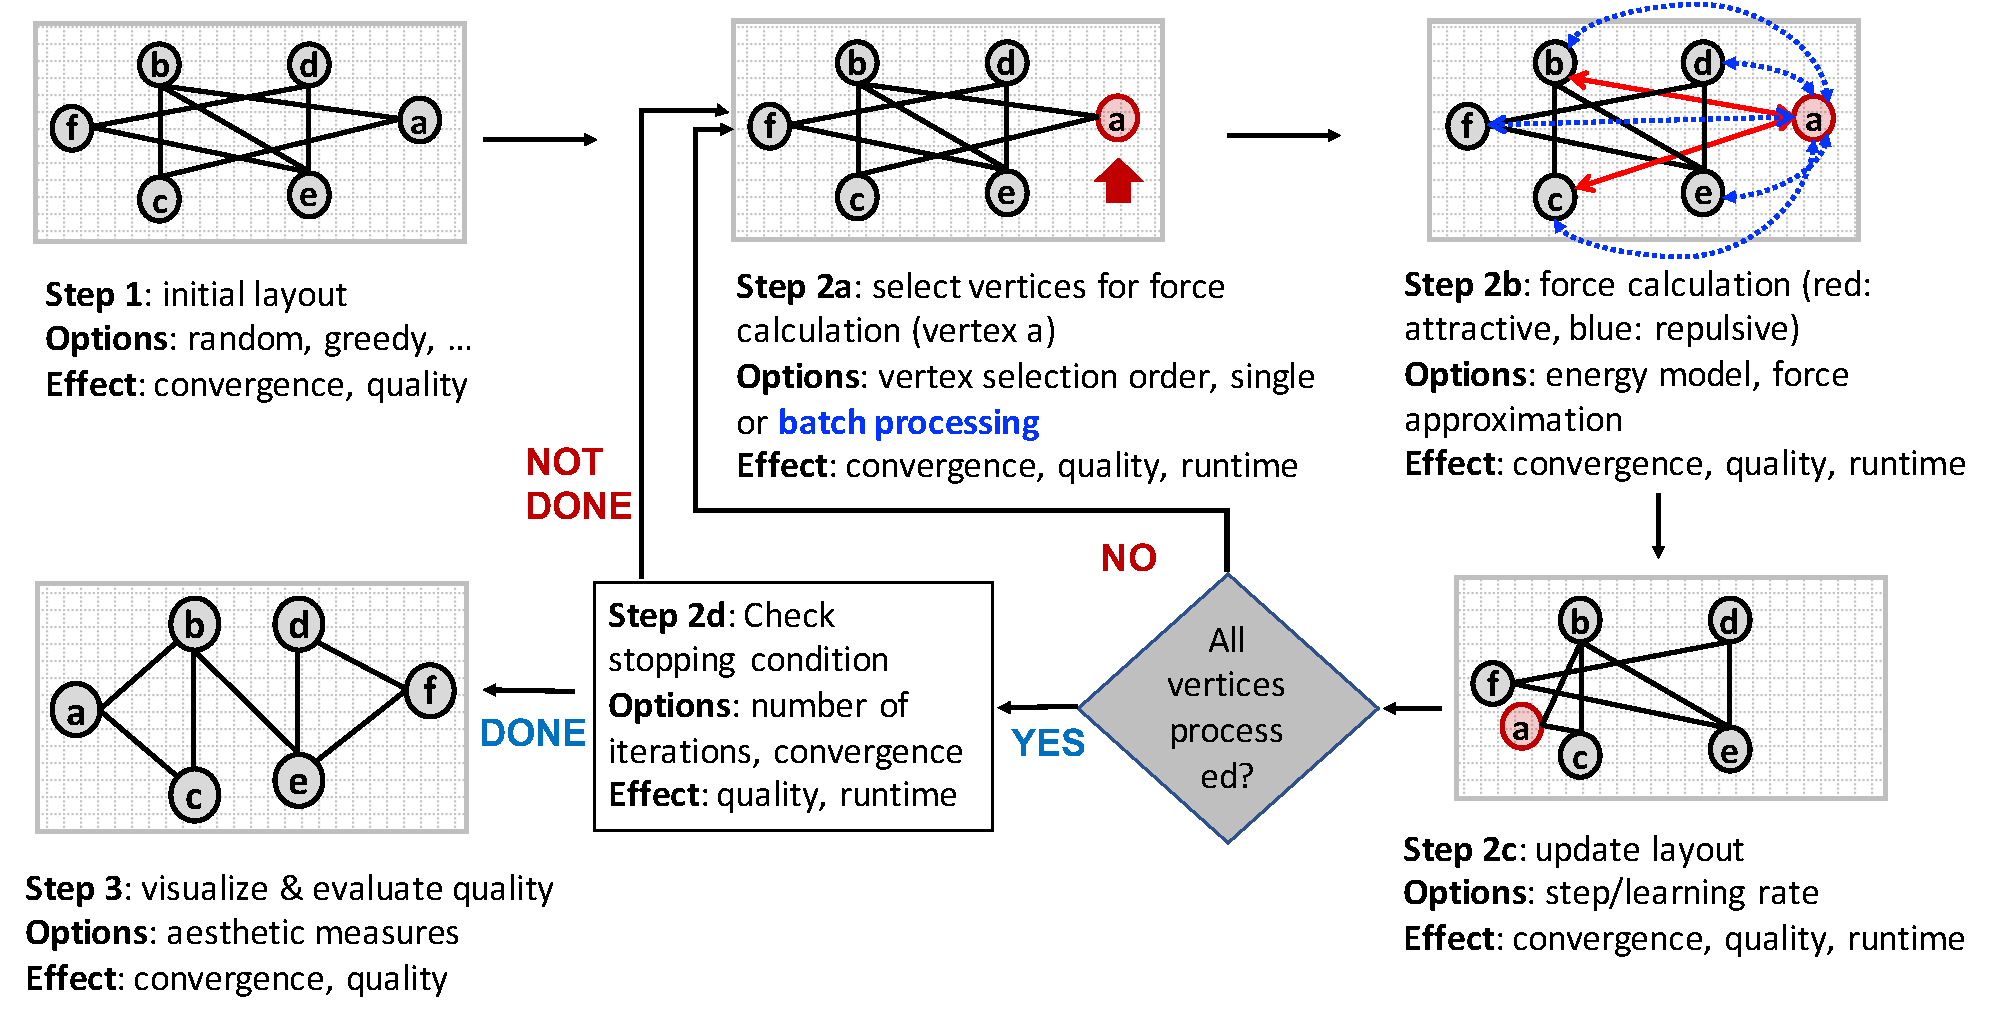
\includegraphics[width=0.9\linewidth]{figures/Force_directeed_flow}
    \vspace{-0.5cm}
    \caption{Steps involved in a typical force directed graph layout algorithm. An algorithm starts with an initial layout (usually a random layout) and iteratively updates the layout by calculating attractive and repulsive forces among vertices. When a stopping criterion is satisfied, the graph is visualized using the generated layout and the quality of the layout is evaluated. Each step has various algorithmic options that impact the convergence speed, the quality of the final layout, and the runtime of the algorithm. We highlighted ``batch processing" in Step 2a since it is a required option for efficient parallel algorithms discussed in this paper. We explored many options within our parallel algorithm.}
    \vspace{-0.4cm}
    \label{fig:batchlayoutsystem}
\end{figure*}




\subsection{A Standard Sequential Algorithm}
Algorithm~\ref{algo:sequential} describes a standard sequential force-directed graph layout algorithm. 
We closely followed the notation of an Adaptive Cooling Scheme by Y. Hu~\cite{hu2005efficient}. 
Algorithm~\ref{algo:sequential} starts with an initial layout and iteratively improves it by minimizing energy.
In each iteration, vertices are chosen in a predefined order (line 5), and attractive and repulsive forces are calculated for a selected vertex with respect to all other vertices in the graph.
Next, the relative position of the selected vertex is updated (line 12) and this updated position is used in processing the subsequent vertices. 
\emph{Step} used in line 12 is a hyper-parameter that influences the convergence of the algorithm.  
We will discuss possible values of this hyper-parameter in the experimental section.
A working example of this algorithm is shown in Fig. S1 of the supplementary file. 
%When attractive and repulsive forces are calculated for another vertex, updated position is considered for all previously updated vertices. 
Each iteration of Algorithm~\ref{algo:sequential} computes $O(m)$ attractive forces and $O(n^2)$ repulsive forces, giving us a sequential $O(n^2)$ algorithm.
Using the Barnes-Hut approximation~\cite{barnes1986hierarchical} of repulsive forces, Algorithm~\ref{algo:sequential} can easily be made into a sequential $O(n\log n)$ algorithm. 

\section{The \toolname{} Algorithm}

\subsection{Toward A Scalable Parallel Algorithm}
Despite its simplicity, it is hard to yield high performance from Algorithm~\ref{algo:sequential}.
A na\"ive parallelization of Algorithm~\ref{algo:sequential} can simply compute forces of a vertex in parallel by making line 7 of Algorithm~\ref{algo:sequential} a parallel loop. 
However, for vertex $i$, this na\"ive parallel algorithm offers $O(n+deg(i))$ parallel work for the exact algorithm and $O(\log n+deg(i))$ parallel work for the approximate algorithm.
To increase the parallel work, we followed the trend in training deep neural networks via SGD.
In traditional SGD, the gradient is calculated for each training example, which is then used to update model parameters.
Since SGD offers limited parallelism, most practical approaches use a batch of training examples (batch size varies from 256 to several thousands) to compute the gradient, an approach known as minibatch SGD.
We follow a similar approach by calculating forces for a batch of vertices and updating their coordinates in parallel. 
\toolname{} revolves around the batch processing of vertices and covers all other aspects of force-directed algorithms. 



\subsection{Overview of \toolname}
Figure~\ref{fig:batchlayoutsystem} shows the skeleton of a typical force-directed graph layout algorithm. 
After starting with an initial layout, an algorithm iteratively minimizes energy by computing attractive and repulsive forces.
Upon convergence, the final layout is drawn using a visualization tool. 
Figure~\ref{fig:batchlayoutsystem} shows that different steps of the algorithm have various choices upon which the quality and runtime of the algorithm depend. 
A comprehensive software such as ForceAtlas2 provides multiple options in each step. 
Like ForceAtlas2, \toolname{} also provides multiple options in each of these steps.
In particular, \toolname{} uses two initialization strategies, process vertices in different orders, considers four energy models, calculates exact and approximate repulsive forces, explores different learning rates and convergence conditions.
We evaluated the impact of different options on the convergence and quality of the algorithm.
We developed parallel algorithms for all options and evaluated their parallel performance. 


\subsection{Batch processing of vertices}
Since force calculations consume almost all computing time of our algorithm, we discuss parallel force calculation techniques first. 
As mentioned before, calculating forces for a single vertex does not provide enough work to keep many processors busy.
Hence, the \toolname{} algorithm selects a subset of vertices called a \emph{minibatch} and calculates forces for each vertex in the minibatch independently.
After all vertices in a minibatch finish force calculations, we update their coordinates in parallel.
Therefore, unlike Algorithm~\ref{algo:sequential}, the minibatch approach delays updating coordinates until all vertices in a minibatch finish their force calculations.
Fig. \ref{fig:BatchLayoutfig} illustrates this approach with a minibatch size of 2.

Batched force calculation has a benefit and a drawback. 
As we process more vertices simultaneously, we can keep more processors busy by providing ample parallel work. 
However, batch processing may slow down the convergence because the updated coordinates of a vertex cannot be utilized immediately. 
In our experiment, we observed that the benefit of concurrent work is significantly more than the disadvantage caused by slower convergence. 
Hence, batch processing makes a parallel algorithm significantly faster. 
%To make it clear, we describe the steps by Fig.  where graph has 6 vertices and size of minibatch is 2. 
%Similar to previous, we traverse graph sequentially i.e., we start from vertex $0$ and end in vertex $5$. Set of vertices in shaded region represents a minibatch (e.g. $\{0, 1\}$). At first, forces for vertex $0$ (green colored) are calculated and stored in a temporary variable. Similarly in next step, forces for vertex $1$ are calculated and stored in a temporary variable. Note that when forces for vertex $1$ are calculated, updated position of vertex $0$ is note considered as both $0$ and $1$ are in same minibatch of size 2. When computations of forces for all vertices in a minibatch are done, we update relative positions of each vertices as we did in next step represented by red colored vertices of $0$ and $1$. When we calculate forces for current subset of vertices (e.g., minibatch $\{2, 3\}$), we consider updated position of previous minibatches (e.g., minibatch $\{0, 1\}$) and this procedure goes on until all vertices are updated.

\begin{figure}[!htb]
    \centering
    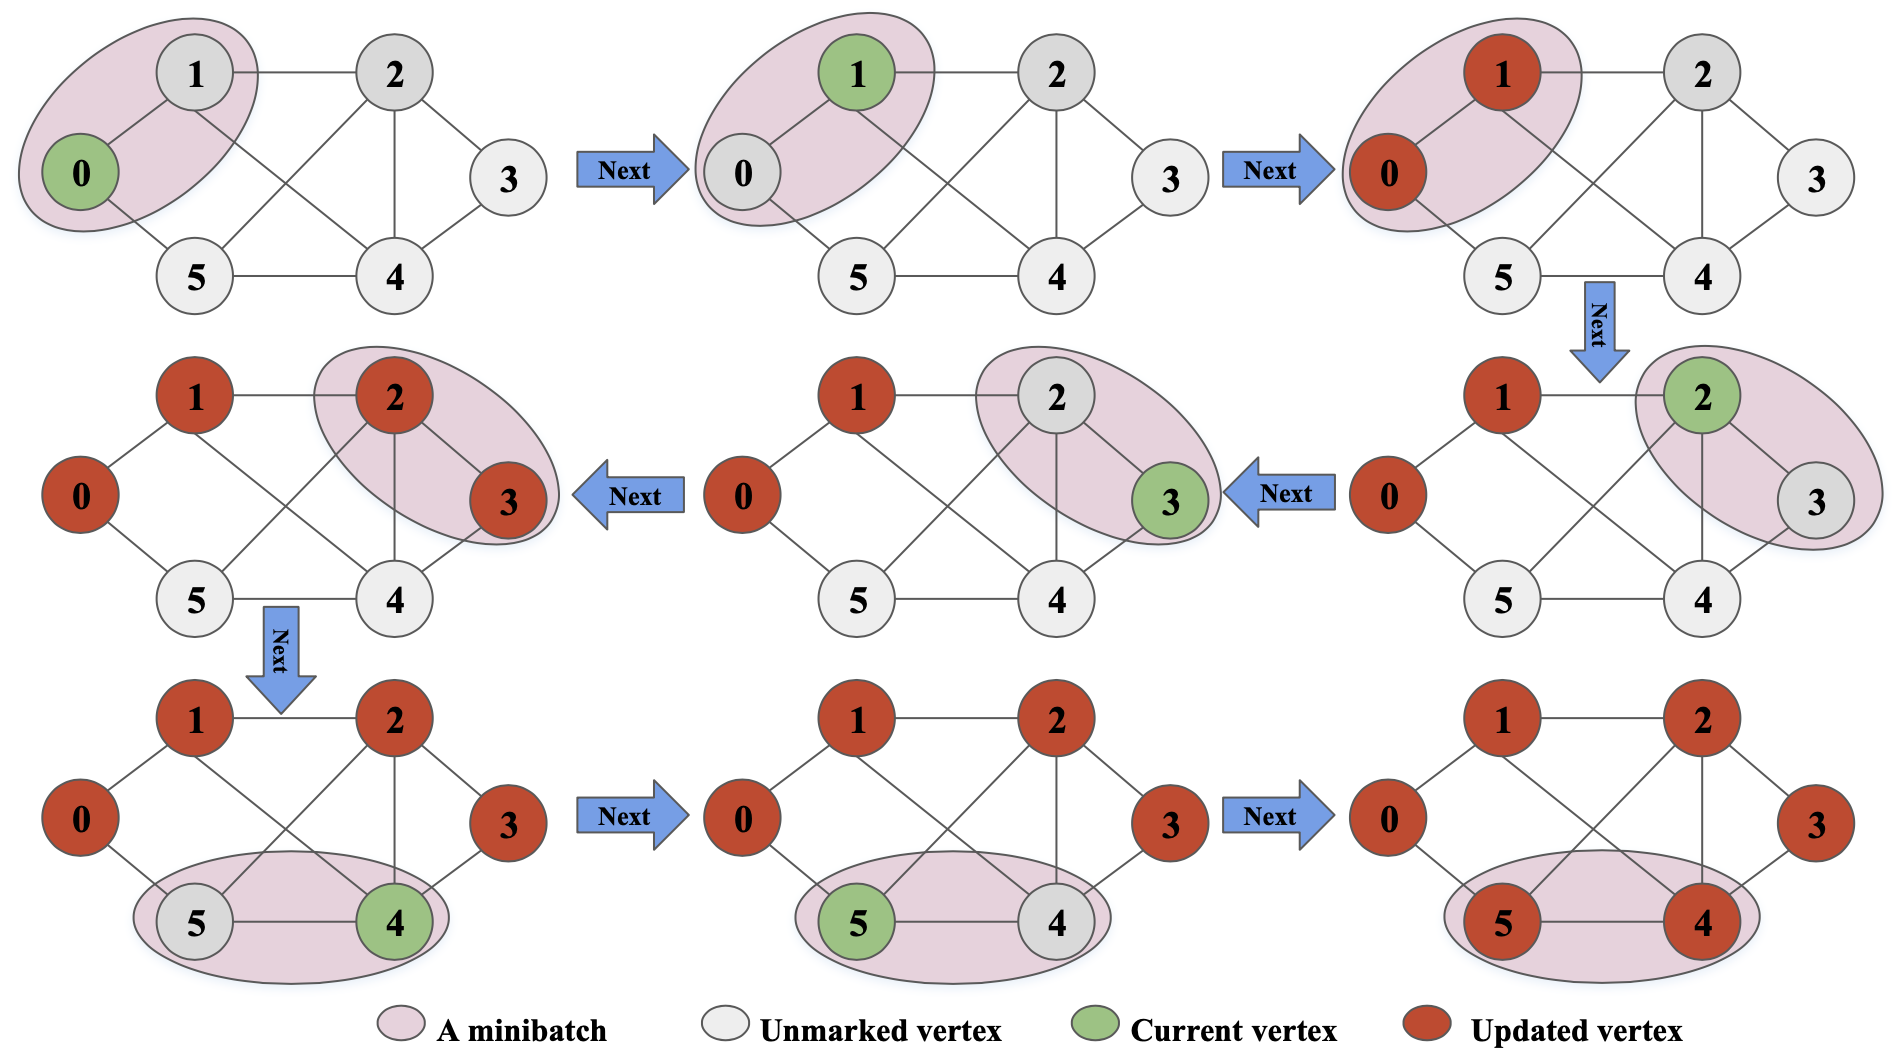
\includegraphics[width=\linewidth]{figures/smu.png}
    \caption{Force calculation with minibatch size 2. We start from vertex $0$ and consider two consecutive vertices in a minibatch shown in shaded regions. 
    This example finishes in three steps (each row in the figure), and each step processes a minibatch of two vertices.
    Green color denotes a vertex whose force is currently being computed, and red denotes a vertex whose coordinate is being updated. 
    In the first step (first row), vertex $0$ and vertex $1$ form a minibatch whose forces are first computed and then their coordinates are updated. 
    Similarly, in the second step (second row, from right to left), we calculate forces for vertex $2$ and $3$, and then update their coordinates. 
    Notice that in step 2, updated coordinates of the previous minibatch $\{0, 1\}$ are used.
    %vertex $0$ and $1$ are used in force calculation.
    %When we calculate forces for current subset of vertices (e.g., minibatch $\{2, 3\}$), we consider updated position of previous minibatches (e.g., minibatch $\{0, 1\}$) and this procedure goes on until all vertices are updated.
    }
    \vspace{-0.5cm}
    \label{fig:BatchLayoutfig}
\end{figure}

\begin{figure}
    \centering
    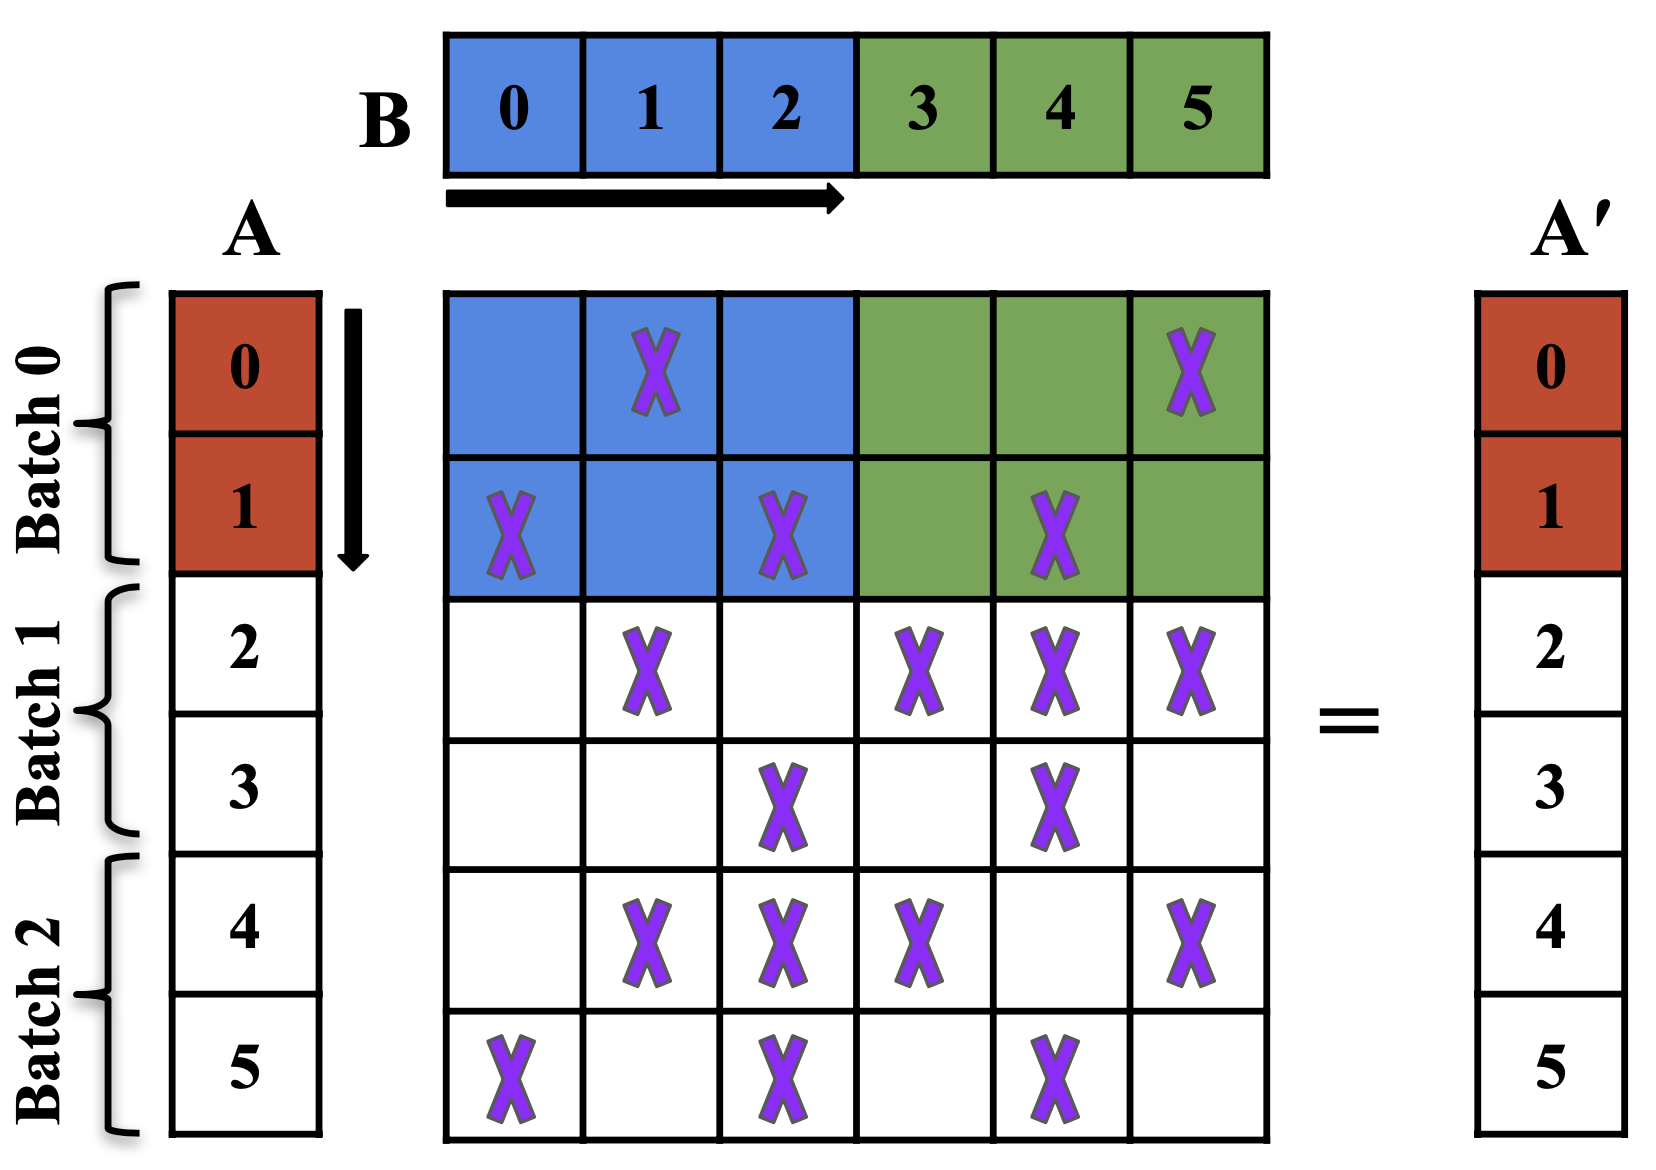
\includegraphics[width=0.7\linewidth]{figures/cacheblockingu.png}
    \vspace{-0.2cm}
    \caption{Computation of forces for the graph in Fig.~\ref{fig:BatchLayoutfig} using cache blocking technique. Here, the graph is stored as an adjacency matrix with `X' denoting edges between vertices. Vectors represents coordinates of vertices, and force calculations are viewed as a matrix-vector multiplication.
    %in a cell indicates a neighboring vertex that are commonly used in matrix-matrix or matrix-vector multiplication. An `X' in a cell indicates a neighboring vertex.
    }
    \vspace{-0.3cm}
    \label{fig:cacheblocking}
\end{figure}

\subsection{Improved Memory Accesses Via Cache Blocking}
While batch processing of vertices provides ample parallel work, processors can still remain idle if they have to wait for data to be fetched from memory.  
Memory stalling can happen if an algorithm does not utilize spatial and temporal locality in accessing data.
We addressed this issue by using cache blocking, a technique frequently used in linear algebra operations to utilize the cache hierarchy available in modern processors. 

%Notice that our problem is similar to sparse matrix-vector multiplication while calculating attractive force and dense matrix-vector multiplication while calculating repulsive force. 

%A straight forward implementation of the above approach can be efficient but may not utilize full advantage of modern cache performance. 

%Thus we further dig into the problem and deduce a highly scalable cache blocking version of \toolname{}. Cache blocking is a common technique in matrix-matrix or matrix-vector multiplication. 
%Notice that our problem is similar to sparse matrix-vector multiplication while calculating attractive force and dense matrix-vector multiplication while calculating repulsive force.

We noticed that force calculations can be viewed as a matrix-vector multiplication. 
Fig. \ref{fig:cacheblocking} shows a simple example where the adjacency matrix of the graph used in Fig.~\ref{fig:BatchLayoutfig} is considered.
The vector of current coordinates are shown twice in dense vectors A and B.
$A'$ holds the updated coordinates.
% A general intuition of cache blocking can be explained by a toy example as in Fig. \ref{fig:cacheblocking}. We assume that vectors $A$ and $B$ both hold the coordinates of a graph with 6 vertices, and $A'$ holds the updated coordinates as shown in Fig. \ref{fig:BatchLayoutfig}. 
In our minibatch model,  we compute the forces for all vertices in a minibatch with respect to all other vertices in the graph.
%where vectors $A$ and $B$ are literally same (i.e., $A = B$), though we show them separately for conceptual clearance. 
Suppose, in batch $0$, we compute forces for vertices $0$ and $1$ with respect to vertices $0 \ldots 2$ (blue). When forces are calculated for vertex $0$, coordinates of vertices $0 \ldots 2$ are brought in from the main memory and stored in a CPU cache.
%in L1 cache of the core, and 
The cumulative sum of force calculations are stored in a temporary vector, $A'$. 
When we compute forces for the next vertex $1$, all necessary coordinates are already available in cache (i.e., using data locality), which reduces the memory traffic. Batch $0$ gets a similar performance advantage when forces are computed with respect to vertices $3\ldots 5$ (green). 
\toolname{} with the cache-blocking scheme is presented in Algorithm \ref{algo:cbBatchLayout}. 
Here, {\myfont G.rowptr} and {\myfont G.colids} are two arrays which hold the row pointers and column IDs, respectively, of the graph in a CSR format. 
$BS$ is the size of minibatch and $Step$ length is initialized to $1.0$. 
In line $6$ of Algorithm \ref{algo:cbBatchLayout}, we iterate over a subset of vertices (minibatch) and in line $10$, we iterate over all vertices to calculate $f_a$ and $f_r$. 
In line $14$, when two vertices are connected by an edge we calculate $f_a$; otherwise, we calculate $f_r$ (line $18$). After calculating forces for a vertex, we store it in a temporary location (see line $19$). 
This temporary storage helps us to calculate forces in parallel. 
Next, we iterate over all vertices in a minibatch to update relative position (see line $22$).  
We provide a flexible rectangular cache blocking area which is bounded by variables $p$ and $q$. 
This increases the data locality in the L1 cache of each core, improving the performance of our algorithm. 
Loop counters $i$ and $j$ are increased by $p$ and $q$, respectively. 
Variable $k_x$ holds the starting index of neighbors for $p$ vertices (see line $8$). After the loop completes, in line $24$, we update step length. 
To keep Algorithm~\ref{algo:cbBatchLayout} simple, we assume that the number of vertices in a graph is multiple of $(b+1)*BS$.
In our implementation, we incorporated other cases.
%It can be easily seen that the number of vertices in a graph is not always a multiple of $(b+1)*BS$ and may introduce exceptions. For the sake of simplicity, we do not show such exception handling or conditional statements in Algorithm \ref{algo:cbBatchLayout}. 
The overall running time of this procedure is same as Algorithm \ref{euclid} i.e., $O(n^2)$. However, the main advantage of this technique is in parallel computation of forces. 
Note that Algorithm \ref{euclid} is a special case of Algorithm \ref{algo:cbBatchLayout} when the size of the minibatch is $1$.
 

\begin{algorithm}
\caption{Cache Blocking \toolname}
\hspace*{\algorithmicindent} \textbf{Input:} G(V, E)
\begin{algorithmic}[1]
\State $Step = 1.0$ \Comment{initial step length}
\State $Loop = 0$
\While {$ Loop < MaxIteration$}
\State $Energy = 0$
\For{$b \leftarrow$ 0 to $\frac{n}{BS}-1$}
    \ParFor{$i \leftarrow b * BS$ to $(b + 1) * BS-1$ \textbf{by} $p$}
        \For{$x \leftarrow 0$ to $p-1$}
            \State $k_{x} = G.rowptr[i+x]$
			\State $ct_{i+x} = 0$
        \EndFor
        \For{$j \leftarrow 0$ to $n-1$ \textbf{by} $q$}
            \For{$x \leftarrow 0$ to $p-1$}
            \State $f = 0$
                \For{$y \leftarrow 0$ to $q-1$}
                \If{$j + y == G.colids[k_x]$}
                    \State $f\;+= f_a(i,j)\times \frac{c_j - c_i}{\parallel c_i - c_j\parallel}$
                    \State $k_x\;+=1$
                \Else 
                    \State $f\; += f_r(i,j)\times \frac{c_j - c_i}{\parallel c_i - c_j\parallel}$
                \EndIf
                \EndFor
                \State $ct_{i+x} += f$ 
            \EndFor
        \EndFor
    \EndParFor
    \For{$i \leftarrow b * BS $ to $(b + 1) * BS - 1$}
        \State $c_i\; += Step \times \frac{ct_i}{\parallel ct_i\parallel}$
        \State $Energy\; += \parallel ct_i\parallel^2$
    \EndFor
\EndFor
\State $Step = Step \times 0.999$
\State $Loop += 1$
\EndWhile
\State \Return the final layout $c$
\end{algorithmic}
\label{algo:cbBatchLayout}
\end{algorithm}


\subsection{Repulsive Force Approximation}
Exact repulsive force computations need $O(n^2)$ time per iteration, which is too expensive for large graphs. 
Therefore, we have developed a parallel Barnes-Hut algorithm~\cite{barnes1986hierarchical} for approximating repulsive forces.
Barnes-Hut takes $O(n\log n)$ time per iteration. 
For 2D visualization, a quad-tree data structure is often used to approximate repulsive forces.
An example is shown in Fig.~\ref{fig:quadtree}. 
Given the coordinates of vertices in Fig.\ref{fig:quadtree}(a), a high-level block is divided into four equal blocks as shown in Fig. \ref{fig:quadtree}(b). 
In this example, we split up to $2$ levels, creating $4^2 = 16$ small blocks in the 2D plane. 
Empty blocks are merged with their adjacent nonempty blocks. 
We show how the algorithm approximates the repulsive force $f_r$ for the green vertex.
First, a centroid (shown in red) is calculated for each block by averaging the coordinates of all vertices in the block. 
Next, an approximate repulsive force is computed with respect to the centroids, as shown by the dashed gray lines. 
%Additionally,  solid lines show attractive force calculations with respect to adjacent vertices. 

%For all other non-neighboring vertices (a block containing one vertex), $f_r$ is calculated as it is. Note that for the block located in right bottom corner, we can calculate $f_r$ with respect to only one centroid instead of four vertices individually which reduces running time in $f_r$ calculations. In this procedure, quad-tree data structure can help to store information of 2D space partitioning in efficient way.


%calculations to minimize the running time \cite{barnes1986hierarchical} which asymptotically takes $O(n\log n)$ time, where $n$ is the number of objects (vertices in case of force-directed graph layout). 
%Quad-tree (Oct-tree) structure is maintained for such approximation in 2D (3D). Most of the real-world graphs takes significant amount of time for repulsive force ($f_r$) calculations. Thus approximation of $f_r$ is a major advantage for running time though it sacrifices quality of the layout a little.

%We have shown an example for repulsive force approximation in Fig. \ref{fig:quadtree}. In each split, a block is divided into four equal blocks as shown in Fig. \ref{fig:quadtree}(b). In this example, we split up to $2$ levels which creates $4^2 = 16$ small blocks in the 2D plane. Note that some adjacent blocks have been merged due to absence of any vertex. When we calculate $f_a$ and $f_r$ for green colored vertex located in upper left corner, we can approximate $f_r$ as following: a centroid is calculated for each block by averaging the coordinates of all vertices in the block. In Fig. \ref{fig:quadtree}(c), red colored points are centroids of corresponding blocks where there are more than one vertex in a block. Gray dotted line shows $f_r$ with respect to centroids. Blue solid line shows $f_a$ with respect to neighbors. For all other non-neighboring vertices (a block containing one vertex), $f_r$ is calculated as it is. Note that for the block located in right bottom corner, we can calculate $f_r$ with respect to only one centroid instead of four vertices individually which reduces running time in $f_r$ calculations. In this procedure, quad-tree data structure can help to store information of 2D space partitioning in efficient way.

\begin{figure}[!t]
    \centering
    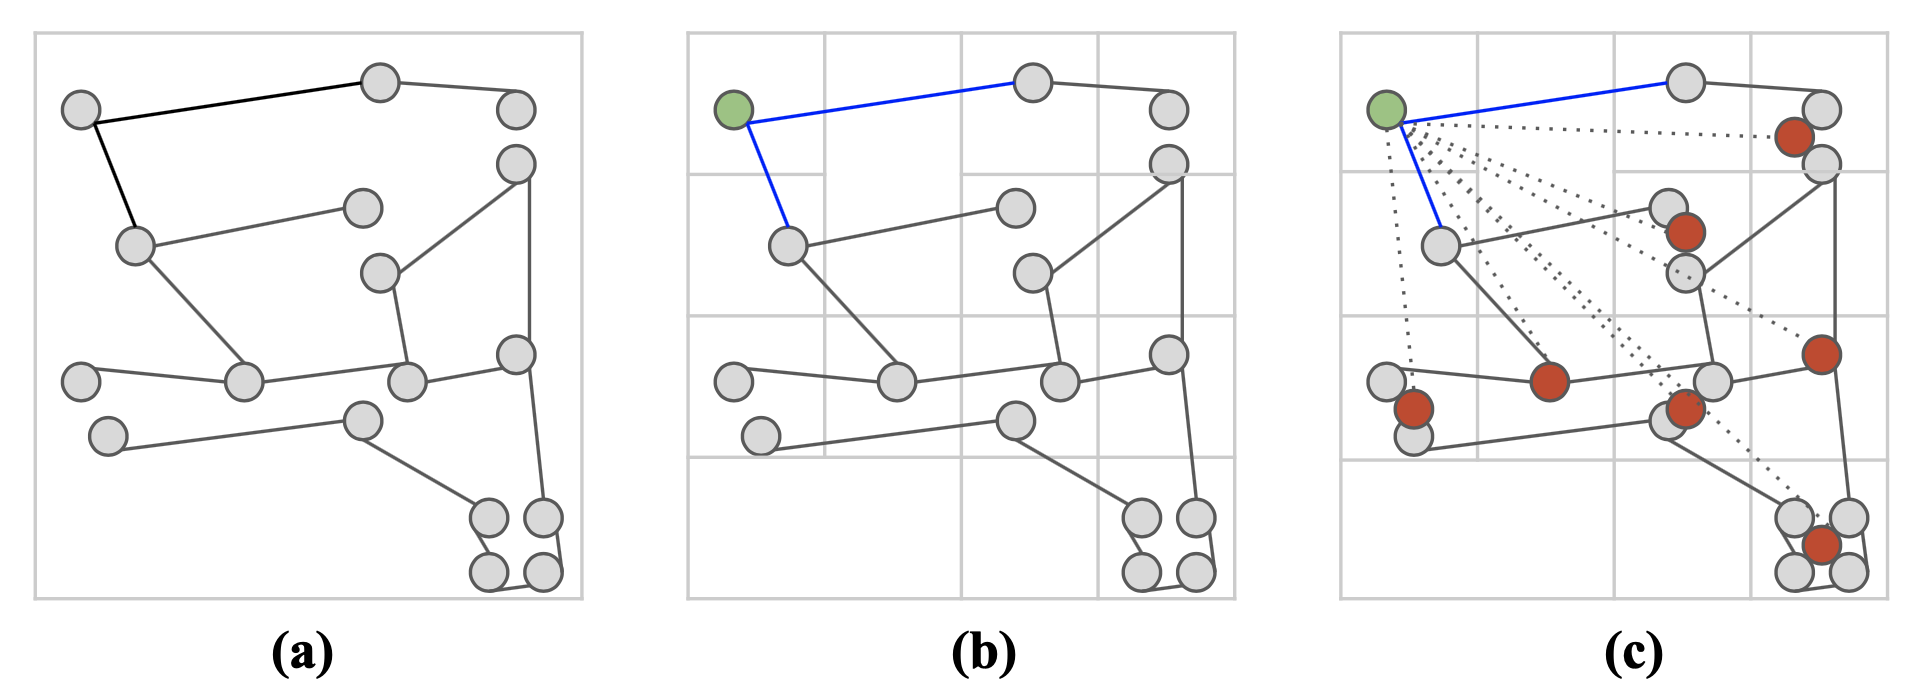
\includegraphics[width=\linewidth]{figures/quadtreeexampleu.png}
    \vspace{-0.7cm}
    \caption{(a) An example graph. (b) Calculating forces of the green vertex using a quad-tree. (c) Blue solid lines show attractive forces, and dashed gray lines denote approximate repulsive forces with respect to centroids (red).}
    \vspace{-0.3cm}
    \label{fig:quadtree}
\end{figure}

\begin{figure}[!t]
    \centering
    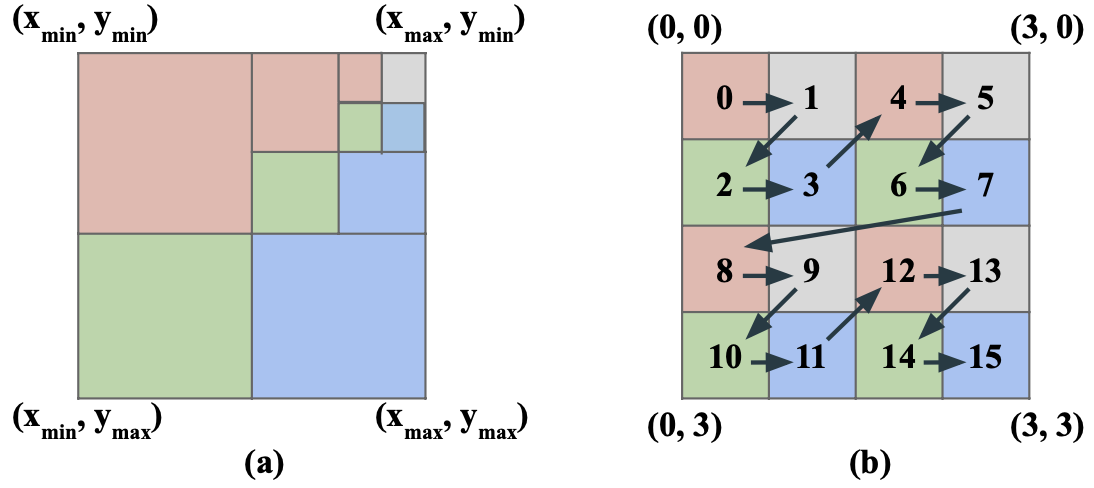
\includegraphics[width=\linewidth]{figures/hashedquadtree.png}
    \vspace{-0.6cm}
    \caption{(a) A quad-tree structure. (b) Morton order of traversal for 16 vertices in 16 different blocks.}
    \vspace{-0.6cm}
    \label{fig:hashedquadtree}
\end{figure}

Among several choices of quad-tree implementation~\cite{zhang2014design}, we adopted an approach based on Warren and Salmon \cite{warren1993parallel}. 
Fig. \ref{fig:hashedquadtree}(a) shows that we define a drawing plane by bounding coordinates $(x_{max}, y_{max})$ and $(x_{min}, y_{min})$. 
This bounding plane is the root of the quad-tree.
Next, we split the bounding plane (root) into four equal blocks, each of which represents a child node (shown by a unique color) of the root. 
%We implement quad-tree in similar way as done by Warren and Salmon \cite{warren1993parallel}. 
We sort the positions of all vertices based on Morton code (also called Z-order curve)~\cite{morton1966computer} and obtain an ordered list of vertices.
This ordering basically represents the Depth First Search (DFS) traversal of a quad-tree. 
Fig. \ref{fig:hashedquadtree}(b) shows a possible Morton ordering of a graph with 16 vertices. % where each block of width $D$ contains one vertex. 
From the Morton ordering, we recursively build the tree, where leaf nodes represent vertices in the graph, and an internal node stores its centroid which is computed from its children.

Basically, nearer non-adjacent vertices contribute more than far vertices to $f_r$. For this reason, a threshold ($\theta$) is set to determine relative distance between two vertices while calculating $f_r$. 
A Multipole Acceptance Criteria (MAC), $\theta > \frac{D}{\parallel c_i - c_j \parallel}$ is evaluated while traversing the tree for $f_r$ calculations. If MAC is {\myfont\textbf{true}} then two vertices are located at far enough distance such that the current centroid can approximate that repulsive force. In this way, $f_r$ calculation can be approximated in $O(\log n)$ time which has been discussed elaborately \commentKhaled{in \cite{hu2005efficient,hachul2004drawing}}, thus, the overall running time becomes $O(n\log n)$ per iteration. We use the term \toolnameBH{} to describe this version and provide full pseudo-code in supplementary file, Algorithm S3.


%There are also hashed based implementation for distributed memory \cite{warren1993parallel,winkel2012massively} which have been found effective in Message Passing Interface (MPI). 
%A general intuition of quad-tree is space partitioning. For example, we bound the drawing space exclusively by coordinates $(x_{max}, y_{max})$ and $(x_{min}, y_{min})$. Then we equally split the bounding space (root) into four equal blocks as shown in Fig. \ref{fig:hashedquadtree}(a) each of which represents a child node (unique color) of the root. We implement quad-tree in similar way as done by Warren and Salmon \cite{warren1993parallel}. At first, we sort the positions of all vertices based on Morton code \cite{morton1966computer} and get an ordered list of vertices which basically represents the DFS traversal of quad-tree. In Fig. \ref{fig:hashedquadtree}(b), we show a possible morton ordering of a graph with 16 vertices where each block of width $D$ contains one vertex. After that, we recursively build the tree. The leaf nodes of the tree represents vertices in the graph and each internal node of the tree calculates centroid based on its children. Basically, nearer non-adjacent vertices contribute more than far vertices to $f_r$. For this reason, a threshold ($\theta$) is set to determine relative distance between two vertices while calculating $f_r$. A Multipole Acceptance Criteria (MAC), $\theta > \frac{D}{\parallel c_i - c_j \parallel}$ is evaluated while traversing the tree for $f_r$ calculations. If MAC is {\myfont\textbf{true}} then two vertices are located at enough distant such that current centroid can approximate that repulsive force. In this way, $f_r$ calculation can be approximated in $O(\log n)$ time which has been discussed elaborately by Yifan Hu \cite{hu2005efficient} and thus the overall running time becomes $O(n\log n)$ per iteration. We term this version as \toolnameBH{}.

%In this paper, we calculate $f_r$ based on the sorted order of vertices which become more cache friendly.



\subsection{Initialization}
The initial layout plays an important role in the convergence and visualization quality of the final layout.
\commentKhaled{Many existing algorithms start with random layouts where vertex positions are assigned randomly~\cite{hu2005efficient}.}
%Generally, an algorithm starts with a random layout where vertex positions are assigned randomly~\cite{hu2005efficient}. 
%Some methods also assign initial coordinates to zero \cite{martin2011openord}.
%This part is independent of optimizing combined force that we discussed in Algorithm \ref{algo:cbBatchLayout}; however, it may play important role in faster convergence. 
In addition to random initial layouts, we developed a novel greedy initialization technique as shown in Algorithm \ref{algo:greedy}. 
We maintain a \emph{stack} $S$ to keep track of visited vertices.
The algorithm starts with a randomly selected vertex $V_0$, and $(0,0)$ is used as its coordinate. 
In every iteration, the algorithm extracts a vertex $U$ from the stack and places $U$'s neighbors on a unit circle centered at $U$ (line $10-14$ in Algorithm \ref{algo:greedy}).
Additionally, the distance between every pair of $U$'s neighbors is also equal.
In line $12$, $PI$ is a constant whose value is $3.1416$. 
In section \ref{subsec:uel}, we will discuss that uniform edge length is a good aesthetic metric for assessing the quality of a layout. 
Hence, we consider this unit-radius approach  to be a better initializer.
Our experimental results does show that the greedy initialization indeed converge faster than the random initialization. 
The greedy approach is similar to a DFS with $O(n+m)$ complexity.



%We then iterate over neighbors of that vertex (line $10$ in Algorithm \ref{algo:greedy}) to initialize in a circular way around it with unit radius and equal distant. 


\begin{algorithm}[!t]
\caption{Greedy Initialization}
\hspace*{\algorithmicindent} \textbf{Input:} G(V, E)
\begin{algorithmic}[1]
\State $S = \emptyset $ \Comment{initial empty stack}
\State $visited = [False, \ldots, False]$
\State $V_0 = (0, 0)$ \Comment{$V_{0x} = 0, V_{0y} = 0$}
\State $S.push(V_0)$
\State $visited_0 = True$
\While {$S$ is not empty}
\State $U = S.pop()$
\State $d = \frac{360}{deg(U)}$
\State $D = 0$
\For{$u$ neighbors of $U$}
    \If{$visited_u$ is $False$}
        \State $V_u = (U_x + cos(\frac{PI*D}{180.0}), U_y+sin(\frac{PI*D}{180.0}))$
        \State $visited_u = True$
        \State $S.push(V_u)$
        \State $D = D + d$
    \EndIf
\EndFor
\EndWhile
\State \Return $V$
\end{algorithmic}
\label{algo:greedy}
\vspace{-0.4cm}
\end{algorithm}


%\subsubsection{Shared Memory Parallelism}
%We have implemented all of our Algorithms in OpenMP \cite{dagum1998openmp}. It provides several compiler directives to easily implement in parallel environment using multi-core architecture. It also provides three loop scheduling schemes, namely, {\myfont static}, {\myfont dynamic} and {\myfont guided} which have advantages based on solution approach. As there are $p$ threads to run in parallel, the asymptotic running time of cache blocking version of \toolname{} is $O(\frac{n^2}{p})$ and for quad-tree approximation, it is $O(\frac{n\log n}{p})$. 

%\subsubsection{Setting LinLog and Edge Weight}We want to make more options available in \toolname{}. As a step towards it, we have employed popular linlog mode \cite{noack2003energy} and edge weight mode so that those options can also take advantage of high performance cache coherent implementation. 

%\subsubsection{Greedy Force Approximation}
%In this mode of repulsive force calculations, we only consider 150-200 vertices that are in $n$-hops distant. We set this mode in such a way that it calculates $f_r$ in first $80\%$ iterations using greedy approach and last $20\%$ iterations using general approach as described in Algorithm \ref{algo:cbBatchLayout}. The purpose of last $20\%$ iterations is that it compensates force approximation so that the quality of final layout is adorable.  We have also made another option available in our tool where first 80\% time is used in \toolnameBH{} and last 20\% time is used in \toolname{} to generate layout. This option generates good layout in promising running time.

\subsection{Performance Metrics}
\label{sec:aesthetic_measure}
There are several aesthetic metrics in the literature to assess the quality of a layout generation algorithm \cite{purchase2002metrics,kwon2017would,de2019multi}. Though there does not exist a single metric that can uniquely determine the effectiveness of a layout, it gives a quantitative value that tells us how layout algorithms perform. For the sake of completeness, we have used the following aesthetic metrics along with running time analysis.

%{\bf Edge Crossing (EC): }
%Edge crossing has been found to be an important aesthetic measure in many studies \cite{huang2007effects}; it basically computes the number of edge crossing points in a layout. This implies that a lower number of edge crossing points represents a better layout. Some studies normalize this value between 0 to 1 where $1$ indicates better layout \cite{purchase2002metrics}. In this paper, we only report the edge crossing number as in some cases, the normalized value does not reflect the actual measurement.

{\bf Stress (ST): }
Stress computes the difference between geometric distance and graph theoretic distance for any pair of vertices in a graph~\cite{brandes2008experimental,de2019multi}. Since different algorithms may require different drawing space based on which stress may change, the drawing space is scaled before computing the stress for all algorithms. Thus, the reported value is the minimum value achievable after scaling the layout. A lower ST value indicates a better layout, and it is computed using $\sum_{i,j\in V} w_{ij}(\parallel c_i - c_j\parallel - d_{ij})^2$ where, $c_i$ and $c_j$ are coordinates of vertices $i$ and $j$, respectively. The value of $d_{ij}$ represents a graph theoretic distance between vertices $i$ and $j$, and $w_{ij} = \frac{1}{d_{ij}^2}$.


%\subsubsection{Minimum Angle (MA)}
%The minimum angle is another aesthetic metric which computes the average absolute deviation of adjacent incident edge angles from the ideal minimum angle \cite{purchase2002metrics}. This metric can be computed using following equation:

%\begin{equation*}
%    MA = 1 - \frac{1}{|V|}\sum_{v\in V}|\frac{\theta(v) - \theta_{min}(v)}{\theta(v)}|
%\end{equation*}
%where, $\theta(v) = \frac{360}{deg(v)}$ and $\theta_{min}(v)$ is the minimum angle between the incident edges on vertex $v$. Higher value of $MA$ represents better layout.

{\bf Edge Uniformity (EU):}
\label{subsec:uel}
Sometimes the uniformity of edge lengths represents better readability of a layout \cite{huang2007effects}. We define EU in a similar way as defined in \cite{hachul2007large,de2019multi}. It finds the normalized standard deviation of edge length which can be computed using $\sqrt{\frac{\sum_{e\in E}(l_e - l_{\mu})^2}{|E|.l_{\mu}^2}}$ where, $l_{\mu}$ is the average length of all edges and $|E|$ represents the number of edges in the graph. Lower value of EU represents better quality of the layout.

{\bf Neighborhood Preservation (NP): }
This measure computes the number of neighbors that are close to a vertex in a graph as well as in the driven layout. It has been used to compare graph layouts in many tools like tsNET \cite{kruiger2017graph} and Maxent \cite{gansner2012maxent}. This is a normalized similarity measure where $0$ means that the adjacency of vertices are not preserved in the layout whereas $1$ means that all vertices preserve their respected neighbors.

\section{Results}

\subsection{Experimental Setup}
We implemented \toolname{} in C++ with multithreading support from OpenMP.
%which requires at minimum GCC version 4.9 and OpenMP version 4.5. 
We ran all experiments in a server consisting of Intel Xeon Platinum 8160 processors (2.10GHz) arranged in two NUMA sockets. 
The system has 256GB memory, 48 cores (24 cores/socket), and 32MB L3 cache/socket. 
%2.10GHz, 32KB L1 cache, 1MB L2 cache, 32MB L3 cache, 48 cores and 2 NUMA nodes with 256GB memory. 
For comparison, we used ForceAtlas2 implemented in Gephi and OpenOrd from its  GitHub\footnote{https://github.com/SciTechStrategies/OpenOrd} repository.
We also experimented with Gephi's OpenOrd implementation (denoted by OpenOrdG), but found that the GitHub implementation produced better visualizations. 
We use Gephi's toolkit v0.9.2 \cite{bastian2009gephi} to run multi-threaded ForceAtlas2 and OpenOrdG. 
The Barnes-Hut variant of ForceAtlas2 is termed as ForceAtlas2BH. 
For \toolnameBH{}, we use the same threshold value ($1.2$) for MAC as in ForceAtlas2BH. 
Unless otherwise specified, we use the default settings for all of these tools.
For OpenOrd, we set the edge-cutting parameter to $0$, and we set the default time distribution in different stages of simulated annealing. 
While the \toolname{} software includes four variants of $(a,r)$-energy model considered in the ForceAtlas2 paper, we only show results from \toolname{} using $(2,-1)$-energy model (equivalent to the Fruchterman and Reigngold algorithm).
We selected this model because it usually generates better visualizations~\cite{jacomy2014forceatlas2}.



%We run all experiments in a server machine which is configured as following: Intel\textsuperscript{\textregistered} Xeon\textsuperscript{\textregistered} Platinum 8160 CPU\textcopyright2.10GHz, 32KB L1 cache, 1MB L2 cache, 32MB L3 cache, 48 cores and 2 NUMA nodes with 256GB memory. We compare our results with other spring-electrical based tools like OpenOrd, and Gephi's ForceAtlas2 and OpenOrd which are some of the current state-of-the art tools. We term OpenOrd to represent the original tool from authors' GitHub\footnote{https://github.com/SciTechStrategies/OpenOrd} repository and OpenOrdG to represent Gephi's OpenOrd. Notably, we observe some differences between OpenOrd and OpenOrdG in our experiments. We also run tsNET \cite{kruiger2017graph} to conduct some experiments though it is very slow and not effective for big graph visualization. We run tsNET tool using only one thread as it has no multi-threaded version and set perplexity and learning rate as 800 and 6000, respectively. We observe that it can generate good layout for small graphs but failed to generate any layout for medium or bigger graphs in our experiments. We use Gephi's toolkit v0.9.2 \cite{bastian2009gephi} to run multi-threaded ForceAtlas2 and OpenOrdG. The Barnes-Hut version of ForceAtlas2 is termed as ForceAtlas2BH. For both version of OpenOrd, we set edge cutting parameter as $0$ and default time distribution in different stages of simulated annealing. For \toolnameBH{}, we use same threshold value ($1.2$) for MAC as in ForceAtlas2BH. Unless otherwise noted, we use default settings for all of these tools.

\begin{table}[]
\caption{Graphs used in our experiments. $|V|$ and $|E|$ represent number of vertices and edges, respectively. d means average degree.}
\vspace{-5pt}
\centering
\begin{tabular}{|p{1.35cm}|p{1.15cm}|p{1.34cm}|c|p{1.7cm}|}
\hline
\textbf{Graph} & \textbf{$|V|$} & \textbf{$|E|$} & \textbf{d} & \textbf{Type}\\ \hline
Powergrid             &      4,941	               &   13,188                &        	2.66              & Small World \\ \hline
add32            &     	4,960                &   	19,848                  & 	3.00       &   Scale Free  \\ \hline
ba\_network	           &      6,000	                &    5,999            &    	1.99                     & Scale Free \\ \hline
3elt\_dual	          & 9,000          & 	26,556	         &     2.95                  & Mesh \\ \hline
PGP           &         	10,680              &  	48,632	                &    4.55                 & Scale Free \\ \hline
pkustk02           &         	10,800             &      	399,600	             &        76              & Feiyue twin tower\\ \hline
fe\_4elt2	           &      11,143               &   	65,636	                & 5.89        &   Mesh  \\ \hline
bodyy6	           &        19,366              &    	134,208	                &        5.93             & NASA Mat.\\ \hline
%tube2   &	21,498  &	897,056 &	40.72 & Structural Problem \\ \hline
pkustk01	            &       22,044               &         	979,380         &      	45.42               & Beijing bot. exhib. h. \\ \hline

OPF\_6000   &	29,902	&   274,697	    &   8.66    &  Ins. of Pow. Sys. G. U. \\ \hline
finance256	&   37,376	    &   298,496	    &   6.98    &   Lin. Prog. \\ \hline
%gridgena	           & 48,962	            & 512,084          &    9.4                &  Optimization Problem\\ \hline
finan512    &	74,752	    &   261,120	    &   6.98    &   Eco. Prob. \\ \hline
lxOSM	&   114,599 &	239,332 & 2.08 & Op. St. Map \\ \hline
comYoutube	&   1,134,890 &	5,975,248   & 5.26  & Social Net. \\ \hline
%af\_shell10	&   1,508,065 &	52,259,885   & 33.65  & Structural Problem \\ \hline
Flan\_1565	&   1,564,794	&   114,165,372   & 71.95  & Struc. Prob. \\ \hline
\end{tabular}
\label{tab:datasets}
\vspace{-0.5cm}
\end{table}

\subsection{Datasets}
\label{lab:datasets}
Table \ref{tab:datasets} shows a diverse collection of test graphs including small world networks, scale free networks, mesh, structural problem, optimization problem, linear programming, economic problem, social networks, and road networks. 
These graphs were collected from the SuiteSparse matrix collection (https://sparse.tamu.edu).
Specifically, we use Luxembourg OSM (lxOSM) and Flan\_1565 datasets to test the ability of algorithms to visualize large-scale graphs. 
For scalability experiments, we also generated benchmark networks by Lancichinetti et al.~\cite{lancichinetti2008benchmark}. 
For this tool, we set mixing parameter, avg. degree, community minsize, community maxsize to 0.034, 80, 128 and 300, respectively, and vary maximum degree from 100 to 300. 
We generated a total of 5 random graphs, each of which has $2^v$ vertices, where $v \in \{16, 17, 18, 19, 20\}$. 

\subsection{Algorithmic Options and Their Impacts}
\subsubsection{Initialization}
At first, we compare the differences between greedy initialization using Algorithm \ref{algo:greedy} and random initialization using the C++ function {\myfont rand}.
Both initialization techniques generate random coordinates within a given range {\myfont [-MAXMIN, MAXMIN]}.
We feed initial coordinates to \toolname{}, and Fig. \ref{fig:selfcheckout}(a) shows the layout energy for  the \emph{3elt\_dual} graph after various iterations. 
We observe that in the $i^{th}$ iteration, the greedy-initialized layout has lower energy than  the randomly-initialized layout.
This result is consistent across other graphs as well.
Fig. \ref{fig:selfcheckout}(a) reveals that greedy initialization accelerates the convergence of \toolname{}.
Hence,  we use the greedy initialization in subsequent experiments in the paper (both initializations are available in our software).




%For this experiment, we have used \emph{3elt\_dual} graph and made sure that all vertices are initialized within same boundary value i.e., we generate random coordinates within range {\myfont [-MAXMIN, MAXMIN]} then for greedy procedure we scale all coordinates so that they lie within range {\myfont [-MAXMIN, MAXMIN]}. Then we feed these initial coordinates to \toolname{} and results are shown in Fig. \ref{fig:selfcheckout}(a) for different number of iterations. We observe that the \emph{Energy} of greedy initialization technique is always smaller than random technique and found this result consistent across several graphs. So, we select this greedy initialization technique for all of our next experimental results; however, we have kept both initialization techniques available in our tool.


%We have compared acceleration of convergence between greedy initialization and random initialization technique. For greedy technique, we have used Algorithm \ref{algo:greedy} and 
%for random technique we have used built-in {\myfont rand} function of C++. For this experiment, we have used \emph{3elt\_dual} graph and made sure that all vertices are initialized within same boundary value i.e., we generate random coordinates within range {\myfont [-MAXMIN, MAXMIN]} then for greedy procedure we scale all coordinates so that they lie within range {\myfont [-MAXMIN, MAXMIN]}. Then we feed these initial coordinates to \toolname{} and results are shown in Fig. \ref{fig:selfcheckout}(a) for different number of iterations. We observe that the \emph{Energy} of greedy initialization technique is always smaller than random technique and found this result consistent across several graphs. So, we select this greedy initialization technique for all of our next experimental results; however, we have kept both initialization techniques available in our tool.

\subsubsection{Minibatch size}
We now select a minibatch size that provides enough parallelism without affecting the convergence rate significantly.
Fig. \ref{fig:selfcheckout}(b) shows layout energies for different minibatches for the \emph{pkustk02} graph.
Here, BL256 denotes \toolname{} with minibatch size of 256.
For this graph, we observe that small minibatches converge faster (in terms of iterations) than large minibatches. 
For example, BL1 and BL256 achieve the same energy at 1000 and 1100 iterations, respectively (marked by brown squares in Fig. \ref{fig:selfcheckout}(b)). 
Consequently, BL256 needs to run 100 more iterations to reach the same energy achieved by BL1.
However, the cost of extra iterations is offset by faster parallel runtime of BL256.
Fig.~\ref{fig:selfcheckout}(c) shows the runtime for different minibatches when we run \toolname{} with 48 threads for the same graph \emph{pkustk02}.
To achieve the energy level marked by brown squares, BL1 takes around 433.6 seconds, whereas BL256 takes only 9.7 seconds.
That is, BL256 is $\sim 40\times$ faster than BL1 despite the former taking 100 more iterations than the latter to reach the same layout energy.
For this reason, minibatches play a central role in attaining high performance by our parallel algorithm.
However, using larger minibatches beyond 256 does not improve the performance further.
For example, BL256 and BL2048 behave almost similarly as can be seen in Figs. \ref{fig:selfcheckout}(b) and \ref{fig:selfcheckout}(c).
We also observe similar minibatch profiles for other graphs. Hence, we set 256 as the default minibatch size for the rest of our experiments (a user can change the minibatch size in our software). 


%\subsubsection{Batch size}
%We conduct another experiment to choose effective batch size that will be faster towards convergence with reasonable running time. We empirically found that this result is consistent for graphs with higher average degree. We show the results of \emph{pkustk02} graph in Figs. \ref{fig:selfcheckout}(b) and \ref{fig:selfcheckout}(c) for several batches and iterations using 48 threads. BL$n$ represents a batch of size $n$. For the example graph, we see that small batches converge faster across iterations than large batches which is expected (Fig. \ref{fig:selfcheckout}(b)). For example, BL1 and BL256 achieve same level of \emph{Energy} around 1000 and 1100 iterations, respectively (marked as brown square box in Fig. \ref{fig:selfcheckout}(b)). As described earlier, our intuition is that BL256 will take less time to run for 1100 iterations than what BL1 takes to run for 1000 iterations. In Fig. \ref{fig:selfcheckout}(c), we show corresponding running time where we see that BL256 takes only around 9.7 seconds whereas BL1 takes around 433.6 seconds. B256 is faster because it offers more parallelism than BL1. We also notice here that BL256 optimizes more faster than BL512 and their run-times are approximately same. So, a trade-off between convergence and run-time is important to select a batch size. We have kept this as an option in our tool; however, after doing a rigorous set of experiments on several graphs we use a batch of 256 vertices for all of our next experimental results.


\subsubsection{Batch Randomization}
We conduct experiments for the randomization of batches which is a common practice in machine learning. We reported standard deviation as well as energy curves for different runs using \emph{3elt\_dual} graph (Figure S3 in supplementary file). From our experiments, we observed that randomized batch selection achieves better energy curve than fixed sequential batch selection but results are not deterministic i.e., for each run, output is different (similar but not same) even though all hyper-parameters are same. We can see a greater difference for a smaller number of iteration. Randomization also introduces overhead in total running time for reshuffling and it can not take advantage of optimal cache usage. Moreover, randomized batch selection does not make any significant improvement in layout. So, we keep sequential batch selection as our default option in \toolname{}.
\begin{figure*}[ht]
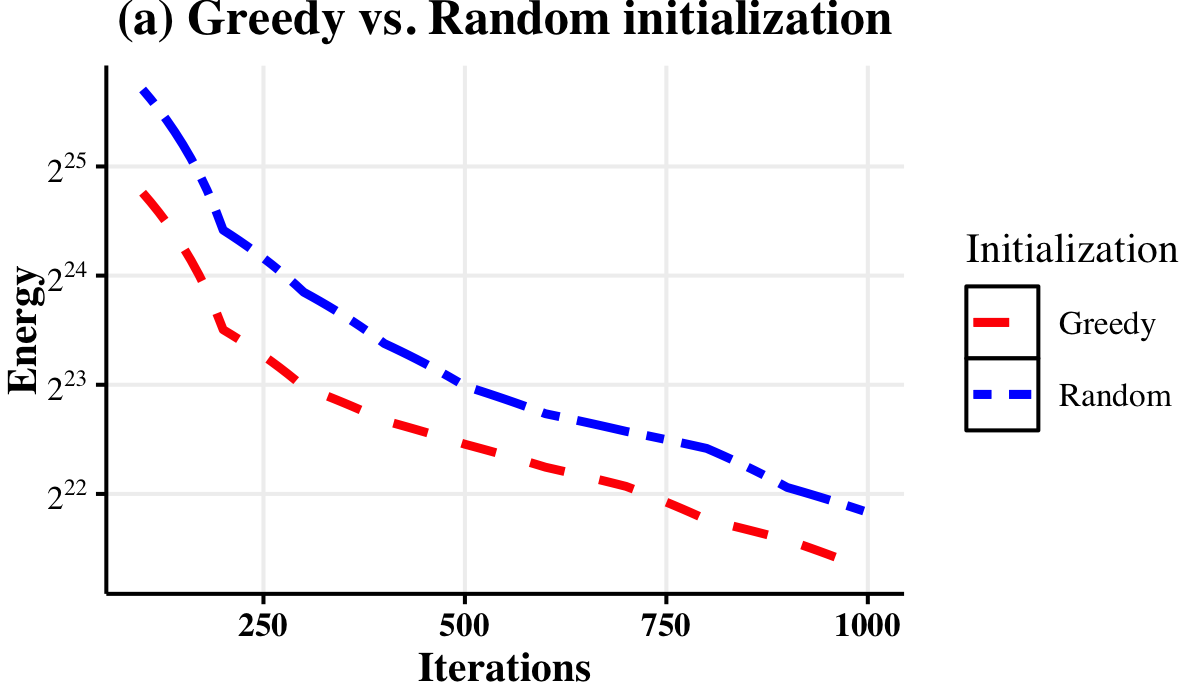
\includegraphics[width=0.33\linewidth]{figures/initialization.png}
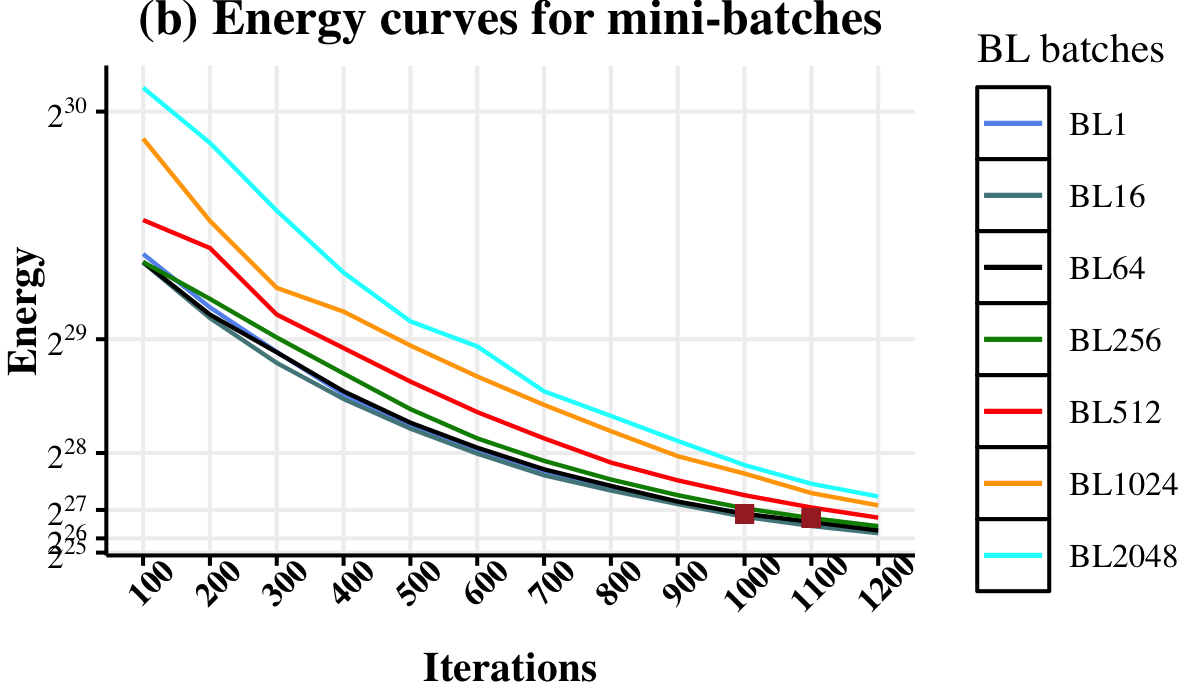
\includegraphics[width=0.33\linewidth]{figures/batchesenergy3.png}
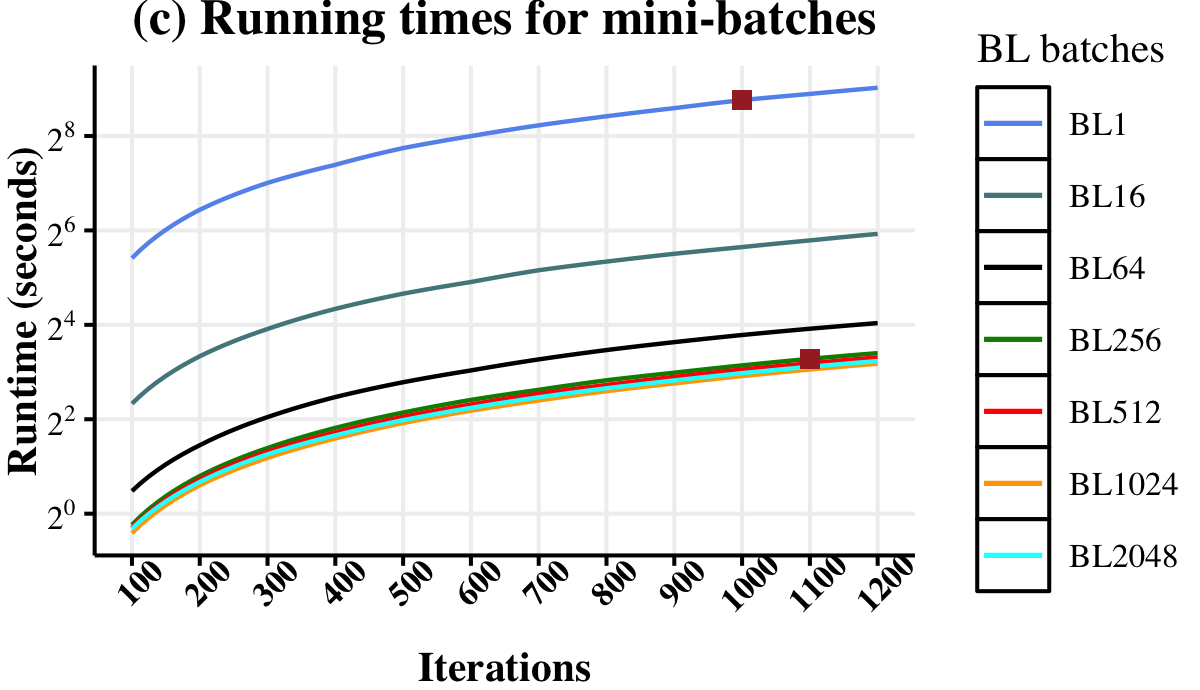
\includegraphics[width=0.33\linewidth]{figures/batchesruntime3.png}
\vspace{-0.4cm}
\caption{(a) Energy curves for greedy and random initialization (\emph{3elt\_dual} graph). (b) Energy curves ($\log$ scale) for different batches (\emph{pkustk02} graph). (c) Running time ($\log$ scale) for different batches of \toolname{} (\emph{pkustk02} graph).}
\label{fig:selfcheckout}
\end{figure*}
%\vspace{-0.3cm}

\subsubsection{Number of threads} 
Using more threads not necessarily translates to faster runtime, especially for small graphs.
This is because of the overhead of thread \emph{fork-join} model used in OpenMP.
For larger graphs with more than 100,000 vertices, we recommend employing all available threads.
For smaller graphs, users can consider using fewer threads. 
Hence, the number of threads is provided as an option in \toolname.

%It is recommended 
%Choosing a higher number of threads does not always perform well especially when the graph has few number of vertices. This is mainly due to the overhead of thread \emph{fork-join} model. We restrict such unnecessary overhead by choosing a suitable value for threads. For \toolnameBH{}, we allow more than 32 threads in the default setting when number of vertices in the graph is more than one million; however, user can always reset the default value.
% AA: It is not good to say 32 or any number here because it will be specific for Skylake machine that we are using.

\begin{figure*}[ht]
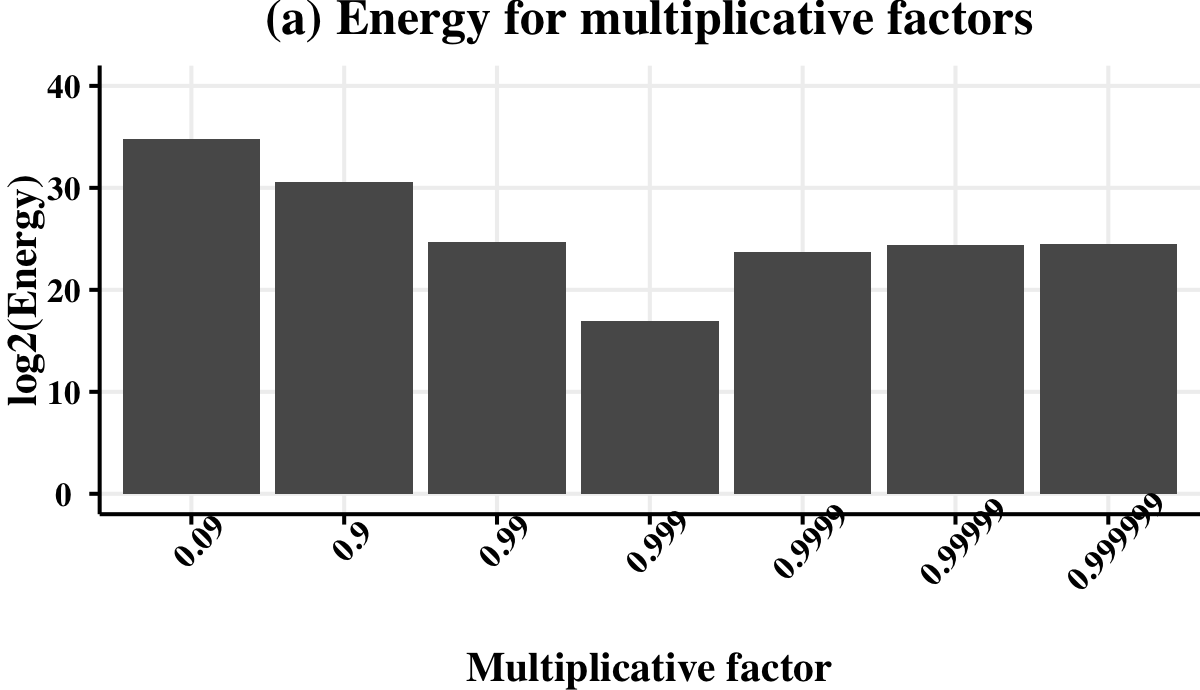
\includegraphics[width=0.33\linewidth]{figures/tvalues.png}
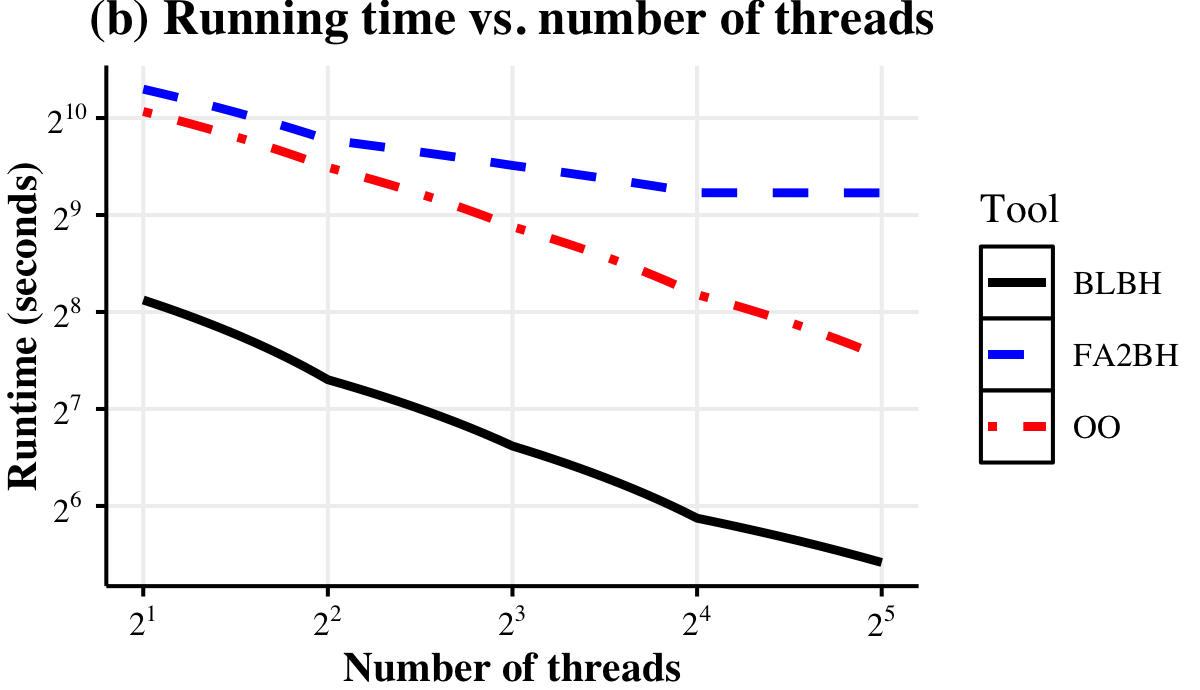
\includegraphics[width=0.33\linewidth]{figures/strongs.png}
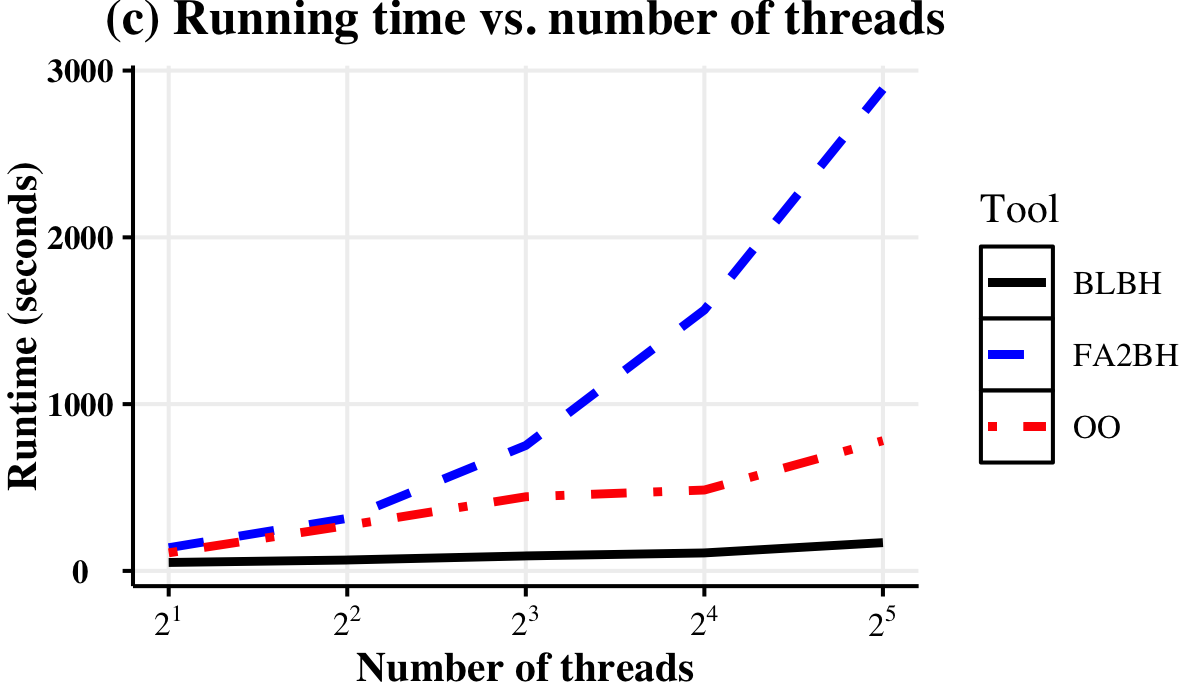
\includegraphics[width=0.33\linewidth]{figures/weaksrev.png}
\vspace{-0.4cm}
\caption{(a) Energy values ($\log$ scale) for different multiplicative factor of $Step$ using \emph{3elt\_dual} graph. (b) \commentKhaled{Strong scaling: Running time ($\log$ scale) for different number of threads using a synthetic graph of $2^{18}$ vertices generated by \cite{lancichinetti2008benchmark}. (c) Weak scaling: Running time (seconds) for different number of threads and graph sizes.}}
\vspace{-0.5cm}
\label{fig:selfcheckout2}
\end{figure*}

\subsubsection{Step length or learning rate}
Line 14 of Algorithm~\ref{euclid} uses a multiplicative factor for $Step$, which dictates both convergence and the quality of the final layout.
Intuitively, we want to adapt the step length so that the algorithm takes bigger steps in the beginning but increasingly smaller steps as we move closer to the minimum energy.
Fig.~\ref{fig:selfcheckout2}(a) shows layout energies at convergence with various multiplicative factors for the \emph{3elt\_dual} graph.
%Here, a multiplication factor of 0.9 means that we reduce the step size by $10\%$ in every iteration.
We observe that the factor of 0.999 (that is $0.1\%$ reduction of step length in every iteration) provides the best balance as the converged energy is minimum for this factor. 
Hence, we use this multiplicative factor in all experiments with \toolname{}.
We note that adaptive steps are also used in other force-directed layouts such as in the algorithm developed by Yifan Hu~\cite{hu2005efficient}.
In this paper, we empirically identify an effective adaption policy so that \toolname{} converges faster.

%\subsubsection{Multiplicative factor of step length}
%In Algorithm \ref{euclid}, notice in line 14 that there is a multiplicative factor for $Step$. Different tool uses different technique for updating step size. For example, Yifan Hu \cite{hu2005efficient} used 0.9 and an adaptive update technique. In our tool, we select this multiplicative factor empirically based on convergence speed for different graphs. We show experimental results of multiplicative factor on \emph{3elt\_dual} graph in Fig.~\ref{fig:selfcheckout2}(a). We notice that if we increase this value from $0.09$, Energy decreases and when we reach $0.999$, Energy reaches to a minimal value. After that Energy increases with the increase of multiplicative factor. %A concrete theory may play important role for explanation to this characteristic which is beyond of this paper. For all of our further experiments, we use this multiplicative factor in all versions of \toolname{}.

\subsection{Running Time and Scalability}
\label{lab:runtime}
We run all algorithms for 500 iterations using 47 threads (one thread per core) and report their runtime in Table~\ref{tab:runningtime}.
Since OpenOrdG leaves out a core for kernel-specific tasks, we also leave a core unutilized for fairness in comparison.  
In Table \ref{tab:runningtime}, we include time for all steps except file input/output operations.
If we consider exact force calculations, \toolname{} is on average $15\times$ faster than ForceAtlas2 (min:$7.6\times$, max:$21.8\times$).
For approximate force calculation, \toolnameBH{} is on average $2\times$ faster than OpenOrd (min:$1.4\times$, max:$9.5\times$).
Both \toolnameBH{} and OpenOrd are faster than ForceAtlas2BH.
Notice that OpenOrdG (that is Gephi's OpenOrd) also runs fast, but its layout quality is very low as seen in the next section.
Overall, \toolnameBH{} is almost always the fastest algorithm as denoted by bold numbers in Table \ref{tab:runningtime}.
We also tested tsNET~\cite{kruiger2017graph} to conduct some experiments (with perplexity and learning rate set to 800 and 6000, respectively). 
We observe that tsNET can generate good layouts for small graphs, but failed to generate any layout for medium or bigger graphs in our experiments. 
For small graphs like \emph{3elt\_dual}, tsNET took around 1 hour whereas other multi-threaded tools generated layout within few seconds. 
Hence, we did not include tsNET runtimes in Table \ref{tab:runningtime}. 

{\bf Thread and vertex scalability.} We now discuss the thread and vertex scalability of the three fastest algorithms: \toolnameBH{} (FLBH), ForceAtlas2BH (FA2BH), and OpenOrd (OO).
As discussed in section \ref{lab:datasets}, we use a benchmark tool~\cite{lancichinetti2008benchmark} to generate graphs for the scalability experiment.
Fig.~\ref{fig:selfcheckout2}(b) shows the thread scalability for a graph with $2^{18}$ vertices.
We observe that both  \toolnameBH{}  and OpenOrd scale linearly with threads (cores), but  \toolnameBH{} is $\sim4\times$ faster than OpenOrd on all thread counts. 
ForceAtlas2BH does not scale linearly, and it is generally not faster than OpenOrd.
Fig.~\ref{fig:selfcheckout2}(c) shows the \commentKhaled{weak scalability where we use increasingly larger graphs varying number of threads. Fig.~\ref{fig:selfcheckout2}(c) starts with a graph of $2^{16}$ vertices running on 2 threads. Then, we increasingly double the problem size as well as computing resource, run experiments and report the runtime. Among all three algorithms, we observe that \toolnameBH{}'s work distribution remains balanced (i.e., curve remains horizontal). Hence, \toolnameBH{} shows superior weak scaling performance compared to other two algorithms.}

{\bf Memory usage.} We measured the memory consumption of all algorithms using the {\myfont memory-profiler} python package.
For the lxOSM graph, \toolname{}, \toolnameBH{}, ForceAtlas2, ForceAtlas2BH, OpenOrdG, and OpenOrd consumed maximum memory of 16.36MB, 30.34MB, 676.38MB, 1348.38MB, 1265.32MB and 14.12MB, respectively. 
Gephi's ForceAtlas2, ForceAtlas2BH and OpenOrdG consumed higher memory than others possibly because of the high memory requirements of Gephi itself.
In fact, ForceAtlas2BH failed to generate layouts for two large graphs due to its high memory consumption.
In our algorithm, Barnes-Hut force approximation requires additional space to store the quad-tree data structure, and hence it consumed more memory than the exact force computation. 
Overall, \toolnameBH{} can compute layouts faster without consuming significant memory. 


%For this experiment, we run all tools for 500 iterations using 47 threads\footnote{For this experimental setup, we choose 47 because of OpenOrdG which by default obliges to use one less core than maximum available cores} and results are reported in Table \ref{tab:runningtime}. We measure running time of all tools for initialization and iterative optimization steps which excludes file input/output operations. In Table \ref{tab:runningtime}, we see that either \toolname{} or \toolnameBH{} is winner in all cases and it clearly indicates robustness of our algorithm compared to all other tools. For example, ForceAtlas2BH (FA2BH) takes 46.98 seconds for \emph{finan512} graphs whereas \toolnameBH{} takes only 10.53 seconds. For the same graph, multi-threaded version of OpenOrdG and OpenOrd take around 31.74 and 22.57 seconds, respectively. Notice that OpenOrdG also runs fast but we see later that the quality of layout is not good. Among all, Barnes-Hut version of our introduced \toolname{} is the fastest tool and generate good quality layout. Note that we do not report running time of tsNET as it could not generate layout for all graphs using our computing resources (even for \emph{finance256} graph, tsNET failed to generate layout). For small graph like \emph{3elt\_dual}, tsNET took around 1 hour whereas other multi-threaded tools generate layout within few seconds. So, we skipped tsNET for further experiments as high performance is our focus in addition to good quality layout. 

%We also tested the memory usage by all tools using {\myfont memory-profiler} python package and observed that \toolname{}, \toolnameBH{}, ForceAtlas2, ForceAtlas2BH, OpenOrdG and OpenOrd consumed maximum memory of 16.36MB, 30.34MB, 676.38MB, 1348.38MB, 1265.32MB	and 14.12MB, respectively, for lxOSM graph. Note that Gephi's ForceAtlas2, ForceAtlas2BH and OpenOrdG consumed higher memory than others whereas our tool consumed significantly less memory to produce high quality layouts within very short time. In fact, for this high memory consumption, ForceAtlas2BH failed to produce layout for two big graphs using our computing resources. Barnes-Hut force approximation requires additional space to store quad-tree and hence consumed more memory than $O(n^2)$ version. In summary, \toolname{} and/or \toolnameBH{} perform well for efficient cache memory usage and processing vertices of a batch in parallel. 




%We also show the scalability of \toolnameBH{} (BLBH), FA2BH and OpenOrd (OO) in Figs.~\ref{fig:selfcheckout2}(b) and \ref{fig:selfcheckout2}(c). All experimental setups are same as before. As discussed in section \ref{lab:datasets}, we use a benchmark tool by Lancichinetti et al. \cite{lancichinetti2008benchmark} to generate all graphs for this experiment. In Fig.~\ref{fig:selfcheckout2}(b), we show run time using different number of threads on a graph of $2^{18}$ vertices. We see that \toolnameBH{} is faster than other tools and almost linearly scalable over different number of threads. Our experiments also show that OpenOrd is scalable and faster than ForceAtlas2BH. In Fig.~\ref{fig:selfcheckout2}(c), we show scalability over different size of graphs using 32 threads for each tool. We observe that run time increases linearly for all tools.

\begin{table}[!tb]
\caption{Runtime for different methods. Lower value represents better result. BL, BLBH, FA2, FA2BH, OOG and OO represent \toolname{}, \toolnameBH{}, ForceAtlas2, ForceAtlas2BH, OpenOrdG and OpenOrd, respectively. Better results are shown in bold font.}
\vspace{-4pt}
\centering
\begin{tabular}{|p{1.2cm}|p{0.63cm}|p{0.6cm}|p{0.65cm}|p{0.7cm}|c|p{0.8cm}|}
\hline
\multirow{2}{*}{\textbf{Graph}} & \multicolumn{6}{c|}{\textbf{Running time (seconds)}} \\ \cline{2-7} 
                                & BL   & BLBH   & FA2   & FA2BH   & OOG   & OO  \\ \hline
Powergrid	    &   \textbf{0.95}	&   0.98	&   20.73	&   3.04	&   1.67 & 1.43\\ \hline
add32	&   1.03	&   \textbf{1.02}	&   20.75	&   3.15	&   1.71 &   1.45 \\ \hline
ba\_network	&   1.42	&   \textbf{1.22}	&   25.47	&   3.61	&   2.18 & 1.78 \\ \hline
3elt\_dual	&   2.92	&   \textbf{1.54}	&   54.6	&   4.87	&   3.17 & 2.67 \\ \hline
PGP	&   4	&   \textbf{1.83}	&   68.67	&   6.26	&   4.18 & 3.26\\ \hline

pkustk02	&   4.23	&   \textbf{1.98}	&   76.69	&   10.72	&   10.32 & 3.83 \\ \hline
fe\_4elt2	&   4.33	&   \textbf{1.86}	&   75.4	&   6.34	&   4.21 & 3.35 \\ \hline
bodyy6	&   12.3	&  \textbf{2.95}	&   143.08	&   9.69	&   6.75 & 5.85 \\ \hline
pkustk01	&   16.23	&   \textbf{3.43}	&   242.72	&   18.49	&   15.33 & 7.25 \\ \hline
OPF\_6000	&   29.75	&   \textbf{4.69}	&   266.96	&   18.31	&   12.45 & 8.95\\ \hline
finance256	&   45.49	&   \textbf{5.4}    &   412.6	&   20.37	&   14.69 & 11.18\\ \hline
finan512	&   185.8	&   \textbf{10.53}	&   1408	&   46.98	&   31.74 & 22.57\\ \hline
lxOSM	&   -	&   \textbf{21.59}	&   -	&  72.30 	&  -  & 33.62 \\ \hline
comYout.	&   -	&   \textbf{174.5}	&   -	&   1504.7	& -    & 1670.52 \\ \hline
%af\_shell10	&   -	&   \textbf{221.27}	&   -	&   -	&  -  & 508.55\\ \hline
Flan\_1565	&  -	&   \textbf{224.3}	&   -	&   -	&   - & 609.56 \\ \hline
\end{tabular}
\label{tab:runningtime}
\vspace{-0.4cm}
\end{table}




\begin{table*}[!t]
\centering
\caption{Layouts of different graphs generated by different algorithms. BatchLayout convergence criteria was set to 1E-6. Number of iterations and running time are shown in supplementary file, Table S2.}
\label{tab:convergedlayouts}

\begin{tabular}{|c|p{2.5cm}|p{2.6cm}|p{2.6cm}|p{2.6cm}|p{2.5cm}|}
\hline
\textbf{Graph}   & \textbf{BatchLayout} & \textbf{BatchLayoutBH} & \textbf{ForceAtlas2} & \textbf{ForceAtlas2BH} & \textbf{OpenOrd} \\ \hline
        \textbf{Powergrid} & \multicolumn{5}{|c|}{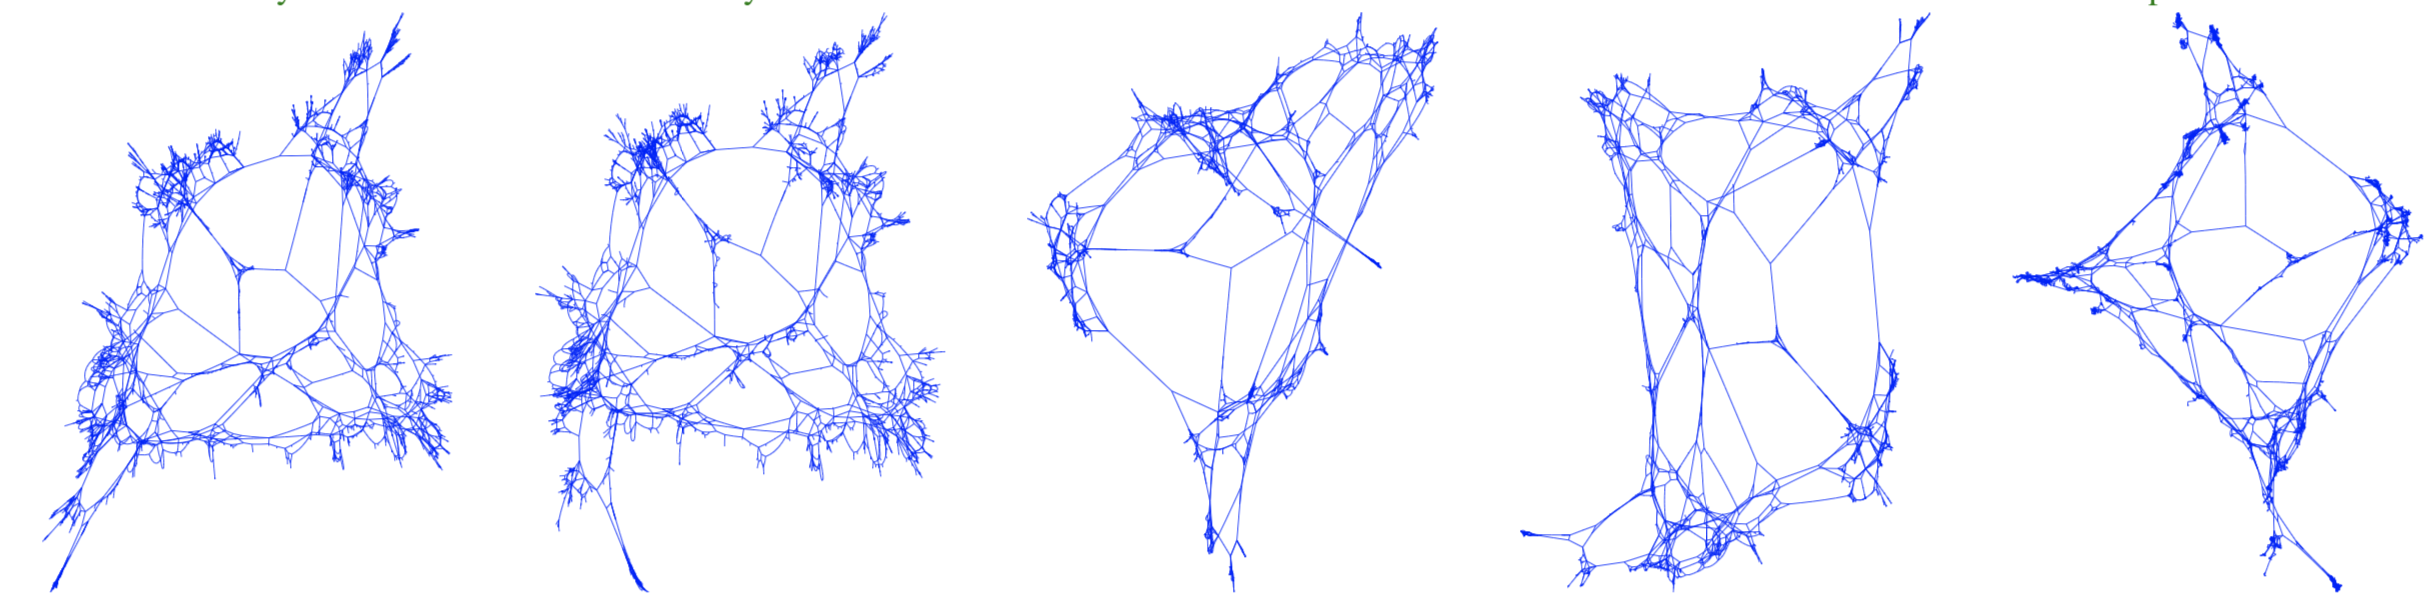
\includegraphics[height=1.8cm,width=0.8\linewidth]{layouts/convergedlayouts/us_powergrid_converged.png}}                                                                                                                \\ \hline

\textbf{ba\_network}        & \multicolumn{5}{c|}{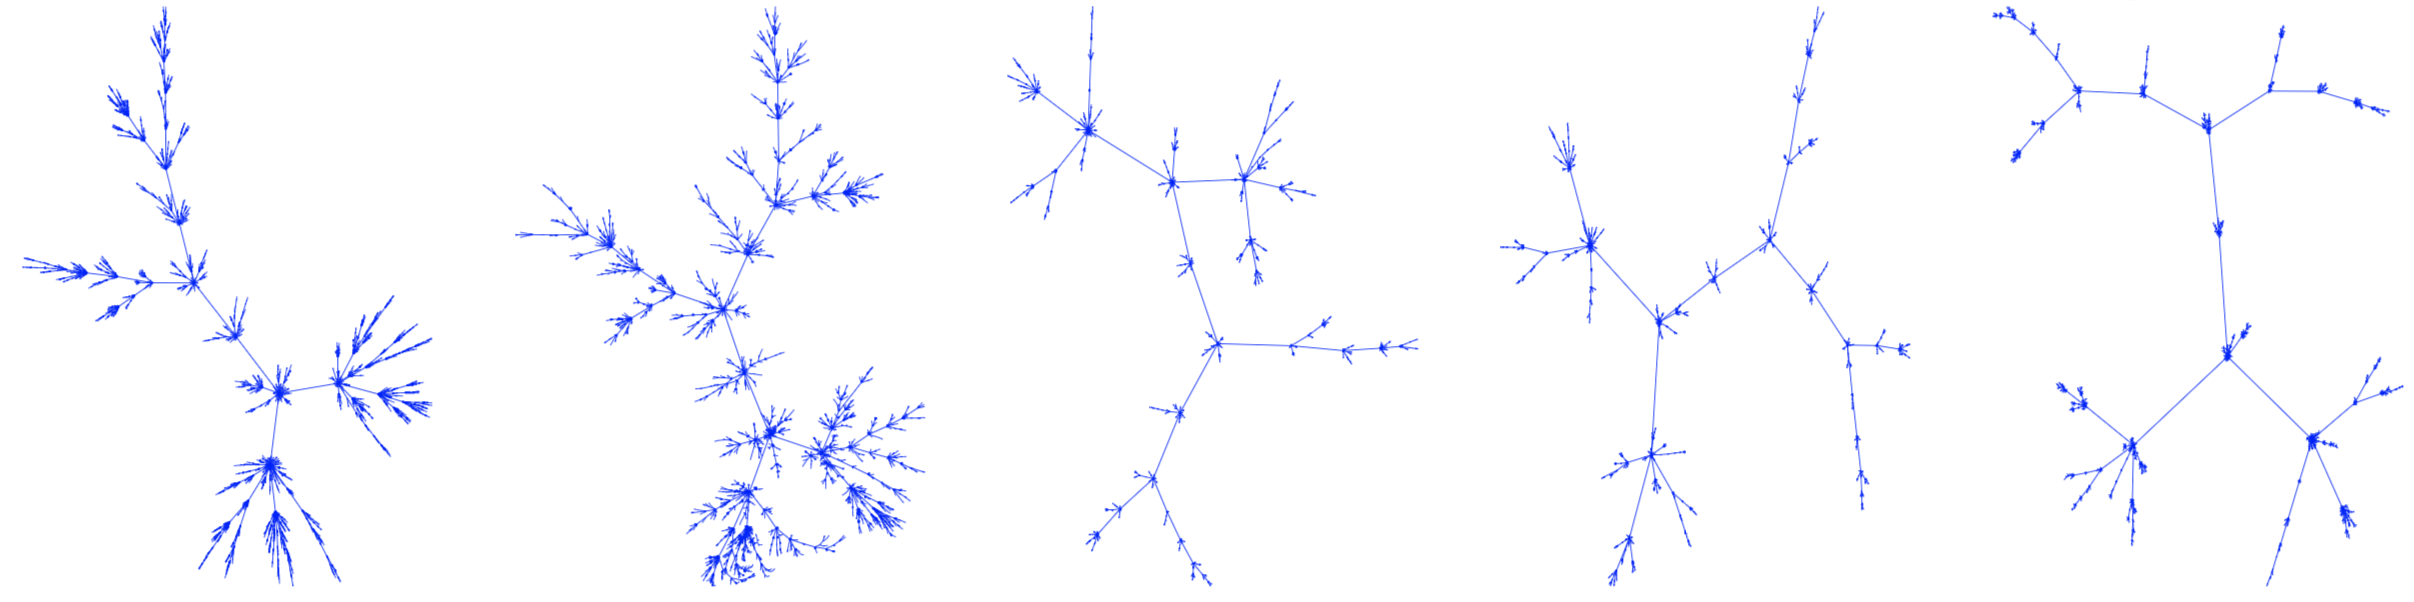
\includegraphics[height=1.8cm,width=0.8\linewidth]{layouts/convergedlayouts/ba_network_converged.png}}                                                                                                                 \\ \hline
\textbf{3elt\_dual}        & \multicolumn{5}{c|}{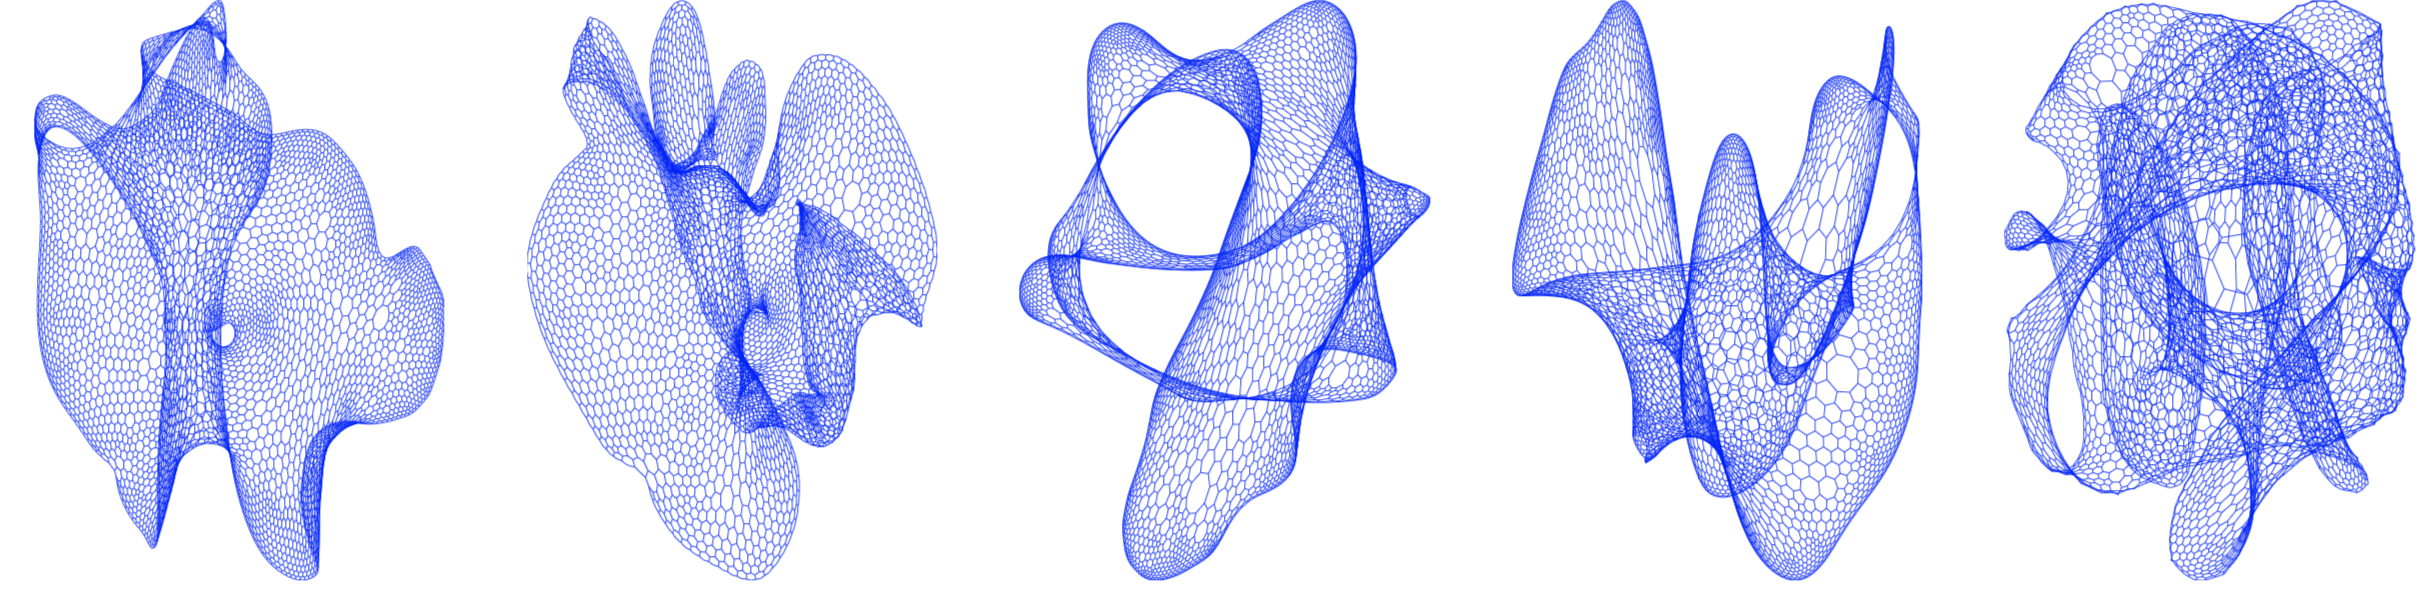
\includegraphics[height=1.8cm,width=0.8\linewidth]{layouts/convergedlayouts/3elt_dual_converged.png} }                                                                                                                                                        \\ \hline
\textbf{pkustk02}        & \multicolumn{5}{c|}{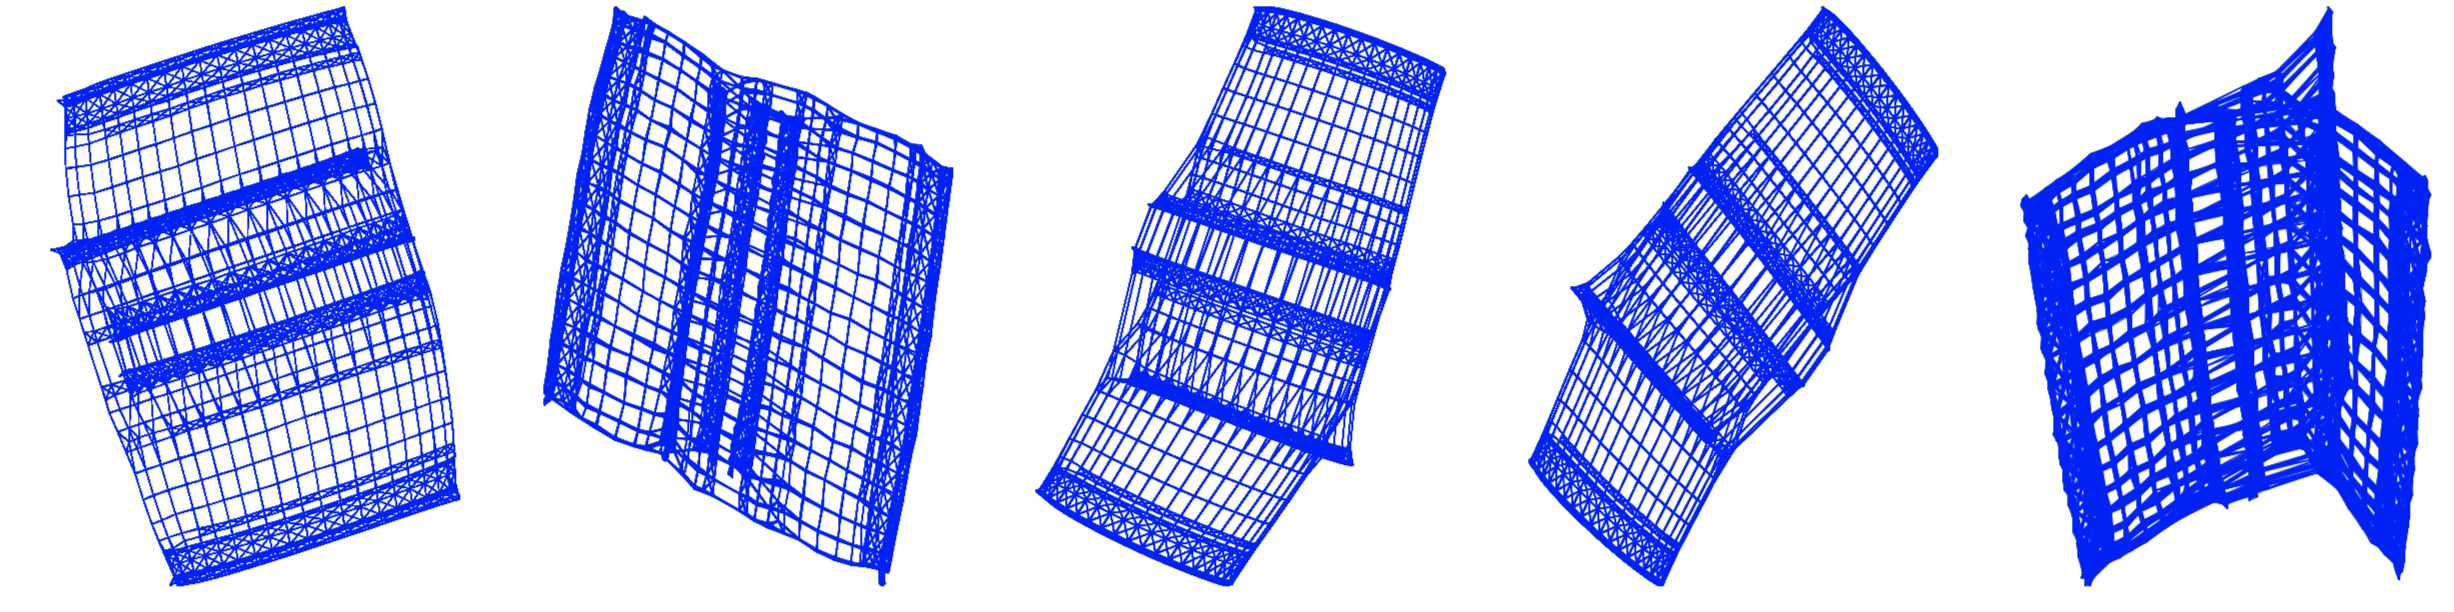
\includegraphics[height=1.8cm,width=0.8\linewidth]{layouts/convergedlayouts/pkustk02_converged.png}}                                                                                                                 \\ \hline
\textbf{fe\_4elt2}        & \multicolumn{5}{c|}{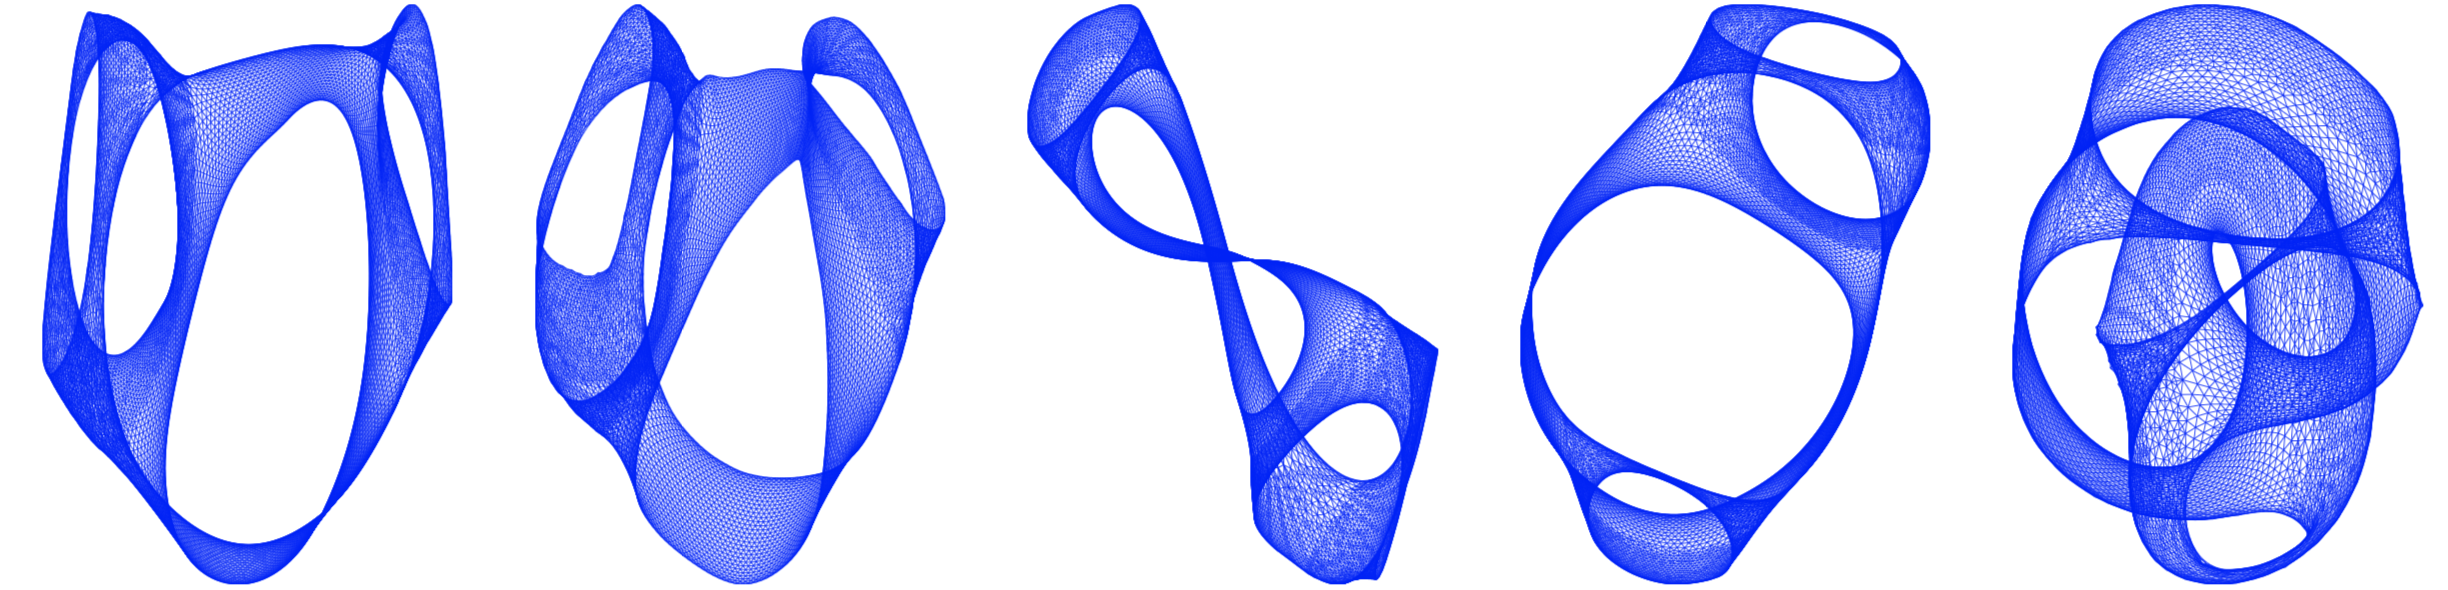
\includegraphics[height=1.8cm,width=0.8\linewidth]{layouts/convergedlayouts/fe_4elt2_converged.png}}                                                                                                                 \\ \hline
\textbf{bodyy6}        & \multicolumn{5}{c|}{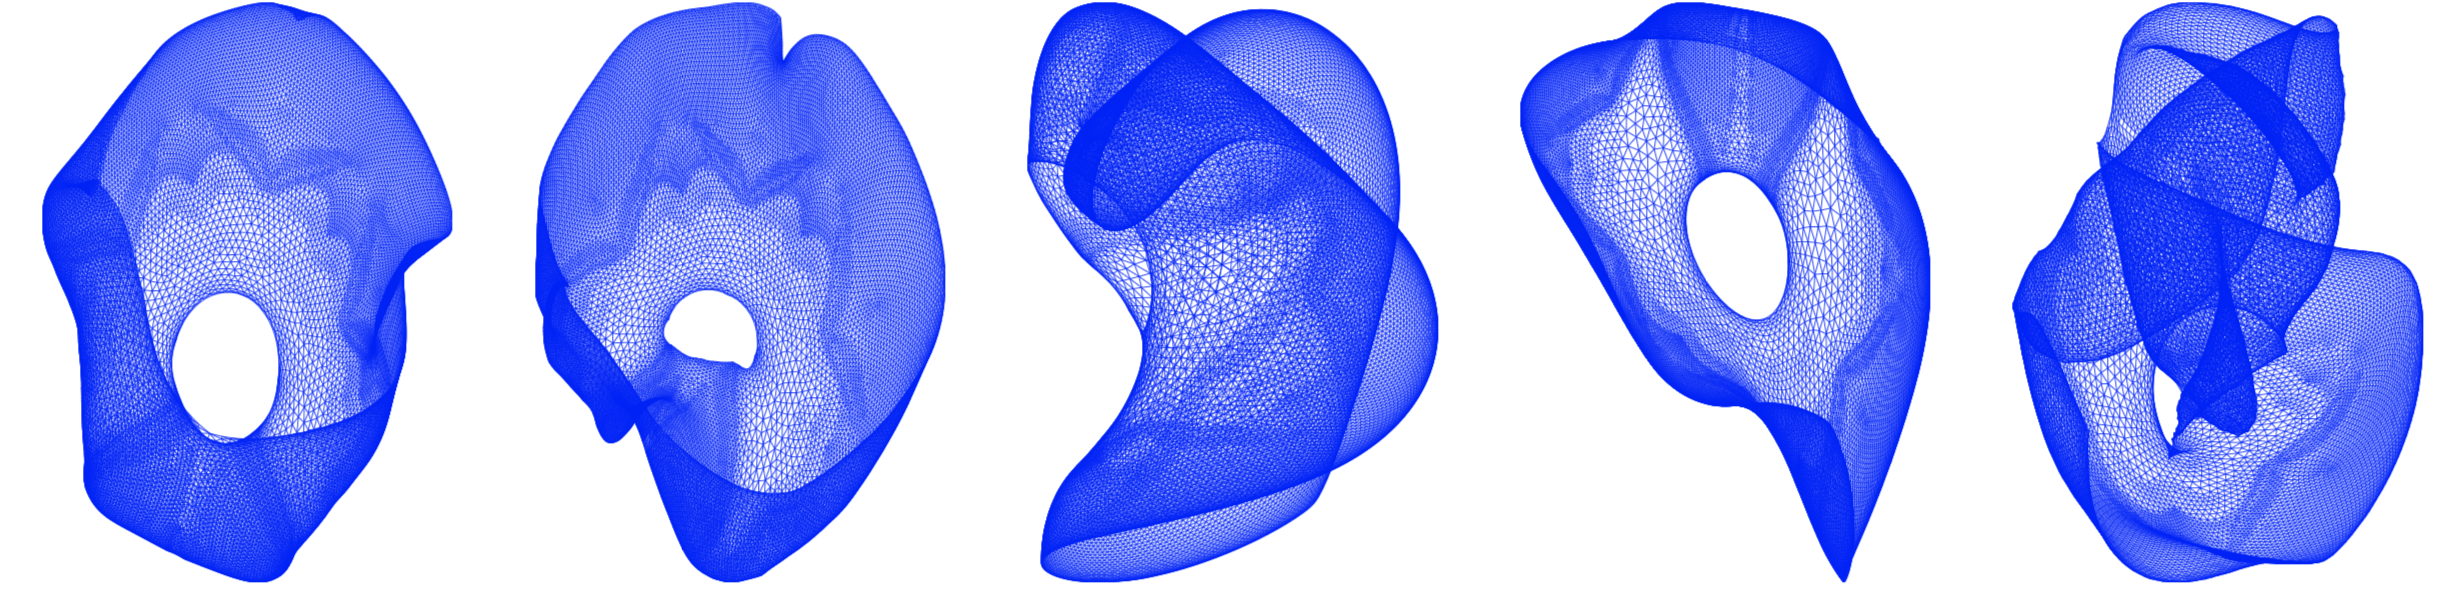
\includegraphics[height=1.8cm,width=0.8\linewidth]{layouts/convergedlayouts/bodyy6_converged.png}}                                                                                                                 \\ \hline

\textbf{pkustk01}        & \multicolumn{5}{c|}{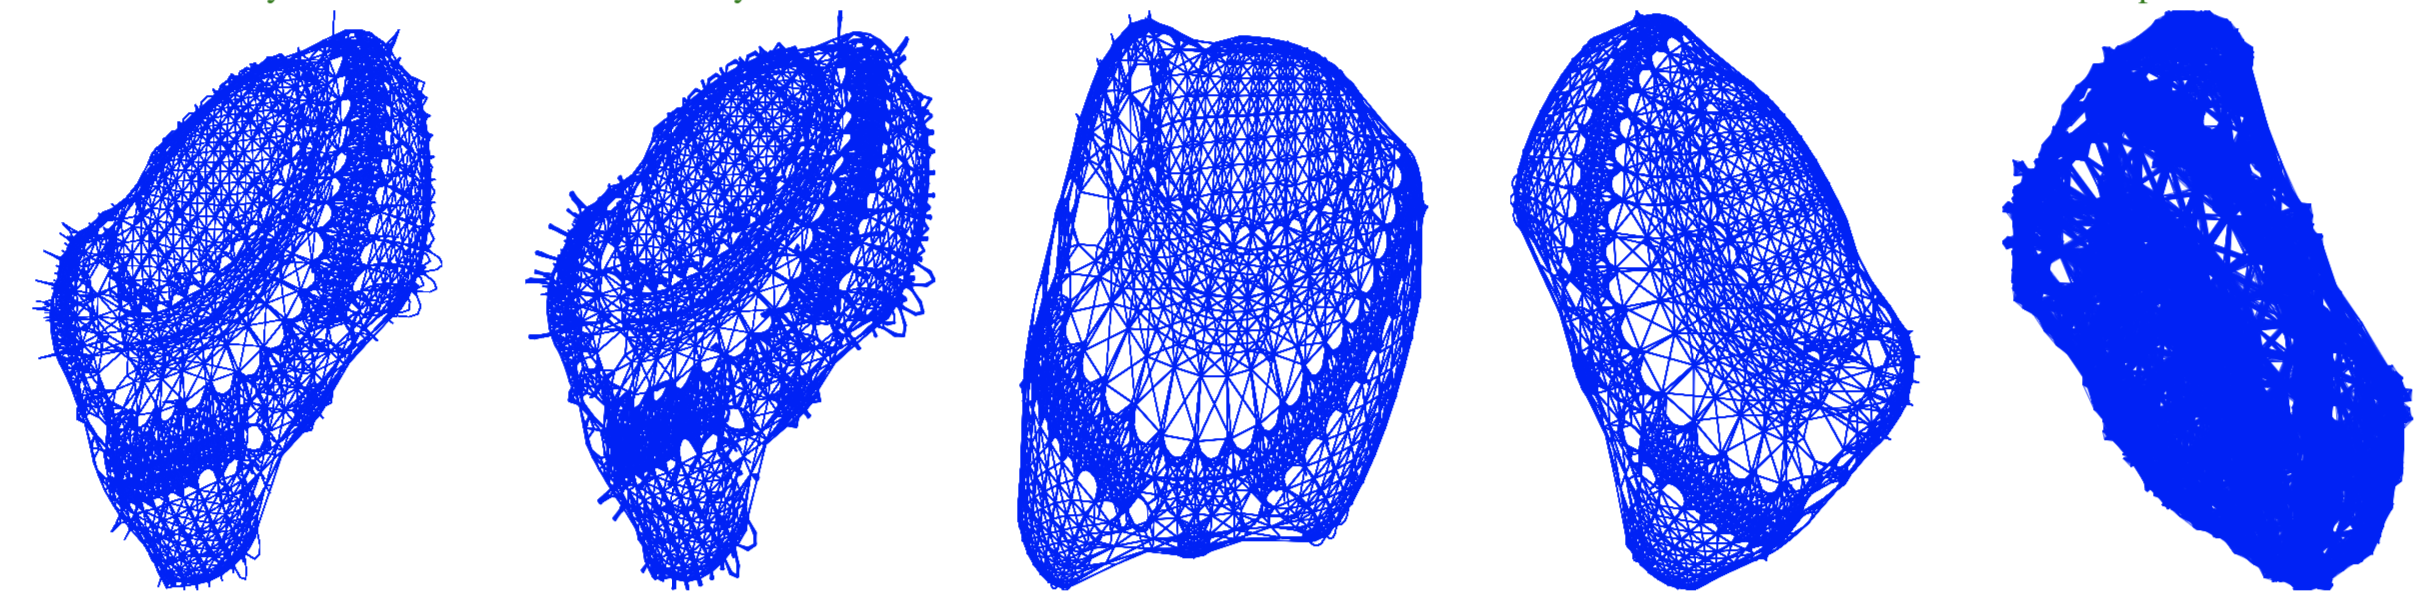
\includegraphics[height=1.8cm,width=0.8\linewidth]{layouts/convergedlayouts/pkustk01_converged.png}}  \\ \hline

\textbf{finan256}        & \multicolumn{5}{c|}{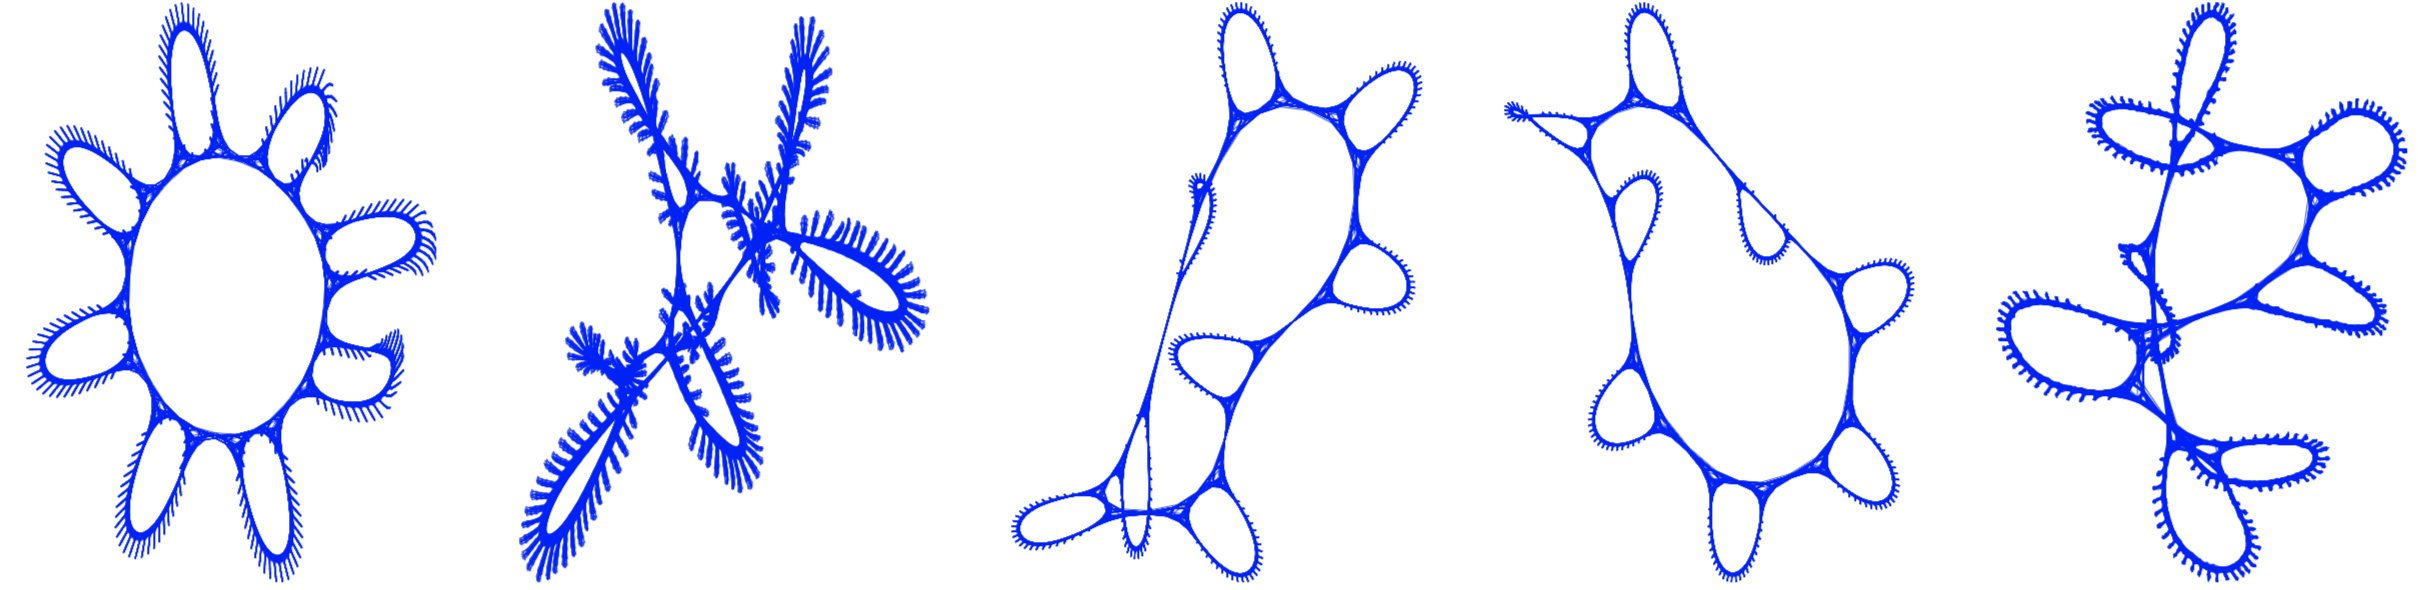
\includegraphics[height=1.8cm,width=0.8\linewidth]{layouts/convergedlayouts/finan256_converged.png}}  \\ \hline
\end{tabular}
\vspace{-0.2cm}
\end{table*}

\subsection{Visualization}
We now visualize the layouts generated by all algorithms considered in the paper. 
At first, we run \toolname{} until convergence (when the energy difference between successive iterations becomes less than $10^{-6}$).
Then, all other algorithms including \toolnameBH{} were run for the same number of iterations that \toolname{} took to converge.
The visualization from these layouts are shown in Table~\ref{tab:convergedlayouts}.
The runtime and converged energy are provided  in supplementary Table S2, which shows that \toolnameBH{} runs much faster than other tools.
Table~\ref{tab:convergedlayouts} demonstrates that \toolname{} and \toolnameBH{} produce \commentKhaled{readable} layouts that are comparable or better than ForceAtlas2 and ForceAtlas2BH, respectively.
Generally, \toolnameBH{} and ForceAtlas2BH layouts are much better than OpenOrd.
Gephi's OpenOrd generates inferior layouts; hence, we did not show them in Table~\ref{tab:convergedlayouts}.
Note that \toolname{} uses Fruchterman and Reingold as its default energy model, which is different from the default model in ForceAtlas2. 
Hence, \toolname{}'s superior layouts for some graphs (e.g., finan256) are not surprising because the FR model usually generates better layouts as was also reported in the ForceAtlas2 paper~\cite{jacomy2014forceatlas2}.
ForceAtlas2 does not use FR as its default model possibly because of its higher computational cost (also reported in ~\cite{jacomy2014forceatlas2}).
In this paper, we show that the FR algorithm runs much faster in our \toolname{} framework and can generate better layouts for some graphs. 

In the scalability and runtime experiments, we showed results with a fixed 500 iterations. %(per iteration runtime is usually fixed for an algorithm). 
Supplementary Table S1 shows the visualization from all algorithms after 500 iterations.
In many cases, layouts after 500 iterations are close to the layouts at convergence. 
Hence, many algorithms including \toolname{} provide ``number of iterations" as an option to users.   

Both \toolname{} and ForceAtlas2 provide many options beside default options used in our experiments. 
It is possible that tuning these parameters will generate better-quality layouts for some graphs.
However, we stick to default parameters in this paper for simplicity and fairness. 
OpenOrd may generate different layouts for the same graph when different numbers of threads are used.
By contrast, \toolname{} and \toolnameBH{} generate the same layout for a given graph irrespective of number of threads. 


\begin{figure}[!t]
\vspace{-0.1cm}
    \centering
    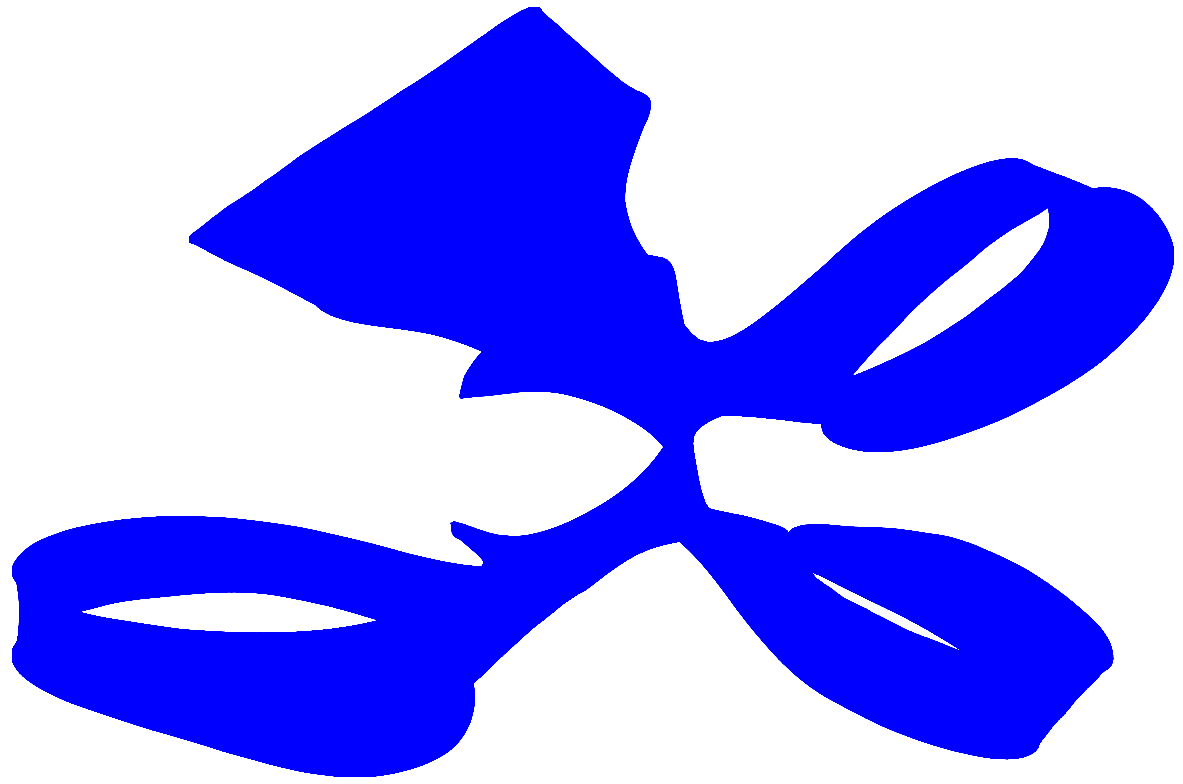
\includegraphics[width=0.48\linewidth]{layouts/FLan_BatchLayoutBH_5000.png}
    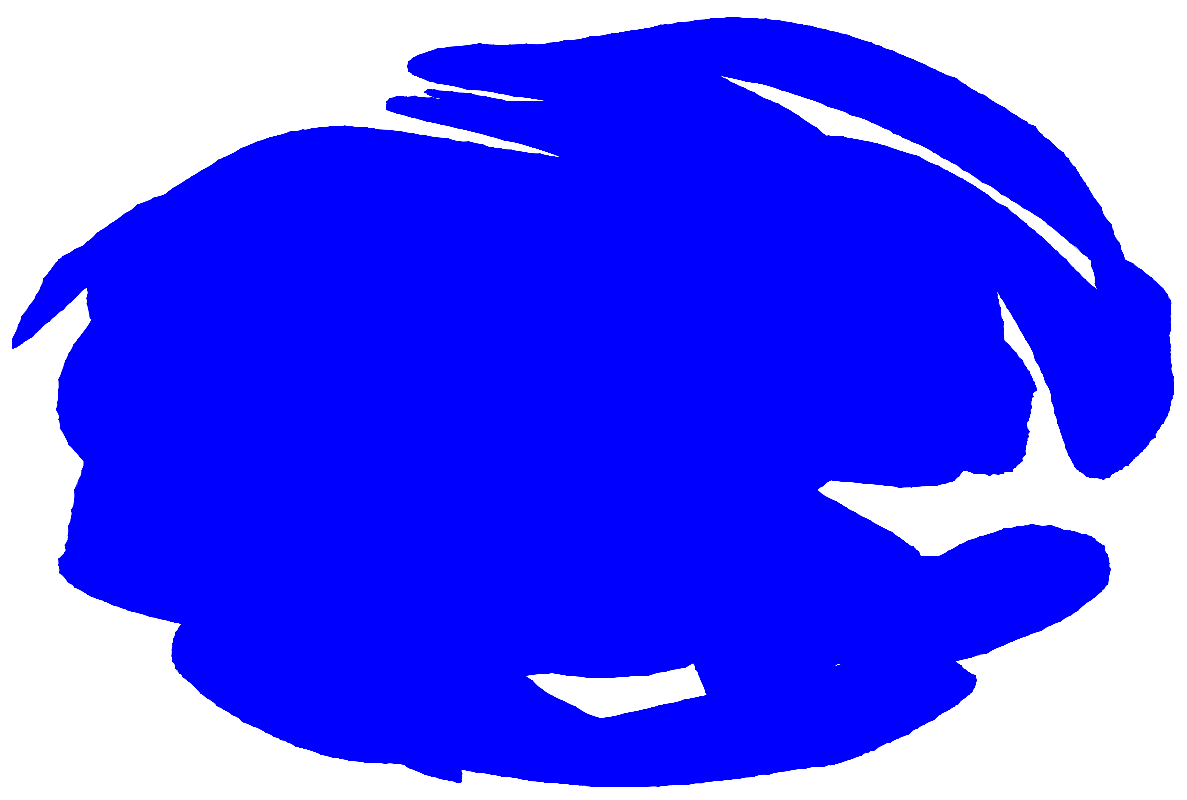
\includegraphics[width=0.48\linewidth]{layouts/Flan_OpenOrd_5000.png}
    \caption{Layouts of \emph{Flan\_1565} graph (1.56M vertices and 114.2M edges) generated by \toolnameBH{} (left) and
    OpenOrd (right).
    %Layouts of Flan\_1565 which has around 1.56M vertices and 114.2M edges. We ran each tool for 5000 iterations to generate layout. \toolnameBH{} (left subfigure) took only 49 minutes to generate high quality layout whereas OpenOrd (right subfigure) took around 1 hour and 39 minutes though quality of layout is very poor. ForceAtlas2BH failed to allocate memory in our computing machine for this graph and could not generate any layout. \toolnameBH{} generates high quality layout in shortest possible time.
    }
    \vspace{-0.4cm}
    \label{fig:verybiggraph}
\end{figure}

Finally, Fig.~\ref{fig:verybiggraph} shows the layout of \emph{Flan\_1565}, the largest graph in our dataset.
We show layouts from \toolnameBH{} and OpenOrd after running them for 5000 iterations (ForceAtlas2BH went out of memory for this graph).
For this graph,  OpenOrd's layout is not good enough even though we allow both algorithms to run for 5000 thousands of iterations. 
Furthermore, OpenOrd took 1 hour and 39 minutes whereas \toolnameBH{} took 49 minutes to finish 5000 iterations. 
This clearly demonstrates the effectiveness of \toolnameBH{} to visualize graph with hundreds of millions of edges.
However, generating layouts in half an hour may not be good enough for certain applications.
We plan to address this by implementing  \toolnameBH{} for distributed systems.
%and for GPUs. 


%We show visualization of all layouts in supplementary file, Table S1, for which we compared aesthetic measures. We see that \toolname{} and \toolnameBH{} generate better or competitive layouts for all graphs. Note that we select batch size as 256 which is suitable for big graphs but for small graphs we can select smaller batch size as it will not increase running time much but generate very good quality layouts. Actually, more better quality layouts are achievable by tuning several hyper parameters of \toolname{} and \toolnameBH{} which is a trade-off between running time and quality. For simplicity of explanation we used same hyper parameters for all graphs. We also notice that there is significant difference between OpenOrdG and original OpenOrd. When we observe this, we include both implementations in our experimental results for the sake of clarification. From layouts, we can conclude that OpenOrd is more appropriate to compare results than OpenOrdG though it offers more flexibility. As stated by authors, one drawback of OpenOrd is that it generates different layouts if we use different number of threads which is not aligned with scientific computation. Our \toolname{} and \toolnameBH{} generate same layout and report same energy value for different number of threads. 

%We provide converged layouts of \toolname{} in Table \ref{tab:convergedlayouts} based on a threshold value of $10^{-6}$. All other tools including \toolnameBH{} were run for same number of iterations that \toolname{} took to converge. We provide this information along with runtime in supplementary file, Table S2, where we see that \toolnameBH{} runs much faster than other tools. In Table \ref{tab:convergedlayouts}, we also observe that \toolnameBH{} produces high quality layout which proves its effectiveness along with better running time.



% Finally, we generate layout of \emph{Flan\_1565} graph for 5000 iterations using 48 threads and report layouts in Fig. \ref{fig:verybiggraph}. Note that ForceAtlas2BH failed to allocate heap memory in our computing machine for this big graph and thus could not generate any layout. Observe that \toolnameBH{} generates high quality layout within the smallest possible time than OpenOrd which clearly indicates effectiveness and efficacy of \toolnameBH{} for big graphs.

\begin{table*}[!t]%[t]
\caption{Comparison of Stress (ST) and Neighborhood preservation (NP) measures among all tools. For ST, a lower value means a better result and for NP, a higher value represents a better result. Better results are shown in bold font.}
\vspace{-4pt}
\centering
\begin{tabular}{|c|c|c|c|c|c|l|c|c|c|c|c|c|}
\hline
\multirow{2}{*}{\textbf{Graph}} & \multicolumn{6}{c|}{\textbf{ST}}                            & \multicolumn{6}{c|}{\textbf{NP}}            \\ \cline{2-13} 
                                & BL       & BLBH     & FA2       & FA2BH & OO & OOGH & BL & BLBH & FA2 & FA2BH & OOG & OO \\ \hline

Powergrid	&	\textbf{1.3E+6}	&	1.6E+6	&	2.4E+6	&	2.2E+6	&	2.5E+6	&	2.4E+6	&		0.39	&	0.266	&	0.403	&	\textbf{0.408}	&	0.324	&	0.336 \\ \hline

add32	&	2.2E+6	&	\textbf{1.9E+6}	&	5.3E+6	&	5.4E+6	&	6.2E+6	&	2.3E+6	&			0.453	&	0.347	&	\textbf{0.538}	&	0.523	&	0.362	&	0.409 \\ \hline

ba\_network	&	2.8E+6	&	\textbf{2.5E+6}	&	3.4E+6	&	3.4E+6	&	3.9E+6	&	2.9E+6	&			0.357	&	0.295	&	0.457	&	0.452	&	0.384	&	\textbf{0.465} \\ \hline

3elt\_dual	&	\textbf{5.6E+6}	&	6.6E+6	&	9.2E+6	&	8.0E+6	&	1.4E+7	&	1.1E+7	&			\textbf{0.38}	&	0.271	&	0.253	&	0.334	&	0.171	&	0.174 \\ \hline

PGP	&	\textbf{8.2E+6}	&	1.2E+7	&	9.9E+6	&	9.8E+6	&	1.1E+7	&	8.8E+6	&			0.18	&	0.119	&	0.24	&	0.243	&	\textbf{0.266}	&	0.231 \\ \hline

pkustk02	&	\textbf{3.7E+6}	&	4.4E+6	&	1.0E+7	&	1.1E+7	&	1.9E+7	&	8.1E+6	&			\textbf{0.649}	&	0.583	&	0.549	&	0.544	&	0.38	&	0.513 \\ \hline

fe\_4elt2	&	\textbf{1.0E+7}	&	1.7E+7	&	1.2E+7	&	1.5E+7	&	2.1E+7	&	1.8E+7	&			\textbf{0.36}	&	0.25	&	0.319	&	0.289	&	0.222	&	0.207 \\ \hline

bodyy6	&	\textbf{3.1E+7}	&	4.1E+7	&	3.4E+7	&	4.3E+7	&	6.1E+7	&	5.2E+7	&			0.213	&	0.205	&	\textbf{0.278}	&	0.251	&	0.217	&	0.124 \\ \hline

pkustk01	&	\textbf{1.7E+7}	&	1.9E+7	&	1.8E+7	&	2.0E+7	&	4.1E+7	&	3.1E+7	&			0.513	&	0.398	&	\textbf{0.528}	&	0.523	&	0.373	&	0.396 \\ \hline

\end{tabular}
\label{tab:measures_st_np}
\vspace{-0.2cm}
\end{table*}


\begin{table}[!t]
\caption{\commentKhaled{Comparison of Edge uniformity (EU) measures among all tools. For this measure, lower value means better result.} Better result of each graph is shown in bold font.}
\vspace{-4pt}
\centering
\begin{tabular}{|p{1.3cm}|c|p{0.7cm}|c|c|c|c|}
\hline
\multirow{2}{*}{\textbf{Graph}} &  \multicolumn{6}{c|}{\textbf{EU}}            \\ \cline{2-7} 
                                & BL & BLBH & FA2 & FA2BH & OOG & OO \\ \hline

Powergrid	&     0.83	&   \textbf{0.5}	&   1.46	&   1.33	&   1.93	&   1.18 \\ \hline

add32	&   1.38	&   \textbf{1.04}	&   1.30	&   1.26	&   1.86	&   1.76 \\ \hline

ba\_network	&     1.07	&   \textbf{0.58}	&   3.23	&   3.30	&   3.01	&   2.93 \\ \hline

3elt\_dual	&   0.39	&   \textbf{0.39}	&   0.59	&   0.63	&   1.37	&   0.53 \\ \hline

PGP	&  0.81	&   \textbf{0.65}	&   1.43	&   1.42	&   2.44	&   1.43 \\ \hline

pkustk02		&   0.73	&   \textbf{0.67}	&   1.09	&   1.12	&   1.93	&   0.88 \\ \hline

fe\_4elt2	&   \textbf{0.39}	&   0.53	&   0.53	&   0.51	&   1.55	&   0.48 \\ \hline

bodyy6	&   0.76	&   0.80	&   \textbf{0.49}	&   0.51	&   1.64	&   0.79 \\ \hline

pkustk01	&   	0.83	&   \textbf{0.70}	&   1.01	&   1.02	&   1.62	&  0.93 \\ \hline
\end{tabular}
\vspace{-0.5cm}
\label{tab:measures_ec_eu}
\end{table}

\subsection{Comparison of Aesthetic Metrics}
We quantitatively measure the quality of graph layouts using standard aesthetic metrics discussed in Section~\ref{sec:aesthetic_measure}.
Similar to the runtime analysis, we measure aesthetic quality of layouts after running each algorithm for 500 iterations and report the numbers in Tables~\ref{tab:measures_st_np} and \ref{tab:measures_ec_eu}.
\commentKhaled{There is no clear winner according to all metrics, which is expected since different algorithms optimize different energy functions. Table \ref{tab:measures_st_np} shows ST (lower is better) and NP measures (higher is better), where \toolname{} and \toolnameBH{} are better than other tools for ST measure and competitive with their peers for NP measure. Table \ref{tab:measures_ec_eu} shows EU (lower is better), where we observe that \toolnameBH{} is winner for most of the graph instances. Overall, \toolname{} and \toolnameBH{} perform better according to ST and EU measures and competitive according to NP measure.}

%We report comparative results among different tools based on aesthetic measures in Tables \ref{tab:measures_ec_eu} and \ref{tab:measures_st_np} using 500 iterations. In Table \ref{tab:measures_ec_eu}, EC and EU measures are reported where lower value means better result. We observe that \toolname{} is competitive to ForceAtlas2 and performs better in some graphs for EC measure. For two graphs with large number of vertices and edges, we could not compute EC measure as it has very high time complexity. As mentioned earlier, \toolname{} misses some updates in each iteration while updating coordinates of vertices based on a batch. However, we see here that it does not effect so much to the quality measure and \toolname{} gets similar EC measure even after running same number of iterations. In EU measure, we see that \toolname{} and/or \toolnameBH{} dominate other tools which means our tool preserves edge uniformity very well towards layout generation.


%We show quantitative comparison of ST and NP measures in Table \ref{tab:measures_st_np}. For ST, lower value means better result whereas high value of NP indicates better result. For ST, we observe that either \toolname{} or \toolnameBH{} performs better than other tools which is due to the advantage of using spring-electrical force update technique as underlying energy model. For NP measure, \toolname{} performs better than other tools in three instances out of nine and highly competitive in other instances. No single aesthetic measure can uniquely represent better quality of layout but a combination can reveal some feelings of better quality. We see that our tool clearly dominates in two measures and highly competitive in other two measures which are great advantages towards better quality layout.





\section{Related Work}
\label{sec:relatedworks}
Graph drawing is a well studied problem in the literature. 
In addition to the spring-electrical approach, there are other models such as the spectral method \cite{koren2003drawing}, and high-dimensional embedding \cite{harel2002graph}. 
Recently, Kruiger et al.~\cite{kruiger2017graph} introduced tsNET based on stochastic neighbor embedding technique. 
Due to space limitation, we restrict our discussion to force-directed approaches.

Kamada and Kawai~ \cite{kamada1989algorithm} proposed a spring model where optimal drawing is obtained by minimizing stress.
In their model, stress is represented by the difference between geometric distance and graph-theoretic shortest path distance. 
The computational complexity of this model is high, and quad-tree based force approximation can not be applied to it~\cite{hu2005efficient}. 
Other graph drawing algorithms that optimize a stress function also produce readable layouts~\cite{gansner2012maxent,meyerhenke2017drawing}, but they are generally prohibitively expensive for large graphs.

Fruchterman and Reigngold (FR) proposed a spring-electrical model where an energy function is defined in terms of \emph{attractive} and \emph{repulsive} forces \cite{fruchterman1991graph}. 
This model is computationally faster than the spring model, and quad-tree based force approximation can also be applied. 
Yifan Hu introduced a multi-level version of force-directed algorithm~\cite{hu2005efficient}. In his approach, repulsive force can be approximated by a quad-tree data structure, resulting in one of the fastest sequential algorithms. \commentKhaled{Other efficient multi-level algorithm includes $FM^3$ \cite{hachul2004drawing} which was later integrated in OGDF library \cite{chimani2013open}. 
Interestingly, Andreas Noack introduced the LinLog energy model which is very effective in capturing clusters in the graph layout~\cite{noack2003energy}.

OpenOrd~\cite{martin2011openord} by Martin et al. is a parallel multi-level algorithm following the force-directed model.}
OpenOrd is reasonably fast and generate layouts of large-scale graphs. 
Finally, ForceAtlas2 by Jacomy et al. introduced a more general framework for graph layout combining various features (repulsive force approximation by Barnes-Hut approach, LinLog mode, etc.)~\cite{jacomy2014forceatlas2}. 
ForceAtlas2 is known to generate continuous layouts as a user can stop the program anytime with valid (possibly unoptimized) layouts.
Our work is influenced by ForceAtlas2 and covers many features available in ForceAtlas2.
The ForceAtlas2 paper~\cite{jacomy2014forceatlas2} demonstrated that FR model can generate \commentKhaled{readable} layouts but it can be slower than other energy models. 
In this paper, we addressed this challenge with a multi-threaded cache-efficient algorithm that is both faster and generates \commentKhaled{readable} layouts. 


Recently, Zheng et al. used a sequential SGD approach for graph drawing, which optimizes stress to generate the layout of a graph~\cite{sgd28419285}. 
However, their software is very slow as it considers graph theoretic distances in the optimization function. 
Both ForceAtlas2 and OpenOrd can run in parallel and are available in Gephi's toolkit~\cite{bastian2009gephi}. 
Force-directed algorithm has also been implemented in \commentKhaled{distributed platforms~\cite{arleo2017large,arleo2018distributed}} as well as for GPUs~\cite{brinkmann2017exploiting}.
These tools  cannot be run on any server because they rely on special hardware. 
We did not compare with these implementations because our objective in this paper is to develop a general-purpose and fast algorithm for multicore servers.


%\section{Related Works}

%Graph drawing problem has been studied well in the literature. In addition to spring-electrical approach, there are other models like spectral method \cite{koren2003drawing} and high-dimensional embedding \cite{harel2002graph}. Recently, Kruiger et al. \cite{kruiger2017graph} introduced tsNET which is based on stochastic neighbor embedding technique. This is a sequential algorithm and runs too slow. Due to space limitation, we restrict our discussion to force-directed approaches.

%Kamada and Kawai proposed spring model where optimal drawing is derived by minimizing energy which is represented as difference between geometric distance and graph theoretic shortest path distance \cite{kamada1989algorithm}. The computational complexity of this model is high and quad-tree force approximation can not be applied to it as described in \cite{hu2005efficient}. There are other graph drawing algorithms that lie in this category of \emph{stress} optimization which also produces good quality layout \cite{gansner2012maxent,meyerhenke2017drawing}.

%Fruchterman and Reigngold (FR) proposed a spring electrical model where energy function is derived in terms of \emph{attractive} and \emph{repulsive} forces \cite{fruchterman1991graph}. This model is computationally faster than spring model and quad-tree based force approximation can also be applied. Yifan Hu introduced a multi-level version of force-directed algorithm \cite{hu2005efficient} where a graph is coarsened into smaller one following few steps and reversed back by prolongation and some refinements which give an optimal layout. In this approach, repulsive force can be approximated by quad-tree data structure and this is one of the fastest sequential algorithm. Later, Andreas Noack introduced LinLog energy model which is very effective in capturing clusters in the graph layout \cite{noack2003energy}.

%OpenOrd by Martin et al. is a multi-level algorithm using force-directed model which is very fast as it can run on a distributed system and generate layout for a graph of large size \cite{martin2011openord}. Finally, ForceAtlas2 by Jacomy et al. introduced a more general framework for graph layout combining various features (repulsive force approximation by Barnes-Hut approach, LinLog mode, etc.) which is considered as state-of-the-art tool \cite{jacomy2014forceatlas2}. This is a continuous model which can take advantage of multi-core architecture. Both ForceAtlas2 and OpenOrd are available in Gephi's toolkit \cite{bastian2009gephi}. A more recent tool by Zheng et al. uses sequential SGD approach for graph drawing which optimizes stress to generate layout of a graph \cite{sgd28419285}. But this tool is very slow as it considers graph theoretic distance in optimization function. Authors of \cite{jacomy2014forceatlas2} demonstrated that FR model can generate high quality layout but very slow. In this paper, we revisit FR model and observe that a multi-threaded cache efficient implementation can be much faster and generate high quality layout within shortest possible time. Force-directed algorithm has also been implemented in distributed platform~\cite{arleo2017large} as well as GPU \cite{brinkmann2017exploiting}, but these tools are machine dependent, and not portable. Thus, in this paper, our goal is to build a general purpose algorithm with many options for shared memory architecture that will be portable and useful for all users, and runs much faster than other tools to generate high quality layout.

%We also run tsNET \cite{kruiger2017graph} to conduct some experiments though it is very slow and not effective for big graph visualization. We run tsNET tool using only one thread as it has no multi-threaded version and set perplexity and learning rate as 800 and 6000, respectively. We observe that it can generate good layout for small graphs but failed to generate any layout for medium or bigger graphs in our experiments. 


\vspace{-0.2cm}
\section{Discussions and Conclusions}
In this paper, we present a parallel force-directed algorithm \toolname{} and its Barnes-Hut approximation  \toolnameBH{} for generating 2D layouts of graphs. 
The presented algorithms are highly scalable, robust with respect to diverse classes of graphs, can be run on any multicore computer, and runs faster than other state-of-the-art algorithms. 
%Our software can be run in any computer, but multicore processor  is recommended.
Aside from carefully chosen default hyper-parameters (e.g., initialization, minibatch size, energy model, learning rate, convergence conditions), \toolname{} provides flexibility to let users choose hyper-parameters that are suitable for the graph.
In terms of flexibility, \toolname{} is comparable to the flexibility of ForceAtlas2 and can be integrated with any visualization tool. 
%which is a trade-off between quality and running time. More importantly, \toolnameBH{} can generate readable layout of a graph with hundred of thousands of vertices in multicore machines within few seconds which is a clear advancement over other tools.

The high performance of \toolname{} comes from two important optimizations that we made. 
First, \toolname{} exposes more parallel work to keep many processors busy. 
More parallel work comes from our minibatch scheme, which is also a widely-used technique in training Deep Neural Networks. 
Second, we incorporate cache-blocking technique commonly used to optimize linear algebra operations.
Hence, this paper unifies two proven techniques from machine learning and linear algebra and delivers a high-performance graph layout algorithm.
As a result, \toolname{} is highly scalable and runs significantly faster than other state-of-the-art tools. 

%As discussed earlier, it has various features though we have shown few experimental results for the sake of space. We have employed several $(a,r)$-energy models so that those models can take advantage of high performance in shared memory. We have provided scripts to convert other graph file formats to matrix market format to increase the usability of our tool. %More importantly, our tool can generate readable layout of graphs having hundreds of thousands of vertices withing few seconds.


%This high performance comes from careful implementations of efficient memory usage in shared memory architecture. We have shown results for scaling by varying the number of threads and the number of vertices which support the scalability of our tool.

\toolname{} generates graph layouts without sacrificing their aesthetic qualities.
We visually and analytically verified the quality of layouts for different classes of graphs covering grid networks, small world networks, scale-free networks, etc.
In all cases, \toolname{} generates good layouts that are similar or better than its peers.

%\textbf{Robustness and Quality:} To test the robustness of our tool, we chose different types of graphs including small world networks, scale-free networks, etc. For all these graphs, our tool performed better or competitively in terms of aesthetic measures. As shown in our visual representation (see Tab. \ref{tab:convergedlayouts}), the quality of a layout generated by our tool is also better.

%\textbf{Easy to use and various options:} 

\toolname{} is implemented as an open-source software with detailed documentation. 
This software depends on standard C++ and OpenMP libraries and is portable to most computers.
We use simple Python scripts to visualize layouts generated by our software. 
Hence, we believe that \toolname{} will benefit many users in visually analyzing complex networks from diverse scientific domains.    


While this paper only focuses on \commentKhaled{parallel} force-directed algorithms, other classes of algorithm might generate better layouts than the algorithms considered in this paper.
For example, tsNET can generate better quality layouts when it converges. 
However, such tools are often prohibitively expensive for large-scale graphs.
For example, tsNET took 16 hours to generate a layout for \emph{OPF\_6000}, whereas \toolname{} generates a comparable layout in just few seconds.
In fact, users can set a very low threshold in \toolname{}, decrease the batch size and increase number of iterations to get superior layouts from our software (e.g., see supplementary Table S4). \commentKhaled{We also compared our results with $FM^3$ available in OGDF library and found that \toolnameBH{} is always faster than $FM^3$ for non-engineered settings in OGDF library (see supplementary Table S9 for runtime details). For two large graphs of Table \ref{tab:datasets}, \toolnameBH{} is approximately $5\times$ faster than $FM^3$.}

%For some graphs with more than 37K vertices in Table \ref{tab:datasets}, tsNET fails to generate any layout using our computing resources. And it takes more than 16 hours to generate a layout for \emph{OPF\_6000} graph whereas our tool can generate a readable layout within a few seconds. However, in our tool, we also keep this convergence criteria, which generate the best quality layout much faster than tsNET. Simply, users can set a very low threshold, decrease the batch size and increase number of iterations to get such layouts (see supplementary file, Table S4).

This paper only considered shared-memory parallel algorithms since multicore computers and servers are prevalent in scientific community.
However, \toolname{} can be easily implemented for GPUs and distributed-memory systems. 
%We hope to extend \toolname{} using MPI architecture to build a heterogeneous system for very big graph visualization. 
\commentKhaled{A distributed algorithm will require larger minibatches if only ``data parallelism" is used. 
However, if we also use graph partitioning (which is equivalent to model parallelism in deep learning), we can have enough parallelism for large-scale distributed systems.} 
%We also consider incorporating edge-bundling \cite{holten2009force} techniques with \toolname{} to remove edge cluttering and improve visual quality.
Expanding \toolname{} for other high-performance architectures and improving the aesthetic quality for massive graphs remain our future work.

%for meaningful visualizations of large-scale graphs. 

%Hence, our future direction will be to integrate forced-directed edge bundling \cite{holten2009force} with \toolname{} to remove edge cluttering and improve visual quality. In addition, efficient implementation of multipole expansion method will also be a future development task.

\section*{Acknowledgements}
\commentKhaled{We would like to thank Stephen Kobourov, Katy Borner, Iqbal Hossain, Felice De Luca and Bruce Herr for helpful discussions and comments on measures. 
%Authors also would like to thank anonymous reviewers whose comments have greatly improved the manuscript.
Funding for this work was provided by the Indiana University Grand Challenge Precision Health Initiative.}

\vspace{-0.15cm}
\nocite{*}
%\bibliographystyle{abbrv-doi-narrow}
%\bibliography{main}
\documentclass[lettersize,journal]{IEEEtran}
\usepackage{amsmath,amsfonts}
\usepackage{algorithmic}
\usepackage{algorithm}
\usepackage{array}
% \usepackage[caption=false,font=normalsize,labelfont=sf,textfont=sf]{subfig}
\usepackage{textcomp}
\usepackage{stfloats}
% \usepackage{xurl}
\usepackage{verbatim}
\usepackage{graphicx}
\usepackage{cite}
\usepackage{balance}
 
\usepackage{mathtools}
\usepackage{graphics, amsfonts, graphicx, amssymb, cite, mathrsfs}
% \let\proof\relax
% \let\endproof\relax
% \usepackage{amsthm}
% \usepackage{tikz}
% \usetikzlibrary{shapes,arrows}
% \usepackage{pgfplots}
\usepackage{color}
\usepackage[dvipsnames]{xcolor}
\usepackage{setspace}
% \usepackage[draft,bookmarks=false]{hyperref}
\usepackage{multirow}
\usepackage{rotating}
\usepackage{comment}
% \usepackage[keeplastbox]{flushend}
\usepackage[font=small]{caption}
% \usepackage{subcaption}
\usepackage[affil-it]{authblk}
% \usepackage{bm}
\usepackage{algorithm}
\usepackage{algorithmic}
\usepackage{enumitem}
% \usepackage{enumerate}
\usepackage{cite}
\usepackage{booktabs}
\usepackage{subcaption}
\usepackage{lipsum}

\PassOptionsToPackage{hyphens}{url}\usepackage{hyperref}

% \makeatletter
% \newcommand\fs@betterruled{%
%   \def\@fs@cfont{\bfseries}\let\@fs@capt\floatc@ruled
%   \def\@fs@pre{\vspace*{5pt}\hrule height.8pt depth0pt \kern2pt}%
%   \def\@fs@post{\kern2pt\hrule\relax}%
%   \def\@fs@mid{\kern2pt\hrule\kern2pt}%
%   \let\@fs@iftopcapt\iftrue}
% \floatstyle{betterruled}
% \restylefloat{algorithm}
% \makeatother


%
%%%%%%%%%%%%%%%%%%%%%%%%%%%%%%%%%theorem environments
%\newtheorem{assumption}{\hspace{0pt}\bf AS\hspace{-0.15cm}}
%\newtheorem{lemma}{\hspace{0pt}\bf Lemma}
%\newtheorem{proposition}{\hspace{0pt}\bf Proposition}
%\newtheorem{observation}{\hspace{0pt}\bf Observation}
%\newtheorem{theorem}{\hspace{0pt}\bf Theorem}
%\newtheorem{corollary}{\hspace{0pt}\bf Corollary}
%\newtheorem{fact}{\hspace{0pt}\bf Fact}
%\newtheorem{remark}{\hspace{0pt}\bf Remark}
%\newtheorem{test}{\hspace{0pt}\it Test Case}
%\newtheorem{definition}{\hspace{0pt}\bf Definition}
%\newtheorem{property}{\hspace{0pt}\bf Property}
%\newcommand {\mysubsubsection} [1] {\vspace{0.4cm}\noindent{\bf #1.}\addcontentsline{toc}{subsubsection}{\hspace{0pt}#1}}
%\newcommand {\mysubsection} [1]    {\vspace{0.4cm}\noindent{\bf #1.}\addcontentsline{toc}{subsection}{\hspace{0pt}#1}}



\newenvironment{myproof}[1][$\!\!$]{{\noindent\bf Proof #1: }}
                         {\hfill$\blacksquare$\medskip}

%%%%%%%%%%%%%%%%%%%%%%%%%%%%%%%%%list environment
\newenvironment{mylist}{\begin{list}{}{  \setlength{\itemsep  }{2pt} \setlength{\parsep    }{0in}
                                         \setlength{\parskip  }{0in} \setlength{\topsep    }{5pt}
                                         \setlength{\partopsep}{0in} \setlength{\leftmargin}{2pt}
                                         \setlength{\labelsep }{5pt} \setlength{\labelwidth}{-5pt}}}
                          {\end{list}\medskip}

\newcounter{excercise}
\newcounter{excercisepart}
\newcommand \excercise[1]{\addtocounter{excercise}{1} \setcounter{excercisepart}{0} \medskip
						  \noindent {\bf \theexcercise\ \, #1}}
\newcommand \excercisepart[1]{\addtocounter{excercisepart}{1} \medskip
						      \noindent {\it \Alph{excercisepart}\ \, #1}}


%%%%%%%%%%%%%%%%%%%%%%%%%%%%%%%%%list environment
%\newcounter{example}
%\newenvironment{example}[1]{\addtocounter{example}{1}\medskip \noindent{\it Example \theexample. #1.}}
%                           {\hfill\QED}%\newline\vspace{-2mm}\newline}


%%%%%%%%%%%%%%%%%%%%%%%%%%%%%%%%%slide equation environment
\newenvironment{slideeq} {              \begin{equation*}} {\end{equation*}            }
\newenvironment{nslideeq}{              \begin{equation*}} {\end{equation*}            }
\newenvironment{sslideeq}{\small        \begin{equation*}} {\end{equation*} \normalfont}
\newenvironment{fslideeq}{\footnotesize \begin{equation*}} {\end{equation*} \normalfont}
%%%%%%%%%%%%%%%%%%%%%%%%%%%%%%%%%slide equation environment
\newenvironment{slidealign} {              \begin{align*}} {\end{align*}            }
\newenvironment{nslidealign}{              \begin{align*}} {\end{align*}            }
\newenvironment{sslidealign}{\small        \begin{align*}} {\end{align*} \normalfont}
\newenvironment{fslidealign}{\footnotesize \begin{align*}} {\end{align*} \normalfont}

% Color definitions used in presentations
\definecolor{pennblue}{cmyk}{1,0.65,0,0.30}
\definecolor{pennred}{cmyk}{0,1,0.65,0.34}
\definecolor{mygreen}{rgb}{0.10,0.50,0.10}
\newcommand \red[1]         {{\color{red}#1}}
\newcommand \black[1]         {{\color{black}#1}}
\newcommand \blue[1]        {{\color{blue}#1}}
\newcommand \grey[1]        {{\color[rgb]{0.80,0.80,0.80}#1}}
\newcommand \gray[1]        {{\color[rgb]{0.80,0.80,0.80}#1}}
\newcommand \green[1]       {{\color[rgb]{0.10,0.50,0.10}#1}}
\newcommand \bulletcolor[1] {{\color{pennblue}#1}}
\def \arrowbullet {\bulletcolor{$\ \Rightarrow\ $}}
\def \arrbullet   {\bulletcolor{$\ \Rightarrow\ $}}
\def \ab          {\bulletcolor{$\ \Rightarrow\ $}}
\def \arritem     {\item[] \quad \arrowbullet}
\def \ai          {\item[] \quad \arrowbullet}
\def \doublearrow {\bulletcolor{$\ \Leftrightarrow\ $}}
\def \darrbullet  {\bulletcolor{$\ \Leftrightarrow\ $}}


%Always used
\def \defQfunction 
        {Q(u):=(1/\sqrt{2\pi})\int_u^\infty e^{-u^2/2} du}
\def \intinfty  { \int_{-\infty}^{\infty} }

%%%%%%%%%%%%%%%%%%%%%%%%%%%%%%%%% Overline
%
\def \ovP {\overline{P}}
\def \ovl {\overline{l}}
\def \ovbbl {\overline{\bbl}}
\def \ovX {\overline{X}}
\def \ovbbX {\overline{\bbX}}
\def \ovp {\overline{p}}
\def \ovbbp {\overline{\bbp}}
\def \ovr {\overline{r}}
\def \ova {\overline{a}}
\def \ovc {\overline{c}}
\def \ovalpha {\overline{\alpha}}

%%%%%%%%%%%%%%%%%%%%%%%%%%%%%%%%% Underline
%
\def \undP {\underline{P}}
\def \undl {\underline{l}}
\def \undbbl {\underline{\bbl}}
\def \undX {\underline{X}}
\def \undbbX {\underline{\bbX}}
\def \undp {\underline{p}}
\def \undbbp {\underline{\bbp}}
\def \undr {\underline{r}}
\def \unda {\underline{a}}
\def \undc {\underline{c}}
\def \undalpha {\underline{\alpha}}

%%%%%%%%%%%%%%%%%%%%%%%%%%%%%%%%% Overline and Underline
%
\def \undovP     {\underline{\ovP}}
\def \undovX     {\underline{\ovX}}
\def \undovbbX   {\underline{\ovbbX}}
\def \undovp     {\underline{\ovp}}
\def \undovbbp   {\underline{\ovbbp}}
\def \undovr     {\underline{\ovr}}
\def \undova     {\underline{\ova}}
\def \undovc     {\underline{\ovc}}
\def \undovalpha {\underline{\ovalpha}}

%roman symbols
\def \SNR     {\text{\normalfont SNR}   }
\def \ap      {\text{\normalfont ap}   }
\def \best    {\text{\normalfont best} }
\def \Co      {\text{\normalfont Co}   }
\def \Cov     {\text{\normalfont Cov}  }
\def \cov     {\text{\normalfont cov}  }
\def \dest    {\text{\normalfont dest} }
\def \diag    {\text{\normalfont diag} }
\def \eig     {\text{\normalfont eig}  }
\def \for     {\text{\normalfont for}  }
%\def \forall  {\text{\normalfont for all}  }
\def \forsome {\text{\normalfont for some}  }
\def \ML      {\text{\normalfont ML}   }
\def \MLE     {\text{\normalfont MLE}  }
\def \ml      {\text{\normalfont ml}   }
\def \mse     {\text{\normalfont mse}  }
\def \rank    {\text{\normalfont rank} }
\def \sign    {\text{\normalfont sign} }
\def \tr      {\text{\normalfont tr}   }

%units
\def \dB      {\, \text{\normalfont dB} }
\def \ms      {\, \text{\normalfont m}/ \text{\normalfont s}}
\def \kmh     {\, \text{\normalfont km}/ \text{\normalfont h}}
\def \m       {\, \text{\normalfont m} }
\def \s       {\, \text{\normalfont s} }
\def \sec     {\, \text{\normalfont sec.} }
\def \msec    {\, \text{\normalfont msec.} }
\def \cm      {\, \text{\normalfont cm} }
\def \km      {\, \text{\normalfont km} }
\def \GHz     {\, \text{\normalfont GHz} }
\def \Hz      {\, \text{\normalfont Hz} }
\def \MHZ     {\, \text{\normalfont MHz} }
\def \kHZ     {\, \text{\normalfont kHz} }


%Probability operators
\newcommand   \E     [1] {{\mathbb E}\left[#1\right]}
\newcommand   \Ec    [1] {{\mathbb E}\left(#1\right)}
\newcommand   \ind   [1] {{\mathbb I \left(#1\right)  } }
\renewcommand \Pr    [1] {\text{\normalfont Pr}  \left[#1\right]}
\newcommand   \Prc   [1] {\text{\normalfont Pr}  \left(#1\right)}
\renewcommand \P     [1] {\text{\normalfont P}   \left[#1\right]}
\newcommand   \Pc    [1] {\text{\normalfont P}   \left(#1\right)}
\newcommand   \Pcbig [1] {\text{\normalfont P}   \big(#1 \big)}
\newcommand   \PcBig [1] {\text{\normalfont P}   \Big(#1 \Big)}
\newcommand   \var   [1] {\text{\normalfont var} \left[#1\right]}
\newcommand   \varc  [1] {\text{\normalfont var} \left(#1\right)}
\renewcommand \Re    [1] {\text{\normalfont Re} \left(#1\right)}
\renewcommand \Im    [1] {\text{\normalfont Im} \left(#1\right)}
\newcommand   \der         [2] {\frac{\partial#1}{\partial#2}}
\newcommand   \inlineder   [2] {\partial#1/\partial#2}


%miscellaneous
\def \naturals {{\mathbb N}}
\def \reals    {{\mathbb R}}
\def \blog { {\bf \log   } }
\def \given{ {\,\big|\,  } }
\newcommand{\st}{\operatornamewithlimits{s.t.}}
\newcommand{\argmax}{\operatornamewithlimits{argmax}}
\newcommand{\argmin}{\operatornamewithlimits{argmin}}

%
%%%%%%%%%%%%%%%%%%%%%%%%%%%%%%%%%bar version
%capital alphabet
\def\bbarA{{\ensuremath{\bar A}}}
\def\bbarB{{\ensuremath{\bar B}}}
\def\bbarC{{\ensuremath{\bar C}}}
\def\bbarD{{\ensuremath{\bar D}}}
\def\bbarE{{\ensuremath{\bar E}}}
\def\bbarF{{\ensuremath{\bar F}}}
\def\bbarG{{\ensuremath{\bar G}}}
\def\bbarH{{\ensuremath{\bar H}}}
\def\bbarI{{\ensuremath{\bar I}}}
\def\bbarJ{{\ensuremath{\bar J}}}
\def\bbarK{{\ensuremath{\bar K}}}
\def\bbarL{{\ensuremath{\bar L}}}
\def\bbarM{{\ensuremath{\bar M}}}
\def\bbarN{{\ensuremath{\bar N}}}
\def\bbarO{{\ensuremath{\bar O}}}
\def\bbarP{{\ensuremath{\bar P}}}
\def\bbarQ{{\ensuremath{\bar Q}}}
\def\bbarR{{\ensuremath{\bar R}}}
\def\bbarW{{\ensuremath{\bar W}}}
\def\bbarU{{\ensuremath{\bar U}}}
\def\bbarV{{\ensuremath{\bar V}}}
\def\bbarS{{\ensuremath{\bar S}}}
\def\bbarT{{\ensuremath{\bar T}}}
\def\bbarX{{\ensuremath{\bar X}}}
\def\bbarY{{\ensuremath{\bar Y}}}
\def\bbarZ{{\ensuremath{\bar Z}}}
%lower case alphabet
\def\bbara{{\ensuremath{\bar a}}}
\def\bbarb{{\ensuremath{\bar b}}}
\def\bbarc{{\ensuremath{\bar c}}}
\def\bbard{{\ensuremath{\bar d}}}
\def\bbare{{\ensuremath{\bar e}}}
\def\bbarf{{\ensuremath{\bar f}}}
\def\bbarg{{\ensuremath{\bar g}}}
\def\bbarh{{\ensuremath{\bar h}}}
\def\bbari{{\ensuremath{\bar i}}}
\def\bbarj{{\ensuremath{\bar j}}}
\def\bbark{{\ensuremath{\bar k}}}
\def\bbarl{{\ensuremath{\bar l}}}
\def\bbarm{{\ensuremath{\bar m}}}
\def\bbarn{{\ensuremath{\bar n}}}
\def\bbaro{{\ensuremath{\bar o}}}
\def\bbarp{{\ensuremath{\bar p}}}
\def\bbarq{{\ensuremath{\bar q}}}
\def\bbarr{{\ensuremath{\bar r}}}
\def\bbarw{{\ensuremath{\bar w}}}
\def\bbaru{{\ensuremath{\bar u}}}
\def\bbarv{{\ensuremath{\bar v}}}
\def\bbars{{\ensuremath{\bar s}}}
\def\bbart{{\ensuremath{\bar t}}}
\def\bbarx{{\ensuremath{\bar x}}}
\def\bbary{{\ensuremath{\bar y}}}
\def\bbarz{{\ensuremath{\bar z}}}
%%%%%%%%%%%%%%%%%%%%%%%%%%%%%%%%%%end of bar version

%%%%%%%%%%%%%%%%%%%%%%%%%%%%%%%%%%%%%%%%%%%%%%%%%%%%%%%%%%%%%%%%%%%%%%%%%%%%%%%%%%%%%%%%%%%%%%%%
%%%   B   L   A   C   K   B   O   A   R   D         B   O   L   D   %%%%%%%%%%%%%%%%%%%%%%%%%%%%
%%%%%%%%%%%%%%%%%%%%%%%%%%%%%%%%%%%%%%%%%%%%%%%%%%%%%%%%%%%%%%%%%%%%%%%%%%%%%%%%%%%%%%%%%%%%%%%%
\def\mbA{{\ensuremath{\mathbb A}}}
\def\mbB{{\ensuremath{\mathbb B}}}
\def\mbC{{\ensuremath{\mathbb C}}}
\def\mbD{{\ensuremath{\mathbb D}}}
\def\mbE{{\ensuremath{\mathbb E}}}
\def\mbF{{\ensuremath{\mathbb F}}}
\def\mbG{{\ensuremath{\mathbb G}}}
\def\mbH{{\ensuremath{\mathbb H}}}
\def\mbI{{\ensuremath{\mathbb I}}}
\def\mbJ{{\ensuremath{\mathbb J}}}
\def\mbK{{\ensuremath{\mathbb K}}}
\def\mbL{{\ensuremath{\mathbb L}}}
\def\mbM{{\ensuremath{\mathbb M}}}
\def\mbN{{\ensuremath{\mathbb N}}}
\def\mbO{{\ensuremath{\mathbb O}}}
\def\mbP{{\ensuremath{\mathbb P}}}
\def\mbQ{{\ensuremath{\mathbb Q}}}
\def\mbR{{\ensuremath{\mathbb R}}}
\def\mbS{{\ensuremath{\mathbb S}}}
\def\mbT{{\ensuremath{\mathbb T}}}
\def\mbU{{\ensuremath{\mathbb U}}}
\def\mbV{{\ensuremath{\mathbb V}}}
\def\mbW{{\ensuremath{\mathbb W}}}
\def\mbX{{\ensuremath{\mathbb X}}}
\def\mbY{{\ensuremath{\mathbb Y}}}
\def\mbZ{{\ensuremath{\mathbb Z}}}
%%%%%%%%%%%%%%%%%%%%%%%%%%%%%%%%%%%%%%%%%%%%%%%%%%%%%%%%%%%%%%%%%%%%%%%%%%%%%%%%%%%%%%%%%%%%%%%%
%%%   C   A   L   I   G   R   A   P   H   I   C   %%%%%%%%%%%%%%%%%%%%%%%%%%%%%%%%%%%%%%%%%%%%%%
%%%%%%%%%%%%%%%%%%%%%%%%%%%%%%%%%%%%%%%%%%%%%%%%%%%%%%%%%%%%%%%%%%%%%%%%%%%%%%%%%%%%%%%%%%%%%%%%
\def\ccalA{{\ensuremath{\mathcal A}}}
\def\ccalB{{\ensuremath{\mathcal B}}}
\def\ccalC{{\ensuremath{\mathcal C}}}
\def\ccalD{{\ensuremath{\mathcal D}}}
\def\ccalE{{\ensuremath{\mathcal E}}}
\def\ccalF{{\ensuremath{\mathcal F}}}
\def\ccalG{{\ensuremath{\mathcal G}}}
\def\ccalH{{\ensuremath{\mathcal H}}}
\def\ccalI{{\ensuremath{\mathcal I}}}
\def\ccalJ{{\ensuremath{\mathcal J}}}
\def\ccalK{{\ensuremath{\mathcal K}}}
\def\ccalL{{\ensuremath{\mathcal L}}}
\def\ccalM{{\ensuremath{\mathcal M}}}
\def\ccalN{{\ensuremath{\mathcal N}}}
\def\ccalO{{\ensuremath{\mathcal O}}}
\def\ccalP{{\ensuremath{\mathcal P}}}
\def\ccalQ{{\ensuremath{\mathcal Q}}}
\def\ccalR{{\ensuremath{\mathcal R}}}
\def\ccalW{{\ensuremath{\mathcal W}}}
\def\ccalU{{\ensuremath{\mathcal U}}}
\def\ccalV{{\ensuremath{\mathcal V}}}
\def\ccalS{{\ensuremath{\mathcal S}}}
\def\ccalT{{\ensuremath{\mathcal T}}}
\def\ccalX{{\ensuremath{\mathcal X}}}
\def\ccalY{{\ensuremath{\mathcal Y}}}
\def\ccalZ{{\ensuremath{\mathcal Z}}}
%lower case alphabet
\def\ccala{{\ensuremath{\mathcal a}}}
\def\ccalb{{\ensuremath{\mathcal b}}}
\def\ccalc{{\ensuremath{\mathcal c}}}
\def\ccald{{\ensuremath{\mathcal d}}}
\def\ccale{{\ensuremath{\mathcal e}}}
\def\ccalf{{\ensuremath{\mathcal f}}}
\def\ccalg{{\ensuremath{\mathcal g}}}
\def\ccalh{{\ensuremath{\mathcal h}}}
\def\ccali{{\ensuremath{\mathcal i}}}
\def\ccalj{{\ensuremath{\mathcal j}}}
\def\ccalk{{\ensuremath{\mathcal k}}}
\def\ccall{{\ensuremath{\mathcal l}}}
\def\ccalm{{\ensuremath{\mathcal m}}}
\def\ccaln{{\ensuremath{\mathcal n}}}
\def\ccalo{{\ensuremath{\mathcal o}}}
\def\ccalp{{\ensuremath{\mathcal p}}}
\def\ccalq{{\ensuremath{\mathcal q}}}
\def\ccalr{{\ensuremath{\mathcal r}}}
\def\ccalw{{\ensuremath{\mathcal w}}}
\def\ccalu{{\ensuremath{\mathcal u}}}
\def\ccalv{{\ensuremath{\mathcal v}}}
\def\ccals{{\ensuremath{\mathcal s}}}
\def\ccalt{{\ensuremath{\mathcal t}}}
\def\ccalx{{\ensuremath{\mathcal x}}}
\def\ccaly{{\ensuremath{\mathcal y}}}
\def\ccalz{{\ensuremath{\mathcal z}}}
\def\ccal0{{\ensuremath{\mathcal 0}}}
%%%%%%%%%%%%%%%%%%%%%%%%%%%%%%%%%%%%%%%%%end of caligraph version
%
%
%%%%%%%%%%%%%%%%%%%%%%%%%%%%%%%%%%%%%%%%%%%hat version
%capital alphabet
\def\hhatA{{\ensuremath{\hat A}}}
\def\hhatB{{\ensuremath{\hat B}}}
\def\hhatC{{\ensuremath{\hat C}}}
\def\hhatD{{\ensuremath{\hat D}}}
\def\hhatE{{\ensuremath{\hat E}}}
\def\hhatF{{\ensuremath{\hat F}}}
\def\hhatG{{\ensuremath{\hat G}}}
\def\hhatH{{\ensuremath{\hat H}}}
\def\hhatI{{\ensuremath{\hat I}}}
\def\hhatJ{{\ensuremath{\hat J}}}
\def\hhatK{{\ensuremath{\hat K}}}
\def\hhatL{{\ensuremath{\hat L}}}
\def\hhatM{{\ensuremath{\hat M}}}
\def\hhatN{{\ensuremath{\hat N}}}
\def\hhatO{{\ensuremath{\hat O}}}
\def\hhatP{{\ensuremath{\hat P}}}
\def\hhatQ{{\ensuremath{\hat Q}}}
\def\hhatR{{\ensuremath{\hat R}}}
\def\hhatW{{\ensuremath{\hat W}}}
\def\hhatU{{\ensuremath{\hat U}}}
\def\hhatV{{\ensuremath{\hat V}}}
\def\hhatS{{\ensuremath{\hat S}}}
\def\hhatT{{\ensuremath{\hat T}}}
\def\hhatX{{\ensuremath{\hat X}}}
\def\hhatY{{\ensuremath{\hat Y}}}
\def\hhatZ{{\ensuremath{\hat Z}}}
%lower case alphabet
\def\hhata{{\ensuremath{\hat a}}}
\def\hhatb{{\ensuremath{\hat b}}}
\def\hhatc{{\ensuremath{\hat c}}}
\def\hhatd{{\ensuremath{\hat d}}}
\def\hhate{{\ensuremath{\hat e}}}
\def\hhatf{{\ensuremath{\hat f}}}
\def\hhatg{{\ensuremath{\hat g}}}
\def\hhath{{\ensuremath{\hat h}}}
\def\hhati{{\ensuremath{\hat i}}}
\def\hhatj{{\ensuremath{\hat j}}}
\def\hhatk{{\ensuremath{\hat k}}}
\def\hhatl{{\ensuremath{\hat l}}}
\def\hhatm{{\ensuremath{\hat m}}}
\def\hhatn{{\ensuremath{\hat n}}}
\def\hhato{{\ensuremath{\hat o}}}
\def\hhatp{{\ensuremath{\hat p}}}
\def\hhatq{{\ensuremath{\hat q}}}
\def\hhatr{{\ensuremath{\hat r}}}
\def\hhatw{{\ensuremath{\hat w}}}
\def\hhatu{{\ensuremath{\hat u}}}
\def\hhatv{{\ensuremath{\hat v}}}
\def\hhats{{\ensuremath{\hat s}}}
\def\hhatt{{\ensuremath{\hat t}}}
\def\hhatx{{\ensuremath{\hat x}}}
\def\hhaty{{\ensuremath{\hat y}}}
\def\hhatz{{\ensuremath{\hat z}}}
%%%%%%%%%%%%%%%%%%%%%%%%%%%%%%%%%%end of hat version
%
%
%%%%%%%%%%%%%%%%%%%%%%%%%%%%%%%%%%tilde version
%capital alphabet
\def\tdA{{\ensuremath{\tilde A}}}
\def\tdB{{\ensuremath{\tilde B}}}
\def\tdC{{\ensuremath{\tilde C}}}
\def\tdD{{\ensuremath{\tilde D}}}
\def\tdE{{\ensuremath{\tilde E}}}
\def\tdF{{\ensuremath{\tilde F}}}
\def\tdG{{\ensuremath{\tilde G}}}
\def\tdH{{\ensuremath{\tilde H}}}
\def\tdI{{\ensuremath{\tilde I}}}
\def\tdJ{{\ensuremath{\tilde J}}}
\def\tdK{{\ensuremath{\tilde K}}}
\def\tdL{{\ensuremath{\tilde L}}}
\def\tdM{{\ensuremath{\tilde M}}}
\def\tdN{{\ensuremath{\tilde N}}}
\def\tdO{{\ensuremath{\tilde O}}}
\def\tdP{{\ensuremath{\tilde P}}}
\def\tdQ{{\ensuremath{\tilde Q}}}
\def\tdR{{\ensuremath{\tilde R}}}
\def\tdW{{\ensuremath{\tilde W}}}
\def\tdU{{\ensuremath{\tilde U}}}
\def\tdV{{\ensuremath{\tilde V}}}
\def\tdS{{\ensuremath{\tilde S}}}
\def\tdT{{\ensuremath{\tilde T}}}
\def\tdX{{\ensuremath{\tilde X}}}
\def\tdY{{\ensuremath{\tilde Y}}}
\def\tdZ{{\ensuremath{\tilde Z}}}
%lower case alphabet
\def\tda{{\ensuremath{\tilde a}}}
\def\tdb{{\ensuremath{\tilde b}}}
\def\tdc{{\ensuremath{\tilde c}}}
\def\tdd{{\ensuremath{\tilde d}}}
\def\tde{{\ensuremath{\tilde e}}}
\def\tdf{{\ensuremath{\tilde f}}}
\def\tdg{{\ensuremath{\tilde g}}}
\def\tdh{{\ensuremath{\tilde h}}}
\def\tdi{{\ensuremath{\tilde i}}}
\def\tdj{{\ensuremath{\tilde j}}}
\def\tdk{{\ensuremath{\tilde k}}}
\def\tdl{{\ensuremath{\tilde l}}}
\def\tdm{{\ensuremath{\tilde m}}}
\def\tdn{{\ensuremath{\tilde n}}}
\def\tdo{{\ensuremath{\tilde o}}}
\def\tdp{{\ensuremath{\tilde p}}}
\def\tdq{{\ensuremath{\tilde q}}}
\def\tdr{{\ensuremath{\tilde r}}}
\def\tdw{{\ensuremath{\tilde w}}}
\def\tdu{{\ensuremath{\tilde u}}}
\def\tdv{{\ensuremath{\tilde r}}}
\def\tds{{\ensuremath{\tilde s}}}
\def\tdt{{\ensuremath{\tilde t}}}
\def\tdx{{\ensuremath{\tilde x}}}
\def\tdy{{\ensuremath{\tilde y}}}
\def\tdz{{\ensuremath{\tilde z}}}
%%%%%%%%%%%%%%%%%%%%%%%%%%%%%%%%%%%%end of tilde version
%
%%%%%%%%%%%%%%%%%%%%%%%%%%%%%%%%%%%%%check version
%lower case alphabet
\def\chka{{\ensuremath{\check a}}}
\def\chkb{{\ensuremath{\check b}}}
\def\chkc{{\ensuremath{\check c}}}
\def\chkd{{\ensuremath{\check d}}}
\def\chke{{\ensuremath{\check e}}}
\def\chkf{{\ensuremath{\check f}}}
\def\chkg{{\ensuremath{\check g}}}
\def\chkh{{\ensuremath{\check h}}}
\def\chki{{\ensuremath{\check i}}}
\def\chkj{{\ensuremath{\check j}}}
\def\chkk{{\ensuremath{\check k}}}
\def\chkl{{\ensuremath{\check l}}}
\def\chkm{{\ensuremath{\check m}}}
\def\chkn{{\ensuremath{\check n}}}
\def\chko{{\ensuremath{\check o}}}
\def\chkp{{\ensuremath{\check p}}}
\def\chkq{{\ensuremath{\check q}}}
\def\chkr{{\ensuremath{\check r}}}
\def\chkw{{\ensuremath{\check w}}}
\def\chku{{\ensuremath{\check u}}}
\def\chkv{{\ensuremath{\check v}}}
\def\chks{{\ensuremath{\check s}}}
\def\chkt{{\ensuremath{\check t}}}
\def\chkx{{\ensuremath{\check x}}}
\def\chky{{\ensuremath{\check y}}}
\def\chkz{{\ensuremath{\check z}}}
%%%%%%%%%%%%%%%%%%%%%%%%%%%%%%%%%%end of check version
%
%
%%%%%%%%%%%%%%%%%%%%%%%%%%%%%%%%%%%%Bold version
% upper case bold
\def\bbone{{\ensuremath{\mathbf 1}}}
\def\bbzero{{\ensuremath{\mathbf 0}}}
\def\bbA{{\ensuremath{\mathbf A}}}
\def\bbB{{\ensuremath{\mathbf B}}}
\def\bbC{{\ensuremath{\mathbf C}}}
\def\bbD{{\ensuremath{\mathbf D}}}
\def\bbE{{\ensuremath{\mathbf E}}}
\def\bbF{{\ensuremath{\mathbf F}}}
\def\bbG{{\ensuremath{\mathbf G}}}
\def\bbH{{\ensuremath{\mathbf H}}}
\def\bbI{{\ensuremath{\mathbf I}}}
\def\bbJ{{\ensuremath{\mathbf J}}}
\def\bbK{{\ensuremath{\mathbf K}}}
\def\bbL{{\ensuremath{\mathbf L}}}
\def\bbM{{\ensuremath{\mathbf M}}}
\def\bbN{{\ensuremath{\mathbf N}}}
\def\bbO{{\ensuremath{\mathbf O}}}
\def\bbP{{\ensuremath{\mathbf P}}}
\def\bbQ{{\ensuremath{\mathbf Q}}}
\def\bbR{{\ensuremath{\mathbf R}}}
\def\bbW{{\ensuremath{\mathbf W}}}
\def\bbU{{\ensuremath{\mathbf U}}}
\def\bbV{{\ensuremath{\mathbf V}}}
\def\bbS{{\ensuremath{\mathbf S}}}
\def\bbT{{\ensuremath{\mathbf T}}}
\def\bbX{{\ensuremath{\mathbf X}}}
\def\bbY{{\ensuremath{\mathbf Y}}}
\def\bbZ{{\ensuremath{\mathbf Z}}}
%lower case bold
\def\bba{{\ensuremath{\mathbf a}}}
\def\bbb{{\ensuremath{\mathbf b}}}
\def\bbc{{\ensuremath{\mathbf c}}}
\def\bbd{{\ensuremath{\mathbf d}}}
\def\bbe{{\ensuremath{\mathbf e}}}
\def\bbf{{\ensuremath{\mathbf f}}}
\def\bbg{{\ensuremath{\mathbf g}}}
\def\bbh{{\ensuremath{\mathbf h}}}
\def\bbi{{\ensuremath{\mathbf i}}}
\def\bbj{{\ensuremath{\mathbf j}}}
\def\bbk{{\ensuremath{\mathbf k}}}
\def\bbl{{\ensuremath{\mathbf l}}}
\def\bbm{{\ensuremath{\mathbf m}}}
\def\bbn{{\ensuremath{\mathbf n}}}
\def\bbo{{\ensuremath{\mathbf o}}}
\def\bbp{{\ensuremath{\mathbf p}}}
\def\bbq{{\ensuremath{\mathbf q}}}
\def\bbr{{\ensuremath{\mathbf r}}}
\def\bbw{{\ensuremath{\mathbf w}}}
\def\bbu{{\ensuremath{\mathbf u}}}
\def\bbv{{\ensuremath{\mathbf v}}}
\def\bbs{{\ensuremath{\mathbf s}}}
\def\bbt{{\ensuremath{\mathbf t}}}
\def\bbx{{\ensuremath{\mathbf x}}}
\def\bby{{\ensuremath{\mathbf y}}}
\def\bbz{{\ensuremath{\mathbf z}}}
\def\bb0{{\ensuremath{\mathbf 0}}}
%

% roman 
\def\rmA{{\ensuremath\text{A}}}
\def\rmB{{\ensuremath\text{B}}}
\def\rmC{{\ensuremath\text{C}}}
\def\rmD{{\ensuremath\text{D}}}
\def\rmE{{\ensuremath\text{E}}}
\def\rmF{{\ensuremath\text{F}}}
\def\rmG{{\ensuremath\text{G}}}
\def\rmH{{\ensuremath\text{H}}}
\def\rmI{{\ensuremath\text{I}}}
\def\rmJ{{\ensuremath\text{J}}}
\def\rmK{{\ensuremath\text{K}}}
\def\rmL{{\ensuremath\text{L}}}
\def\rmM{{\ensuremath\text{M}}}
\def\rmN{{\ensuremath\text{N}}}
\def\rmO{{\ensuremath\text{O}}}
\def\rmP{{\ensuremath\text{P}}}
\def\rmQ{{\ensuremath\text{Q}}}
\def\rmR{{\ensuremath\text{R}}}
\def\rmW{{\ensuremath\text{W}}}
\def\rmU{{\ensuremath\text{U}}}
\def\rmV{{\ensuremath\text{V}}}
\def\rmS{{\ensuremath\text{S}}}
\def\rmT{{\ensuremath\text{T}}}
\def\rmX{{\ensuremath\text{X}}}
\def\rmY{{\ensuremath\text{Y}}}
\def\rmZ{{\ensuremath\text{Z}}}
%lower case bold
\def\rma{{\ensuremath\text{a}}}
\def\rmb{{\ensuremath\text{b}}}
\def\rmc{{\ensuremath\text{c}}}
\def\rmd{{\ensuremath\text{d}}}
\def\rme{{\ensuremath\text{e}}}
\def\rmf{{\ensuremath\text{f}}}
\def\rmg{{\ensuremath\text{g}}}
\def\rmh{{\ensuremath\text{h}}}
\def\rmi{{\ensuremath\text{i}}}
\def\rmj{{\ensuremath\text{j}}}
\def\rmk{{\ensuremath\text{k}}}
\def\rml{{\ensuremath\text{l}}}
\def\rmm{{\ensuremath\text{m}}}
\def\rmn{{\ensuremath\text{n}}}
\def\rmo{{\ensuremath\text{o}}}
\def\rmp{{\ensuremath\text{p}}}
\def\rmq{{\ensuremath\text{q}}}
\def\rmr{{\ensuremath\text{r}}}
\def\rmw{{\ensuremath\text{w}}}
\def\rmu{{\ensuremath\text{u}}}
\def\rmv{{\ensuremath\text{v}}}
\def\rms{{\ensuremath\text{s}}}
\def\rmt{{\ensuremath\text{t}}}
\def\rmx{{\ensuremath\text{x}}}
\def\rmy{{\ensuremath\text{y}}}
\def\rmz{{\ensuremath\text{z}}}
%


%%%%%%%%%%%%%%%%%%%%%%%%%%%%%%%%%%%%%%%%%%%%%%bar bold version
%upper case
%
\def\barbA{{\bar{\ensuremath{\mathbf A}} }}
\def\barbB{{\bar{\ensuremath{\mathbf B}} }}
\def\barbC{{\bar{\ensuremath{\mathbf C}} }}
\def\barbD{{\bar{\ensuremath{\mathbf D}} }}
\def\barbE{{\bar{\ensuremath{\mathbf E}} }}
\def\barbF{{\bar{\ensuremath{\mathbf F}} }}
\def\barbG{{\bar{\ensuremath{\mathbf G}} }}
\def\barbH{{\bar{\ensuremath{\mathbf H}} }}
\def\barbI{{\bar{\ensuremath{\mathbf I}} }}
\def\barbJ{{\bar{\ensuremath{\mathbf J}} }}
\def\barbK{{\bar{\ensuremath{\mathbf K}} }}
\def\barbL{{\bar{\ensuremath{\mathbf L}} }}
\def\barbM{{\bar{\ensuremath{\mathbf M}} }}
\def\barbN{{\bar{\ensuremath{\mathbf N}} }}
\def\barbO{{\bar{\ensuremath{\mathbf O}} }}
\def\barbP{{\bar{\ensuremath{\mathbf P}} }}
\def\barbQ{{\bar{\ensuremath{\mathbf Q}} }}
\def\barbR{{\bar{\ensuremath{\mathbf R}} }}
\def\barbS{{\bar{\ensuremath{\mathbf S}} }}
\def\barbT{{\bar{\ensuremath{\mathbf T}} }}
\def\barbU{{\bar{\ensuremath{\mathbf U}} }}
\def\barbV{{\bar{\ensuremath{\mathbf V}} }}
\def\barbW{{\bar{\ensuremath{\mathbf W}} }}
\def\barbX{{\overline{\bbX}}}
\def\barbY{{\bar{\ensuremath{\mathbf Y}} }}
\def\barbZ{{\bar{\ensuremath{\mathbf Z}} }}
%
%lower case
%
\def\barba{{\bar{\ensuremath{\mathbf a}} }}
\def\barbb{{\bar{\ensuremath{\mathbf b}} }}
\def\barbc{{\bar{\ensuremath{\mathbf c}} }}
\def\barbd{{\bar{\ensuremath{\mathbf d}} }}
\def\barbe{{\bar{\ensuremath{\mathbf e}} }}
\def\barbf{{\bar{\ensuremath{\mathbf f}} }}
\def\barbg{{\bar{\ensuremath{\mathbf g}} }}
\def\barbh{{\bar{\ensuremath{\mathbf h}} }}
\def\barbi{{\bar{\ensuremath{\mathbf i}} }}
\def\barbj{{\bar{\ensuremath{\mathbf j}} }}
\def\barbk{{\bar{\ensuremath{\mathbf k}} }}
\def\barbl{{\bar{\ensuremath{\mathbf l}} }}
\def\barbm{{\bar{\ensuremath{\mathbf m}} }}
\def\barbn{{\bar{\ensuremath{\mathbf n}} }}
\def\barbo{{\bar{\ensuremath{\mathbf o}} }}
\def\barbp{{\bar{\ensuremath{\mathbf p}} }}
\def\barbq{{\bar{\ensuremath{\mathbf q}} }}
\def\barbr{{\bar{\ensuremath{\mathbf r}} }}
\def\barbs{{\bar{\ensuremath{\mathbf s}} }}
\def\barbt{{\bar{\ensuremath{\mathbf t}} }}
\def\barbu{{\bar{\ensuremath{\mathbf u}} }}
\def\barbv{{\bar{\ensuremath{\mathbf v}} }}
\def\barbw{{\bar{\ensuremath{\mathbf w}} }}
\def\barbx{{\bar{\ensuremath{\mathbf x}} }}
\def\barby{{\bar{\ensuremath{\mathbf y}} }}
\def\barbz{{\bar{\ensuremath{\mathbf z}} }}
%%%%%%%%%%%%%%%%%%%%%%%%%%%%%%%%%%%%%%%%%%%%%%%end of bar bold bersion
%
%
%%%%%%%%%%%%%%%%%%%%%%%%%%%%%%%%%%%%%%%%%%%%%%hat bold version
%upper case
%
\def\hbA{{\hat{\ensuremath{\mathbf A}} }}
\def\hbB{{\hat{\ensuremath{\mathbf B}} }}
\def\hbC{{\hat{\ensuremath{\mathbf C}} }}
\def\hbD{{\hat{\ensuremath{\mathbf D}} }}
\def\hbE{{\hat{\ensuremath{\mathbf E}} }}
\def\hbF{{\hat{\ensuremath{\mathbf F}} }}
\def\hbG{{\hat{\ensuremath{\mathbf G}} }}
\def\hbH{{\hat{\ensuremath{\mathbf H}} }}
\def\hbI{{\hat{\ensuremath{\mathbf I}} }}
\def\hbJ{{\hat{\ensuremath{\mathbf J}} }}
\def\hbK{{\hat{\ensuremath{\mathbf K}} }}
\def\hbL{{\hat{\ensuremath{\mathbf L}} }}
\def\hbM{{\hat{\ensuremath{\mathbf M}} }}
\def\hbN{{\hat{\ensuremath{\mathbf N}} }}
\def\hbO{{\hat{\ensuremath{\mathbf O}} }}
\def\hbP{{\hat{\ensuremath{\mathbf P}} }}
\def\hbQ{{\hat{\ensuremath{\mathbf Q}} }}
\def\hbR{{\hat{\ensuremath{\mathbf R}} }}
\def\hbS{{\hat{\ensuremath{\mathbf S}} }}
\def\hbT{{\hat{\ensuremath{\mathbf T}} }}
\def\hbU{{\hat{\ensuremath{\mathbf U}} }}
\def\hbV{{\hat{\ensuremath{\mathbf V}} }}
\def\hbW{{\hat{\ensuremath{\mathbf W}} }}
\def\hbX{{\hat{\ensuremath{\mathbf X}} }}
\def\hbY{{\hat{\ensuremath{\mathbf Y}} }}
\def\hbZ{{\hat{\ensuremath{\mathbf Z}} }}
%
%lower case
%
\def\hba{{\hat{\ensuremath{\mathbf a}} }}
\def\hbb{{\hat{\ensuremath{\mathbf b}} }}
\def\hbc{{\hat{\ensuremath{\mathbf c}} }}
\def\hbd{{\hat{\ensuremath{\mathbf d}} }}
\def\hbe{{\hat{\ensuremath{\mathbf e}} }}
\def\hbf{{\hat{\ensuremath{\mathbf f}} }}
\def\hbg{{\hat{\ensuremath{\mathbf g}} }}
\def\hbh{{\hat{\ensuremath{\mathbf h}} }}
\def\hbi{{\hat{\ensuremath{\mathbf i}} }}
\def\hbj{{\hat{\ensuremath{\mathbf j}} }}
\def\hbk{{\hat{\ensuremath{\mathbf k}} }}
\def\hbl{{\hat{\ensuremath{\mathbf l}} }}
\def\hbm{{\hat{\ensuremath{\mathbf m}} }}
\def\hbn{{\hat{\ensuremath{\mathbf n}} }}
\def\hbo{{\hat{\ensuremath{\mathbf o}} }}
\def\hbp{{\hat{\ensuremath{\mathbf p}} }}
\def\hbq{{\hat{\ensuremath{\mathbf q}} }}
\def\hbr{{\hat{\ensuremath{\mathbf r}} }}
\def\hbs{{\hat{\ensuremath{\mathbf s}} }}
\def\hbt{{\hat{\ensuremath{\mathbf t}} }}
\def\hbu{{\hat{\ensuremath{\mathbf u}} }}
\def\hbv{{\hat{\ensuremath{\mathbf v}} }}
\def\hbw{{\hat{\ensuremath{\mathbf w}} }}
\def\hbx{{\hat{\ensuremath{\mathbf x}} }}
\def\hby{{\hat{\ensuremath{\mathbf y}} }}
\def\hbz{{\hat{\ensuremath{\mathbf z}} }}
%%%%%%%%%%%%%%%%%%%%%%%%%%%%%%%%%%%%%%%%%%%%%%%end of hat bold  bersion
%
%
%%%%%%%%%%%%%%%%%%%%%%%%%%%%%%%%%%%%%%%%%%%%%%tilde bold version
%upper case
%
\def\tbA{{\tilde{\ensuremath{\mathbf A}} }}
\def\tbB{{\tilde{\ensuremath{\mathbf B}} }}
\def\tbC{{\tilde{\ensuremath{\mathbf C}} }}
\def\tbD{{\tilde{\ensuremath{\mathbf D}} }}
\def\tbE{{\tilde{\ensuremath{\mathbf E}} }}
\def\tbF{{\tilde{\ensuremath{\mathbf F}} }}
\def\tbG{{\tilde{\ensuremath{\mathbf G}} }}
\def\tbH{{\tilde{\ensuremath{\mathbf H}} }}
\def\tbI{{\tilde{\ensuremath{\mathbf I}} }}
\def\tbJ{{\tilde{\ensuremath{\mathbf J}} }}
\def\tbK{{\tilde{\ensuremath{\mathbf K}} }}
\def\tbL{{\tilde{\ensuremath{\mathbf L}} }}
\def\tbM{{\tilde{\ensuremath{\mathbf M}} }}
\def\tbN{{\tilde{\ensuremath{\mathbf N}} }}
\def\tbO{{\tilde{\ensuremath{\mathbf O}} }}
\def\tbP{{\tilde{\ensuremath{\mathbf P}} }}
\def\tbQ{{\tilde{\ensuremath{\mathbf Q}} }}
\def\tbR{{\tilde{\ensuremath{\mathbf R}} }}
\def\tbS{{\tilde{\ensuremath{\mathbf S}} }}
\def\tbT{{\tilde{\ensuremath{\mathbf T}} }}
\def\tbU{{\tilde{\ensuremath{\mathbf U}} }}
\def\tbV{{\tilde{\ensuremath{\mathbf V}} }}
\def\tbW{{\tilde{\ensuremath{\mathbf W}} }}
\def\tbX{{\tilde{\ensuremath{\mathbf X}} }}
\def\tbY{{\tilde{\ensuremath{\mathbf Y}} }}
\def\tbZ{{\tilde{\ensuremath{\mathbf Z}} }}
%
%lower case
%
\def\tba{{\tilde{\ensuremath{\mathbf a}} }}
\def\tbb{{\tilde{\ensuremath{\mathbf b}} }}
\def\tbc{{\tilde{\ensuremath{\mathbf c}} }}
\def\tbd{{\tilde{\ensuremath{\mathbf d}} }}
\def\tbe{{\tilde{\ensuremath{\mathbf e}} }}
\def\tbf{{\tilde{\ensuremath{\mathbf f}} }}
\def\tbg{{\tilde{\ensuremath{\mathbf g}} }}
\def\tbh{{\tilde{\ensuremath{\mathbf h}} }}
\def\tbi{{\tilde{\ensuremath{\mathbf i}} }}
\def\tbj{{\tilde{\ensuremath{\mathbf j}} }}
\def\tbk{{\tilde{\ensuremath{\mathbf k}} }}
\def\tbl{{\tilde{\ensuremath{\mathbf l}} }}
\def\tbm{{\tilde{\ensuremath{\mathbf m}} }}
\def\tbn{{\tilde{\ensuremath{\mathbf n}} }}
\def\tbo{{\tilde{\ensuremath{\mathbf o}} }}
\def\tbp{{\tilde{\ensuremath{\mathbf p}} }}
\def\tbq{{\tilde{\ensuremath{\mathbf q}} }}
\def\tbr{{\tilde{\ensuremath{\mathbf r}} }}
\def\tbs{{\tilde{\ensuremath{\mathbf s}} }}
\def\tbt{{\tilde{\ensuremath{\mathbf t}} }}
\def\tbu{{\tilde{\ensuremath{\mathbf u}} }}
\def\tbv{{\tilde{\ensuremath{\mathbf v}} }}
\def\tbw{{\tilde{\ensuremath{\mathbf w}} }}
\def\tbx{{\tilde{\ensuremath{\mathbf x}} }}
\def\tby{{\tilde{\ensuremath{\mathbf y}} }}
\def\tbz{{\tilde{\ensuremath{\mathbf z}} }}
%%%%%%%%%%%%%%%%%%%%%%%%%%%%%%%%%%%%%%%%%%%%%%%end of tilde bold  bersion
%
%%%%%%%%%%%%%%%%%%%%%%%%%%%%%%%%%%%%%%%%%%%%%%%bold caligraph
%
\def\bbcalA{\mbox{\boldmath $\mathcal{A}$}}
\def\bbcalB{\mbox{\boldmath $\mathcal{B}$}}
\def\bbcalC{\mbox{\boldmath $\mathcal{C}$}}
\def\bbcalD{\mbox{\boldmath $\mathcal{D}$}}
\def\bbcalE{\mbox{\boldmath $\mathcal{E}$}}
\def\bbcalF{\mbox{\boldmath $\mathcal{F}$}}
\def\bbcalG{\mbox{\boldmath $\mathcal{G}$}}
\def\bbcalH{\mbox{\boldmath $\mathcal{H}$}}
\def\bbcalI{\mbox{\boldmath $\mathcal{I}$}}
\def\bbcalJ{\mbox{\boldmath $\mathcal{J}$}}
\def\bbcalK{\mbox{\boldmath $\mathcal{K}$}}
\def\bbcalL{\mbox{\boldmath $\mathcal{L}$}}
\def\bbcalM{\mbox{\boldmath $\mathcal{M}$}}
\def\bbcalN{\mbox{\boldmath $\mathcal{N}$}}
\def\bbcalO{\mbox{\boldmath $\mathcal{O}$}}
\def\bbcalP{\mbox{\boldmath $\mathcal{P}$}}
\def\bbcalQ{\mbox{\boldmath $\mathcal{Q}$}}
\def\bbcalR{\mbox{\boldmath $\mathcal{R}$}}
\def\bbcalW{\mbox{\boldmath $\mathcal{W}$}}
\def\bbcalU{\mbox{\boldmath $\mathcal{U}$}}
\def\bbcalV{\mbox{\boldmath $\mathcal{V}$}}
\def\bbcalS{\mbox{\boldmath $\mathcal{S}$}}
\def\bbcalT{\mbox{\boldmath $\mathcal{T}$}}
\def\bbcalX{\mbox{\boldmath $\mathcal{X}$}}
\def\bbcalY{\mbox{\boldmath $\mathcal{Y}$}}
\def\bbcalZ{\mbox{\boldmath $\mathcal{Z}$}}
%
%%%%%%%%%%%%%%%%%%%%%%%%%%%%%%%%%%%%%%%%%%%%%%%%%%end of caligraph
%
%
%
%
%%%%%%%%%%%%%%%%%%%%%%%%%%%%%%%%%%%%%%%%%%%%%%%tilde Greek
%
\def\tdupsilon{\tilde\upsilon}
\def\tdalpha{\tilde\alpha}
\def\tbeta{\tilde\beta}
\def\tdgamma{\tilde\gamma}
\def\tddelta{\tilde\delta}
\def\tdepsilon{\tilde\epsilon}
\def\tdvarepsilon{\tilde\varepsilon}
\def\tdzeta{\tilde\zeta}
\def\tdeta{\tilde\eta}
\def\tdtheta{\tilde\theta}
\def\tdvartheta{\tilde\vartheta}

\def\tdiota{\tilde\iota}
\def\tdkappa{\tilde\kappa}
\def\tdlambda{\tilde\lambda}
\def\tdmu{\tilde\mu}
\def\tdnu{\tilde\nu}
\def\tdxi{\tilde\xi}
\def\tdpi{\tilde\pi}
\def\tdrho{\tilde\rho}
\def\tdvarrho{\tilde\varrho}
\def\tdsigma{\tilde\sigma}
\def\tdvarsigma{\tilde\varsigma}
\def\tdtau{\tilde\tau}
\def\tdupsilon{\tilde\upsilon}
\def\tdphi{\tilde\phi}
\def\tdvarphi{\tilde\varphi}
\def\tdchi{\tilde\chi}
\def\tdpsi{\tilde\psi}
\def\tdomega{\tilde\omega}

\def\tdGamma{\tilde\Gamma}
\def\tdDelta{\tilde\Delta}
\def\tdTheta{\tilde\Theta}
\def\tdLambda{\tilde\Lambda}
\def\tdXi{\tilde\Xi}
\def\tdPi{\tilde\Pi}
\def\tdSigma{\tilde\Sigma}
\def\tdUpsilon{\tilde\Upsilon}
\def\tdPhi{\tilde\Phi}
\def\tdPsi{\tilde\Psi}
%%%%%%%%%%%%%%%%%%%%%%%%%%%%%%%%%%%%%%%%%%%end of title  Greek
%
%%%%%%%%%%%%%%%%%%%%%%%%%%%%%%%%%%%%%%%%%%%%%%%bar Greek
%
\def\bbarupsilon{\bar\upsilon}
\def\bbaralpha{\bar\alpha}
\def\bbarbeta{\bar\beta}
\def\bbargamma{\bar\gamma}
\def\bbardelta{\bar\delta}
\def\bbarepsilon{\bar\epsilon}
\def\bbarvarepsilon{\bar\varepsilon}
\def\bbarzeta{\bar\zeta}
\def\bbareta{\bar\eta}
\def\bbartheta{\bar\theta}
\def\bbarvartheta{\bar\vartheta}

\def\bbariota{\bar\iota}
\def\bbarkappa{\bar\kappa}
\def\bbarlambda{\bar\lambda}
\def\bbarmu{\bar\mu}
\def\bbarnu{\bar\nu}
\def\bbarxi{\bar\xi}
\def\bbarpi{\bar\pi}
\def\bbarrho{\bar\rho}
\def\bbarvarrho{\bar\varrho}
\def\bbarvarsigma{\bar\varsigma}
\def\bbarphi{\bar\phi}
\def\bbarvarphi{\bar\varphi}
\def\bbarchi{\bar\chi}
\def\bbarpsi{\bar\psi}
\def\bbaromega{\bar\omega}

\def\bbarGamma{\bar\Gamma}
\def\bbarDelta{\bar\Delta}
\def\bbarTheta{\bar\Theta}
\def\bbarLambda{\bar\Lambda}
\def\bbarXi{\bar\Xi}
\def\bbarPi{\bar\Pi}
\def\bbarSigma{\bar\Sigma}
\def\bbarUpsilon{\bar\Upsilon}
\def\bbarPhi{\bar\Phi}
\def\bbarPsi{\bar\Psi}
%%%%%%%%%%%%%%%%%%%%%%%%%%%%%%%%%%%%%%%%%%%end of bar  Greek
%
%
%
%%%%%%%%%%%%%%%%%%%%%%%%%%%%%%%%%%%%%%%%%%%%%%%begion of check Greek
%
\def\chkupsilon{\check\upsilon}
\def\chkalpha{\check\alpha}
\def\chkbeta{\check\beta}
\def\chkgamma{\check\gamma}
\def\chkdelta{\check\delta}
\def\chkepsilon{\check\epsilon}
\def\chkvarepsilon{\check\varepsilon}
\def\chkzeta{\check\zeta}
\def\chketa{\check\eta}
\def\chktheta{\check\theta}
\def\chkvartheta{\check\vartheta}

\def\chkiota{\check\iota}
\def\chkkappa{\check\kappa}
\def\chklambda{\check\lambda}
\def\chkmu{\check\mu}
\def\chknu{\check\nu}
\def\chkxi{\check\xi}
\def\chkpi{\check\pi}
\def\chkrho{\check\rho}
\def\chkvarrho{\check\varrho}
\def\chksigma{\check\sigma}
\def\chkvarsigma{\check\varsigma}
\def\chktau{\check\tau}
\def\chkupsilon{\check\upsilon}
\def\chkphi{\check\phi}
\def\chkvarphi{\check\varphi}
\def\chkchi{\check\chi}
\def\chkpsi{\check\psi}
\def\chkomega{\check\omega}

\def\chkGamma{\check\Gamma}
\def\chkDelta{\check\Delta}
\def\chkTheta{\check\Theta}
\def\chkLambda{\check\Lambda}
\def\chkXi{\check\Xi}
\def\chkPi{\check\Pi}
\def\chkSigma{\check\Sigma}
\def\chkUpsilon{\check\Upsilon}
\def\chkPhi{\check\Phi}
\def\chkPsi{\check\Psi}
%%%%%%%%%%%%%%%%%%%%%%%%%%%%%%%%%%%%%%%%%%%end of check Greek
%
%
%
%%%%%%%%%%%%%%%%%%%%%%%%%%%%%%%%%%%%%%%%%%%%%%%%Bold Greek letter
%

\def\bbalpha{\boldsymbol{\alpha}}
\def\bbbeta{\boldsymbol{\beta}}
\def\bbgamma{\boldsymbol{\gamma}}
\def\bbdelta{\boldsymbol{\delta}}
\def\bbepsilon{\boldsymbol{\epsilon}}
\def\bbvarepsilon{\boldsymbol{\varepsilon}}
\def\bbzeta{\boldsymbol{\zeta}}
\def\bbeta{\boldsymbol{\eta}}
\def\bbtheta{\boldsymbol{\theta}}
\def\bbsigma{\boldsymbol{\sigma}}
\def\bbvartheta{\boldsymbol{\vartheta}}
\def \bbtau {\boldsymbol{\tau}}
\def\bbupsilon{\boldsymbol{\upsilon}}
\def\bbiota{\boldsymbol{\iota}}
\def\bbkappa{\boldsymbol{\kappa}}
\def\bblambda{\boldsymbol{\lambda}}
\def\bblam{\boldsymbol{\lambda}}
\def\bbmu{\boldsymbol{\mu}}
\def\bbnu{\boldsymbol{\nu}}
\def\bbxi{\boldsymbol{\xi}}
\def\bbpi{\boldsymbol{\pi}}
\def\bbrho{\boldsymbol{\rho}}
\def\bbvarrho{\boldsymbol{\varrho}}
\def\bbvarsigma{\boldsymbol{\varsigma}}
\def\bbphi{\boldsymbol{\phi}}
\def\bbvarphi{\boldsymbol{\varphi}}
\def\bbchi{\boldsymbol{\chi}}
\def\bbpsi{\boldsymbol{\psi}}
\def\bbomega{\boldsymbol{\omega}}
\def\bbGamma{\boldsymbol{\Gamma}}
\def\bbDelta{\boldsymbol{\Delta}}
\def\bbTheta{\boldsymbol{\Theta}}
\def\bbLambda{\boldsymbol{\Lambda}}
\def\bbXi{\boldsymbol{\Xi}}
\def\bbPi{\boldsymbol{\Pi}}
\def\bbSigma{\boldsymbol{\Sigma}}
\def\bbUpsilon{\boldsymbol{\Upsilon}}
\def\bbPhi{\boldsymbol{\Phi}}
\def\bbPsi{\boldsymbol{\Psi}}

%%%%%%%%%%%%%%%%%%%%%%%%%%%%%%%%%%%%%%%%%%%%%%%end of Bold Greek
%
%%%%%%%%%%%%%%%%%%%%%%%%%%%%%%%%%%%%%%%%%%%%%%bar Bold Greek
%
\def\barbupsilon{\bar\bbupsilon}
\def\barbalpha{\bar\bbalpha}
\def\barbbeta{\bar\bbbeta}
\def\barbgamma{\bar\bbgamma}
\def\barbdelta{\bar\bbdelta}
\def\barbepsilon{\bar\bbepsilon}
\def\barbvarepsilon{\bar\bbvarepsilon}
\def\barbzeta{\bar\bbzeta}
\def\barbeta{\bar\bbeta}
\def\barbtheta{\bar\bbtheta}
\def\barbvartheta{\bar\bbvartheta}

\def\barbiota{\bar\bbiota}
\def\barbkappa{\bar\bbkappa}
\def\barblambda{\bar\bblambda}
\def\barbmu{\bar\bbmu}
\def\barbnu{\bar\bbnu}
\def\barbxi{\bar\bbxi}
\def\barbpi{\bar\bbpi}
\def\barbrho{\bar\bbrho}
\def\barbvarrho{\bar\bbvarrho}
\def\barbvarsigma{\bar\bbvarsigma}
\def\barbphi{\bar\bbphi}
\def\barbvarphi{\bar\bbvarphi}
\def\barbchi{\bar\bbchi}
\def\barbpsi{\bar\bbpsi}
\def\barbomega{\bar\bbomega}

\def\barbGamma{\bar\bbGamma}
\def\barbDelta{\bar\bbDelta}
\def\barbTheta{\bar\bbTheta}
\def\barbLambda{\bar\bbLambda}
\def\barbXi{\bar\bbXi}
\def\barbPi{\bar\bbPi}
\def\barbSigma{\bar\bbSigma}
\def\barbUpsilon{\bar\bbUpsilon}
\def\barbPhi{\bar\bbPhi}
\def\barbPsi{\bar\bbPsi}
%%%%%%%%%%%%%%%%%%%%%%%%%%%%%%%%%%%%%%%%%%%end of bar Bold Greek
%
%%%%%%%%%%%%%%%%%%%%%%%%%%%%%%%%%%%%%%%%%%%%%%hat Bold Greek
%
\def\hbupsilon{\hat\bbupsilon}
\def\hbalpha{\hat\bbalpha}
\def\hbbeta{\hat\bbbeta}
\def\hbgamma{\hat\bbgamma}
\def\hbdelta{\hat\bbdelta}
\def\hbepsilon{\hat\bbepsilon}
\def\hbvarepsilon{\hat\bbvarepsilon}
\def\hbzeta{\hat\bbzeta}
\def\hbeta{\hat\bbeta}
\def\hbtheta{\hat\bbtheta}
\def\hbvartheta{\hat\bbvartheta}

\def\hbiota{\hat\bbiota}
\def\hbkappa{\hat\bbkappa}
\def\hblambda{\hat\bblambda}
\def\hbmu{\hat\bbmu}
\def\hbnu{\hat\bbnu}
\def\hbxi{\hat\bbxi}
\def\hbpi{\hat\bbpi}
\def\hbrho{\hat\bbrho}
\def\hbvarrho{\hat\bbvarrho}
\def\hbvarsigma{\hat\bbvarsigma}
\def\hbphi{\hat\bbphi}
\def\hbvarphi{\hat\bbvarphi}
\def\hbchi{\hat\bbchi}
\def\hbpsi{\hat\bbpsi}
\def\hbomega{\hat\bbomega}

\def\hbGamma{\hat\bbGamma}
\def\hbDelta{\hat\bbDelta}
\def\hbTheta{\hat\bbTheta}
\def\hbLambda{\hat\bbLambda}
\def\hbXi{\hat\bbXi}
\def\hbPi{\hat\bbPi}
\def\hbSigma{\hat\bbSigma}
\def\hbUpsilon{\hat\bbUpsilon}
\def\hbPhi{\hat\bbPhi}
\def\hbPsi{\hat\bbPsi}
%%%%%%%%%%%%%%%%%%%%%%%%%%%%%%%%%%%%%%%%%%%end of hat Bold Greek
%
%%%%%%%%%%%%%%%%%%%%%%%%%%%%%%%%%%%%%%%%%%%%%%tilde Bold Greek
%
\def\tbupsilon{\tilde\bbupsilon}
\def\tbalpha{\tilde\bbalpha}
\def\tbbeta{\tilde\bbbeta}
\def\tbgamma{\tilde\bbgamma}
\def\tbdelta{\tilde\bbdelta}
\def\tbepsilon{\tilde\bbepsilon}
\def\tbvarepsilon{\tilde\bbvarepsilon}
\def\tbzeta{\tilde\bbzeta}
\def\tbeta{\tilde\bbeta}
\def\tbtheta{\tilde\bbtheta}
\def\tbvartheta{\tilde\bbvartheta}

\def\tbiota{\tilde\bbiota}
\def\tbkappa{\tilde\bbkappa}
\def\tblambda{\tilde\bblambda}
\def\tbmu{\tilde\bbmu}
\def\tbnu{\tilde\bbnu}
\def\tbxi{\tilde\bbxi}
\def\tbpi{\tilde\bbpi}
\def\tbrho{\tilde\bbrho}
\def\tbvarrho{\tilde\bbvarrho}
\def\tbvarsigma{\tilde\bbvarsigma}
\def\tbphi{\tilde\bbphi}
\def\tbvarphi{\tilde\bbvarphi}
\def\tbchi{\tilde\bbchi}
\def\tbpsi{\tilde\bbpsi}
\def\tbomega{\tilde\bbomega}

\def\tbGamma{\tilde\bbGamma}
\def\tbDelta{\tilde\bbDelta}
\def\tbTheta{\tilde\bbTheta}
\def\tbLambda{\tilde\bbLambda}
\def\tbXi{\tilde\bbXi}
\def\tbPi{\tilde\bbPi}
\def\tbSigma{\tilde\bbSigma}
\def\tbUpsilon{\tilde\bbUpsilon}
\def\tbPhi{\tilde\bbPhi}
\def\tbPsi{\tilde\bbPsi}
%%%%%%%%%%%%%%%%%%%%%%%%%%%%%%%%%%%%%%%%%%%end of tilde Bold Greek
\def \deltat {\triangle t}
\def \eps    {\epsilon}
\def \lam    {\lambda}
\def \bblam  {\bblambda}
\def \Lam    {\Lambda}
\def \bbLam  {\bbLambda}
%%%%%%%%%%%%%%%%%%%%%%%%%%%%%%%%%%%%%%%%%%%%%%hat greek
%
\def\hhattheta{\hat\theta}
%%%%%%%%%%%%%%%%%%%%%%%%%%%%%%%%%%%%%%%%%%%end of hat greek

\def \vneg {\vspace{-2cm}}


\usepackage{amsthm}

% \usepackage{theorem}
\newtheorem{assumption}{\hspace{0pt}\bf Assumption}
\newtheorem{lemma}{\hspace{0pt}\bf Lemma}
\newtheorem{proposition}{\hspace{0pt}\bf Proposition}
\newtheorem{example}{\hspace{0pt}\bf Example}
\newtheorem{observation}{\hspace{0pt}\bf Observation}
\newtheorem{theorem}{\hspace{0pt}\bf Theorem}
\newtheorem{corollary}{\hspace{0pt}\bf Corollary}
\newtheorem{fact}{\hspace{0pt}\bf Fact}
\newtheorem{remark}{\hspace{0pt}\bf Remark}
\newtheorem{test}{\hspace{0pt}\it Test Case}
\newtheorem{definition}{\hspace{0pt}\bf Definition}
\newtheorem{conj}{\hspace{0pt}\bf Conjecture}

\def\Fro{{\mathrm{F}}}
\def\df{{\nabla f}}
\def\tlmin{{\hat{\lambda}_{\min}}}
\def\beye{\mathbf{I}}
%\def\bbG{\mathcal{G}}
\date{\today}
\def\whp{\text{w.h.p}}
\def\E{\mathbb{E}}
\def\supp{\text{support}}


\newcommand{\f}{{\mathbf{f}}}
\newcommand{\W}{{W}}
\newcommand{\BW}{{\tilde{W}}}
\newcommand{\Lf}{{L_{\f}}}
\newcommand{\R}{{\mathbb{R}}}
\DeclareMathOperator*{\Min}{minimize}


\definecolor{forestgreen}{rgb}{0.13, 0.55, 0.13}
\definecolor{Gray}{gray}{0.9}

\usepackage{todonotes}
\setlength\marginparwidth{2cm}
\newcommand{\nn}[1]{{\textcolor{red}{[\textit{Navid: #1}]}}}
\newcommand{\me}[1]{{\textcolor{blue}{[\textit{Mark: #1}]}}}



%%%%%%%%%%%%%%%%%%%%%%%%%%%%%%%%%%%%%%%%%%%%%%%%%%%%%%%%%%%%%%%%%%%%%%%%%%%%%%%%%%%%%%%%
% BEGIN: Definitions of long mathematical expressions
%%%%%%%%%%%%%%%%%%%%%%%%%%%%%%%%%%%%%%%%%%%%%%%%%%%%%%%%%%%%%%%%%%%%%%%%%%%%%%%%%%%%%%%% 
% Resource allocation functions
\def \fph  {\bbf\big(\bbp(\bbH), \bbH\big)}
\def \Efph {\mbE\big[\fph\big]}
% Optimal power allocation functions
\def \fphstar  {\bbf\big(\bbp^*(\bbH),\bbH\big)}
\def \Efphstar {\mbE\big[\fphstar\big]}
% Slater's condition power allocation functions
\def \fphzero  {\bbf\big(\bbp_0(\bbH),\bbH\big)}
\def \Efphzero {\mbE\big[\fphzero\big]}
% Parametrized power allocation functions
\def \fphih  {\bbf\big(\bbphi(\bbH,\bbtheta),\bbH\big)}
\def \Efphih {\mbE\big[\fphih\big]}
\def \gphih  {g\big(\bbphi(\bbH,\bbtheta),\bbH\big)}
\def \Egphih {\mbE\big[\gphih\big]}
% Parametrized power allocation functions indexed by sample index k
\def \fpihk {\bbf\big(\bbH_k,\bbphi(\bbH_k,\bbtheta_k)\big)}
% Lagrangian
\def \Lagphi {\ccalL_{\bbphi}(\bbtheta,\bbx, \bblambda, \mu)}


\hyphenation{op-tical net-works semi-conduc-tor IEEE-Xplore}
% updated with editorial comments 8/9/2021

\begin{document}


% \title{Unsupervised Learning of State-Augmented Wireless Resource Management Policies}
% \title{Learning State-Augmented Algorithms for \\ Resource Management in Wireless Networks}
\title{State-Augmented Learnable Algorithms for Resource Management in Wireless Networks}

\author{}

\author{Navid~NaderiAlizadeh,
        Mark~Eisen,
        and~Alejandro~Ribeiro% <-this % stops a space
\thanks{N. NaderiAlizadeh and A. Ribeiro are with the Department of Electrical and Systems Engineering, University of Pennsylvania, Philadelphia,
PA 19104, USA (e-mails: \{nnaderi, aribeiro\}@seas.upenn.edu). M. Eisen is with Intel Labs, Intel Corporation, Hillsboro, OR 97124, USA (e-mail: mark.eisen@intel.com).

This work was supported in part by ARL DCIST CRA under Grant W911NF-17-2-0181, the AI Institute for Learning-Enabled Optimization at Scale (TILOS) (NSF CCF-2112665), and the NSF-Simons Research Collaboration on the Mathematical and Scientific Foundations of Deep Learning (MoDL) (NSF DMS-2031985).

This paper has been presented in part at the 2022 Asilomar Conference on Signals, Systems, and Computers~\cite{naderializadeh2022state}.}% <-this % stops a space
}

% % The paper headers
% \markboth{Journal of \LaTeX\ Class Files,~Vol.~14, No.~8, August~2021}%
% {Shell \MakeLowercase{\textit{et al.}}: A Sample Article Using IEEEtran.cls for IEEE Journals}

% \IEEEpubid{0000--0000/00\$00.00~\copyright~2021 IEEE}
% % Remember, if you use this you must call \IEEEpubidadjcol in the second
% % column for its text to clear the IEEEpubid mark.

\maketitle

\begin{abstract}
We consider resource management problems in multi-user wireless networks, which can be cast as optimizing a network-wide utility function, subject to constraints on the long-term average performance of users across the network. We propose a state-augmented algorithm for solving the aforementioned radio resource management (RRM) problems, where, alongside the instantaneous network state, the RRM policy takes as input the set of dual variables corresponding to the constraints, which evolve depending on how much the constraints are violated during execution. We theoretically show that the proposed state-augmented algorithm leads to feasible and near-optimal RRM decisions. Moreover, focusing on the problem of wireless power control using graph neural network (GNN) parameterizations, we demonstrate the superiority of the proposed RRM algorithm over baseline methods across a suite of numerical experiments.
\end{abstract}

\begin{IEEEkeywords}
Radio resource management, wireless networks, graph neural networks, Lagrangian duality, state augmentation, wireless power control.
\end{IEEEkeywords}

\section{Introduction}

With the proliferation of 5G network implementations across the globe and research already underway for future 6G wireless networks, novel wireless services and capabilities are expected to emerge that require carefully-optimized management of wireless resources. 
% Given the rising demand for wireless services with the advent of 5G networks, optimal resource allocation in wireless networks become of critical importance. 
Aside from traditional approaches for addressing such radio resource management (RRM) problems~\cite{shi2011iteratively, wu2013flashlinq, naderializadeh2014itlinq, yi2015itlinq+,shen2017fplinq}, learning-based methods have recently gained significant traction and demonstrated superior performance over prior approaches~\cite{eisen2019learning, nasir2019multi, liang2019deep, eisen2020optimal, shen2020graph, naderializadeh2021resource}. Such methods are envisioned to play a key role in current and future wireless networks with the ubiquitous availability of computational resources both at the end-user devices and within the network infrastructure~\cite{niknam2020intelligent,bonati2021intelligence,letaief2021edge,MediaTek_6G_whitepaper_2022}.

As a general formulation of the RRM problem, similarly to prior work~\cite{ribeiro2012optimal,eisen2019learning, eisen2020optimal, naderializadeh2022learning}, we consider a network utility maximization problem, subject to multiple constraints, where both the utility and the constraints are defined based on the long-term average performance of users across the network. A common method for solving such problems is to move to the Lagrangian dual domain, where a single objective, i.e., the Lagrangian, can be maximized over the primal variables and minimized over the dual variables, with each dual variable corresponding to a constraint in the original RRM problem. It can be shown that under mild conditions, such problems have null duality gap, hence allowing the use of primal-dual methods to derive optimal solutions. Even with the introduction of parameterizations for the RRM policy, the duality gap remains small in case of near-universal parameterizations, such as fully-connected deep neural networks. Nevertheless, such primal-dual algorithms lack feasibility guarantees---even for the case of convex optimization---except for an \emph{infinite} number of primal-dual iterations~\cite{nedic2009subgradient}. More precisely, it is unclear whether they lead to RRM decisions that satisfy the constraints in the original RRM problem if the training procedure is terminated after a finite number of iterations.

In this paper, we propose an alternative approach to solve the aforementioned constrained RRM problem. In particular, we leverage the fact that dual variables in constrained optimization provide indication of how much the corresponding constraints have been violated or satisfied over time. Using this observation, we incorporate the notion of \emph{state augmentation} from~\cite{calvo2021state}, in which the standard wireless network state is augmented with dual variables at each time instance to use as dynamic inputs to the RRM policy. By incorporating dual variables as an augmented input for the RRM policy, we are able to train the policy to adapt its decisions to not only instantaneous channel states, but also to such indications of constraint satisfaction. We theoretically establish two important properties of the proposed \emph{state-augmented} algorithm, which distinguish it from standard primal-dual training methods: the proposed algorithm leads to a trajectory of RRM decisions that are i) \emph{feasible}, i.e., satisfy the constraints almost-surely, and ii) \emph{near-optimal}, in the sense that the expected resulting network utility is within a constant additive gap of the optimum.

% We then dynamically update the dual variables during execution based on how much the corresponding constraints have been violated or satisfied. Borrowing  As shown in~\cite{calvo2021state}, such state augmentation is necessary when learning the policy directly is not necessarily possible.

As a prominent use case of the aforementioned state-augmented algorithm for solving RRM problems, we consider the problem of power control in multi-user interference channels, where the goal is to maximize the network sum-rate, subject to per-user minimum-rate requirements. We model the network state as the set of channel gains at each time step, and use a graph neural network (GNN) parameterization for the RRM policy, that takes as input both the network state and the dual variables at each time step, and outputs the transmit power levels. Through numerical experiments, we show that our proposed state-augmented algorithm, while slightly sacrificing the average performance, significantly outperforms baseline methods in terms of the worst-case user rates, thanks to satisfying the per-user minimum-rate constraints. We also show the benefits of the GNN-based parameterization of the RRM policy in terms of scalability to larger configurations and transferability to unseen network sizes, confirming the findings of prior work using such permutation-equivariant parameterizations~\cite{eisen2020optimal, lee2020graph, shen2020graph, naderializadeh2021wireless, chowdhury2021unfolding, wang2021unsupervised, chowdhury2021efficient, nikoloska2022modular, naderializadeh2022learning, li2022power, wang2022learning, zhao2022link}. It is important to note that GNNs are able to consider the relational structure among elements in an input graph when creating element-wise representations as opposed to other permutation-invariant/equivariant parameterizations in the set representation learning literature~\cite{zaheer2017deep, lee2019set, naderializadeh2021pooling, li2022heterogeneous}.

The rest of the paper is organized as follows. We begin in Section~\ref{sec:formulation} by formulating the radio resource management problem, in which instantaneous resource allocation decisions are made in response to network states to both maximize a utility and satisfy constraints on the long-term network performance. In Section~\ref{sec:param}, we show how parameterized RRM policies, trained via gradient-based methods, can lead to feasible RRM decisions that are optimal to within a constant additive gap by solving the problem in the Lagrangian dual domain. Such an algorithm is practically limited, however, due to, among other things, the large computational expense required during inference. 

In Section~\ref{sec:alg}, we describe our proposed approach of using state augmentation to learn alternative algorithms for RRM training and inference. We further prove its feasibility and near-optimality properties under proper assumptions on the expressive power of the state-augmented policy. In Section~\ref{sec:power_control}, we show the application of the proposed method to power control problems in multi-user interference channels with graph neural network parameterizations through an extensive series of numerical simulations. Finally, we conclude the paper in Section~\ref{sec:conclusion}.


\section{Problem Formulation}\label{sec:formulation}
We consider a wireless network operating over a series of time steps $t\in\{0,1,2,\dots,T-1\}$, where at each time step $t$, the set of channel gains in the network, or the \emph{network state}, is denoted by $\bbH_t \in \ccalH$. Given the network state, we let $\bbp(\bbH_t)$ denote the vector of \emph{radio resource management (RRM)} decisions across the network, where $\bbp : \ccalH \to \reals^a$ denotes the RRM function. These RRM decisions subsequently lead to the network-wide performance vector $\bbf(\bbH_t, \bbp(\bbH_t)) \in \reals^b$, with $\bbf: \ccalH \times \reals^a \to \reals^b$ denoting the performance function.

Given a concave utility $\mathcal{U}: \reals^b \to \reals$ and a set of $c$ concave constraints $\bbg: \reals^b \to \reals^c$, we define the generic RRM problem as
% \begin{subequations}\label{eq_param_problem}
% \begin{alignat}{2}
%     &\max_{\bbtheta,\bbx} &~~& \mathcal{U}(\bbx),             \\
%     &~~~\text{s.t.} && \bbx       \leq  \E_{\bbH} \left[ \bbf(\bbH, \bbp(\bbH;\bbtheta)) \right],   \label{eq:ergodic_rate_constraint}  \\
%     &&& \bbg(\bbx) \geq 0. \label{eq:min_rate_constraint_orig}%
% \end{alignat}
% \end{subequations}
\begin{subequations}\label{eq:nonparam_problem}
\begin{alignat}{2}
    &\max_{\{\bbp(\bbH_t)\}_{t=0}^{T-1}} &~~& \mathcal{U}\left( \frac{1}{T} \sum_{t=0}^{T-1} \bbf(\bbH_t, \bbp(\bbH_t)) \right),\label{eq:objective_non_param}             \\
    &~~~~~~\text{s.t.} &&  \bbg\left( \frac{1}{T} \sum_{t=0}^{T-1} \bbf(\bbH_t, \bbp(\bbH_t)) \right) \geq \bbzero,%
\end{alignat}
\end{subequations}
where the objective and the constraints are derived based on the \emph{ergodic average} network performance $\frac{1}{T} \sum_{t=0}^{T-1} \bbf(\bbH_t, \bbp(\bbH_t))$ rather than the instantaneous performance. The goal of the RRM problem is, therefore, to derive the optimal vector of RRM decisions $\bbp(\bbH_t)$ for any given network state $\bbH_t \in \ccalH$.


\section{Parameterized Gradient-Based RRM Algorithms in the Dual Domain}\label{sec:param}
As~\eqref{eq:objective_non_param} shows, problem~\eqref{eq:nonparam_problem} entails an infinite-dimensional search over the set of RRM decisions $\bbp(\bbH)$ for any given network state $\bbH$, which is practically infeasible. Therefore, we resort to \emph{parameterizing} the RRM policy and replacing $\bbp(\bbH)$ with $\bbp(\bbH;\bbtheta)$, where $\bbtheta \in \bbTheta$ denotes a finite-dimensional set of parameters. This, in turn, leads to the \emph{parameterized} RRM problem
\begin{subequations}\label{eq:param_problem}
\begin{alignat}{2}
    P^{\star}&=\max_{\bbtheta \in \bbTheta} &~~& \mathcal{U}\left( \frac{1}{T} \sum_{t=0}^{T-1} \bbf(\bbH_t, \bbp(\bbH_t;\bbtheta)) \right),             \\
    &~~~~~~\text{s.t.} &&   \bbg\left( \frac{1}{T} \sum_{t=0}^{T-1} \bbf(\bbH_t, \bbp(\bbH_t;\bbtheta)) \right)  \geq \bbzero, \label{eq:min_rate_constraint_param}%
\end{alignat}
\end{subequations}
where the maximization is now performed over the set of parameters $\bbtheta \in \bbTheta$.

In order to solve problem~\eqref{eq:param_problem}, we move to the Lagrangian dual domain. To derive the Lagrangian dual problem, we first introduce the Lagrangian function, with non-negative dual multipliers $\bbmu \in \reals_+^c$ associated with the constraints in \eqref{eq:min_rate_constraint_param}, as
%
\begin{align}
   \ccalL(\bbtheta, \bbmu) &= \mathcal{U}\left( \frac{1}{T} \sum_{t=0}^{T-1} \bbf(\bbH_t, \bbp(\bbH_t;\bbtheta)) \right)\nonumber \\
   &\qquad\qquad+ \bbmu^T \bbg\left( \frac{1}{T} \sum_{t=0}^{T-1} \bbf(\bbH_t, \bbp(\bbH_t;\bbtheta)) \right).\label{eq:param_lagrangian}
\end{align}
%
The Lagrangian in~\eqref{eq:param_lagrangian} can be optimized using gradient-based methods. In particular, we seek to maximize over $\bbtheta$, while subsequently minimizing over the dual multipliers $\bbmu$, i.e.,
%
\begin{align}\label{eq_dual_problem}
D^{\star} \coloneqq \min_{\bbmu \in \reals_+^c} \max_{\bbtheta \in \bbTheta} \ccalL(\bbtheta,\bbmu).
\end{align}
%
To train the model parameters $\bbtheta$, we introduce an \emph{iteration} duration $T_0$, which we define as the number of time steps between consecutive model parameter updates. Based on this notion, we define an iteration index $k\in\{0,1,2,\dots,K-1\}$ with $K=\lfloor T / T_0 \rfloor$, where the model parameters are updated as
\begin{align}
\bbtheta_k &= \arg \max_{\bbtheta\in\bbTheta} \Bigg[\mathcal{U}\left( \frac{1}{T_0} \sum_{t=kT_0}^{(k+1)T_0-1} \bbf(\bbH_{t}, \bbp(\bbH_{t};\bbtheta)) \right)\nonumber \\
  &\qquad\qquad+ \bbmu_{k}^T \bbg\left( \frac{1}{T_0} \sum_{t=kT_0}^{(k+1)T_0-1} \bbf(\bbH_{t}, \bbp(\bbH_{t};\bbtheta)) \right)\Bigg],\label{eq:theta_dynamics}
\end{align}
while the dual variables are updated recursively 
%at each time step $t\in\{0,1,2,\dots\}$ 
as
% based on which  we run the following dual gradient descent algorithm for each time step $t\in\{1,\dots,T\}$,
\begin{align}
% \bbtheta_t &= \arg \max_{\bbtheta\in\bbTheta} \ccalL(\bbtheta,\bbmu_t),\label{eq:theta_dynamics} \\
% \bbtheta_t &= \arg \max_{\bbtheta\in\bbTheta} \lim_{T\to\infty}\Bigg[\mathcal{U}\left( \frac{1}{T} \sum_{t'=t}^{t+T-1} \bbf(\bbH_{t'}, \bbp(\bbH_{t'};\bbtheta)) \right)\nonumber \\
%   &\qquad\qquad\qquad+ \bbmu_t^T \bbg\left( \frac{1}{T} \sum_{t'=t}^{t+T-1} \bbf(\bbH_{t'}, \bbp(\bbH_{t'};\bbtheta)) \right)\Bigg],\label{eq:theta_dynamics} \\
% \bbtheta_k &= \arg \max_{\bbtheta\in\bbTheta} \Bigg[\mathcal{U}\left( \frac{1}{T} \sum_{t'=kT}^{(k+1)T-1} \bbf(\bbH_{t'}, \bbp(\bbH_{t'};\bbtheta)) \right)\nonumber \\
%   &\qquad\qquad\qquad+ \bbmu_{kT}^T \bbg\left( \frac{1}{T} \sum_{t'=kT}^{(k+1)T-1} \bbf(\bbH_{t'}, \bbp(\bbH_{t'};\bbtheta)) \right)\Bigg],\label{eq:theta_dynamics} \\
% \bbmu_{t+1} &= \left[\bbmu_t - \eta_{\bbmu} \bbg\left(  \bbf(\bbH_t, \bbp(\bbH_t; \bbtheta_{\lfloor t / T_0 \rfloor})) \right)\right]_+,\label{eq:mu_dynamics}
\bbmu_{k+1} &= \left[\bbmu_k - \eta_{\bbmu} \bbg\left( \frac{1}{T_0} \sum_{t=kT_0}^{(k+1)T_0-1} \bbf(\bbH_{t}, \bbp(\bbH_{t};\bbtheta_k)) \right)\right]_+,\label{eq:mu_dynamics}
\end{align}
where $[\cdot]_+$ denotes projection onto the non-negative orthant, i.e., $[\cdot]_+ \coloneqq \max(\cdot, 0)$, and $\eta_{\bbmu}$ denotes the learning rate corresponding to the dual variables $\bbmu$.

Given the aforementioned training procedure, we can establish the following result on the generated RRM decisions. We note that similar results have been proven in~\cite{ribeiro2010ergodic, calvo2021state}.

% \newpage

\begin{theorem}\label{thm:main}
\allowdisplaybreaks
Consider a RRM algorithm, in which the primal parameters $\bbtheta$ and the dual variables $\bbmu$ follow the dynamics in~\eqref{eq:theta_dynamics} and~\eqref{eq:mu_dynamics}, respectively. Assuming that
\begin{itemize}
\item there exists a positive constant $G>0$ such that for any $\bbx \in \reals^b$, we have $|g_i(\bbx)| \leq G, \forall i\in\{1,\dots,c\}$; and,
\item there exists a strictly-feasible set of model parameters  $\hat{\bbtheta}$ such that $\bbg\left( \frac{1}{T} \sum_{t=0}^{T-1} \bbf(\bbH_t, \bbp(\bbH_t;\hat{\bbtheta})) \right) \geq G'\bbone$ for some positive constant $G'>0$,
\end{itemize}
then the resulting RRM decisions satisfy the desired constraints, i.e.,
\begin{align}\label{eq:thm_feasibility}
\lim_{T\to\infty}\bbg\left( \frac{1}{T} \sum_{t=0}^{T-1} \bbf(\bbH_t, \bbp(\bbH_t;\bbtheta_{\lfloor t/T_0 \rfloor})) \right) \geq \bbzero, \qquad a.s.
\end{align}
and they are within a constant additive gap of the optimum, i.e.,
\begin{align}
\lim_{T\to\infty} \hspace{-3pt} \E\left[ \mathcal{U}\left( \frac{1}{T} \sum_{t=0}^{T-1} \bbf(\bbH_t, \bbp(\bbH_t ;\bbtheta_{\lfloor t / T_0 \rfloor})) \right)\right]\hspace{-3pt} \geq\hspace{-2pt} P^{\star} \hspace{-3pt} - \frac{c\eta_{\bbmu}G^2}{2}.\label{eq:thm_optimality}
\end{align}

% {\color{teal}
% \begin{align}
% &\lim_{K\to\infty} \E\left[ \frac{1}{K} \sum_{k=1}^K \mathcal{U}\left( \frac{1}{T_0} \sum_{t=kT_0}^{(k+1)T_0-1} \bbf(\bbH_t, \bbp(\bbH_t ;\bbtheta_{k})) \right)\right] \nonumber\\
% &\geq P^{\star} - \frac{c\eta_{\mu}G^2}{2}.
% \end{align}
% }

% {\color{teal}
% \begin{align}
% \lim_{T\to\infty} \mathcal{U}\left( \frac{1}{T} \sum_{t=1}^T \E\left[ \bbf(\bbH_t, \bbp(\bbH_t;\bbtheta_t)) \right] \right) \geq P^{\star} - \frac{c\eta_{\mu}G^2}{2}.
% \end{align}
% }




\end{theorem}

\begin{proof}
See Appendix~\ref{appx:proof}.
\end{proof}



Theorem~\ref{thm:main} shows that the resulting RRM algorithm is both feasible and near-optimal if it is run for a large-enough number of time steps. This is notable, as with regular primal-dual methods, the RRM policies are not guaranteed to lead to a feasible set of RRM decisions, while such a feasibility guarantee exists for the RRM algorithm in~\eqref{eq:theta_dynamics}-\eqref{eq:mu_dynamics}. Note that the main factor that distinguishes~\eqref{eq:theta_dynamics}-\eqref{eq:mu_dynamics} from regular primal-dual methods (see, e.g.,~\cite{eisen2019learning}) is the maximization step in~\eqref{eq:theta_dynamics}, which adapts the RRM policy parameters to the dual variables at each iteration. % \blue{Mark: maybe it is worth stating what distinguishes (5)-(6) from "regular primal-dual methods" that gives it superior convergence properties, i.e. the maximization step in (5)?} \nn{Added a sentence on that; please check.}
The feasibility and near-optimality result of Theorem~\ref{thm:main} can indeed be proven for any non-convex optimization problem (see Appendix~\ref{appx:convex_hull}).

Nevertheless, the iterative RRM algorithm in~\eqref{eq:theta_dynamics}-\eqref{eq:mu_dynamics} presents a set of challenges that make it unsuitable for use in practice. First, maximizing the Lagrangian in~\eqref{eq:theta_dynamics} requires non-causal knowledge of the network states in the future%(see the definition of the Lagrangian in~\eqref{eq:param_lagrangian})
---the optimization at the $k$\textsuperscript{th} iteration (i.e., time step $t=kT_0$) requires the knowledge of the system state from $t=kT_0$ to $t=(k+1)T_0-1$, i.e., $\{\bbH_t\}_{t=kT_0}^{(k+1)T_0-1}$---which is impossible to obtain during execution, even though it might be viable during the training phase. Second, as Theorem~\ref{thm:main} demonstrates, convergence to  feasible and near-optimal RRM performance is only obtained as operation time $T$ tends to infinity. Thus, training iterations cannot be stopped at a finite time step, as there may not exist an iteration index $k$ for which $\bbtheta_k$ (or alternatively, a time average of $\{\bbtheta_{k'}\}_{k'=0}^{k-1}$) is optimal or feasible. %\green{This rules out the possibility of training the policy offline}\blue{Mark: is this right?}\nn{Technically yes, if we are not using a state-augmented parameterization. But since our proposed algorithm in the next section is indeed trained offline, it might be better to remove this point here.}.
Finally, in the maximization problem in~\eqref{eq:theta_dynamics}, the optimal set of model parameters needs to be found at each time step for a different vector of dual variables $\bbmu_k$, which can be computationally expensive, especially during the execution phase. This underscores the need to construct an algorithm that does not require memorization of the model parameters $\bbtheta$ for any given set of dual variables $\bbmu$, which we discuss next.

% Using a regular primal-dual approach, we can learn the parameters $\bbtheta$ and the dual variables $\bbmu$ over an iteration index $k$ as follows:
% \begin{align}
% \bbtheta_{k+1} &= \bbtheta_k + \eta_{\bbtheta} \nabla_{\bbtheta} \Bigg[ \mathcal{U}\left( \frac{1}{T} \sum_{t=1}^T \bbf(\bbH_t, \bbp(\bbH_t;\bbtheta)) \right) \nonumber \\
% &\qquad\qquad\qquad + \bbmu_k^T \bbg\left( \frac{1}{T} \sum_{t=1}^T \bbf(\bbH_t, \bbp(\bbH_t;\bbtheta)) \right) \Bigg]\\
% % \bbx_{k+1} &= \bbx_k + \eta_{\bbx} \left[\nabla_{\bbx} \left(\mathcal{U}(\bbx) + \bbmu_k^T \bbg(\bbx)\right) - \bblambda_k \right]\\
% % \bblambda_{k+1} &= [\bblambda_k - \eta_{\bblambda} (\E_{\bbH} \left[ \bbf(\bbH, \bbp(\bbH;\bbtheta_k)) \right] - \bbx_k)]_+\\
% \bbmu_{k+1} &= \left[\bbmu_k - \eta_{\bbmu} \bbg\left( \frac{1}{T} \sum_{t=1}^T \bbf(\bbH_t, \bbp(\bbH_t;\bbtheta_k)) \right)\right]_+,\label{eq:orig_dual_dynamics}
% \end{align}
% where $[\cdot]_+ \coloneqq \max(\cdot, 0)$, and $\eta_{\bbtheta}$ and $\eta_{\bbmu}$, respectively, denote the learning rates corresponding to the primal and dual variables, $\bbtheta$ and $\bbmu$.


\begin{remark}
It is important to note that in addition to the constraints on the ergodic average network performance, the formulation and aforementioned primal-dual algorithm are also able to handle instantaneous constraints if they are convex. However, they cannot address non-convex instantaneous constrains on the network performance. Considering non-convex instantaneous constraints is an interesting research direction, which we leave for future work.
\end{remark}

\section{Proposed State-Augmented RRM Algorithm}\label{sec:alg}

% \nn{To be revised based on iteration indexing ...}

In light of the aforementioned challenges, we propose a 
%In this paper, we take a different approach than the aforementioned primal-dual approach. Inspired by~\cite{calvo2021state}, we use the dual dynamics in~\eqref{eq:orig_dual_dynamics} to learn a 
\emph{state-augmented} RRM algorithm, similarly to~\cite{calvo2021state}, where the network state $\bbH_t$ at each time step $t$ is augmented by the corresponding set of dual variables $\bbmu_{\lfloor t/T_0 \rfloor}$, which are simultaneously used as inputs to the RRM policy. In particular, we introduce an alternative parameterization for the RRM policy, in which we represent the RRM decisions $\bbp(\bbH)$ using the parameterization $\bbp(\bbH, \bbmu; \bbphi)$, where $\bbphi\in\bbPhi$ denotes the set of parameters of the state-augmented RRM policy.

% For any time step $t\in\{1,\dots,T\}$, 
% In particular, during training, we first sample $\bbmu$ randomly from the non-negative orthant $\reals_+^c$. Given $\bbmu$, 
For a set of dual variables $\bbmu \in \reals_+^c$, we define the \emph{augmented} Lagrangian as
\begin{align}
\ccalL_{\bbmu}(\bbphi) &= \mathcal{U}\left( \frac{1}{T} \sum_{t=0}^{T-1} \bbf(\bbH_t, \bbp(\bbH_t, \bbmu;\bbphi)) \right) \nonumber \\
&\quad+ \bbmu^T \bbg\left( \frac{1}{T} \sum_{t=0}^{T-1} \bbf(\bbH_t, \bbp(\bbH_t, \bbmu;\bbphi)) \right).\label{eq:augmented_Lagrangian}
\end{align}
Then, considering a probability distribution $p_{\bbmu}$ for the dual variables, we define the optimal state-augmented RRM policy as that which maximizes the expected augmented Lagrangian over the distribution of all dual parameters, i.e., 
\begin{align}
\bbphi^{\star} &= \arg \max_{\bbphi \in \bbPhi} \E_{\bbmu \sim p_{\bbmu}}\left[ \ccalL_{\bbmu}(\bbphi) \right]. \label{eq:phi_dynamics_augmented}
\end{align}

Utilizing the state-augmented policy parameterized by $\bbphi^{\star}$ in \eqref{eq:phi_dynamics_augmented}, we can obtain the Lagrangian-maximizing RRM decision $\bbp(\bbH, \bbmu; \bbphi)$ for each dual iterate $\bbmu = \bbmu_{k}$. We therefore substitute the two-step update sequence in \eqref{eq:theta_dynamics}-\eqref{eq:mu_dynamics} with the state-augmented version of the dual multiplier update, i.e., %\blue{Mark: I think it might be a bit confusing to say (12) replaces (5), because (5) defines an iterative update whereas (12) is a separate (offline) optimization. Rather, by solving (12), we can replace (5)-(6) with (13).}\nn{Agreed with your point and your rewording of this paragraph.}
\begin{align}
% \bbmu_{t+1} &= \left[\bbmu_t - \eta_{\bbmu} \bbg\left(  \bbf(\bbH_t, \bbp(\bbH_t, \bbmu_t; \bbphi^{\star})) \right)\right]_+.\label{eq:mu_dynamics_augmented}
\bbmu_{k+1} \hspace{-3pt} &= \hspace{-3pt} \left[\bbmu_k - \eta_{\bbmu} \bbg\left( \frac{1}{T_0} \hspace{-6pt} \sum_{t=kT_0}^{(k+1)T_0-1} \bbf(\bbH_{t}, \bbp(\bbH_{t},\bbmu_k;\bbphi^{\star})) \right)\right]_+\hspace{-7pt}.\label{eq:mu_dynamics_augmented}
\end{align}
Note in \eqref{eq:mu_dynamics_augmented} the usage of the state-augmented RRM policy $\bbp(\bbH_{t},\bbmu_k;\bbphi^{\star})$ under the current dual multiplier at iteration $k$. Thus, in solving for the optimal state-augmented policy in \eqref{eq:phi_dynamics_augmented}, we are effectively \emph{learning} a parameterized model that, in conjunction with \eqref{eq:mu_dynamics_augmented}, executes the dual descent method in \eqref{eq:theta_dynamics}-\eqref{eq:mu_dynamics}.

Indeed, the main reason that we consider the state-augmented parameterization $\bbp(\bbH, \bbmu; \bbphi)$ is to resolve the challenge of memorizing the model parameters for any given set of dual variables. This implies that we need parameterizations with enough expressive power so that the RRM decisions made via the set of parameters $\bbphi^{\star}$ in~\eqref{eq:phi_dynamics_augmented} can closely approximate the ones using the iterative model parameters $\{\bbtheta_k (\bbmu_k)\}_{k=0}^{K-1}$ in~\eqref{eq:theta_dynamics}, where we have made explicit the dependence of $\bbtheta_k$ on $\bbmu_k$, $\forall k\in\{0,1,2,\dots,K-1\}$. To that end, we focus on a specific class of parameterizations, referred to as \emph{near-universal} parameterizations, which we define next.

\begin{definition}\label{def:near_universality}
Consider arbitrary functions $\bbtheta: \reals_+^c \to \bbTheta$ and $\bbp: \ccalH \times \bbTheta \to \reals^a$. A parameterization $\bbp(\bbH, \bbmu; \bbphi)$ with $\bbphi \in \bbPhi$ is near-universal with degree $\epsilon > 0$ for functions $\bbp(\bbH; \bbtheta(\bbmu))$ if for any network state $\bbH \in \ccalH$ and any functions $\bbtheta$ and $\bbp$, there exists $\bbphi \in \bbPhi$ such that
\begin{align}
\E_{\bbmu \sim p_{\bbmu}}\left\| \bbp(\bbH, \bbmu; \bbphi) - \bbp(\bbH; \bbtheta(\bbmu)) \right\|_{\infty} \leq \epsilon.
\end{align}
\end{definition}

We also introduce an additional assumption on the Lipschitz continuity of the expected utility and performance functions, which we mention below.
\begin{assumption}\label{assumption:Lipschitz}
The utility $\mathcal{U}$ and performance function $\bbf$ are expectation-wise Lipschitz. More precisely%, given arbitrary sets of network states $\{\bbH_t\}_{t=0}^{T-1}$% and RRM decisions $\{\bbp(\bbH_t)\}_{t=0}^{T-1}$
% , there exists a constant $L_{\mathcal{U}}$ such that 
, for any pair of ergodic average rate vectors $\bbx_1$ and $\bbx_2$, %RRM decision functions $\bbp_1$ and $\bbp_2$, 
we have
% \begin{align}
% & \E \left| \mathcal{U}\left( \sum_{t=0}^{T-1} \frac{\bbf(\bbH_t, \bbp_1(\bbH_t))}{T} \right) - \mathcal{U}\left( \sum_{t=0}^{T-1} \frac{\bbf(\bbH_t, \bbp_2(\bbH_t))}{T} \right) \right| \nonumber \\
% & \leq L_{\mathcal{U}} \E \left\| \frac{1}{T}\sum_{t=0}^{T-1} \bbf(\bbH_t, \bbp_1(\bbH_t)) - \bbf(\bbH_t, \bbp_2(\bbH_t)) \right\|_{\infty}.
% \end{align}
\begin{align}\label{eq:Lipschitz_U_1}
& \E \left| \hspace{1pt} \mathcal{U}\left( \bbx_1 \right) - \mathcal{U}\left( \bbx_2 \right) \right| \leq \E \left\| \bbx_1 - \bbx_2\right\|_{\infty}.
\end{align}
Moreover, given an arbitrary network state $\bbH$, there exists a constant $M$ such that any pair of RRM decision functions $\bbp_1$ and $\bbp_2$, we have
\begin{align}
& \E \left\| \bbf(\bbH, \bbp_1(\bbH)) - \bbf(\bbH, \bbp_2(\bbH)) \right\|_{\infty} \nonumber \\
& \qquad\qquad\qquad\leq M \E \left\| \bbp_1(\bbH) - \bbp_2(\bbH) \right\|_{\infty}.
\end{align}
\end{assumption}

Note that in~\eqref{eq:Lipschitz_U_1}, we assume that the Lipschitz constant for the utility $\mathcal{U}$ is equal to $1$ without loss of generality, as the utility function in the original optimization problem can be scaled by any arbitrary factor without any impact on the solution. Having Definition~\ref{def:near_universality} and Assumption~\ref{assumption:Lipschitz}, we can now state the following theorem, which shows that the RRM decisions generated by the proposed state-augmented procedure in~\eqref{eq:phi_dynamics_augmented}-\eqref{eq:mu_dynamics_augmented} are close to the ones made by the original iterative RRM algorithm in~\eqref{eq:theta_dynamics}-\eqref{eq:mu_dynamics}.

\begin{theorem}\label{thm:near_universality_result}
Under the hypotheses of Theorem~\ref{thm:main}, Assumption~\ref{assumption:Lipschitz}, and assuming that the state-augmented parameterization $\bbp(\bbH, \bbmu; \bbphi)$ is near-universal with degree $\epsilon$ in the sense of Definition~\ref{def:near_universality}, the RRM decisions made by the state-augmented algorithm in~\eqref{eq:phi_dynamics_augmented}-\eqref{eq:mu_dynamics_augmented} are both feasible, i.e.,
\begin{align}\label{eq:thm_feasibility_state_augmented}
\lim_{T\to\infty}\bbg\left( \frac{1}{T} \sum_{t=0}^{T-1} \bbf\left(\bbH_t, \bbp\left(\bbH_t, \bbmu_{\lfloor t/T_0 \rfloor}; \bbphi^{\star}\right) \right) \right) \geq \bbzero, \quad a.s.
\end{align}
and near-optimal, i.e.,
\begin{align}
&\lim_{T\to\infty} \E\left[ \mathcal{U}\left( \frac{1}{T} \sum_{t=0}^{T-1} \bbf\left(\bbH_t, \bbp\left(\bbH_t, \bbmu_{\lfloor t/T_0 \rfloor}; \bbphi^{\star}\right) \right) \right)\right] \nonumber \\
&\geq P^{\star} - \frac{c\eta_{\mu}G^2}{2} - M \epsilon.\label{eq:thm_optimality_state_augmented}
\end{align}
\end{theorem}

\begin{proof}
See Appendix~\ref{appx:proof_state_augmented}.
\end{proof}


\begin{algorithm*}[t]
\caption{Training Phase for the State-Augmented RRM Algorithm}
    \label{alg:training}
    \begin{algorithmic}[1]
    \STATE {\bfseries Input:} Number of training iterations $N$, batch size $B$, number of time steps $T$, primal learning rate $\eta_{\bbphi}$.
    \STATE Initialize: $\bbphi_0$.
    \FOR{$n=0, \ldots, N-1$}
        \FOR{$b=0, \ldots, B-1$}
            \STATE
            Randomly sample $\bbmu_b \sim p_{\bbmu}$.
            \STATE
            Randomly generate a sequence of network states $\{H_{b,t}\}_{t=0}^{T-1}$.
            \FOR{$t=0, \ldots, T-1$}
                \STATE 
                Generate RRM decisions $\bbp\left(\bbH_{b,t}, \bbmu_b; \bbphi_n\right)$.
            \ENDFOR
            \STATE
            Calculate the augmented Lagrangian according to~\eqref{eq:augmented_Lagrangian}, i.e., $$\ccalL_{\bbmu_b}(\bbphi_n) = \mathcal{U}\left( \frac{1}{T} \sum_{t=0}^{T-1} \bbf\left(\bbH_{b,t}, \bbp\left(\bbH_{b,t}, \bbmu_b; \bbphi_n\right)\right) \right)  + \bbmu^T \bbg\left( \frac{1}{T} \sum_{t=0}^{T-1}\bbf\left(\bbH_{b,t}, \bbp\left(\bbH_{b,t}, \bbmu_b; \bbphi_n\right)\right) \right).$$
        \ENDFOR
        \STATE
        Update the model parameters according to~\eqref{eq:phi_sga}, i.e., $$\bbphi_{n+1} = \bbphi_n +  \frac{\eta_{\bbphi}}{B} \sum_{b=0}^{B-1} \nabla_{\bbphi} \ccalL_{\bbmu_b}(\bbphi_n).$$
    \ENDFOR
    \STATE
    $\bbphi^{\star} \gets \bbphi_N$.
    \STATE
    {\bfseries Return:} {Optimal model parameters $\bbphi^{\star}$.}
    \end{algorithmic}
\end{algorithm*}

\begin{algorithm*}[t]
\caption{Execution Phase for the State-Augmented RRM Algorithm}
    \label{alg:execution}
    \begin{algorithmic}[1]
    \STATE {\bfseries Input:} Optimal model parameters $\bbphi^{\star}$, sequence of network states $\{H_{t}\}_{t=0}^{T-1}$, iteration length $T_0$, dual learning rate $\eta_{\bbmu}$.
    \STATE Initialize: $\bbmu_0 \gets \bbzero, k \gets 0$.
    \FOR{$t=0, \ldots, T-1$}
        \STATE 
        Generate RRM decisions $\bbp_t \coloneqq \bbp\left(\bbH_{t}, \bbmu_k; \bbphi^{\star}\right)$.
        \IF{$t+1 \mod T_0 = 0$}
        \STATE
        Update the dual variables according to~\eqref{eq:mu_dynamics_augmented}, i.e., $$\bbmu_{k+1} = \left[\bbmu_k - \eta_{\bbmu} \bbg\left( \frac{1}{T_0} \sum_{t=kT_0}^{(k+1)T_0-1} \bbf(\bbH_{t}, \bbp(\bbH_{t},\bbmu_k;\bbphi^{\star})) \right)\right]_+.$$
        \STATE
        $k \gets k+1.$
        \ENDIF
    \ENDFOR
    \STATE
    {\bfseries Return:} {Sequence of RRM decisions $\{\bbp_t\}_{t=0}^{T-1}$.}
    \end{algorithmic}
\end{algorithm*}

% \nn{Near-universality assumption + theorem to be added.}

\subsection{Practical Considerations}% Implementation of the State-Augmented Training Procedure}

% While the maximization in~\eqref{eq:phi_dynamics_augmented} makes the dependence of the model parameters $\bbphi$ on the dual variables $\bbmu$ more structured, it still requires non-causal access to the future states, which is infeasible during execution. 
In order to resolve the maximization in~\eqref{eq:phi_dynamics_augmented} during the offline training phase, we use a gradient ascent-based approach to learn an optimal set of parameters $\bbphi^{\star}$, which can be frozen after training is complete and utilized during execution. In particular, during the training phase, for a batch of dual variables $\{\bbmu_b\}_{b=1}^B$, randomly sampled from the distribution $p_{\bbmu}$, we consider the \emph{empirical} version of the Lagrangian maximization problem in~\eqref{eq:phi_dynamics_augmented}, i.e.,
\begin{align}
\bbphi^{\star} &= \arg \max_{\bbphi \in \bbPhi} \frac{1}{B} \sum_{b=1}^B \ccalL_{\bbmu_b}(\bbphi), \label{eq:phi_training_in_practice}
\end{align}
which we iteratively solve using gradient ascent. More specifically, we randomly initialize the model parameters as $\bbphi_0$, and then update them over an iteration index $n\in\{0,1,2,\dots,N-1\}$ as
\begin{align}
\bbphi_{n+1} &= \bbphi_n +  \frac{\eta_{\bbphi}}{B} \sum_{b=0}^{B-1} \nabla_{\bbphi} \ccalL_{\bbmu_b}(\bbphi_n),\label{eq:phi_sga}
\end{align}
where $\eta_{\bbphi}$ denotes the learning rate corresponding to the model parameters $\bbphi$. With a slight abuse of notation, we denote the final set of model parameters (i.e., the outcome of~\eqref{eq:phi_sga} upon convergence) as $\bbphi^{\star}$. Note that to enhance the generalization capability of the trained model, for each set of dual variables $\bbmu_b, b\in\{0,1,2,\dots,B\}$, in the batch, we can also randomly sample a separate realization of the sequence of network states, i.e., $\{H_{b,t}\}_{t=0}^{T-1}$, from the underlying random process, allowing the model to be optimized over a \emph{family} of network realizations. The training procedure is summarized in Algorithm~\ref{alg:training}.

%\nn{We could also talk about a randomly sampled batch of channel gains at each training iteration (i.e., optimizing over a \emph{family} of network configurations)?}

% for each configuration, we  we  we follow the following procedure:
% \begin{enumerate}
%     \item Sample $\bbmu$ randomly from the non-negative orthant $\reals_+^c$. {\color{red}(better sampling method? maybe higher $\mu$ for users in worse channel conditions?%normalizing the GNN inputs?
%     )}
%     \item Maximize the augmented Lagrangian $$\ccalL_{\bbmu}(\bbtheta) = \mathcal{U}\left( \frac{1}{T} \sum_{t=1}^T \bbf(\bbH_t, \bbp(\bbH_t, \bbmu;\bbtheta)) \right) + \bbmu^T \bbg\left( \frac{1}{T} \sum_{t=1}^T \bbf(\bbH_t, \bbp(\bbH_t, \bbmu;\bbtheta)) \right)$$ using gradient ascent on $\bbtheta$.
% \end{enumerate}

% \subsection{Dual-Augmented Execution Procedure}

During execution, the dual dynamics are used to update the dual variables and generate the RRM decisions as follows: We initialize the dual variables as $\bbmu_0 = \bbzero$. For any time step $t\in\{0,1,2,\dots,T-1\}$, given the network state $\bbH_t$, we generate the RRM decisions using the state-augmented RRM policy $\bbp(\bbH_t, \bbmu_{\lfloor t / T_0 \rfloor};\bbphi^{\star})$. Then, we update the dual variables every $T_0$ time steps as in~\eqref{eq:mu_dynamics_augmented}.
% \begin{align}
% \bbmu_{t+1} &= \left[\bbmu_t - \eta_{\bbmu} \bbg\left(  \bbf(\bbH_t, \bbp(\bbH_t, \bbmu_t;\bbtheta)) \right)\right]_+.\label{eq:dual_dynamics}
% \end{align}
Note how the dual dynamics in~\eqref{eq:mu_dynamics_augmented} track the satisfaction of the original constraints in~\eqref{eq:min_rate_constraint_param}. In particular, if the RRM decisions at time step $t$ help satisfy the constraints, the dual variables are reduced. On the other hand, if the constraints are not satisfied at a given time step, the dual variables increase in value. The state-augmented execution procedure is summarized in Algorithm~\ref{alg:execution}.


% \begin{enumerate}
%     \item Initialize the dual variables $\bbmu_1 = \bbzero$.
%     \item for $t=1,2,\dots$, do:
%     \begin{itemize}
%         \item Generate channel $\bbH_t$.
%         \item Generate the RRM decisions $\bbp(\bbH_t, \bbmu_t;\bbtheta)$.
%         \item Update the dual variables:
%         \begin{align}
%         % \bbx_{t+1} &= \bbx_t + \eta_{\bbx} \left[\nabla_{\bbx} \left(\mathcal{U}(\bbx) + \bbmu_k^T \bbg(\bbx)\right) - \bblambda_t \right]\\
%         % \bblambda_{t+1} &= \left[\bblambda_t - \eta_{\bblambda} \left(\frac{1}{t} \sum_{\tau=1}^{t} \left[ \bbf(\bbH_{\tau}, \bbp(\bbH_{\tau}, \bblambda_{\tau}, \bbmu_{\tau};\bbtheta)) \right] - \bbx_t\right)\right]_+\\
%         % \bbmu_{t+1} &= [\bbmu_t - \eta_{\bbmu} g(\bbx_t)]_+.\\
%         \bbmu_{t+1} &= \left[\bbmu_t - \eta_{\bbmu} \bbg\left(  \bbf(\bbH_t, \bbp(\bbH_t, \bbmu_t;\bbtheta)) \right)\right]_+.\label{eq:dual_dynamic}
%         \end{align}
%     \end{itemize}
% \end{enumerate}

\begin{remark}
Note that during the training procedure, the choice of distribution $p_{\bbmu}$ for sampling the dual variables, alongside the fact that they are kept fixed for the entire $T$ time steps, can affect the optimal model parameters $\bbphi^{\star}$. As we will show in Section~\ref{sec:exp_results}, a uniform distribution provides a desirable performance in our experiments. However, according to the dual dynamics in~\eqref{eq:mu_dynamics_augmented}, sampling the dual variables from the dual descent trajectory might lead to superior performance. Such a distribution may also be dependent on the realization of the initial network state, i.e., $\bbH_0$. For example, in an interference channel, the dual variables are expected to be higher on average for users in poor channel conditions (i.e., those with low signal-to-noise ratio (SNR) or large incoming interference-to-noise ratio (INR) values) as compared to users in favorable channel conditions (i.e., those with high SNR or low incoming INR values). The problems of finding the best distribution for sampling dual variables during training, and whether and how to update them during the $T$ training time steps for a given network realization, are interesting research directions, which we leave as future work.
\end{remark}

\begin{remark}
The RRM decisions $\bbp\left(\bbH_t, \bbmu_{\lfloor t/T_0 \rfloor}; \bbphi^{\star}\right)$ generated by our proposed algorithm might be suboptimal before the convergence of the dual variables. This implies that it might be beneficial to either i) have a number of warm-up time steps at the beginning of the execution phase until optimal RRM decisions are generated, or ii) initialize the dual variables with their optimal levels, which can be possible for network realizations seen during training, but does not necessarily transfer across different network realizations.
\end{remark}


\pagebreak

\section{Application to Power Control with \\ Graph Neural Network Parameterizations}\label{sec:power_control}
As an important application of the RRM problem to showcase the capabilities of the proposed state-augmented learning algorithm, we consider the problem of power control in $m$-user interference channels. More precisely, we study networks comprising $m$ \emph{users}, i.e., transmitter-receiver pairs $\{(\mathsf{Tx}_i, \mathsf{Rx}_i)\}_{i=1}^m$, where each transmitter intends to communicate to its corresponding receiver, while causing interference at other receivers. In this setting, the network state at time step $t$, i.e., $\bbH_t\in\mathbb{C}^{m \times m}$, contains all channel gains in the network, where the channel gain between transmitter $\mathsf{Tx}_i$ and receiver $\mathsf{Rx}_j$ at time step $t$ is denoted by by $h_{ij, t}\in\mathbb{C}$. The RRM decisions $\bbp \in [0, P_{\max}]^m$ represent the transmit power levels of the transmitters, with $P_{\max}$ denoting the maximum transmit power. Moreover, the performance function $\bbf(\bbH_t, \bbp)\in\reals^m$ represents the receiver rates, where for each receiver $\mathsf{Rx}_i$, the rate at time step $t$ is given by
\begin{align}
f_i(\bbH_t, \bbp) = \log_2\left(1+\frac{p_i \left|h_{ii,t}\right|^2}{N + \sum_{j=1, j\neq i}^m p_j \left|h_{ji,t}\right|^2}\right),
\end{align}
where $N$ denotes the noise variance, and it is assumed that the receiver treats all incoming interference as noise~\cite{annapureddy2009gaussian,geng2015optimality}.

We use a sum-rate utility $\ccalU(\bbx)=\sum_{i=1}^m x_i$, and consider per-user minimum-rate requirements as the constraints. In particular, we consider $c=m$ constraints, where the $i$\textsuperscript{th} constraint is given by $g_i(\bbx) = x_i - f_{\min}$, with $f_{\min}$ denoting the minimum per-user rate requirement. Therefore, letting $\bbone_m$ denote an $m$-dimensional vector of $1$'s, the optimization problem in~\eqref{eq:nonparam_problem} can be rewritten as
\begin{subequations}\label{eq:nonparam_problem_power_control}
\begin{alignat}{2}
    &\max_{\{\bbp(\bbH_t)\}_{t=0}^{T-1}} &~~& \frac{1}{T} \sum_{t=0}^{T-1} \sum_{i=1}^m f_i(\bbH_t, \bbp(\bbH_t)) ,\label{eq:objective_non_param_power_onctrol}             \\
    &~~~~~~\text{s.t.} &&   \frac{1}{T} \sum_{t=0}^{T-1} \bbf(\bbH_t, \bbp(\bbH_t))  \geq f_{\min} \bbone_m,\label{eq:min_rate_constraint}\\
    &~~~~~~ &&  \bbp(\bbPi^T \bbH \bbPi) = \bbPi^T \bbp(\bbH), \forall \bbH\in\ccalH, \forall \bbPi\in\ccalS_m.\label{eq:perm_eq_constraint}%
\end{alignat}
\end{subequations}
Note that in~\eqref{eq:perm_eq_constraint}, we have explicitly added a constraint on the \emph{permutation equivariance} of the power control policy, with $\ccalS_m$ denoting the set of all $m \times m$ permutation matrices, i.e.,
\begin{align}
\ccalS_m \coloneqq \left\{ \bbPi \in \{0,1\}^{m \times m} : \bbPi \bbone_m = \bbPi^T \bbone_m = \bbone_m \right\}.
\end{align}
This motivates the use of graph neural network (GNN) parameterizations, since they satisfy the permutation equivariance architecture by definition. For the problem of processing signals on graphs, certain GNN architectures have been shown to satisfy the near-universality assumption for a class of continuous, equivariant functions~\cite{keriven2019universal, azizian2021expressive, keriven2021universality}. It follows that with the restriction in~\eqref{eq:perm_eq_constraint}, the hypotheses of Theorem~\ref{thm:near_universality_result} are satisfied, since the set of permutation-equivariant functions is convex.% These universality results are applicable to our setting, since the set of permutation-equivariant functions is convex.


\subsection{GNN-Based Parameterizations}

In order to parameterize the state-augmented RRM policy, as in prior work~\cite{shen2020graph, eisen2020optimal, lee2020graph, naderializadeh2022learning}, we use GNN architectures, which have been shown to provide several benefits, such as scalability and transferability, alongside their inherent permutation equivariance. We operate the GNN over a graph-structured format of the interference channel, defined as a graph $\ccalG_t=(\ccalV, \ccalE, \bby_t, w_t)$ at each time step $t$, where:
\begin{itemize}
\item $\ccalV=\{1,2,\dots,m\}$ denotes the set of graph nodes, with each node representing a user (i.e., transmitter-receiver pair) in the graph,
\item $\ccalE = \ccalV \times \ccalV$ denotes the set of directed graph edges,
\item $\bbY_t \in \reals^{m \times 1}$ denotes the initial node features, which we set to the dual variables associated to the users at each time step, i.e., $\bbY_t \coloneqq \bbmu_{\lfloor t / T_0 \rfloor}$, and
\item $w_t: \ccalE \to \reals$ denotes the function that maps each edge to its weight at time $t$, which we define as $w_t(i, j) \coloneqq \frac{1}{Z_t} \log\left(P_{\max}|h_{ij, t}|^2 / N\right)$, with $Z_t > 0$ representing a normalization factor.
\end{itemize}

Note how the aforementioned graph structure allows the implementation of the state-augmented architecture, where the GNN can take the dual variables corresponding to all the users as the input node features, and the network state as the input edge features. More precisely, we consider $L$ consecutive GNN message-passing layers, where the $l$\textsuperscript{th} layer, $l\in\{1,2,\dots,L\}$ transforms the node features at layer $l-1$, i.e., $\bbY_t^{l-1}\in\reals^{m \times F_{l-1}}$, to the node features at layer $l$, i.e., $\bbY_t^{l}\in\reals^{m \times F_{l}}$. In its most general form, for each node $v\in\ccalV$, the aforementioned update can be written as
\begin{align}
\bby_{v,t}^{l} = \bbPsi^l\left( \left\{\bby_{u,t}^{l-1}, w_t(u,v) \right\}_{u\in\ccalV: (u,v)\in\ccalE}; \bbphi^l\right),
\end{align}
where $\bbPsi^l(\cdot; \bbphi^l): \reals^{F_{l-1}} \to \reals^{F_{l}}$ denotes the message-passing GNN operator, parameterized by the set of parameters $\bbphi^l$. We use $\bbY_t^0 = \bbY_t$ (with $F_0=1$) as the initial node features. We also set $F_{L}=1$ to produce a scalar output feature per node, and we define the power control decisions as
\begin{align}\label{eq:final_power_levels_GNN}
\bbp\left(\bbH_t, \bbmu_{\lfloor t / T_0 \rfloor};\bbphi\right) \coloneqq P_{\max} \cdot \sigma\left( \bbY_t^L \right),
\end{align}
where $\bbphi \coloneqq \left\{\bbphi^l\right\}_{l=1}^L$, and $\sigma(\cdot)$ denotes element-wise sigmoid function, with $\sigma(x)=\frac{1}{1+\exp(-x)}, \forall x\in\reals$, which is used to respect the instantaneous power level constraints $\bbp \in [0, P_{\max}]^m$.


\begin{figure*}[h]
\centering
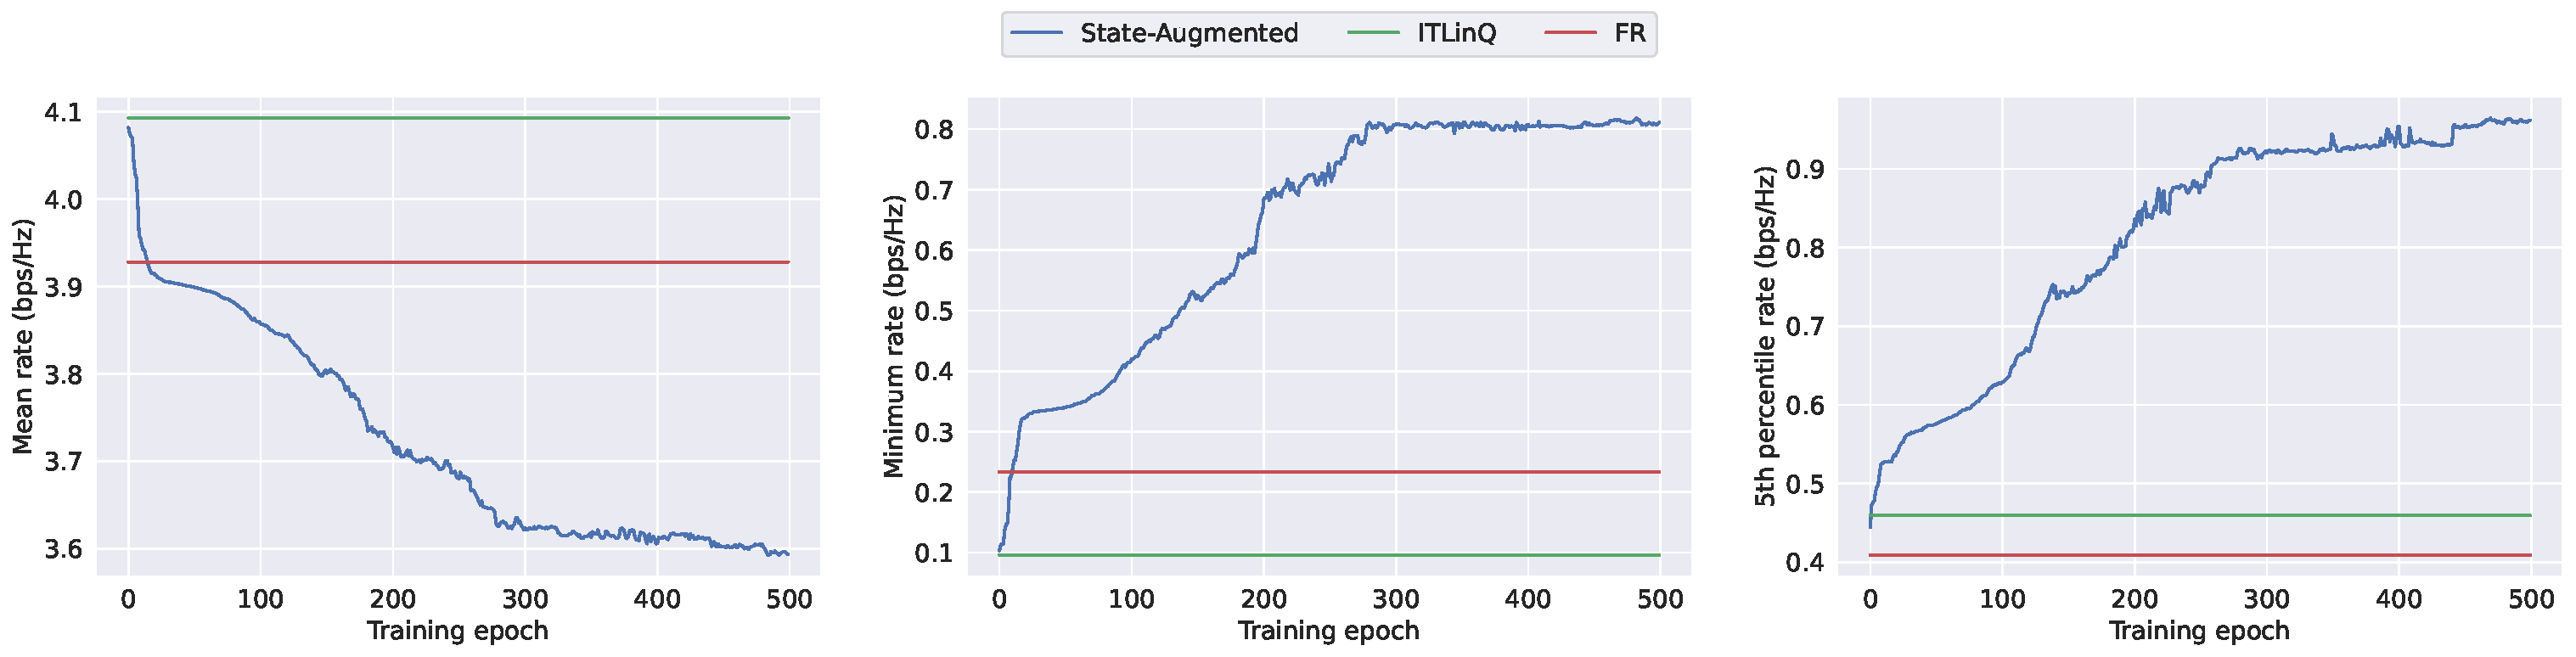
\includegraphics[width=\textwidth]{fig_convergence_singleConfig_m50_vardensity.pdf}
\caption{Convergence behavior of the proposed state-augmented RRM algorithm, and its comparison with the baseline methods for a \emph{single} network realization with $m=50$ transmitter-receiver pairs (variable-density scenario). Note that the baseline algorithms fail to achieve the minimum-rate requirement of $f_{\min}=0.6$, while our proposed method is able to satisfy the constraints for all $50$ users.
}
\label{fig:convergence_singleConfig_m50_vardensity}
\end{figure*}


\begin{figure*}[h]
\centering
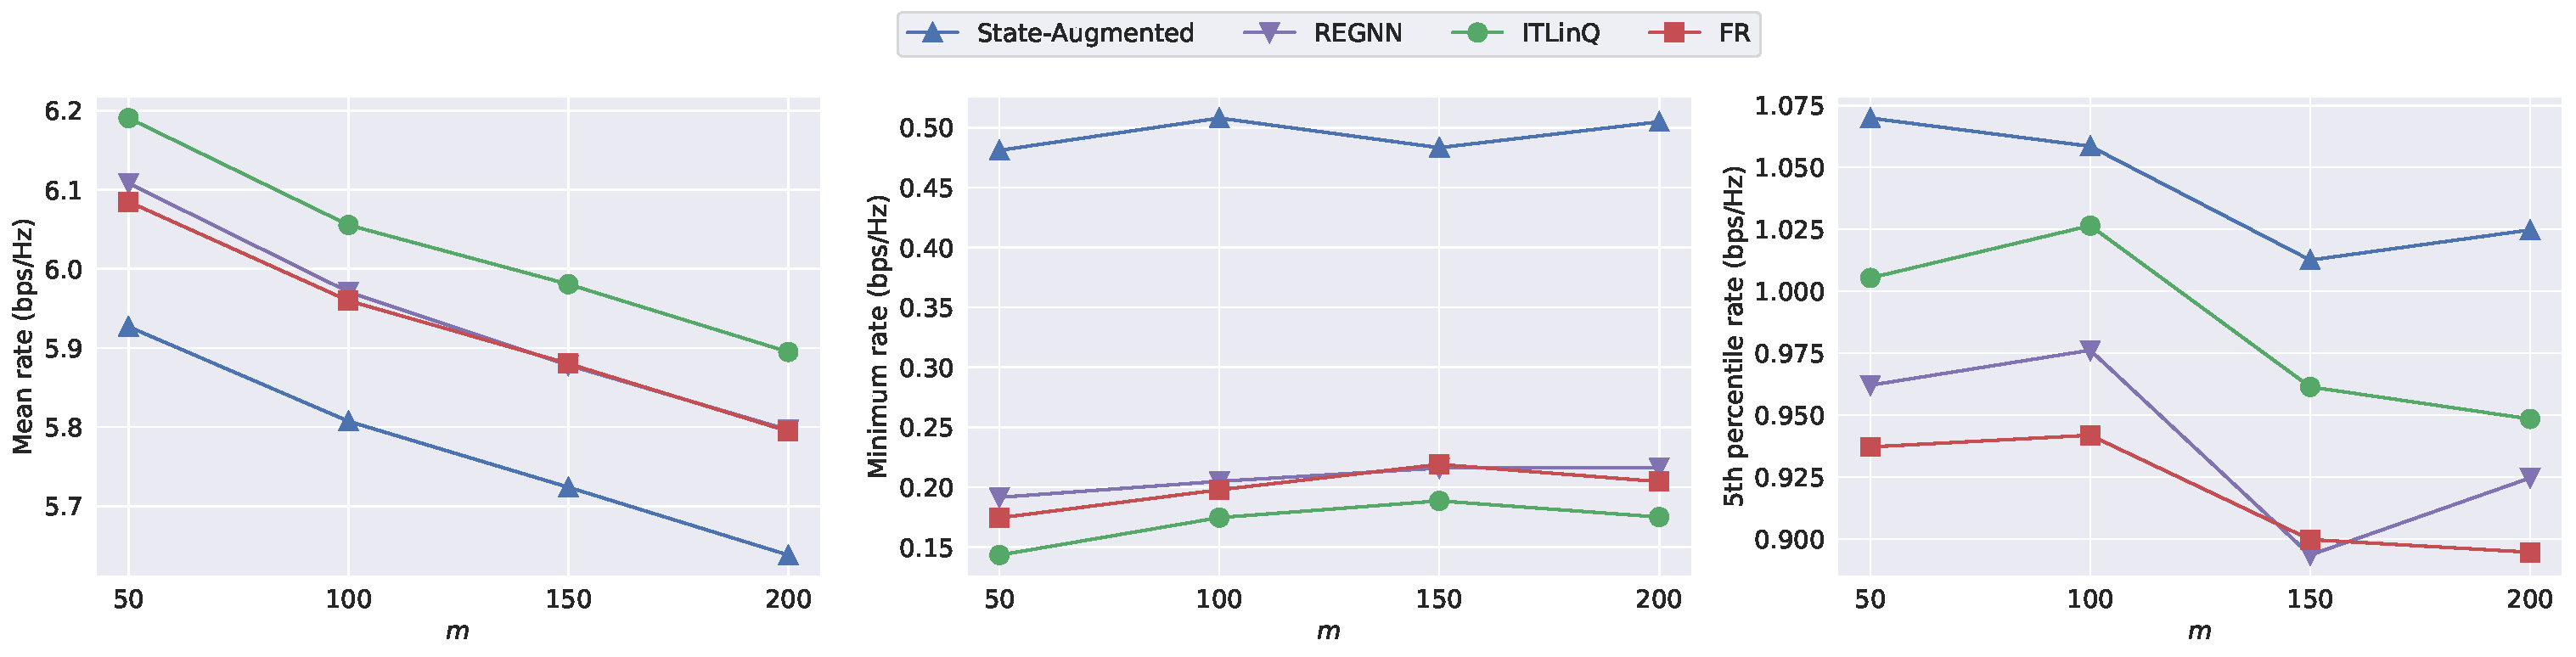
\includegraphics[width=\textwidth]{fig_scalability_fixed_density.pdf}
\caption{Performance comparison of the proposed state-augmented RRM algorithm against baseline methods in the fixed-density scenario for networks with $m\in\{50,100,150,200\}$ transmitter-receiver pairs.}
\label{fig:scalability_fixed_density}
\end{figure*}

\subsection{Experimental Results}\label{sec:exp_results}
We generate networks with $m$ transmitter-receiver pairs, located randomly within a square network area of side length $R$. We drop the transmitters uniformly at random within the network area, while ensuring a minimum distance of $75$m between each pair of them. Afterwards, for each transmitter, we drop its associated receiver uniformly at random within an annulus around the transmitter, with inner and outer radii of $10$m and $50$m, respectively. To control the network density, we consider the following two scenarios to determine the network area size:
\begin{itemize}
    \item \textbf{Fixed Density:} We set $R = \sqrt{m / 20} \times 2$km to keep the density constant (at $5$ users/km$^2$).
    \item \textbf{Variable Density:} We set $R=2$km, implying that the network density increases with $m$.
\end{itemize}
In both cases, and for all values of $m$, we set $f_{\min} = 0.6$bps/Hz, $T_0=5$, and $T=100$. We consider both large-scale and small-scale fading for the channel model. The large-scale fading follows a dual-slope path-loss model similar to~\cite{zhang2015downlink,andrews2016we,naderializadeh2022learning} alongside a $7$dB log-normal shadowing. Moreover, the small-scale fading models channel variations across different time steps following a Rayleigh distribution with a pedestrian speed of $1$m/s~\cite{li2002simulation}. We set the maximum transmit power to $P_{\max}=10$dBm, and the noise variance to $N=-104$dBm (due to the $10$MHz bandwidth and noise power spectral density of $-174$dBm/Hz).

We use a $3$-layer GNN with $F_1=F_2=64$, where the first two layers are based on the local extremum operator proposed in~\cite{ranjan2020asap}, while the last layer entails a linear projection (together with the mapping in~\eqref{eq:final_power_levels_GNN}). We set the primal and dual learning rates to $\eta_{\bbphi} = 10^{-1} / m$ and $\eta_{\bbmu} = 20$, respectively, and we set the batch size to $B=128$. For each value of $m$, we generate a total of $256$ training samples and $128$ samples for evaluation, where each sample refers to a realization of the transmitter/receiver locations (and the large-scale fading), alongside the small-scale fading random process. We set the normalization factor for edge weights at time step $t$ to $Z_t = \left\|\log\left(P_{\max}|\bbH_t|^2 / N\right)\right\|_2$. Except for the case of Section~\ref{sec:single_network} below, we run training for $100$ epochs, and we draw the dual variables during training randomly from the $U(0,1)$ distribution.

\urlstyle{tt}
As baselines, we compare the performance of our proposed method against three baselines: i) Full reuse (FR), where every transmitter uses $P_{\max}$; ii) Information-theoretic link scheduling (ITLinQ)~\cite{naderializadeh2014itlinq}, and iii) random-edge graph neural networks (REGNN)~\cite{eisen2020optimal}.\footnote{For a fair comparison with~\cite{eisen2020optimal}, we use the same exact GNN structure and hyperparameters as for our method to implement the REGNN method.} We would like to point out that, while the REGNN baseline allows the consideration of minimum-rate constraints, the first two baselines (i.e., FR and ITLinQ) are not able to handle such per-user requirements. In what follows, we primarily report the results in terms of three separate metrics, namely the mean rate, minimum rate (discarding the bottom 1\% of user rates as outliers), and the 5\textsuperscript{th} percentile rate, evaluated over the test configurations.\footnote{Our code is available at \url{https://github.com/navid-naderi/StateAugmented_RRM_GNN}.}




\begin{figure*}[h]
\centering
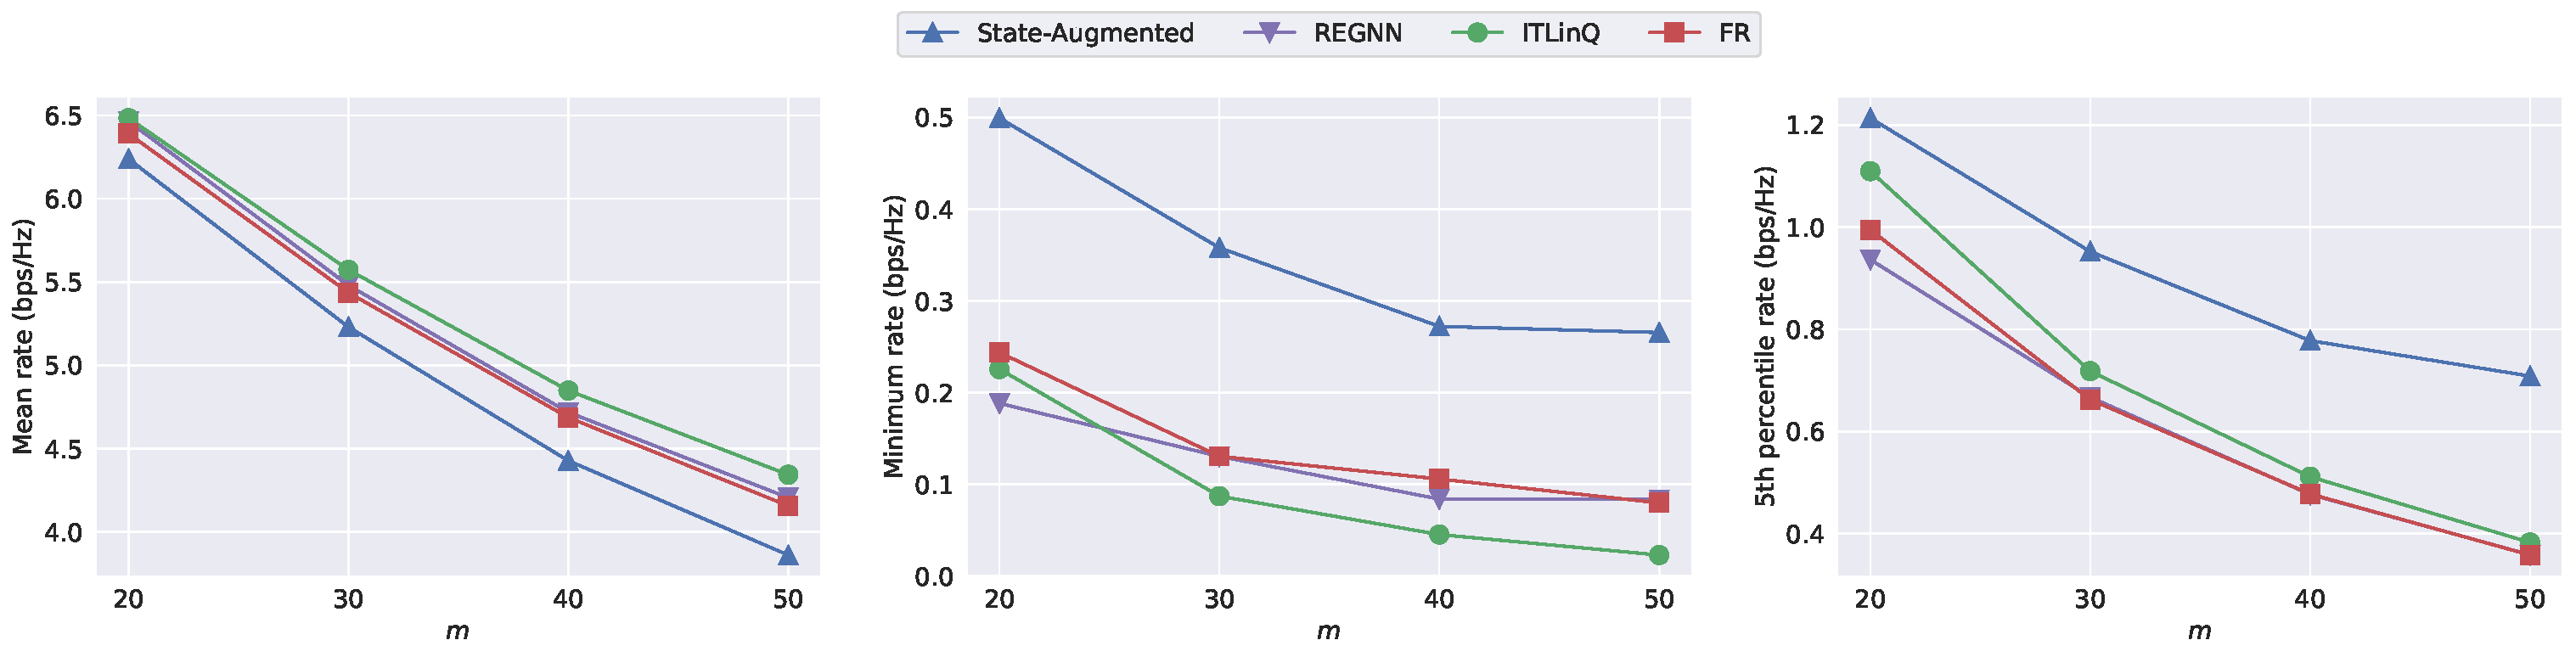
\includegraphics[width=\textwidth]{fig_scalability_variable_density.pdf}
\caption{Performance comparison of the proposed state-augmented RRM algorithm against baseline methods in the variable-density scenario for networks with $m\in\{20, 30, 40, 50\}$ transmitter-receiver pairs.}
\label{fig:scalability_variable_density}
\end{figure*}


\begin{figure*}[t!]
    \centering
    \begin{subfigure}[t]{0.5\textwidth}
        \centering
        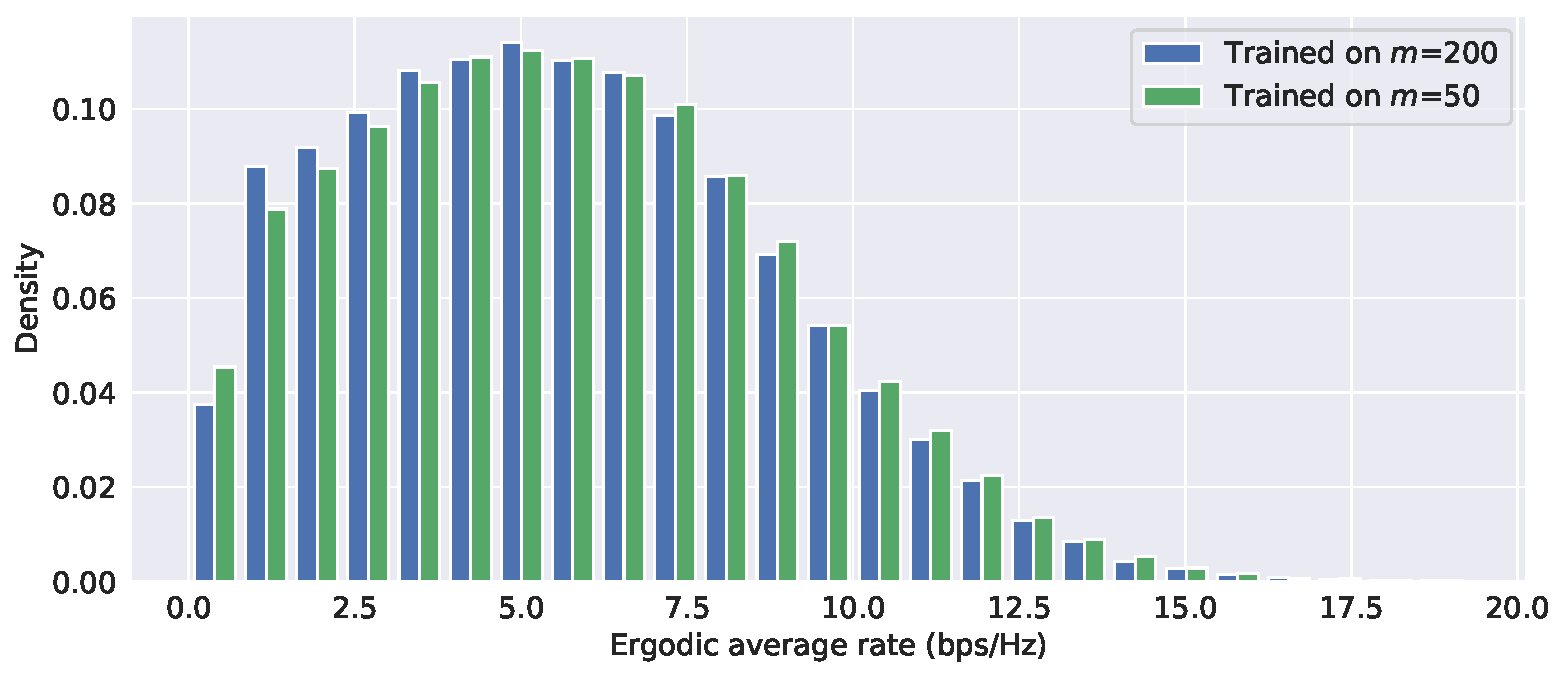
\includegraphics[width=.95\textwidth]{fig_transfer_fixed_density_50To200.pdf}
        \caption{\hspace*{-.25in}}
        \label{fig:transfer_fixed_density_50To200}
    \end{subfigure}%
    \hfill
    \begin{subfigure}[t]{0.5\textwidth}
        \centering
        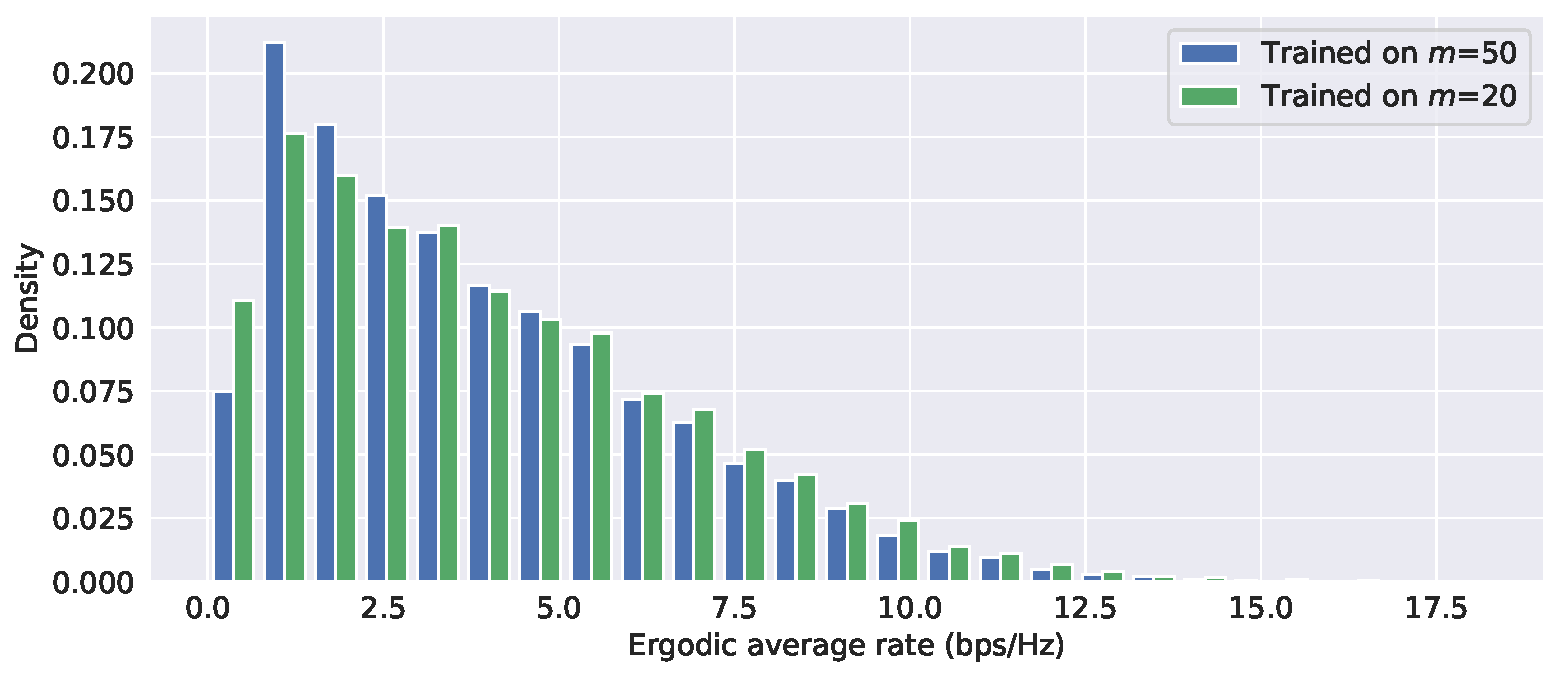
\includegraphics[width=.95\textwidth]{fig_transfer_variable_density_20To50.pdf}
        \caption{\hspace*{-.25in}}
        \label{fig:transfer_variable_density_20To50}
    \end{subfigure}%
    \caption{Transferability of the proposed state-augmented RRM procedure, shown as the histogram of ergodic average rates, for the (a) fixed-density scenario, evaluated on samples with $m=200$, and (b) variable-density scenario, evaluated on samples with $m=50$.}
    \label{fig:transferability}
\end{figure*}

\begin{figure*}[h]
\centering
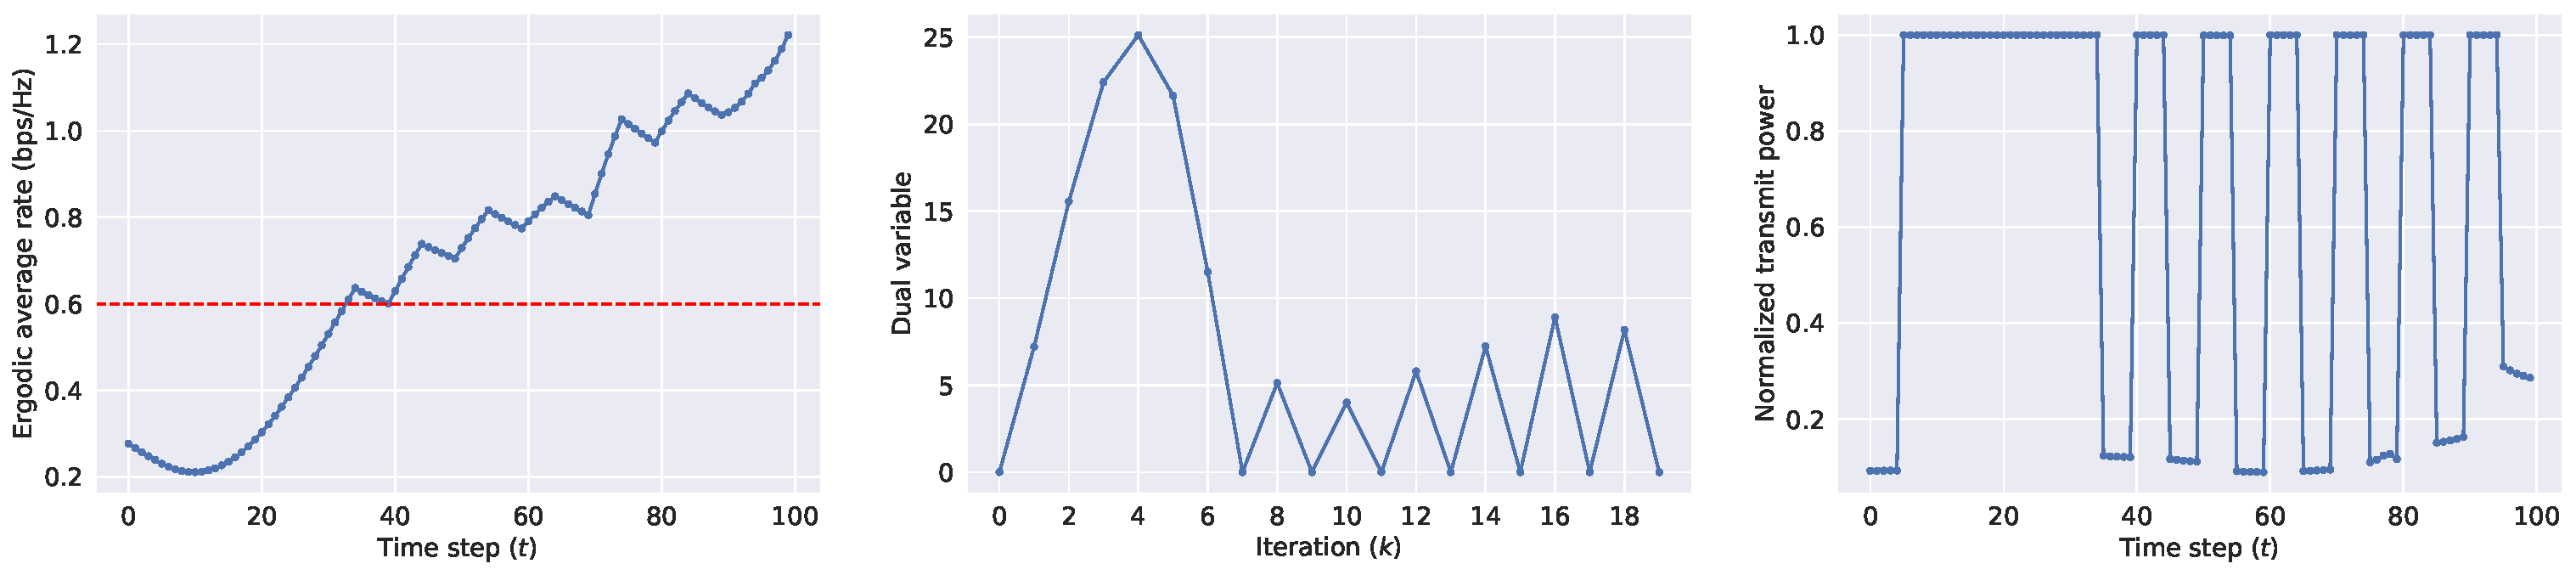
\includegraphics[width=\textwidth]{fig_policy_switching_m50_vardensity.pdf}
\caption{Evolution of the ergodic average rate (left), dual variable (middle), and normalized transmit power level (right) for an example user in a network with $m=50$ transmitter-receiver pairs (for the variable-density scenario). The dashed line in the left plot represents the minimum-rate requirement, i.e., $f_{\min}=0.6$.}
\label{fig:policy_switching_m50_vardensity}
\end{figure*}

\begin{figure}[h]
\centering
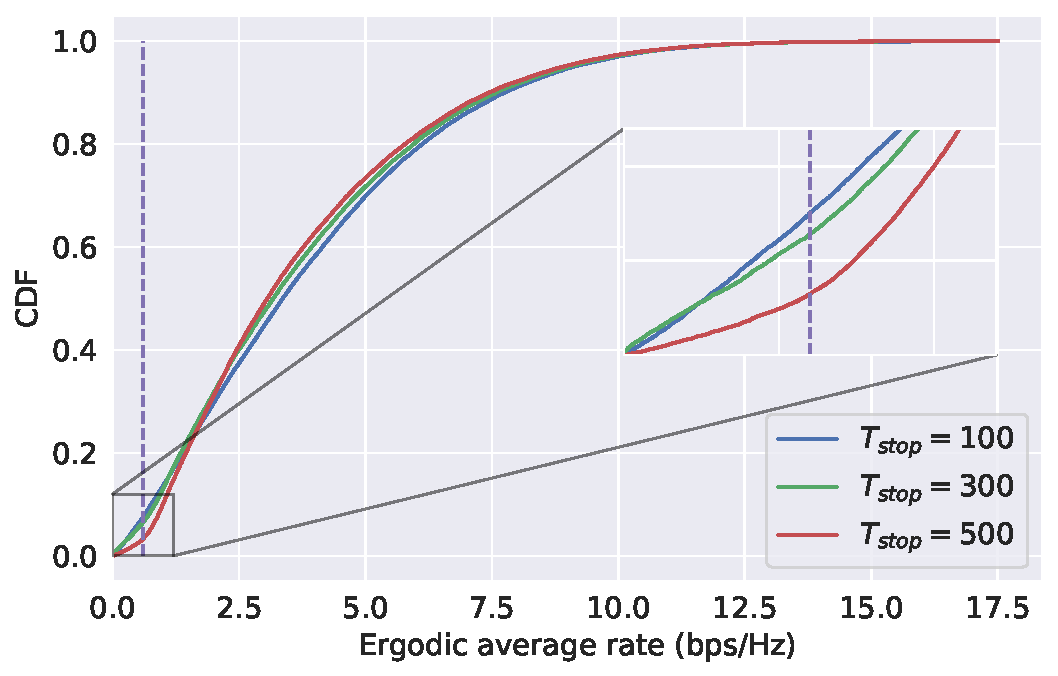
\includegraphics[width=.95\columnwidth]{fig_early_stopping_m50_vardensity_T500.pdf}
\caption{Impact of the early stopping of the dual descent updates on users' ergodic average rates in networks with $m=50$ transmitter-receiver pairs (for the variable-density scenario). The dashed line represents the minimum-rate requirement, i.e., $f_{\min}=0.6$.}
\label{fig:early_stopping_m50_vardensity_T500}
\end{figure}

% \begin{figure*}[h]
% \centering
% \includegraphics[width=\textwidth]{figs/impactoffmin_m6_T0_5.pdf}
% \caption{Impact of the minimum-rate constraint lower bound, $f_{\min}$, on the performance achieved by the proposed state-augmented RRM algorithm in networks with $m=6$ transmitter-receiver pairs (for the variable-density scenario).}
% \label{fig:impactoffmin_m6_T0_5}
% \end{figure*}


\subsubsection{Single Network Realization}\label{sec:single_network}
Figure~\ref{fig:convergence_singleConfig_m50_vardensity} shows the performance of our proposed method against the baselines for a \emph{single} network realization with $m=50$ users (in the variable-density scenario). For this specific experiment, we continue training for $500$ epochs, and decay the primal learning rate by $0.5$ every $100$ epochs. At the end of each training epoch, we evaluate the RRM algorithm on the same realization that is used for training. As the figure shows, our proposed state-augmented RRM algorithm considerably gains over the baseline algorithms in terms of the minimum and 5\textsuperscript{th} percentile rates, managing to satisfy the minimum-rate requirements for all users at the expense of a smaller achieved mean rate.

\subsubsection{Scalability}
Here, we assess the performance of the the proposed algorithm in \emph{families} of networks with different numbers of users, where the policies trained on samples with a specific value of $m$ are evaluated on test samples with the same value of $m$. Figures~\ref{fig:scalability_fixed_density} and~\ref{fig:scalability_variable_density} compare the performance of our proposed method with the baseline algorithms in the fixed-density and variable-density scenarios, respectively. In both scenarios, thanks to the feasibility guarantees of our proposed method for the per-user minimum-rate constraints, our method significantly outperforms the baseline methods in terms of the minimum rate and the 5\textsuperscript{th} percentile rate. This, however, comes at the cost of a slightly lower mean rate. Note that such a scalability is due to the size-invariant property of GNN-based parameterizations (where the number of parameters is fixed regardless of the graph size), as opposed to other parameterizations, such as multi-layer perceptrons (i.e., fully-connected neural networks).

\subsubsection{Transferability to Unseen Network Sizes}
Another upside of the size-invariance property of GNNs is that they can be evaluated on graph sizes not encountered throughout the training process. Figure~\ref{fig:transfer_fixed_density_50To200} shows the histogram of user ergodic average rates under our proposed algorithm in test networks of size $m=200$ (fixed-density scenario) using two GNNs: one trained on samples with $m=200$ and the other trained on samples with $m=50$. Moreover, Figure~\ref{fig:transfer_variable_density_20To50} shows a similar histogram for the variable-density scenario, where GNNs trained on samples with $m=50$ and $m=20$ are evaluated on test samples with $m=50$. As the figures show, in both cases, the trained GNNs provide excellent transferability to larger network sizes, achieving user rates that are similar to the GNNs without the train/test mismatch. Moreover, as expected, the transferred performance is more desirable in the fixed-density scenario than the variable-density scenario, as the channel statistics mostly remain similar in the former case, while in the latter case, the network becomes more interference-limited as $m$ grows.


\subsubsection{Policy Switching}
Figure~\ref{fig:policy_switching_m50_vardensity} shows what an example receiver experiences over the course of the $T=100$ time steps in a test network with $m=50$ transmitter-receiver pairs (for the variable-density scenario) once training is completed. Letting $i$ denote the receiver index, at each time step $t$, we plot its ergodic average rate up to that time step (i.e., $\frac{1}{t} \sum_{\tau=1}^t f_i(\bbH_{\tau}, \bbp(\bbH_{\tau},\bbmu_{\lfloor \tau / T_0 \rfloor};\bbphi^{\star}))$), its dual variable at the corresponding iteration (i.e., $\mu_{i,\lfloor t / T_0 \rfloor}$), and the selected normalized transmit power of transmitter $i$ at that time step (i.e., $p_i(\bbH_t,\bbmu_{\lfloor t / T_0 \rfloor};\bbphi^{\star}) / P_{\max}$). As the figure shows, a \emph{policy switching} behavior occurs, where for the time steps in which the receiver's ergodic average rate is below $f_{\min}$, the dual variable increases, leading to the corresponding transmitter using full transmit power. Moreover, when the ergodic average rate exceeds $f_{\min}$, the transmitter uses an on-off pattern to maintain its receiver's high ergodic average rate, while minimizing the interference caused at other receivers. This shows why state-augmentation is crucial for the algorithm to be able to switch the policy if/when necessary, depending on the constraint violations over time. Indeed, neither the ``off'' policy ($p_i=0$) nor the ``on'' policy ($p_i=P_{\max}$) guarantees the satisfaction of the constraints by itself. However, the illustrated policy switching behavior in Figure~\ref{fig:policy_switching_m50_vardensity} is exactly what the transmitters need to show in order to be able to satisfy their constraints in the long run.

\subsubsection{Drawback of Early Stopping of Dual Descent Iterations}
As we mentioned in Section~\ref{sec:alg}, the feasibility and near-optimality of the RRM decisions depend on the fact that the dual descent iterations in~\eqref{eq:mu_dynamics_augmented} continue for the entire duration of the execution phase. This implies that such feasibility and near-optimality guarantees will not hold if the dual descent updates are stopped at a small, finite number of iterations. Figure~\ref{fig:early_stopping_m50_vardensity_T500} illustrates the empirical cumulative distribution function (CDF) of the user ergodic average rates in test networks with $m=50$ transmitter-receiver pairs (for the variable-density scenario), where the dual descent updates are stopped at a certain time step $T_{\text{stop}} \in \{100, 300, 500\}$. For the sake of this experiment, we expanded the execution time horizon to $T=500$ time steps. As the figure shows, early stopping of the dual variable updates leads to a larger fraction of users violating their minimum-rate requirements. Quite interestingly, such an early stopping provides an equivalent way of implementing the regular primal-dual REGNN method in~\cite{eisen2020optimal}.

\subsubsection{Inference Computational Complexity}
The size-invariance property of the GNNs implies that the number of GNN parameters does not depend on the underlying graph size on which the GNN is operating. However, using GNNs on larger graph sizes naturally leads to a higher computational complexity. Figure~\ref{fig:inference_time_vs_m} shows the average inference time (on CPU) for graphs corresponding to networks with $m\in[20, 200]$ transmitter-receiver pairs. Note that, in practice, the inference time can effectively be reduced by parallelizing computations on GPU hardware architectures.

\begin{figure}[t!]
\centering
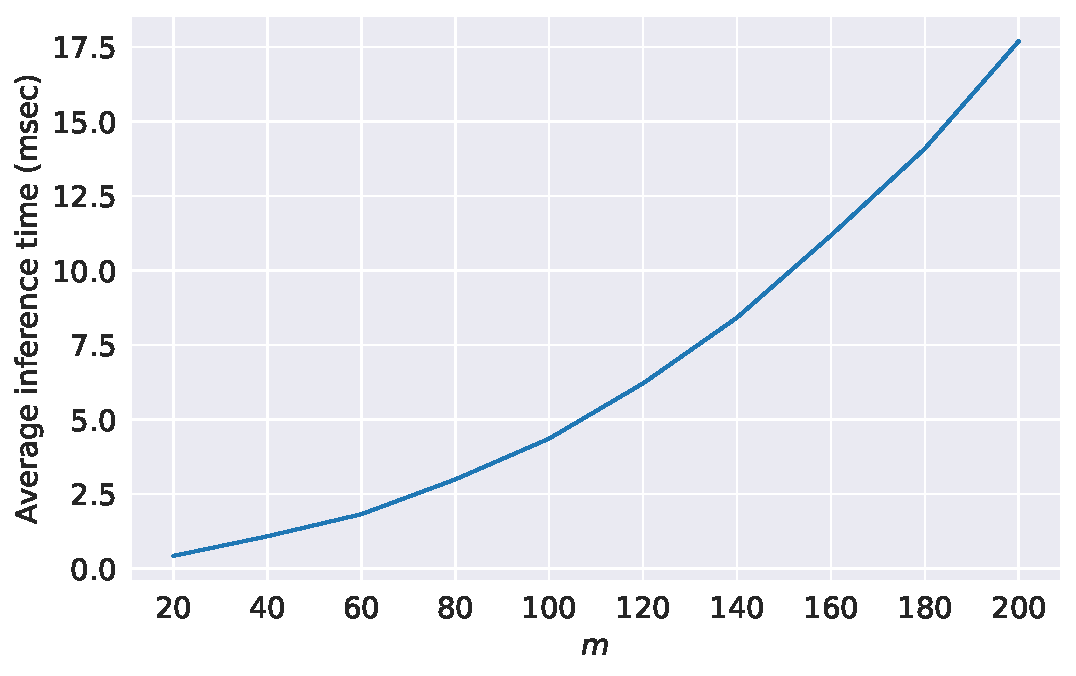
\includegraphics[width=.97\columnwidth]{fig_inference_time_vs_m.pdf}
\caption{Average inference time (on a CPU hardware architecture) for networks with $m\in[20,200]$ transmitter-receiver pairs.}
\label{fig:inference_time_vs_m}
\end{figure}


% \subsubsection{Impact of the Minimum-Rate Constraint Lower Bounds}
% In all our experiments, we set the lower bounds for the minimum-rate constraints, i.e., $f_{\min}$ to $\frac{3}{4}$. This resulted in RRM decisions that attempted to satisfy relatively strict minimum-rate constraints for almost all network realizations, which came at the cost of lower mean rates as compared to baseline methods. Figure~\ref{fig:impactoffmin_m6_T0_5} demonstrates the impact of the constraint lower bounds $f_{\min} \in \left\{\frac{1}{4}, \frac{1}{2}, \frac{3}{4}, 1\right\}$ on the performance of the proposed state-augmented RRM algorithm when trained and evaluated on networks with $m=6$ transmitter-receiver pairs (in the variable-density scenario). As the figure shows, tuning $f_{\min}$ reveals the trade-off between the average and worst-case performance of users across all network realizations. Finding the best minimum-rate constraint lower bound is a non-trivial problem, and it has also been shown that this bound can be tuned adaptively based on each specific network realization through the introduction of learnable slack parameters~\cite{naderializadeh2020wireless, naderializadeh2022learning, naderializadeh2022adaptive}. We leave the incorporation of adaptive minimum-rate constraints into state-augmented RRM algorithms as future work.

\section{Concluding Remarks}\label{sec:conclusion}
We considered the problem of resource allocation in wireless network, termed radio resource management (RRM), in which the goal is to maximize a network-wide utility subject to constraints on the long-term average performance of the network users. We showed how parameterized dual-based RRM policies can lead to feasible and near-optimal solutions, but suffer from multiple challenges, including that they need to be run for an infinite number of time steps and the model parameters have to be optimized for any given set of dual variables at every time step. To mitigate these challenges, we proposed a state-augmented RRM algorithm, which revises the parameterization to take as input the network state, as well as the dual variable at each step, and produce as output the RRM decisions. We showed that for near-universal parameterizations, the proposed method also leads to feasible and near-optimal sequences of RRM decisions. Using graph neural network (GNN) architectures to parameterize the state-augmented RRM policy, we also demonstrated, via a set of numerical experiments, that the proposed method provides scalable and transferable wireless power control solutions that outperform baseline algorithms.




\appendices
\section{Proof of Theorem~\ref{thm:main}}\label{appx:proof}
\allowdisplaybreaks

The arguments used in the proof of Theorem~\ref{thm:main} follow similar steps to those in~\cite{calvo2021state}, with some minor differences specific to our problem formulation, as outlined in Remark~\ref{remark:proof_diff}. We, therefore, include the complete proof here for the paper to be self-complete.% there are differences with prior proofs, specific to our problem formulation, that require us to include the complete proof here.

\subsection{Tightness of The Sequence of Dual Variable Probability Measures}\label{appx:proof_tightness}
We start by proving that the sequence of dual variable probability measures, i.e., $\{p(\bbmu_k|\bbmu_0)\}_{k}$, is tight in the following lemma.

\begin{lemma}
For any $\delta > 0$, there exists a compact set $\ccalA_{\delta}$ such that for every $k \geq 0$, we have $\mathsf{Pr}[\bbmu_k \in \ccalA_{\delta}] > 1 - \delta$.
\end{lemma}

\begin{proof}
Define the dual function, $d(\bbmu)$ as
\begin{align}\label{eq:def_dual_function}
d(\bbmu) = \max_{\bbtheta\in\bbTheta} \ccalL(\bbtheta, \bbmu),
\end{align}
and consider the following set:
\begin{align}\label{eq:def_C}
\ccalC = \left\{\bbmu \in \reals_+^c : d(\bbmu) - P^{\star} \leq \frac{c\eta_{\bbmu}G^2}{2} \right\}.
\end{align}
Now, let
\begin{align}
\ccalA_{\delta} = \ccalB_{\delta} \cup \left(\ccalC \oplus \ccalS_{\sqrt{c\eta_{\bbmu}^2 G^2}}\right),
\end{align}
where $\oplus$ denotes Minkowski sum, $\ccalS_r$ denotes a ball centered at the origin with radius $r\geq0$, and $\ccalB_{\delta}$ is defined as
\begin{align}
\ccalB_{\delta} = \left\{\bbmu \in \reals_+^c : \frac{\| \bbmu - \bbmu^{\star} \|}{\| \bbmu_0 - \bbmu^{\star}\|} \leq \frac{1}{\delta} \right\},
\end{align}
with $\bbmu^{\star}$ representing the optimal set of dual variables. Then, we have
\begin{align}
&\mathsf{Pr}[\bbmu_k \in \ccalA_{\delta}] \nonumber \\
& = \mathsf{Pr}\left[\bbmu_k \in \ccalB_{\delta} \cup \left(\ccalC \oplus \ccalS_{\sqrt{c\eta_{\bbmu}^2 G^2}}\right) \right] \\
& = \underbrace{\mathsf{Pr}\left[\bbmu_k \in \ccalB_{\delta} \cup \left(\ccalC \oplus \ccalS_{\sqrt{c\eta_{\bbmu}^2 G^2}}\right) \middle| \bbmu_{k-1}\in\ccalC \right]}_{\overset{(a)}{=}1} \cdot \ p \nonumber \\
& \quad + \underbrace{\mathsf{Pr}\left[\bbmu_k \in \ccalB_{\delta} \cup \left(\ccalC \oplus \ccalS_{\sqrt{c\eta_{\bbmu}^2 G^2}}\right) \middle| \bbmu_{k-1}\in\ccalC^c \right]}_{\geq \mathsf{Pr}\left[\bbmu_k \in \ccalB_{\delta}  \middle| \bbmu_{k-1}\in\ccalC^c \right]} \cdot \ (1-p) \nonumber \\
& \geq \mathsf{Pr}\left[\bbmu_k \in \ccalB_{\delta}  \middle| \bbmu_{k-1}\in\ccalC^c \right] \\
& = \mathsf{Pr}\left[\frac{\| \bbmu_k - \bbmu^{\star} \|}{\| \bbmu_0 - \bbmu^{\star}\|} \leq \frac{1}{\delta}  \middle| \bbmu_{k-1}\in\ccalC^c \right] \\
& \geq 1 - \left( \frac{\E\left[\| \bbmu_k - \bbmu^{\star} \| \middle| \bbmu_{k-1}\in\ccalC^c\right]}{\| \bbmu_0 - \bbmu^{\star}\|} \right) \delta,
\end{align}
where $p=\mathsf{Pr}\left[\bbmu_{k-1}\in\ccalC \right]$, (a) is true due to the dual dynamics in~\eqref{eq:mu_dynamics} and the fact that the change between $\bbmu_{k-1}$ and $\bbmu_k$ is upper bounded in norm by $\sqrt{c\eta_{\bbmu}^2 G^2}$, and the last inequality is due to conditional Markov's inequality. Therefore, to complete the proof, it suffices to show that (i)
\begin{align}\label{eq:bounded_conditional_difference_norm_muk}
\E\left[\| \bbmu_k - \bbmu^{\star} \| \middle| \bbmu_{k-1}\in\ccalC^c\right] < \| \bbmu_0 - \bbmu^{\star}\|,
\end{align}
and (ii) that $\ccalA_{\delta}$ is compact.

\noindent\textbf{Proof of~\eqref{eq:bounded_conditional_difference_norm_muk}.}
Let $\Delta_{\bbmu_{k-1}}$ be defined as
\begin{align}
\Delta_{\bbmu_{k-1}} \coloneqq \bbg\left( \frac{1}{T_0} \sum_{t=(k-1)T_0}^{kT_0-1} \bbf(\bbH_{t}, \bbp(\bbH_{t};\bbtheta_{k-1})) \right).
\end{align}
Then, from the dual dynamics in~\eqref{eq:mu_dynamics}, we have
\begin{align*}
&\|\bbmu_{k} - \bbmu^{\star}\|^2 \\
&\leq \|\bbmu_{k-1} - \bbmu^{\star} - \eta_{\bbmu} \Delta_{\bbmu_{k-1}} \|^2 \\
&= \|\bbmu_{k-1} - \bbmu^{\star}  \|^2 + \eta_{\bbmu}^2 \|\Delta_{\bbmu_{k-1}} \|^2 \nonumber \\
&\quad - 2\eta_{\bbmu} (\bbmu_{k-1} - \bbmu^{\star})^T \Delta_{\bbmu_{k-1}} \\
&\leq \|\bbmu_{k-1} - \bbmu^{\star}  \|^2 + c \eta_{\bbmu}^2 G^2 - 2\eta_{\bbmu} (\bbmu_{k-1} - \bbmu^{\star})^T \Delta_{\bbmu_{k-1}},
\end{align*}
where the last inequality follows from the fact that for any $i\in\{1,\dots,c\}$, we assume $|g_i\left(\cdot\right)|\leq G$. Taking the expectation of both sides conditioned on $\bbmu_{k-1}$, we have
\begin{align}
&\E\left[\|\bbmu_{k} - \bbmu^{\star}\|^2 \middle| \bbmu_{k-1}\right] \nonumber\\
&\leq \|\bbmu_{k-1} - \bbmu^{\star}  \|^2 + c \eta_{\bbmu}^2 G^2 \nonumber \\
&\quad - 2\eta_{\bbmu} (\bbmu_{k-1} - \bbmu^{\star})^T \E\left[\Delta_{\bbmu_{k-1}}\middle| \bbmu_{k-1}\right]\\
&\leq \|\bbmu_{k-1} - \bbmu^{\star}  \|^2 + c \eta_{\bbmu}^2 G^2 - 2\eta_{\bbmu} (d(\bbmu_{k-1}) - d(\bbmu^{\star}))\label{eq:subgradient}\\
&= \|\bbmu_{k-1} - \bbmu^{\star}  \|^2 + c \eta_{\bbmu}^2 G^2 - 2\eta_{\bbmu} (d(\bbmu_{k-1}) - P^{\star}),\label{eq:pre_C_bound}
\end{align}
where~\eqref{eq:subgradient} follows from the fact that $\Delta_{\bbmu_{k-1}}$ is a subgradient of the dual function~\cite{danskin2012theory}, leading to the inequality $(\bbmu_{k-1} - \bbmu^{\star})^T \E\left[\Delta_{\bbmu_{k-1}}\middle| \bbmu_{k-1}\right] \geq d(\bbmu_{k-1}) - d(\bbmu^{\star})$ thanks to the dual function being convex~\cite{boyd2004convex}. Now, combining the fact that $\bbmu_{k-1}\in\ccalC^c$ with the definition of $\ccalC$ in~\eqref{eq:def_C}, we can continue~\eqref{eq:pre_C_bound} as
\begin{align}
\E\left[\|\bbmu_{k} - \bbmu^{\star}\|^2 \middle| \bbmu_{k-1}\in\ccalC^c\right]
&< \|\bbmu_{k-1} - \bbmu^{\star}\|^2 \\
&< \|\bbmu_{0} - \bbmu^{\star}\|^2,
\end{align}
with the last inequality following from recursion.


\noindent\textbf{Proof of Compactness of $\ccalA_{\delta}$.} Since the Minkowski sum of two compact sets is compact, and also the union of two compact sets is compact, it suffices to show that the set $\ccalC$ is compact.

Given the definition of the dual function in~\eqref{eq:def_dual_function}, for any set of model parameters $\bbtheta\in\bbTheta$ and any set of dual variables $\bbmu\in\reals_+^c$, we have
\begin{align}
d(\bbmu) &\geq \mathcal{U}\left( \frac{1}{T} \sum_{t=0}^{T-1} \bbf(\bbH_t, \bbp(\bbH_t;\bbtheta)) \right)\nonumber \\
   &\qquad\qquad+ \bbmu^T \bbg\left( \frac{1}{T} \sum_{t=0}^{T-1} \bbf(\bbH_t, \bbp(\bbH_t;\bbtheta)) \right)
\end{align}
Now, replacing $\bbtheta$ with the strictly-feasible set of model parameters $\hat{\bbtheta}$ considered in Theorem~\ref{thm:main}, we can write
\begin{align}
d(\bbmu) &\geq \mathcal{U}\left( \frac{1}{T} \sum_{t=0}^{T-1} \bbf(\bbH_t, \bbp(\bbH_t;\hat{\bbtheta})) \right)\nonumber \\
   &\qquad\qquad+ \bbmu^T \bbg\left( \frac{1}{T} \sum_{t=0}^{T-1} \bbf(\bbH_t, \bbp(\bbH_t;\hat{\bbtheta})) \right)\\
&\geq \mathcal{U}\left( \frac{1}{T} \sum_{t=0}^{T-1} \bbf(\bbH_t, \bbp(\bbH_t;\hat{\bbtheta})) \right) + G' \| \bbmu \|_1.\label{eq:dual_upper_bound}
\end{align}
Now, for any $\bbmu\in\ccalC$, according to the definition in~\eqref{eq:def_C}, the bound in~\eqref{eq:dual_upper_bound} leads to
\begin{align}
P^{\star} + \frac{c\eta_{\bbmu}G^2}{2}  \geq \mathcal{U}\left( \frac{1}{T} \sum_{t=0}^{T-1} \bbf(\bbH_t, \bbp(\bbH_t;\hat{\bbtheta})) \right) + G' \| \bbmu \|_1,
\end{align}
implying that $\bbmu$ belongs to the following ball,
\begin{align}
\| \bbmu \|_1 \leq \frac{P^{\star} + \frac{c\eta_{\bbmu}G^2}{2} - \mathcal{U}\left( \frac{1}{T} \sum_{t=0}^{T-1} \bbf(\bbH_t, \bbp(\bbH_t;\hat{\bbtheta})) \right)}{G'},
\end{align}
hence completing the proof.


\end{proof}

\subsection{Proof of Feasibility in~\eqref{eq:thm_feasibility}}\label{appx:proof_feasibility}

From the dual dynamics in~\eqref{eq:mu_dynamics}, we have
\begin{align}\label{eq:mu_inequality}
% \bbmu_{T+1} &\geq \bbmu_T - \eta_{\bbmu} \bbg\left(  \bbf(\bbH_T, \bbp(\bbH_T;\bbtheta_T)) \right).
\bbmu_{K} &\geq \bbmu_{K-1} - \eta_{\bbmu} \bbg\left( \frac{1}{T_0} \sum_{t=(K-1)T_0}^{KT_0-1} \bbf(\bbH_{t}, \bbp(\bbH_{t};\bbtheta_{K-1})) \right)\hspace{-3pt}.
\end{align}
Using the inequality in~\eqref{eq:mu_inequality} recursively yields
% \begin{align}
% \bbmu_{T+1} &\geq \bbmu_1 - \eta_{\bbmu} \sum_{t=1}^T \bbg\left(  \bbf(\bbH_t, \bbp(\bbH_t;\bbtheta_t)) \right) \\
% &= \bbmu_1 - T \eta_{\bbmu} \left(\frac{1}{T} \sum_{t=1}^T  \bbg\left(  \bbf(\bbH_t, \bbp(\bbH_t;\bbtheta_t)) \right)\right) \\
% &\geq \bbmu_1 - T \eta_{\bbmu}  \bbg\left( \frac{1}{T} \sum_{t=1}^T  \bbf(\bbH_t, \bbp(\bbH_t;\bbtheta_t)) \right),
% \end{align}
\begin{align*}
&\bbmu_{K} \nonumber \\
&\geq \bbmu_0 - \eta_{\bbmu} \sum_{k=0}^{K-1} \bbg\left( \frac{1}{T_0} \sum_{t=kT_0}^{(k+1)T_0-1} \bbf(\bbH_{t}, \bbp(\bbH_{t};\bbtheta_k)) \right) \nonumber \\
&= \bbmu_0 - K\eta_{\bbmu} \cdot \frac{1}{K}\hspace{-3pt}\sum_{k=0}^{K-1} \bbg\left( \frac{1}{T_0} \sum_{t=kT_0}^{(k+1)T_0-1} \bbf(\bbH_{t}, \bbp(\bbH_{t};\bbtheta_k)) \right) \nonumber \\
&\geq \bbmu_0 - K\eta_{\bbmu} \bbg\left( \frac{1}{KT_0} \sum_{t=0}^{KT_0-1} \bbf(\bbH_t, \bbp(\bbH_t;\bbtheta_{\lfloor t/T_0 \rfloor})) \right),
\end{align*}
where the last inequality follows from the concavity of $\bbg(\cdot)$. Therefore, we have
% \begin{align}\label{eq:muT+1_vs_mu1}
% &\limsup_{T\to\infty}\bbmu_{T+1}  \nonumber\\ 
% &\geq \bbmu_1 - \eta_{\bbmu} \liminf_{T\to\infty} T \bbg\left( \frac{1}{T} \sum_{t=1}^T  \bbf(\bbH_t, \bbp(\bbH_t;\bbtheta_t)) \right).
% \end{align}
\begin{align}\label{eq:muT+1_vs_mu1}
&\limsup_{K\to\infty}\bbmu_{K+1}  \nonumber\\ 
&\geq \bbmu_0 - \eta_{\bbmu} \liminf_{K\to\infty} K \bbg\left( \frac{1}{T} \sum_{t=0}^{T-1} \bbf(\bbH_t, \bbp(\bbH_t;\bbtheta_{\lfloor t/T_0 \rfloor})) \right).
\end{align}
Now, assume by contradiction that one of the constraints in~\eqref{eq:thm_feasibility} is not satisfied. More precisely, assume there exists an index $i\in\{1,\dots,c\}$ and positive constants $\delta>0$ and $\beta\in(0,1)$ such that
\begin{align}\label{eq:contradiction_prob}
\mathsf{Pr}\left[\liminf_{T\to\infty} g_i\left( \frac{1}{T} \sum_{t=0}^{T-1} \bbf(\bbH_t, \bbp(\bbH_t;\bbtheta_{\lfloor t/T_0 \rfloor})) \right) \leq -\delta \right] = \beta.
\end{align}
This implies that with non-zero probability $\beta$, we would have
% \begin{align}
% &\limsup_{T\to\infty} \|\bbmu_{T+1}\|_1 \nonumber \\
% &\geq \limsup_{T\to\infty} \mu_{i,T+1}\label{eq:1_norm} \\
% &\geq \mu_{i,1} - \eta_{\bbmu} \liminf_{T\to\infty} T g_i\left( \frac{1}{T} \sum_{t=1}^T  \bbf(\bbH_t, \bbp(\bbH_t;\bbtheta_t)) \right)\label{eq:ith_bound} \\
% &\geq \mu_{i,1} + \eta_{\bbmu} \liminf_{T\to\infty} T \epsilon \label{eq:contradiction_prob_use} \\
% &= \infty,
% \end{align}
\begin{align}
&\limsup_{K\to\infty} \|\bbmu_{K}\|_1 \nonumber \\
&\geq \limsup_{K\to\infty} \mu_{i,K}\label{eq:1_norm} \\
&\geq \mu_{i,0} - \eta_{\bbmu} \liminf_{K\to\infty} K g_i\left( \frac{1}{T} \sum_{t=0}^{T-1} \bbf(\bbH_t, \bbp(\bbH_t;\bbtheta_{\lfloor t/T_0 \rfloor})) \right)\label{eq:ith_bound} \\
&\geq \mu_{i,0} + \eta_{\bbmu} \liminf_{K\to\infty} K \epsilon \label{eq:contradiction_prob_use} \\
&= \infty,
\end{align}
where~\eqref{eq:1_norm} follows from the definition of the $\ell_1$-norm% and the fact that $\mu_{i,T+1} \geq 0$
,~\eqref{eq:ith_bound} follows from the $i$\textsuperscript{th} inequality in~\eqref{eq:muT+1_vs_mu1}, and~\eqref{eq:contradiction_prob_use} follows from~\eqref{eq:contradiction_prob}. This contradicts the fact that the sequence of dual variable probabilities is tight, hence completing the proof.
\hfill$\square$


\subsection{Proof of Optimality in~\eqref{eq:thm_optimality}}


Given the dual dynamics in~\eqref{eq:mu_dynamics} and the fact that projection onto the non-negative orthant does not increase the $\ell_2$-norm, we have
\begin{align}
&\left\|\bbmu_{K+1}\right\|^2\nonumber\\
&\leq \left\|\bbmu_K - \eta_{\bbmu} \bbg\left( \frac{1}{T_0} \sum_{t=KT_0}^{(K+1)T_0-1} \bbf(\bbH_{t}, \bbp(\bbH_{t};\bbtheta_K)) \right) \right\|^2\label{eq:norm_dual_update}\\
&=\left\|\bbmu_K \right\|^2 + \eta_{\bbmu}^2 \left\| \bbg\left( \frac{1}{T_0} \sum_{t=KT_0}^{(K+1)T_0-1} \bbf(\bbH_{t}, \bbp(\bbH_{t};\bbtheta_K)) \right)\right\|^2 \nonumber \\
&~\quad- 2\eta_{\bbmu}\bbmu_K^T \bbg\left( \frac{1}{T_0} \sum_{t=KT_0}^{(K+1)T_0-1} \bbf(\bbH_{t}, \bbp(\bbH_{t};\bbtheta_K)) \right)\label{eq:norm_dual_square_expansion}\\
&\leq\left\|\bbmu_T\right\|^2 + c\eta_{\bbmu}^2 G^2  \nonumber \\
&~\quad - 2\eta_{\bbmu}\bbmu_K^T \bbg\left( \frac{1}{T_0} \sum_{t=KT_0}^{(K+1)T_0-1} \bbf(\bbH_{t}, \bbp(\bbH_{t};\bbtheta_K)) \right),\label{eq:g_bounded}
\end{align}
% Since $\left\|\bbmu_{T+1}\right\|^2 \geq 0$, expanding the squared norm on the right-hand side of~\eqref{eq:norm_dual_update} yields
% \begin{align}\label{eq:norm_dual_square_expansion}
% 0 &\leq \left\|\bbmu_T\right\|^2 + \eta_{\bbmu}^2 \left\| \bbg\left(  \bbf(\bbH_T, \bbp(\bbH_T, \bbmu_T;\bbtheta)) \right)\right\|^2 - 2\eta_{\bbmu}\bbmu_T^T \bbg\left(  \bbf(\bbH_T, \bbp(\bbH_T, \bbmu_T;\bbtheta)) \right) .
% \end{align}
%Since 
where the last inequality follows from the fact that for any $i\in\{1,\dots,c\}$, we assume $|g_i\left(\cdot\right)|\leq G$. Applying~\eqref{eq:g_bounded} recursively yields
\begin{align}
&\left\|\bbmu_{K+1}\right\|^2 \nonumber\\
&\leq \left\|\bbmu_0\right\|^2 + c\eta_{\bbmu}^2 K G^2  \nonumber \\
&~\quad - 2\eta_{\bbmu} \sum_{k=0}^{K-1} \bbmu_k^T \bbg\left( \frac{1}{T_0} \sum_{t=kT_0}^{(k+1)T_0-1} \bbf(\bbH_{t}, \bbp(\bbH_{t};\bbtheta_k)) \right).\label{eq:g_bounded_recursive}
\end{align}
Since $\left\|\bbmu_{K+1}\right\|^2 \geq 0$, rearranging the terms in~\eqref{eq:g_bounded_recursive} and normalizing both sides by $2\eta_{\bbmu}K$ results in
% \begin{align}\label{eq:inner_prod_dual_init}
% \bbmu_T^T \bbg\left(  \bbf(\bbH_T, \bbp(\bbH_T, \bbmu_T;\bbtheta)) \right) \leq \frac{1}{2\eta_{\bbmu}}\left\|\bbmu_T\right\|^2 + \frac{c\eta_{\bbmu}G^2}{2}.
% \end{align}
% Applying~\eqref{eq:inner_prod_dual_init} recursively and normalizing by $T$, we will have
\begin{align}\label{eq:inner_prod_dual_recursive_normalized}
&\frac{1}{K} \sum_{k=0}^{K-1} \bbmu_k^T \bbg\left( \frac{1}{T_0} \sum_{t=kT_0}^{(k+1)T_0-1} \bbf(\bbH_{t}, \bbp(\bbH_{t};\bbtheta_k)) \right)\nonumber \\
&\leq \frac{1}{2\eta_{\bbmu}K} \left\|\bbmu_0\right\|^2 + \frac{c\eta_{\bbmu}G^2}{2}.
\end{align}
Taking the conditional expectation of both sides in~\eqref{eq:inner_prod_dual_recursive_normalized} given $\bbmu_0$, and letting $K\to\infty$, we can write
\begin{align}
&\limsup_{K\to\infty} \E\left[\sum_{k=0}^{K-1} \frac{\bbmu_k^T}{K} \bbg\left(  \sum_{t=kT_0}^{(k+1)T_0-1} \frac{\bbf(\bbH_{t}, \bbp(\bbH_{t};\bbtheta_k))}{T_0} \right)\middle|\bbmu_0\right] \nonumber \\
&\leq \frac{c\eta_{\bbmu}G^2}{2}.\label{eq:inner_prod_dual_limsup}
\end{align}


%%%% SINGLE-STEP MU UPDATES
% Given the dual dynamics in~\eqref{eq:mu_dynamics} and the fact that projection onto the non-negative orthant does not increase the $\ell_2$-norm, we have
% \begin{align}
% \left\|\bbmu_{T+1}\right\|^2 &\leq \left\|\bbmu_T - \eta_{\bbmu} \bbg\left(  \bbf(\bbH_T, \bbp(\bbH_T;\bbtheta_{\lfloor T / T_0 \rfloor})) \right)\right\|^2\label{eq:norm_dual_update}\\
% &=\left\|\bbmu_T\right\|^2 + \eta_{\bbmu}^2 \left\| \bbg\left(  \bbf(\bbH_T, \bbp(\bbH_T;\bbtheta_{\lfloor T / T_0 \rfloor})) \right)\right\|^2 \nonumber \\
% &~\quad- 2\eta_{\bbmu}\bbmu_T^T \bbg\left(  \bbf(\bbH_T, \bbp(\bbH_T;\bbtheta_{\lfloor T / T_0 \rfloor})) \right)\label{eq:norm_dual_square_expansion}\\
% &\leq\left\|\bbmu_T\right\|^2 + c\eta_{\bbmu}^2 G^2  \nonumber \\
% &~\quad - 2\eta_{\bbmu}\bbmu_T^T \bbg\left(  \bbf(\bbH_T, \bbp(\bbH_T;\bbtheta_{\lfloor T / T_0 \rfloor})) \right),\label{eq:g_bounded}
% \end{align}
% % Since $\left\|\bbmu_{T+1}\right\|^2 \geq 0$, expanding the squared norm on the right-hand side of~\eqref{eq:norm_dual_update} yields
% % \begin{align}\label{eq:norm_dual_square_expansion}
% % 0 &\leq \left\|\bbmu_T\right\|^2 + \eta_{\bbmu}^2 \left\| \bbg\left(  \bbf(\bbH_T, \bbp(\bbH_T, \bbmu_T;\bbtheta)) \right)\right\|^2 - 2\eta_{\bbmu}\bbmu_T^T \bbg\left(  \bbf(\bbH_T, \bbp(\bbH_T, \bbmu_T;\bbtheta)) \right) .
% % \end{align}
% %Since 
% where the last inequality follows from the fact that for any $k\in\{1,\dots,c\}$, we assume $|g_k\left(  \bbf(\bbH_T, \bbp(\bbH_T;\bbtheta_{\lfloor T / T_0 \rfloor}))\right)|\leq G$. Applying~\eqref{eq:g_bounded} recursively yields
% \begin{align}
% \left\|\bbmu_{T+1}\right\|^2 &\leq \left\|\bbmu_1\right\|^2 + c\eta_{\bbmu}^2 T G^2  \nonumber \\
% &~\quad - 2\eta_{\bbmu} \sum_{t=1}^T \bbmu_t^T \bbg\left(  \bbf(\bbH_t, \bbp(\bbH_t;\bbtheta_{\lfloor t / T_0 \rfloor})) \right).\label{eq:g_bounded_recursive}
% \end{align}
% Since $\left\|\bbmu_{T+1}\right\|^2 \geq 0$, rearranging the terms in~\eqref{eq:g_bounded_recursive} and normalizing both sides by $2\eta_{\bbmu}T$ results in
% % \begin{align}\label{eq:inner_prod_dual_init}
% % \bbmu_T^T \bbg\left(  \bbf(\bbH_T, \bbp(\bbH_T, \bbmu_T;\bbtheta)) \right) \leq \frac{1}{2\eta_{\bbmu}}\left\|\bbmu_T\right\|^2 + \frac{c\eta_{\bbmu}G^2}{2}.
% % \end{align}
% % Applying~\eqref{eq:inner_prod_dual_init} recursively and normalizing by $T$, we will have
% \begin{align}\label{eq:inner_prod_dual_recursive_normalized}
% \frac{1}{T} \sum_{t=1}^T \bbmu_t^T \bbg\left(  \bbf(\bbH_t, \bbp(\bbH_t;\bbtheta_{\lfloor t / T_0 \rfloor})) \right) \leq \frac{1}{2\eta_{\bbmu}T} \left\|\bbmu_1\right\|^2 + \frac{c\eta_{\bbmu}G^2}{2}.
% \end{align}
% Taking the conditional expectation of both sides in~\eqref{eq:inner_prod_dual_recursive_normalized} given $\bbmu_1$, and letting $T\to\infty$, we can write
% \begin{align}\label{eq:inner_prod_dual_limsup}
% \limsup_{T\to\infty}\frac{1}{T} \sum_{t=1}^T \E\left[\bbmu_t^T \bbg\left(  \bbf(\bbH_t, \bbp(\bbH_t;\bbtheta_{\lfloor t / T_0 \rfloor})) \right) | \bbmu_1 \right] \leq \frac{c\eta_{\bbmu}G^2}{2}.
% \end{align}



% {\color{black} %\textbf{Alternative solution:}

For any iteration $k$, since $\bbtheta_k$ is the maximizer of~\eqref{eq:theta_dynamics}, for any $\bbtheta\in\bbTheta$, we can write
\begin{align}
& \mathcal{U}\left( \frac{1}{T_0} \sum_{t=kT_0}^{(k+1)T_0-1} \bbf(\bbH_{t}, \bbp(\bbH_{t};\bbtheta_k)) \right)\nonumber \\
   &\qquad+ \bbmu_{k}^T \bbg\left( \frac{1}{T_0} \sum_{t=kT_0}^{(k+1)T_0-1} \bbf(\bbH_{t}, \bbp(\bbH_{t};\bbtheta_k)) \right)\nonumber   \\
& \geq \mathcal{U}\left( \frac{1}{T_0} \sum_{t=kT_0}^{(k+1)T_0-1} \bbf(\bbH_{t}, \bbp(\bbH_{t};\bbtheta)) \right)\nonumber \\
   &\qquad+ \bbmu_{k}^T \bbg\left( \frac{1}{T_0} \sum_{t=kT_0}^{(k+1)T_0-1} \bbf(\bbH_{t}, \bbp(\bbH_{t};\bbtheta)) \right)\nonumber 
\end{align}

Taking the expectations of both sides conditioned on $\bbmu_{k}$, we have
\begin{align}
&\E\left[\mathcal{U}\left( \frac{1}{T_0} \sum_{t=kT_0}^{(k+1)T_0-1} \bbf(\bbH_{t}, \bbp(\bbH_{t};\bbtheta_k)) \right)\middle| \bbmu_{k} \right]\nonumber \\
   &\qquad+ \bbmu_{k}^T \E\left[\bbg\left( \frac{1}{T_0} \sum_{t=kT_0}^{(k+1)T_0-1} \bbf(\bbH_{t}, \bbp(\bbH_{t};\bbtheta_k)) \right)\middle| \bbmu_{k} \right]\nonumber   \\
&\geq \E\left[\mathcal{U}\left( \frac{1}{T_0} \sum_{t=kT_0}^{(k+1)T_0-1} \bbf(\bbH_{t}, \bbp(\bbH_{t};\bbtheta)) \right)\right]\nonumber \\
   &\qquad+ \bbmu_{k}^T \E\left[\bbg\left( \frac{1}{T_0} \sum_{t=kT_0}^{(k+1)T_0-1} \bbf(\bbH_{t}, \bbp(\bbH_{t};\bbtheta)) \right)\right] \\
&= \E\left[\mathcal{U}\left( \frac{1}{T_0} \sum_{t=kT_0}^{(k+1)T_0-1} \bbf(\bbH_{t}, \bbp(\bbH_{t};\bbtheta)) \right)\right]\nonumber \\
   &\qquad+ \underbrace{\bbmu_{k}^T}_{\geq 0} \underbrace{\E\left[\bbg\left( \frac{1}{T_0} \sum_{t=kT_0}^{(k+1)T_0-1} \bbf(\bbH_{t}, \bbp(\bbH_{t};\bbtheta)) \right)\right]}_{\geq 0 \text{ for any feasible }\bbtheta\in\bbTheta}\label{eq:unbiased_estimate_prev_exp}\\
&= \lim_{T\to\infty} \mathcal{U}\left( \frac{1}{T} \sum_{t=0}^{T-1} \bbf(\bbH_t, \bbp(\bbH_t;\bbtheta)) \right)\nonumber \\
   &\qquad+ \underbrace{\bbmu_{k}^T}_{\geq 0} \lim_{T\to\infty} \underbrace{\bbg\left( \frac{1}{T} \sum_{t=0}^{T-1} \bbf(\bbH_t, \bbp(\bbH_t;\bbtheta)) \right)}_{\geq 0 \text{ for any feasible }\bbtheta\in\bbTheta}\label{eq:unbiased_estimate_Ug_Tinf}\\
& \geq \lim_{T\to\infty} \mathcal{U}\left( \frac{1}{T} \sum_{t=0}^{T-1} \bbf(\bbH_t, \bbp(\bbH_t;\bbtheta)) \right), \label{eq:objective_RHS}
\end{align}
where~\eqref{eq:unbiased_estimate_Ug_Tinf} follows from the fact that the expected value of the utility and the constraints within each iteration provide unbiased estimates of the objective and constraints in~\eqref{eq:param_problem}, respectively; i.e., for any $k\in\{0,1,2,\dots,K-1\}$ and $\forall \bbtheta \in \bbTheta$,
\begin{align}
&\E\left[\mathcal{U}\left( \frac{1}{T_0} \sum_{t=kT_0}^{(k+1)T_0-1} \bbf(\bbH_{t}, \bbp(\bbH_{t};\bbtheta)) \right)\right] \nonumber \\
&\qquad\qquad\qquad = \lim_{T\to\infty}\mathcal{U}\left( \frac{1}{T} \sum_{t=0}^{T-1} \bbf(\bbH_t, \bbp(\bbH_t;\bbtheta)) \right) \\
&\E\left[\bbg\left( \frac{1}{T_0} \sum_{t=kT_0}^{(k+1)T_0-1} \bbf(\bbH_{t}, \bbp(\bbH_{t};\bbtheta)) \right)\right] \nonumber \\
&\qquad\qquad\qquad = \lim_{T\to\infty}\bbg\left( \frac{1}{T} \sum_{t=0}^{T-1} \bbf(\bbH_t, \bbp(\bbH_t;\bbtheta)) \right).
\end{align}
The inequality in~\eqref{eq:objective_RHS} is true for all feasible $\bbtheta\in\bbTheta$, especially for the optimal set of parameters $\bbtheta^{\star}$, for which the RHS of~\eqref{eq:objective_RHS} equals $P^{\star}$. Therefore, we have
\begin{align}
&\E\left[\mathcal{U}\left( \frac{1}{T_0} \sum_{t=kT_0}^{(k+1)T_0-1} \bbf(\bbH_{t}, \bbp(\bbH_{t};\bbtheta_k)) \right)\middle| \bbmu_{k} \right]\nonumber \\
&\geq P^{\star} - \bbmu_{k}^T \E\left[\bbg\left( \frac{1}{T_0} \sum_{t=kT_0}^{(k+1)T_0-1} \bbf(\bbH_{t}, \bbp(\bbH_{t};\bbtheta_k)) \right)\middle| \bbmu_{k} \right].
% &\geq P^{\star} - \lim_{T\to\infty} \bbmu_t^T \bbg\left( \frac{1}{T} \sum_{t'=t}^{t+T-1} \E\left[\bbf(\bbH_{t'}, \bbp(\bbH_{t'};\bbtheta_t)) | \bbmu_t\right] \right) \\
% &\geq P^{\star} - \lim_{T\to\infty} \bbmu_t^T \bbg\left( \frac{1}{T} \sum_{t'=KT}^{t+T-1} \E\left[\bbf(\bbH_{t'}, \bbp(\bbH_{t'};\bbtheta_t)) | \bbmu_t\right] \right) \\
% &= P^{\star} - \lim_{T\to\infty} \bbmu_t^T \bbg\left( \E\left[\bbf(\bbH_{t}, \bbp(\bbH_{t};\bbtheta_t))| \bbmu_t\right] \right) \nn{?}
\end{align}
Averaging the above inequality over $k\in\{0,\dots,K-1\}$, and taking the expected value conditioned on $\bbmu_0$, we will get
\begin{align}
&\E\Bigg[\frac{1}{K} \sum_{k=0}^{K-1} \mathcal{U}\left( \frac{1}{T_0} \sum_{t=kT_0}^{(k+1)T_0-1} \bbf(\bbH_{t}, \bbp(\bbH_{t};\bbtheta_k)) \right)\Bigg| \bbmu_{0} \Bigg]\nonumber \\
&\geq P^{\star} \nonumber \\
& -\E\Bigg[\frac{1}{K} \sum_{k=0}^{K-1} \bbmu_{k}^T \bbg\left( \frac{1}{T_0} \sum_{t=kT_0}^{(k+1)T_0-1} \bbf(\bbH_{t}, \bbp(\bbH_{t};\bbtheta_k)) \right)\Bigg| \bbmu_{0} \Bigg]\hspace{-1pt}.\label{eq:avg_K_ineq}
\end{align}
Letting $K\to\infty$, and plugging~\eqref{eq:inner_prod_dual_limsup} into~\eqref{eq:avg_K_ineq}, we have
\begin{align}
& P^{\star} - \frac{c\eta_{\mu}G^2}{2} \nonumber \\
&\leq P^{\star} \nonumber \\
& - \limsup_{K\to\infty} \E\left[\sum_{k=0}^{K-1} \frac{\bbmu_k^T}{K} \bbg\left(  \sum_{t=kT_0}^{(k+1)T_0-1} \tfrac{\bbf(\bbH_{t}, \bbp(\bbH_{t};\bbtheta_k))}{T_0} \right)\middle|\bbmu_0\right] \\
&\leq \liminf_{K\to\infty} \E\Bigg[\frac{1}{K}\hspace{-2pt} \sum_{k=0}^{K-1} \mathcal{U}\left( \frac{1}{T_0} \sum_{t=kT_0}^{(k+1)T_0-1} \bbf(\bbH_{t}, \bbp(\bbH_{t};\bbtheta_k)) \right) \Bigg] \\
&\leq \liminf_{K\to\infty} \E\Bigg[ \mathcal{U}\left( \frac{1}{K}\hspace{-2pt} \sum_{k=0}^{K-1} \frac{1}{T_0} \sum_{t=kT_0}^{(k+1)T_0-1} \bbf(\bbH_{t}, \bbp(\bbH_{t};\bbtheta_k)) \right) \Bigg] \label{eq:U_concavity}\\
&= \liminf_{T\to\infty} \E\Bigg[ \mathcal{U}\left( \frac{1}{T} \sum_{t=0}^{T-1} \bbf(\bbH_{t}, \bbp(\bbH_{t};\bbtheta_{\lfloor t / T_0 \rfloor})) \right) \Bigg] \label{eq:final_optimality}
\end{align}
where~\eqref{eq:U_concavity} is due to concavity of $\mathcal{U}$. This completes the proof, due to the assumption that the limit on the left-hand side of~\eqref{eq:final_optimality} exists.
\hfill$\square$

\begin{remark}\label{remark:proof_diff}
Note that the differences between our proof and that of~\cite{calvo2021state} are two-fold: i) In our work, the updates for the dual variables are based on unbiased gradient estimates in~\eqref{eq:unbiased_estimate_prev_exp} as opposed to the reinforcement learning scenario in~\cite{calvo2021state}; and ii) The time averaging operation in our problem formulation happens inside the utility and constraint functions, $\ccalU$ and $\bbg$, respectively, as opposed to the formulation in~\cite{calvo2021state}, where the time averaging operation happens outside the reward functions.
\end{remark}



% \begin{align}
% &P^{\star} - \frac{1}{K} \sum_{t=K}^T \E\left[\bbmu_t^T \bbg\left( \frac{1}{T} \sum_{t'=t}^{t+T-1} \E\left[\bbf(\bbH_{t'}, \bbp(\bbH_{t'};\bbtheta_t)) | \bbmu_t\right] \right) \bigg| \bbmu_1\right] \nonumber\\
% % &P^{\star} - \lim_{T\to\infty} \frac{1}{T} \sum_{t=1}^T \E\left[\bbmu_t^T \bbg\left( \E\left[\bbf(\bbH_{t}, \bbp(\bbH_{t};\bbtheta_t))| \bbmu_t\right] \right)| \bbmu_1\right] \nonumber\\
% &\leq \lim_{T\to\infty} \frac{1}{T} \sum_{t=1}^T \E\Bigg[\mathcal{U}\left( \frac{1}{T} \sum_{t'=t}^{t+T-1} \bbf(\bbH_{t'}, \bbp(\bbH_{t'};\bbtheta_t)) \right)\Bigg| \bbmu_1\Bigg] \\
% &\leq \lim_{T\to\infty} \E\Bigg[\mathcal{U}\left( \frac{1}{T^2} \sum_{t=1}^T \sum_{t'=t}^{t+T-1} \bbf(\bbH_{t'}, \bbp(\bbH_{t'};\bbtheta_t)) \right)\Bigg| \bbmu_1\Bigg] 
% \end{align}


% }


% PREV SOLUTION USING DUAL FUNCTION CONVEXITY
% \pagebreak


% Now, define the dual function, $d(\bbmu)$ as
% \begin{align}
% d(\bbmu) = \max_{\bbtheta\in\bbTheta} \ccalL(\bbtheta, \bbmu).
% \end{align}
% Then, given the fact that the dual function is convex, we have
% \begin{align}
% \frac{1}{T} \sum_{t=1}^T d(\bbmu_t) &\geq d\left(\frac{1}{T} \sum_{t=1}^T \bbmu_t\right) \\
% &\geq P^{\star},\label{eq:dual_larger_primal}
% \end{align}
% where~\eqref{eq:dual_larger_primal} follows from the fact that the dual function upper bounds the value of the primal for any set of dual variables $\bbmu\in\reals_+^c$. 
% Now, for any Lagrangian-maximizing set of parameters $\bbtheta_t$, we can write the dual function $d(\bbmu_t)$ as
% \begin{align}
% d(\bbmu_t) &= \mathcal{U}\left( \frac{1}{T} \sum_{t'=1}^T \bbf(\bbH_{t'}, \bbp(\bbH_{t'};\bbtheta_t)) \right) \nonumber \\
% &\quad+ \bbmu_t^T \bbg\left( \frac{1}{T} \sum_{t'=1}^T \bbf(\bbH_{t'}, \bbp(\bbH_{t'};\bbtheta_t)) \right)\label{eq:dual_mut} %\\
% % &= \E\left[\mathcal{U}\left(  \bbf(\bbH_t, \bbp(\bbH_t;\bbtheta)) \right)\right] \nonumber \\
% % &\quad+ \E\left[\bbmu_t^T \bbg\left(  \bbf(\bbH_t, \bbp(\bbH_t;\bbtheta)) \right)\right].\label{eq:dual_mut}
% \end{align}

% \begin{align}
% \E[d(\bbmu_t)] &= \E\left[\mathcal{U}\left( \frac{1}{T} \sum_{t'=t+1}^{t+T} \bbf(\bbH_{t'}, \bbp(\bbH_{t'};\bbtheta_t)) \right) | \bbmu_t\right] \nonumber \\
% &\quad+ \E\left[\bbmu_t^T \bbg\left( \frac{1}{T} \sum_{t'=t+1}^{t+T} \bbf(\bbH_{t'}, \bbp(\bbH_{t'};\bbtheta_t)) \right)| \bbmu_t\right]\\
% &\leq \E\left[\mathcal{U}\left( \frac{1}{T} \sum_{t'=t+1}^{t+T} \bbf(\bbH_{t'}, \bbp(\bbH_{t'};\bbtheta_t)) \right) | \bbmu_t\right] \nonumber \\
% &\quad+ \bbmu_t^T \bbg\left(\E\left[ \frac{1}{T} \sum_{t'=t+1}^{t+T} \bbf(\bbH_{t'}, \bbp(\bbH_{t'};\bbtheta_t)) | \bbmu_t\right]\right)
% \end{align}
% Combining~\eqref{eq:dual_mut} and~\eqref{eq:dual_larger_primal}, we have
% \begin{align}
% & \E\left[\mathcal{U}\left( \frac{1}{T^2} \sum_{t=1}^T\sum_{t'=1}^T \bbf(\bbH_{t'}, \bbp(\bbH_{t'};\bbtheta_t)) \right)\right] \nonumber\\
% &\geq \frac{1}{T} \sum_{t=1}^T \E\left[\mathcal{U}\left( \frac{1}{T} \sum_{t'=1}^T \bbf(\bbH_{t'}, \bbp(\bbH_{t'};\bbtheta_t)) \right)\right] \nonumber\\
% &\geq P^{\star} - \frac{1}{T} \sum_{t=1}^T \E\left[\bbmu_t^T \bbg\left( \frac{1}{T} \sum_{t'=1}^T \bbf(\bbH_{t'}, \bbp(\bbH_{t'};\bbtheta_t)) \right)\right].
% \end{align}
% % \begin{align}
% % &\frac{1}{T} \sum_{t=1}^T \E\left[\mathcal{U}\left(  \bbf(\bbH_t, \bbp(\bbH_t, \bbmu_t;\bbtheta)) \right)\right] \nonumber\\
% % &\geq P^{\star} - \frac{1}{T} \sum_{t=1}^T \E\left[\bbmu_t^T \bbg\left( \bbf(\bbH_t, \bbp(\bbH_t, \bbmu_t;\bbtheta)) \right)\right].
% % \end{align}
% % Letting $T\to\infty$, we will have
% % \begin{align}
% % &\liminf_{T\to\infty}\frac{1}{T} \sum_{t=1}^T \E\left[\mathcal{U}\left(  \bbf(\bbH_t, \bbp(\bbH_t, \bbmu_t;\bbtheta)) \right)\right] \nonumber \\
% % &\geq P^{\star} - \limsup_{T\to\infty}\frac{1}{T} \sum_{t=1}^T \E\left[\bbmu_t^T \bbg\left( \bbf(\bbH_t, \bbp(\bbH_t, \bbmu_t;\bbtheta)) \right)\right] \nonumber \\
% % &\geq P^{\star} - \frac{c\eta_{\bbmu}G^2}{2},\label{eq:almost_final_optimality}
% % \end{align}
% % where the last inequality results from~\eqref{eq:inner_prod_dual_limsup}. Combining~\eqref{eq:almost_final_optimality} with the fact that $\mathcal{U}(\cdot)$ is concave, we can write
% % \begin{align}
% % &\liminf_{T\to\infty} \E\left[ \mathcal{U}\left( \frac{1}{T} \sum_{t=1}^T \bbf(\bbH_t, \bbp(\bbH_t, \bbmu_t;\bbtheta)) \right)\right] \nonumber \\
% % &\geq \liminf_{T\to\infty} \E\left[ \frac{1}{T} \sum_{t=1}^T \mathcal{U}\left(  \bbf(\bbH_t, \bbp(\bbH_t, \bbmu_t;\bbtheta)) \right)\right] \nonumber \\
% % &= \liminf_{T\to\infty}\frac{1}{T} \sum_{t=1}^T \E\left[\mathcal{U}\left(  \bbf(\bbH_t, \bbp(\bbH_t, \bbmu_t;\bbtheta)) \right)\right] \nonumber \\
% % &\geq P^{\star} - \frac{c\eta_{\bbmu}G^2}{2},\label{eq:final_optimality}
% % \end{align}
% This completes the proof, due to the assumption that the limit on the left-hand side of~\eqref{eq:final_optimality} exists.
%

% \pagebreak

% \balance



\section{Convex Hull Relaxation}\label{appx:convex_hull}
Theorem~\ref{thm:main}---as well as Theorem 1 of~\cite{calvo2021state}---demonstrate the convergence of the time average of the primal-dual iterates. This can indeed be shown for any non-convex optimization problem, and it comes from the fact that the primal-dual iterates operate on a \emph{convex hull} relaxation. More precisely, consider the following generic optimization problem:
\begin{subequations}\label{eq:generic_opt}
\begin{alignat}{2}
    &\max_{x} &~& f_0(x),           \\
    &~~~\text{s.t.} &&  f(x) \geq 0,%
\end{alignat}
\end{subequations}
with the Lagrangian $\ccalL(x,\mu) = f_0(x) + \mu f(x)$ for $\mu \in \reals_+$ and the Lagrangian maximizer
\begin{align}\label{eq:L_max_orig}
x^{\star}(\mu) = \arg \max_x \ccalL(x,\mu).
\end{align}
Now, consider a generalized version of~\eqref{eq:generic_opt}, in which the optimization over $x$ is replaced by an optimization over a \emph{measure} $m(x)$, i.e.,
\begin{subequations}\label{eq:generic_opt_measure}
\begin{alignat}{2}
    &\max_{m(x)} &~& \int f_0(x) \, dm(x),           \\
    &~~~\text{s.t.} &&  \int f(x) \, dm(x) \geq 0.%
\end{alignat}
\end{subequations}
The Lagrangian corresponding to~\eqref{eq:generic_opt_measure} is then given by $\ccalL(m(x),\mu) = \int \left(f_0(x) + \mu f(x) \right)  \, dm(x)$ for $\mu \in \reals_+$, with the Lagrangian maximizer
\begin{align}\label{eq:L_max_measure}
m^{\star}(x|\mu) = \arg \max_{m(x)} \ccalL(m(x),\mu).
\end{align}
The Lagrangian maximizing measure in~\eqref{eq:L_max_measure} may not be unique. However, it can be shown that the Lagrangian maximizer in~\eqref{eq:L_max_orig} also corresponds to a Lagrangian maximizing measure in~\eqref{eq:L_max_measure}, or conversely, the set of Lagrangian maximizing measures in~\eqref{eq:L_max_measure} contains a measure that corresponds to the solution of~\eqref{eq:L_max_orig}.


\section{Proof of Theorem~\ref{thm:near_universality_result}}\label{appx:proof_state_augmented}

The proof of feasibility in~\eqref{eq:thm_feasibility_state_augmented} follows similar steps to those in Appendix~\ref{appx:proof_feasibility} and we, therefore, omit it for brevity. As for the near-optimality result in~\eqref{eq:thm_optimality_state_augmented}, we have %we show that the objectives resulting from the state-augmented procedure and  first consider the following lemma.

\begin{align}
&\lim_{T\to\infty} \Bigg| \E \Bigg[ \mathcal{U}\left( \frac{1}{T} \sum_{t=0}^{T-1} \bbf\left(\bbH_t, \bbp\left(\bbH_t, \bbmu_{\lfloor t/T_0 \rfloor}; \bbphi^{\star}\right) \right) \right) \nonumber \\
&\quad\qquad\qquad - \mathcal{U}\left( \frac{1}{T} \sum_{t=0}^{T-1} \bbf(\bbH_t, \bbp(\bbH_t ;\bbtheta_{\lfloor t / T_0 \rfloor})) \right) \Bigg] \Bigg| \\
&\leq \lim_{T\to\infty} \E \ \Bigg| \ \mathcal{U}\left( \frac{1}{T} \sum_{t=0}^{T-1} \bbf\left(\bbH_t, \bbp\left(\bbH_t, \bbmu_{\lfloor t/T_0 \rfloor}; \bbphi^{\star}\right) \right) \right) \nonumber \\
&\quad\qquad\qquad - \mathcal{U}\left( \frac{1}{T} \sum_{t=0}^{T-1} \bbf(\bbH_t, \bbp(\bbH_t ;\bbtheta_{\lfloor t / T_0 \rfloor})) \right) \Bigg| \label{eq:convexity_abs} \\
&\leq \lim_{T\to\infty} \E \ \Bigg\| \ \frac{1}{T} \sum_{t=0}^{T-1} \bigg( \bbf\left(\bbH_t, \bbp\left(\bbH_t, \bbmu_{\lfloor t/T_0 \rfloor}; \bbphi^{\star}\right) \right)  \nonumber \\
&\qquad\qquad\qquad\qquad\quad -  \bbf\left(\bbH_t, \bbp(\bbH_t ;\bbtheta_{\lfloor t / T_0 \rfloor})\right) \bigg) \Bigg\|_{\infty} \label{eq:Lipschitz_U} \\
&\leq  \lim_{T\to\infty} \frac{1}{T} \sum_{t=0}^{T-1} \E \ \Bigg\| \   \bbf\left(\bbH_t, \bbp\left(\bbH_t, \bbmu_{\lfloor t/T_0 \rfloor}; \bbphi^{\star}\right) \right)  \nonumber \\
&\qquad\qquad\qquad\qquad\quad ~ -  \bbf\left(\bbH_t, \bbp(\bbH_t ;\bbtheta_{\lfloor t / T_0 \rfloor})\right) \Bigg\|_{\infty} \label{eq:convexity_infnorm} \\
&\leq M \lim_{T\to\infty} \frac{1}{T} \sum_{t=0}^{T-1} \E \ \Bigg\| \   \bbp\left(\bbH_t, \bbmu_{\lfloor t/T_0 \rfloor}; \bbphi^{\star}\right)  \nonumber \\
&\qquad\qquad\qquad\qquad\qquad\qquad\quad -  \bbp(\bbH_t ;\bbtheta_{\lfloor t / T_0 \rfloor})  \Bigg\|_{\infty} \label{eq:Lipschitz_f} \\
&\leq M \E \left\| \bbp\left(\bbH, \bbmu; \bbphi^{\star}\right) - \bbp(\bbH ;\bbtheta(\bbmu))  \right\|_{\infty} \label{eq:exp_mu} \\
&\leq M \epsilon,\label{eq:universality_proofbound}
\end{align}
where~\eqref{eq:convexity_abs} results from the convexity of the absolute value function,~\eqref{eq:Lipschitz_U} comes from the Lipschitz continuity of the utility $\mathcal{U}$,~\eqref{eq:convexity_infnorm} results from the convexity of the $\ell_{\infty}$ norm,~\eqref{eq:Lipschitz_f} holds because of the the Lipschitz continuity of the performance function $\bbf$,~\eqref{eq:exp_mu} holds since $\{\bbmu_k\}_{k=1}^K$ are assumed to come from the distribution $p_{\bbmu}$, and~\eqref{eq:universality_proofbound} is true due to the near-universality of the parameterization. This, combined with~\eqref{eq:thm_optimality} from Theorem~\ref{thm:main}, completes the proof.
\hfill$\square$%%


\bibliographystyle{IEEEtran}
\bibliography{references}



\vfill

\end{document}



\end{document}

\documentclass[conference]{article}
\usepackage{cite}
\usepackage{amsmath,amssymb,amsfonts}
\usepackage{algorithm}
\usepackage{algpseudocode}
\algblock{ParFor}{EndParFor}
% customising the new block
\algnewcommand\algorithmicparfor{\textbf{for}}
\algnewcommand\algorithmicpardo{\textbf{do in parallel}}
\algnewcommand\algorithmicendparfor{\textbf{end parallel for}}
\algrenewtext{ParFor}[1]{\algorithmicparfor\ #1\ \algorithmicpardo}
\algrenewtext{EndParFor}{\algorithmicendparfor}
\usepackage{float}
\usepackage{graphicx}
\usepackage[table,xcdraw]{xcolor}
\usepackage{textcomp}
\usepackage{markdown}
\usepackage{subcaption}
\usepackage{placeins}
\usepackage{graphics}
\usepackage{hyperref}
\usepackage{multirow}
\usepackage{array}
\usepackage{listings}
 \usepackage{color}
 \definecolor{codegreen}{rgb}{0,0.5,0.0}
\definecolor{codegray}{rgb}{0.5,0.5,0.5}
\definecolor{codepurple}{rgb}{0.58,0,0.82}
\definecolor{backcolour}{rgb}{0.95,0.95,0.92}

\newcommand{\beginsupplement}{%
        \setcounter{table}{0}
        \renewcommand{\thetable}{S\arabic{table}}%
        \setcounter{figure}{0}
        \renewcommand{\thefigure}{S\arabic{figure}}
        \setcounter{algorithm}{0}
        \renewcommand{\thealgorithm}{S\arabic{algorithm}}
     }

\beginsupplement

\newcommand*{\myfont}{\fontfamily{lmtt}\selectfont}
\newcommand*{\toolnamefont}{\fontfamily{lmdh}\selectfont}

\newcommand{\commentKhaled}[1]{\textbf{\color{red}{#1}}}

\newcommand{\toolname}{{BatchLayout}}
\newcommand{\toolnameBH}{{BatchLayoutBH}}
\date{}
\usepackage{xcolor}
\begin{document}
\setcounter{page}{1}
\title{BatchLayout: A Batch-Parallel Force-Directed Graph Layout Algorithm in Shared Memory\\ (supplementary file)}
\author{Md. Khaledur Rahman, Majedul Haque Sujon and Ariful Azad}
\maketitle
\section{Online Repository}
\toolname{} is publicly available at \url{https://github.com/khaled-rahman/BatchLayout}. Benchmark datasets, results and well-documented instructions also available in the repository. Note that we have also shared other tools and instructions about how to run. For OpenOrd, we have both Gephi's version and author's version.

\section{How to compile \toolname{}}
We will be continuing to improve performance \toolname{} using different optimization techniques such as vectorized operations which will be available at \url{https://github.com/khaled-rahman/BatchLayoutCode}. To compile our source code at \url{https://github.com/khaled-rahman/BatchLayout} without errors, users must have OpenMP version 4.5 and GCC version 4.9. We compiled and run it on linux and macOS. To compile source code, user can type following commads:\newline
\begin{markdown}
```
make clean;
make
```
\end{markdown}

\section{How to run \toolname{}}
Once you successfully compiled source code, type following commad to run \toolname{}:\newline
\begin{markdown}
```
./BatchLayout -input 3elt_dual.mtx -output output/ -iter 600 -batch 256 -threads 32 -algo 2
```
\end{markdown}

Here, parameters have following meaning: 
\newline
\begin{markdown}
```
-input <filename>, full path with file name.
```
\end{markdown}
\newline
\begin{markdown}
```
-output <dir>, output directory where layout is saved.
```
\end{markdown}
\newline
\begin{markdown}
```
-iter <int>, an integer indicates number of iteration. Detaulf:600.
```
\end{markdown}
\newline
\begin{markdown}
```
-batch <int>, an integer indicates size of batch. Default:256.
```
\end{markdown}
\newline
\begin{markdown}
```
-threads <int>, an integer indicates number of threads. Default is max number of threads available in the computing machine.
```
\end{markdown}
\newline
\begin{markdown}
```
-algo <int>, an integer among 0 to 6 which indicates a particular variation of BatchLayout. Default:2. 
```
\end{markdown}

\FloatBarrier
\begin{table*}[htbp]
\centering
\caption{Layouts of different graphs generated by different tools.}
\label{tab:layouts}

\begin{tabular}{|c|p{1.2cm}|p{1.4cm}|p{1.2cm}|p{1.4cm}|p{1.2cm}|p{1.2cm}|}
\hline
\textbf{Graph}   & \textbf{BL} & \textbf{BLBH} & \textbf{FA2} & \textbf{FA2BH} & \textbf{OOG} & \textbf{OO} \\ \hline
        \textbf{Powergrid} & \multicolumn{6}{|c|}{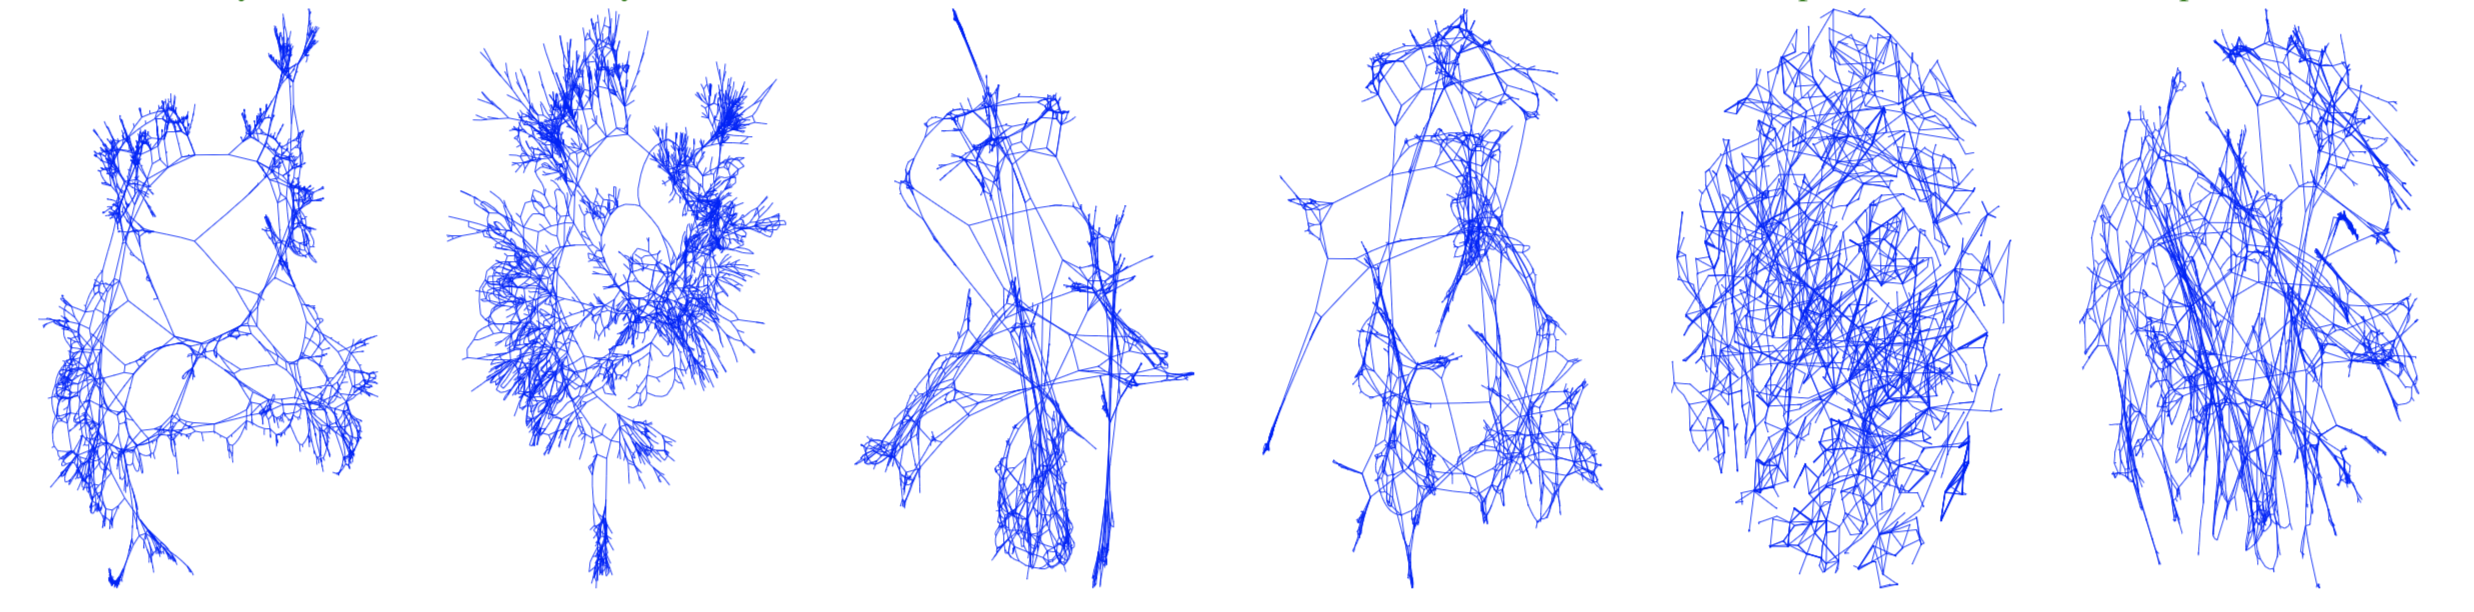
\includegraphics[height=2.05cm,width=0.8\linewidth]{layouts/powernetwork.png}}                                                                                                                \\ \hline
\textbf{add32}   & \multicolumn{6}{c|}{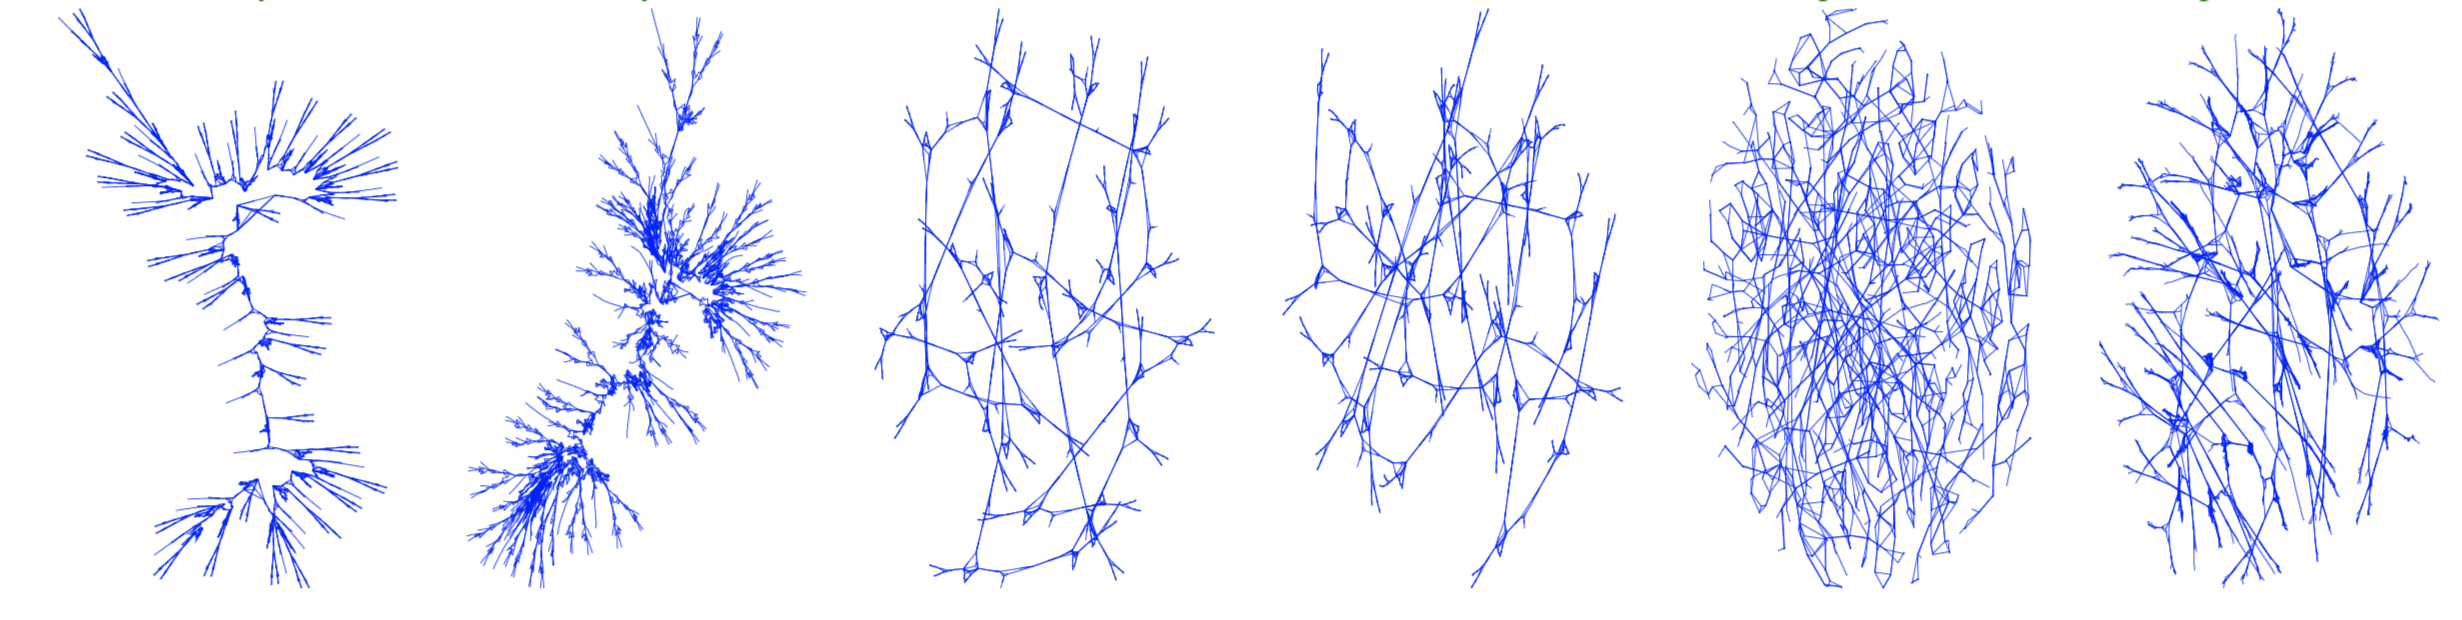
\includegraphics[height=2.05cm,width=0.8\linewidth]{layouts/add32.png}}                                                                                                                 \\ \hline
\textbf{ba\_network}        & \multicolumn{6}{c|}{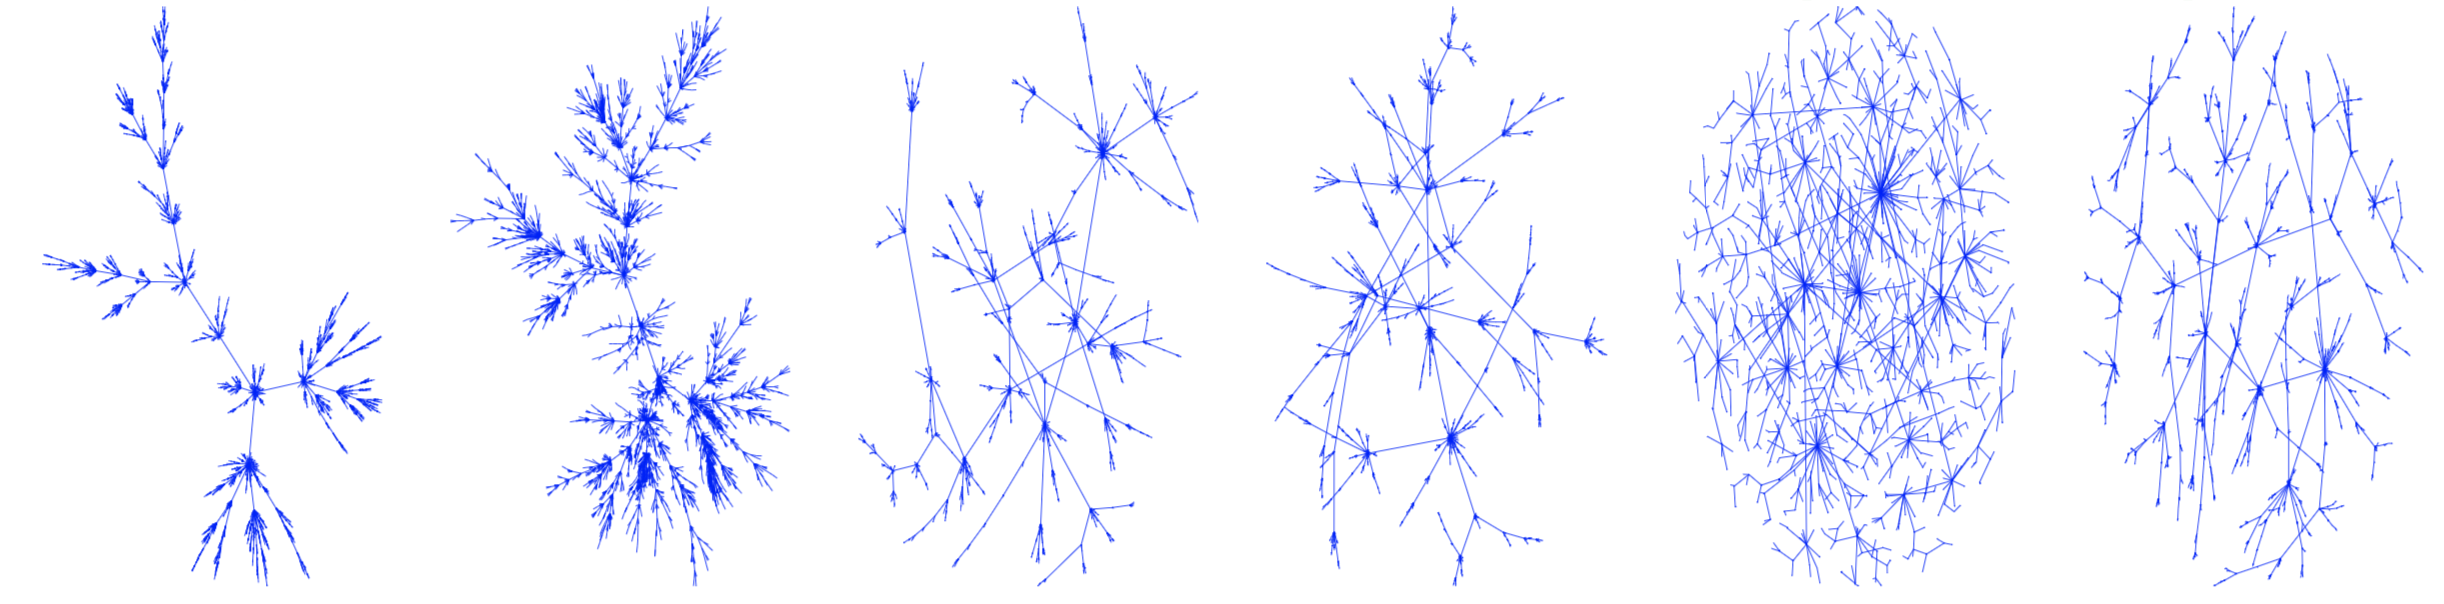
\includegraphics[height=2.05cm,width=0.8\linewidth]{layouts/sf_6000.png}}                                                                                                                 \\ \hline
\textbf{3elt\_dual}        & \multicolumn{6}{c|}{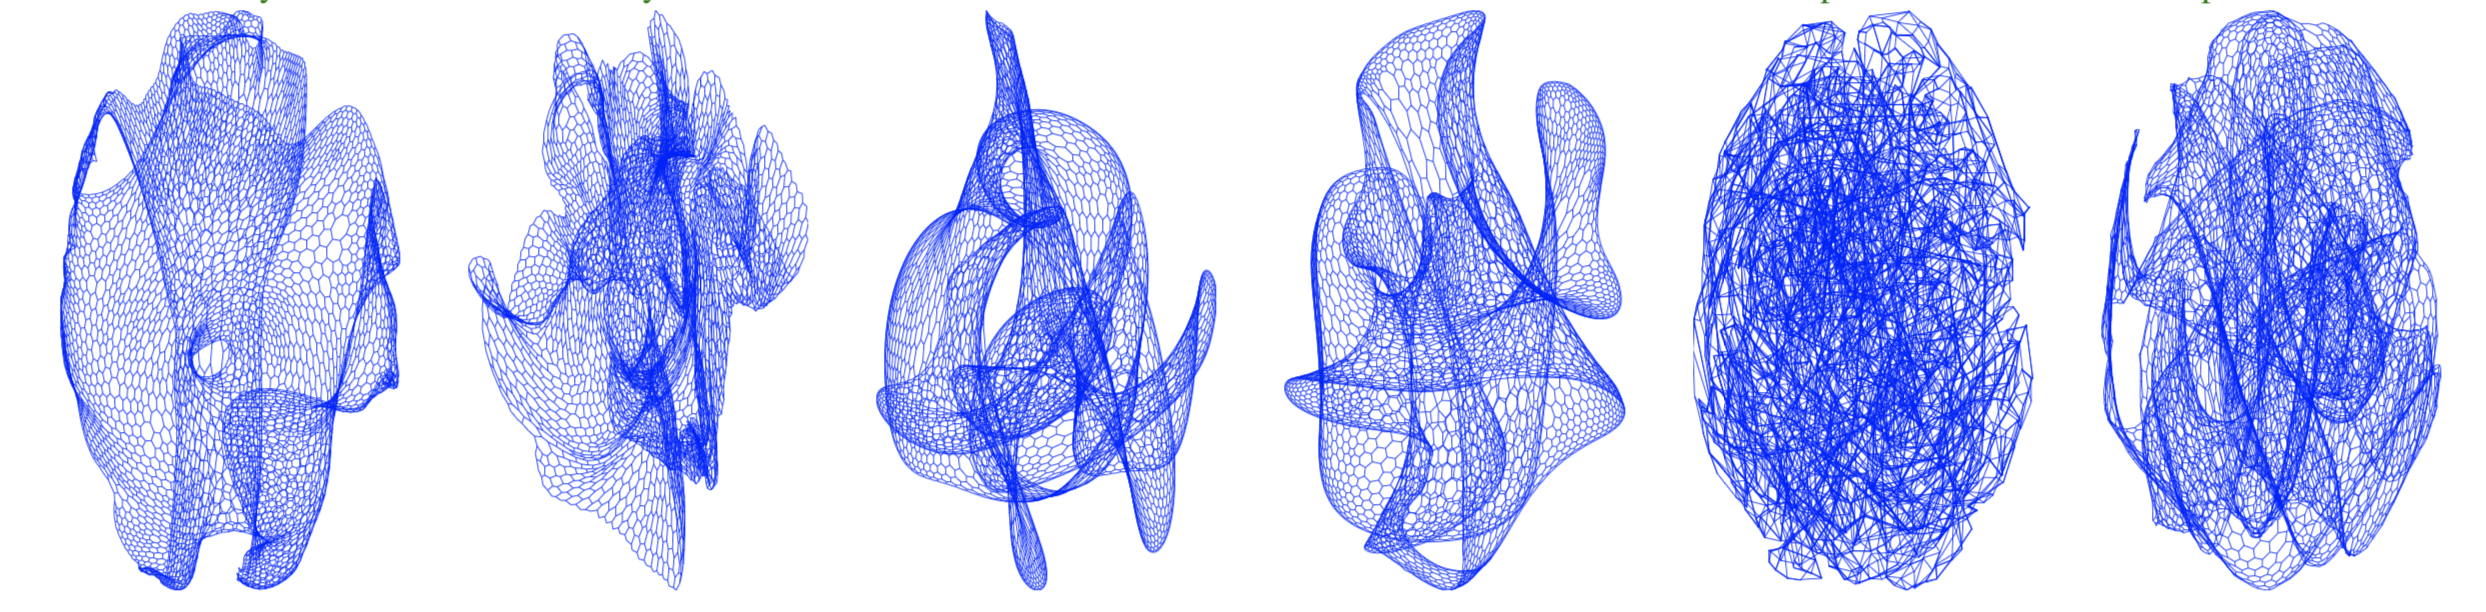
\includegraphics[height=2.05cm,width=0.8\linewidth]{layouts/3elt_dual.png}}                                                                                                                 \\ \hline
\textbf{PGPgiant.}        & \multicolumn{6}{c|}{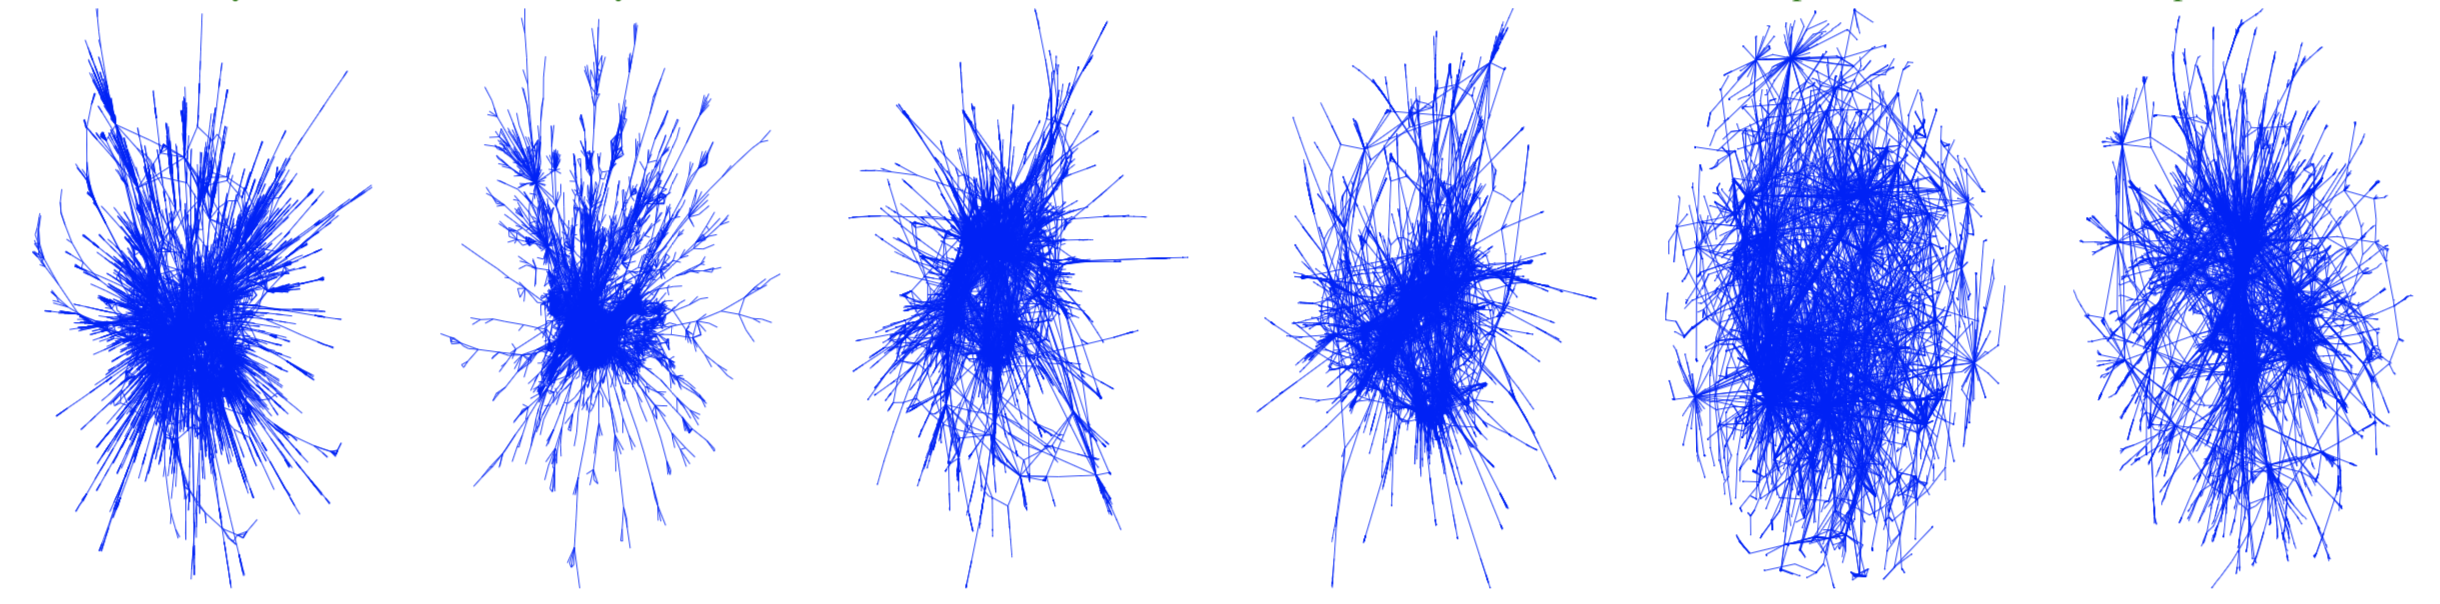
\includegraphics[height=2.05cm,width=0.8\linewidth]{layouts/PGPgiantcompo.png}}                                                                                                                 \\ \hline
\textbf{pkustk02}        & \multicolumn{6}{c|}{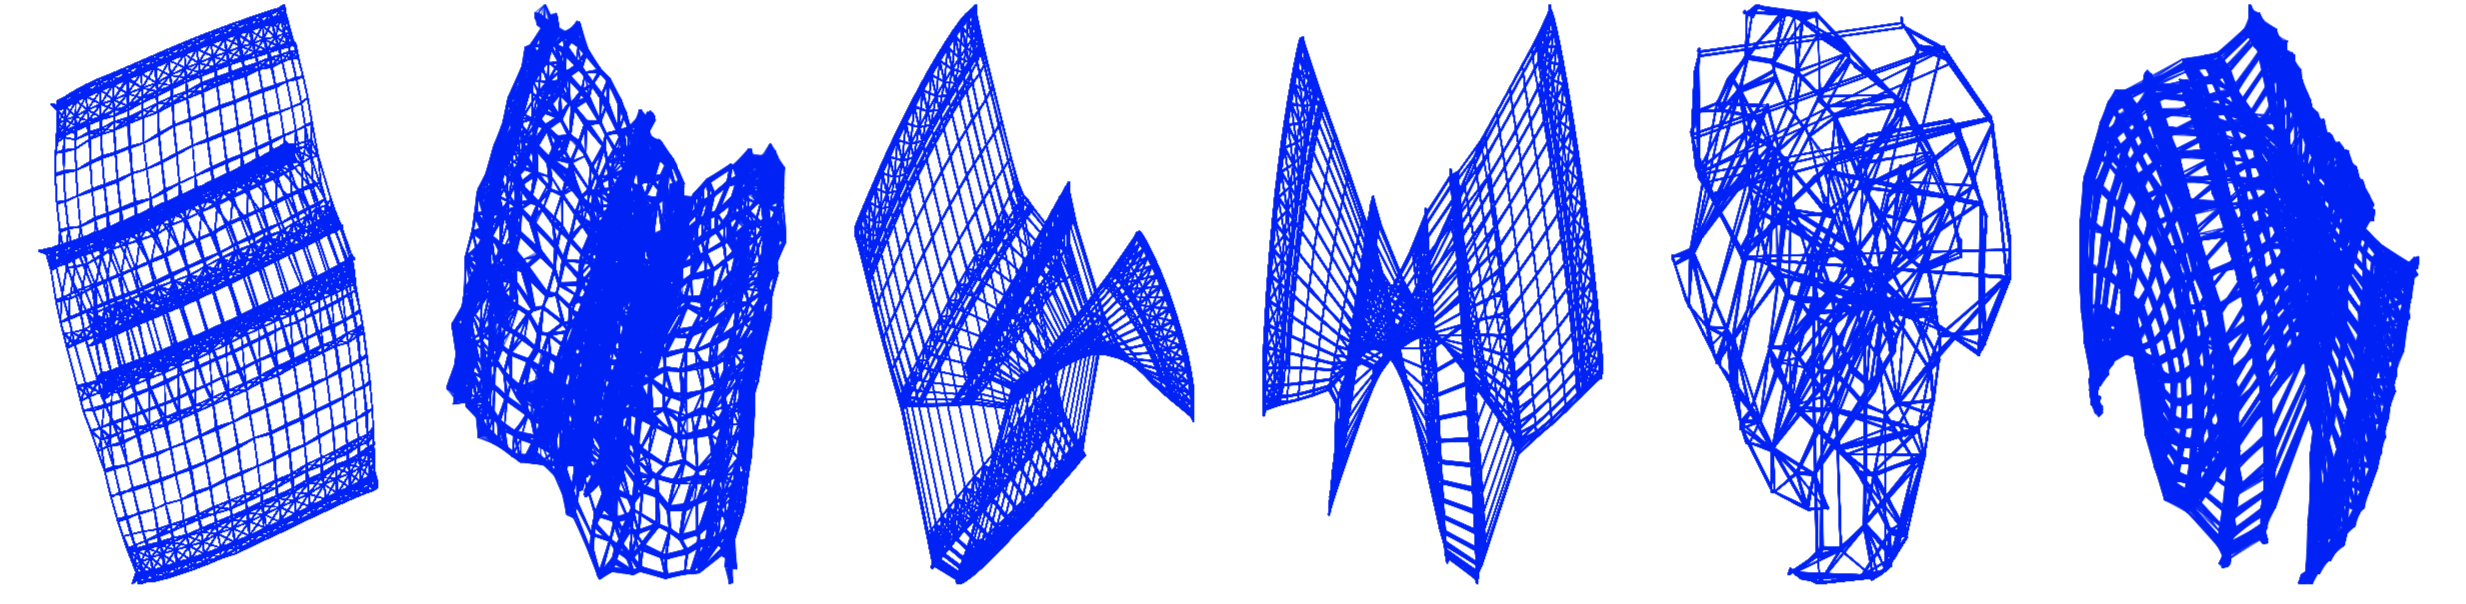
\includegraphics[height=2.05cm,width=0.8\linewidth]{layouts/pkustk02.png}}                                                                                                                 \\ \hline
\textbf{fe\_4elt2}        & \multicolumn{6}{c|}{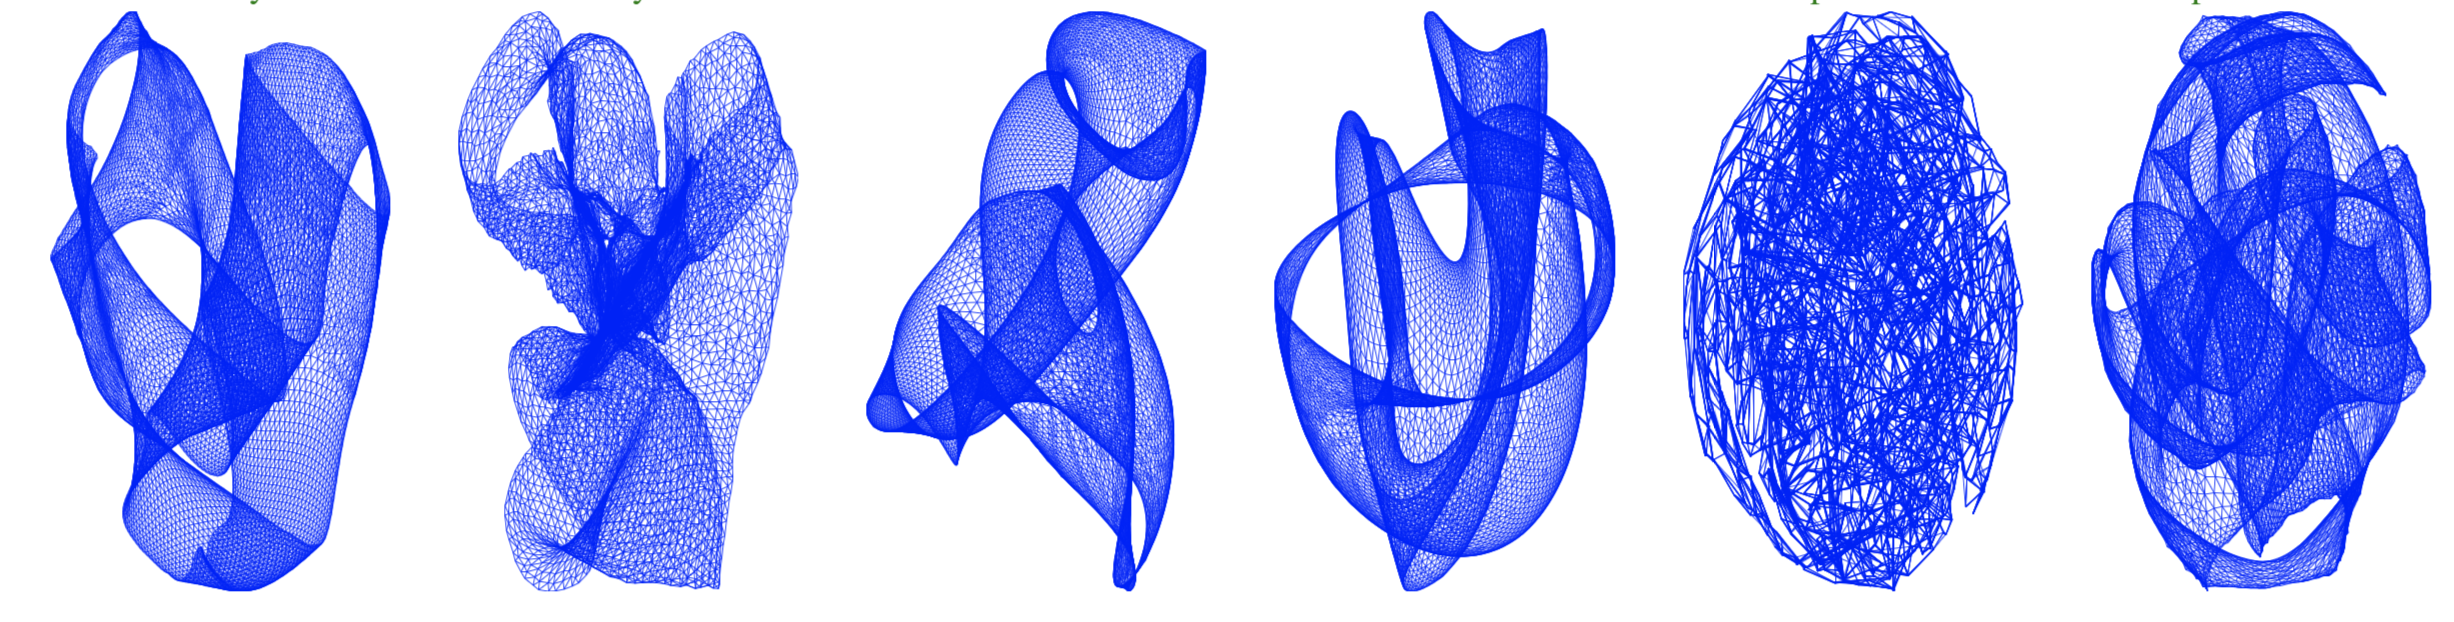
\includegraphics[height=2.05cm,width=0.8\linewidth]{layouts/fe_4elt2.png}}                                                                                                                 \\ \hline
\textbf{bodyy6}        & \multicolumn{6}{c|}{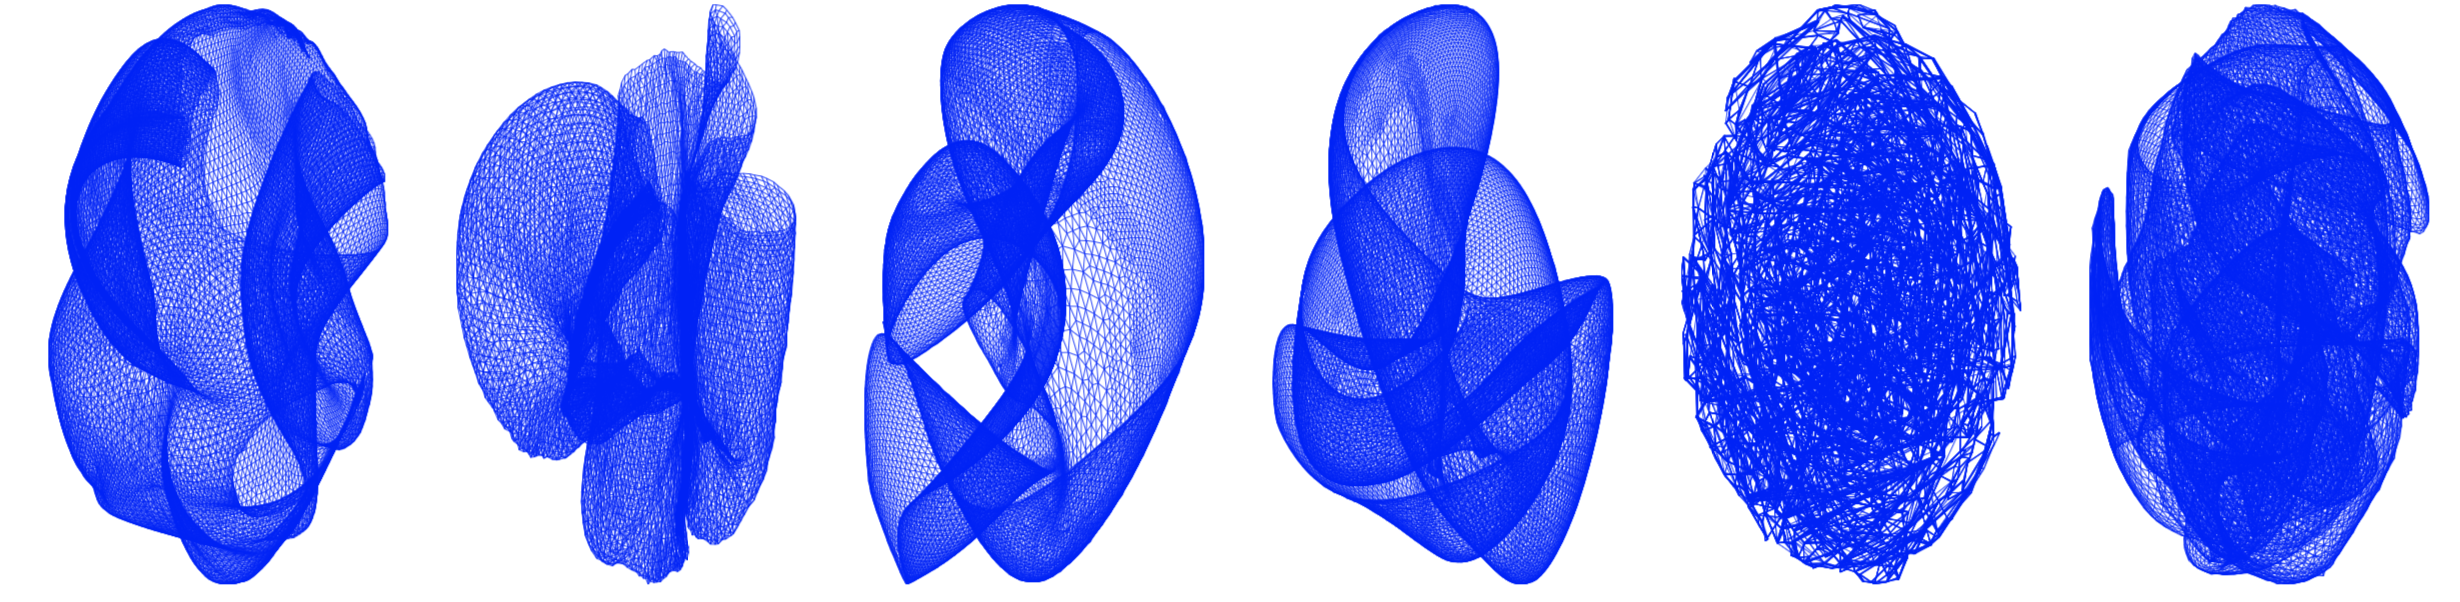
\includegraphics[height=2.05cm,width=0.8\linewidth]{layouts/bodyy6.png}}                                                                                                                 \\ \hline

\textbf{pkustk01}        & \multicolumn{6}{c|}{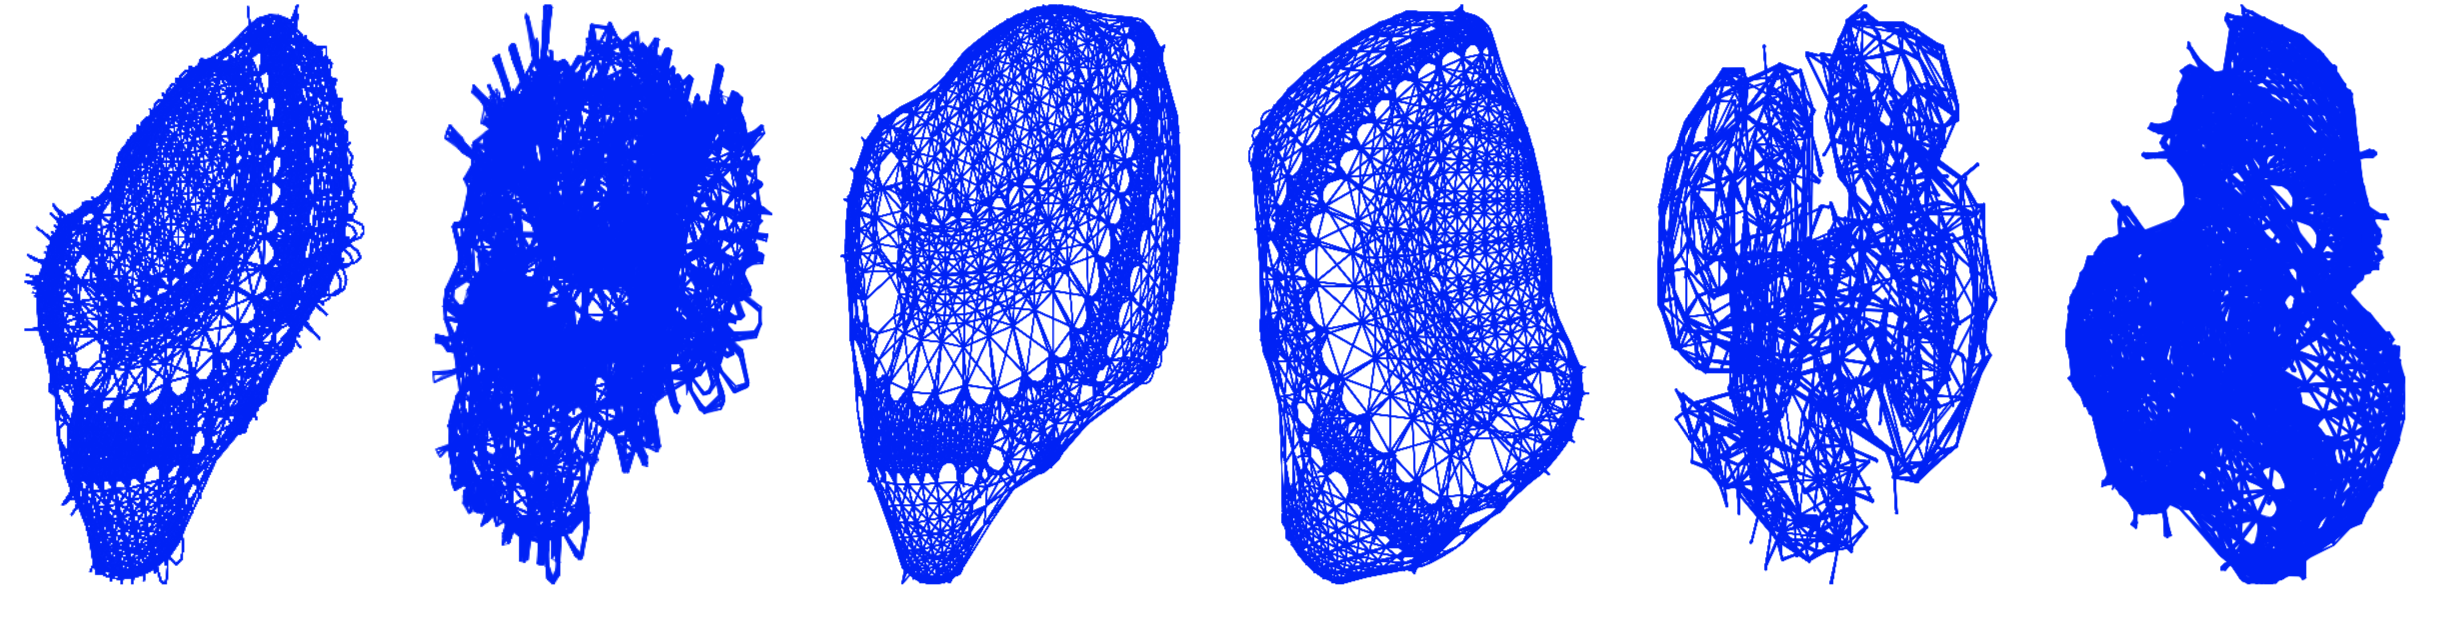
\includegraphics[height=2.05cm,width=0.8\linewidth]{layouts/pkustk01.png}}  \\ \hline

\end{tabular}
\end{table*}

% Please add the following required packages to your document preamble:
% 
% If you use beamer only pass "xcolor=table" option, i.e. \documentclass[xcolor=table]{beamer}
\begin{table}[!htb]
\caption{Convergence of BatchLayout for a threshold value of 1E-6 and values of `Iteration' and `Energy' are for converged layouts. Running time in seconds for other tools for corresponding number of iterations that BatchLayout takes to converged.}
\centering
\label{tab:contime}
\begin{tabular}{|c|c|c|
>{\columncolor[HTML]{C0C0C0}}c |
>{\columncolor[HTML]{C0C0C0}}c |
>{\columncolor[HTML]{C0C0C0}}c |
>{\columncolor[HTML]{C0C0C0}}c |
>{\columncolor[HTML]{C0C0C0}}c |}
\hline
\textbf{Graph} & \textbf{Iter.} & \textbf{Energy} & \textbf{BL} & \textbf{FA2} & \textbf{OO} & \textbf{BLBH}  & \textbf{FA2BH} \\ \hline
power\_grid    & 12445                 & 0.036              & \textbf{26.95}   & 553.25            & 31.83                 & 26.99          & 65.32          \\ \hline
ba\_network    & 9216                  & 13.92              & 28.71            & 461.92            & 29                    & \textbf{23.7}  & 59.69          \\ \hline
3elt\_dual     & 1410                  & 1.3E6           & 8.58             & 160.29            & 6.99                  & \textbf{4.21}  & 13.18          \\ \hline
pkustk02       & 1792                  & 2.9E7           & 15.95            & 377.17            & 12.75                 & \textbf{7.52}  & 40.8           \\ \hline
fe\_4elt2      & 3590                  & 298895             & 32.33            & 591.76            & 21.66                 & \textbf{11.99} & 42.92          \\ \hline
bodyy6         & 2042                  & 7.5E6           & 52.2             & 708.63            & 21.51                 & \textbf{11.15} & 39.58          \\ \hline
pkustk01       & 8995                  & 35.853             & 305.49           & 5231.91           & 119.67                & \textbf{72}    & 305.11         \\ \hline
finance256     & 3747                  & 8.5E6           & 354.43           & 4846.48           & 75.19                 & \textbf{40.19} & 152.44         \\ \hline
\end{tabular}
\end{table}


\begin{table}[!htp]
\caption{Distribution of loops for OpenOrd tool used in Table \ref{tab:contime}}
\centering
\begin{tabular}{|c|c|c|c|c|c|c|}
\hline
\textbf{OpenOrd} & \textbf{25\%} & \textbf{25\%} & \textbf{25\%} & \textbf{10\%} & \textbf{15\%} & \textbf{total 100\%} \\ \hline
power\_grid      & 3111          & 3111          & 3111          & 1245          & 1867          & 12445                \\ \hline
ba\_network      & 2304          & 2304          & 2304          & 922           & 1382          & 9216                 \\ \hline
3elt\_dual       & 353           & 353           & 353           & 141           & 210           & 1410                 \\ \hline
pkustk02         & 448           & 448           & 448           & 179           & 269           & 1792                 \\ \hline
fe\_4elt2        & 898           & 898           & 898           & 359           & 537           & 3590                 \\ \hline
bodyy6           & 511           & 511           & 511           & 204           & 305           & 2042                 \\ \hline
pkustk01         & 2249          & 2249          & 2249          & 900           & 1348          & 8995                 \\ \hline
finance256       & 937           & 937           & 937           & 375           & 561           & 3747                 \\ \hline

\end{tabular}
\end{table}


\begin{table}[!htp]
\centering
\caption{Layouts of \emph{3elt\_dual.mtx} graph generated by BatchLayout for different iterations and batches. BS - batch size. Number in each column represents number of iteration and each row represents size of a batch.}
\label{tab:gridlayout}

\begin{tabular}{|p{1.7cm}|p{1.3cm}|p{1.3cm}|p{1.3cm}|p{1.3cm}|p{1.3cm}|p{1.3cm}|}
\hline
\textbf{}   & \textbf{300} & \textbf{600} & \textbf{900} & \textbf{1200} & \textbf{1500} & \textbf{1800} \\ \hline
        \textbf{BS=1} & \multicolumn{6}{|c|}{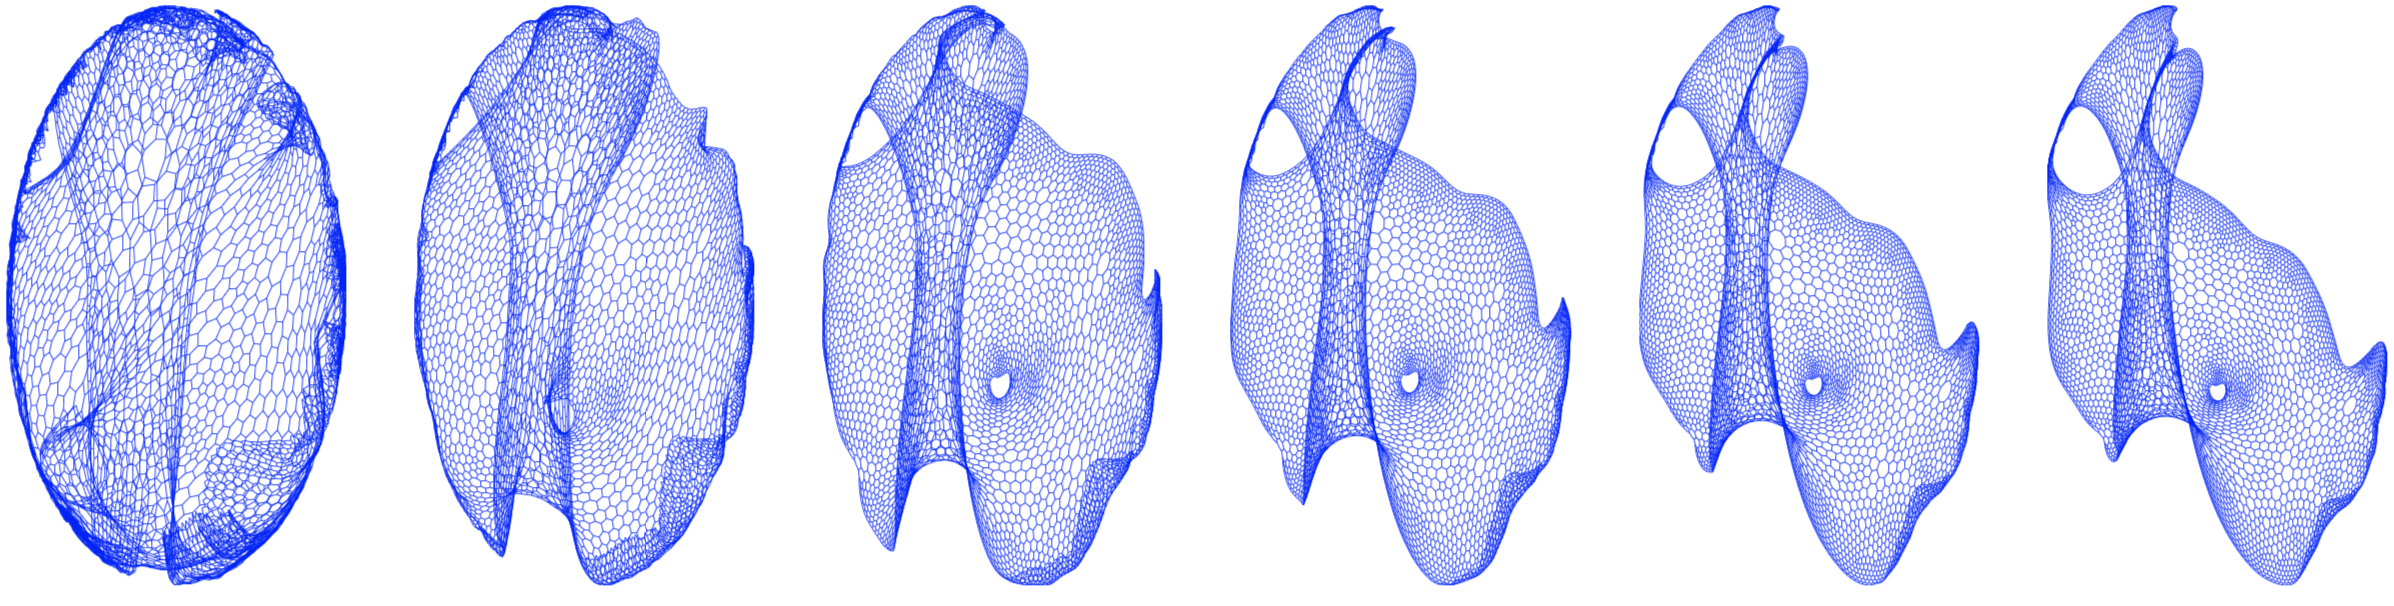
\includegraphics[height=2.2cm,width=0.8\linewidth]{layouts/batches/batch1.png}}                                                                                                                \\ \hline

    \textbf{BS=8} & \multicolumn{6}{|c|}{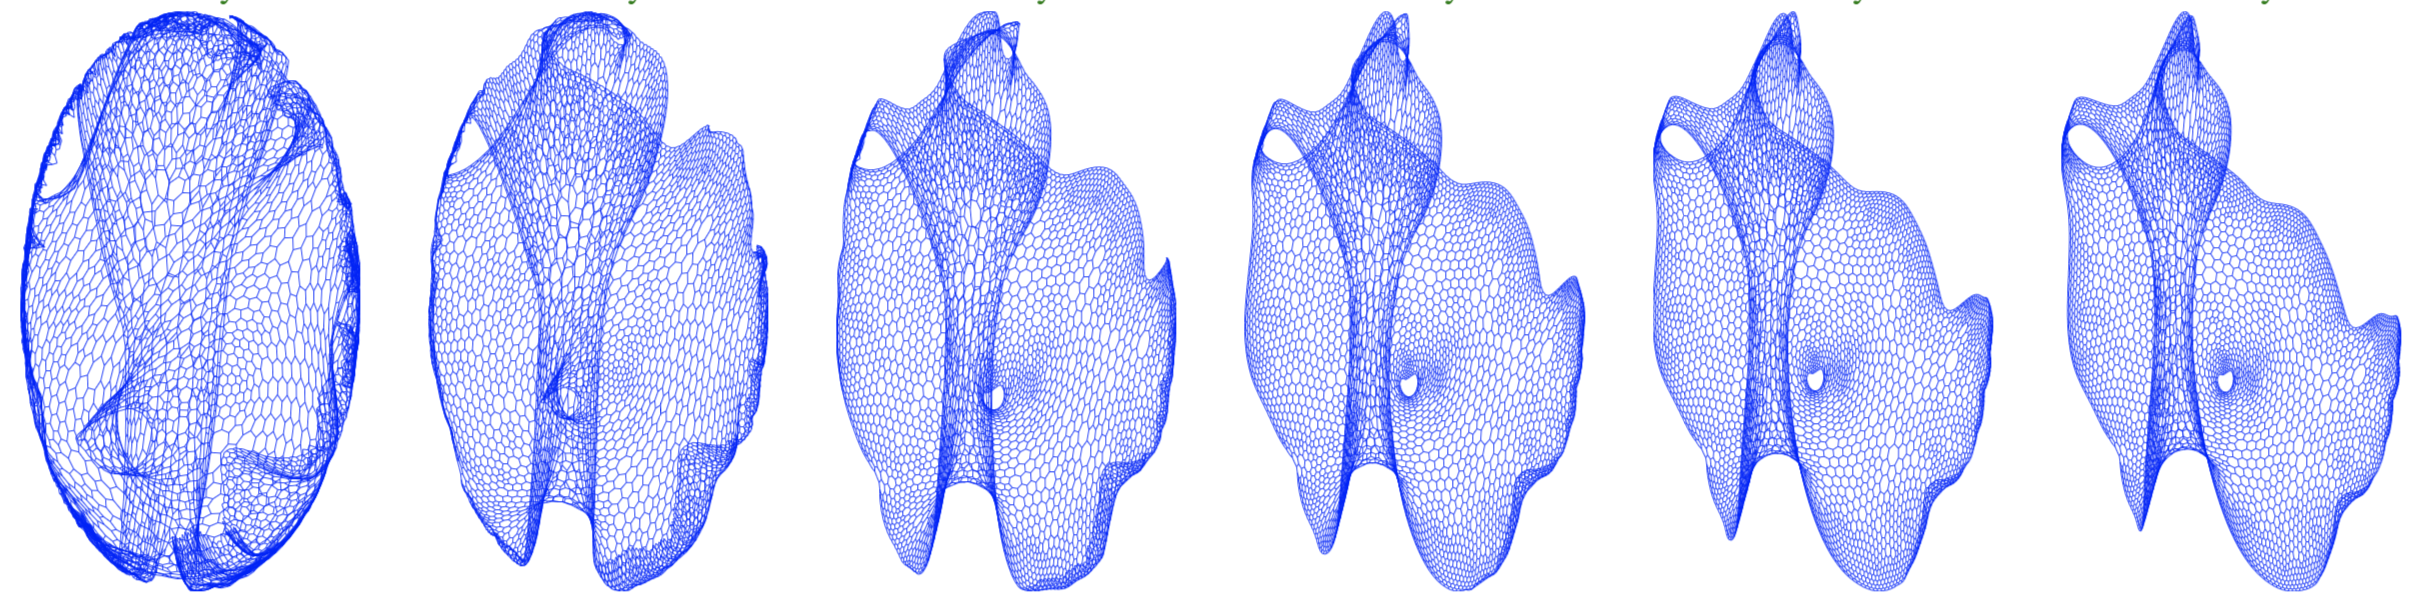
\includegraphics[height=2.2cm,width=0.8\linewidth]{layouts/batches/batch8.png}}                                                                                                                \\ \hline
    
            \textbf{BS=64} & \multicolumn{6}{|c|}{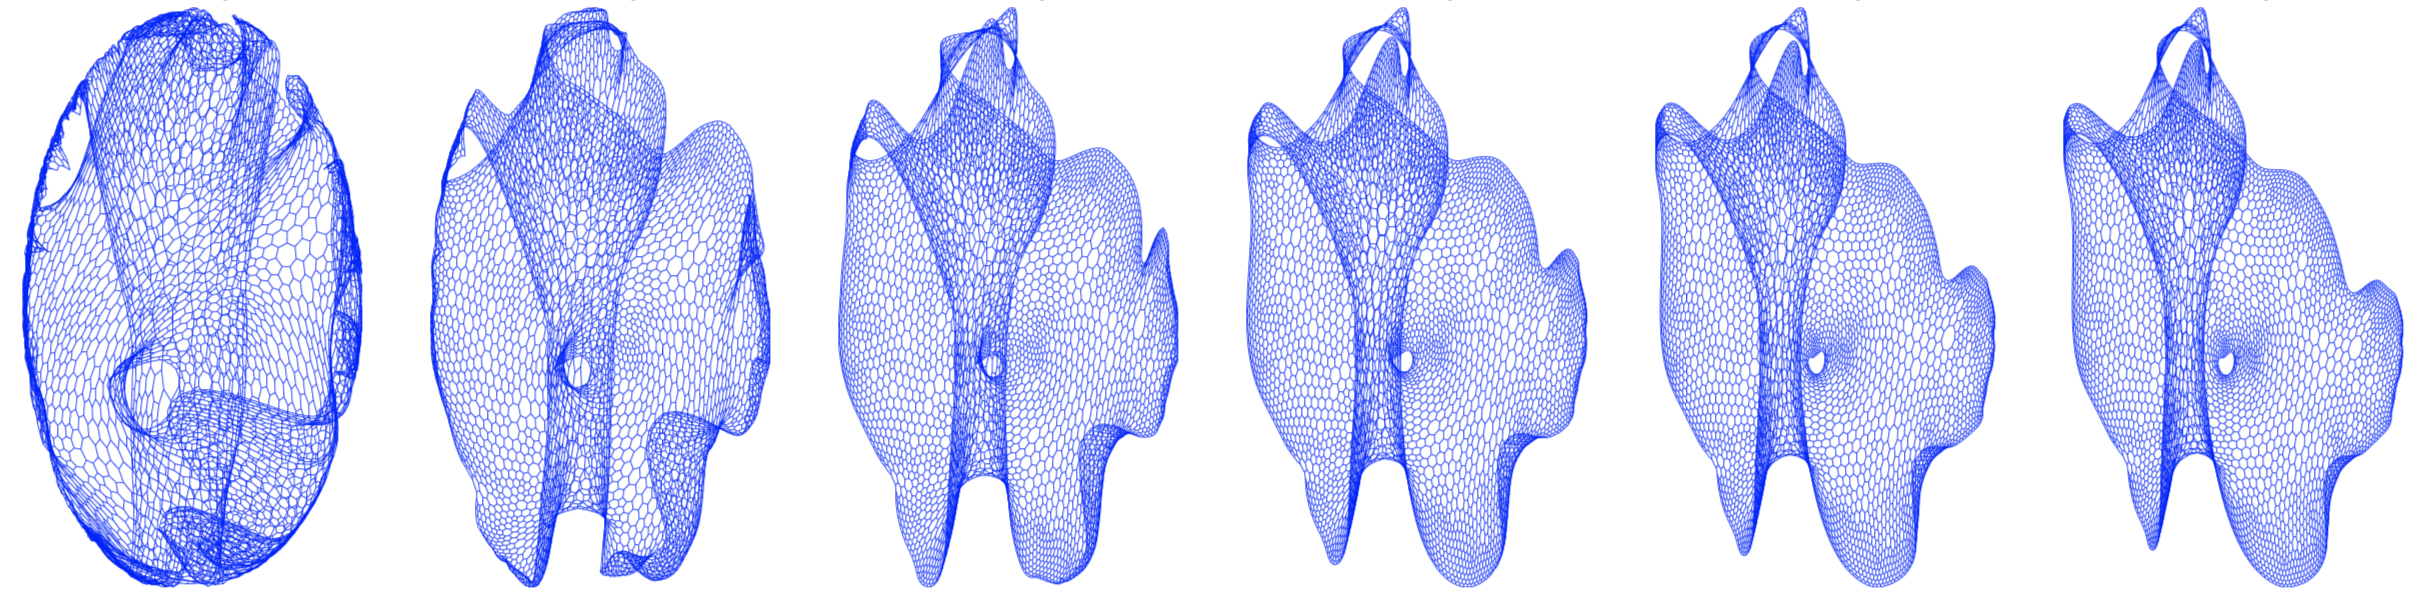
\includegraphics[height=2.2cm,width=0.8\linewidth]{layouts/batches/batch64.png}}                            \\ \hline
            
            \textbf{BS=256} & \multicolumn{6}{|c|}{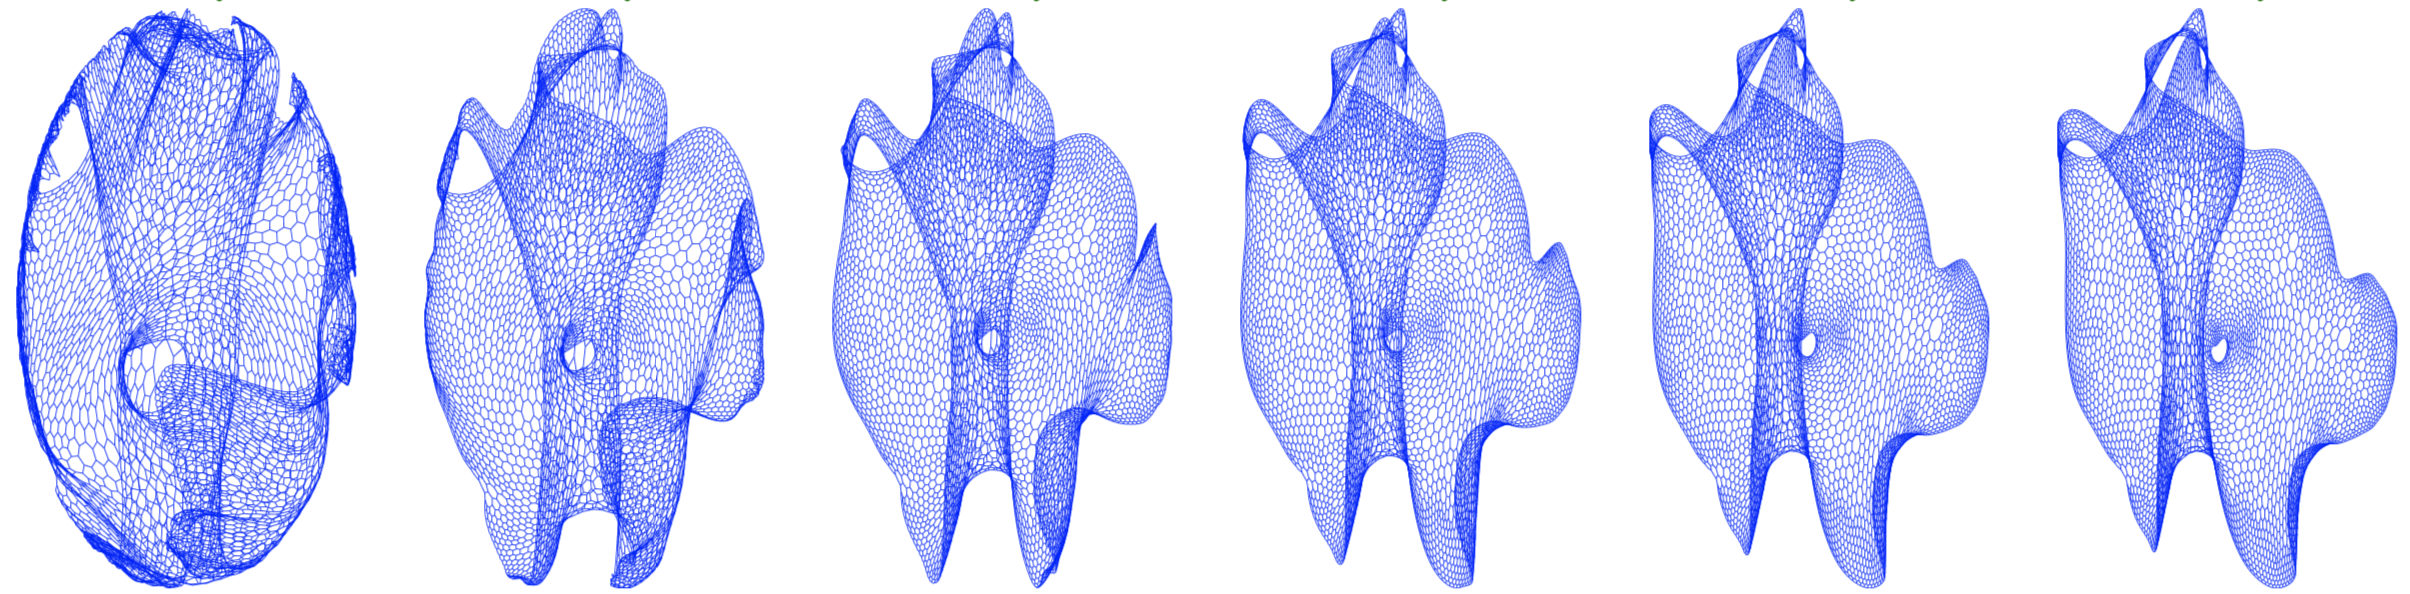
\includegraphics[height=2.2cm,width=0.8\linewidth]{layouts/batches/batch256.png}}                              \\ \hline
    \textbf{BS=1024} & \multicolumn{6}{|c|}{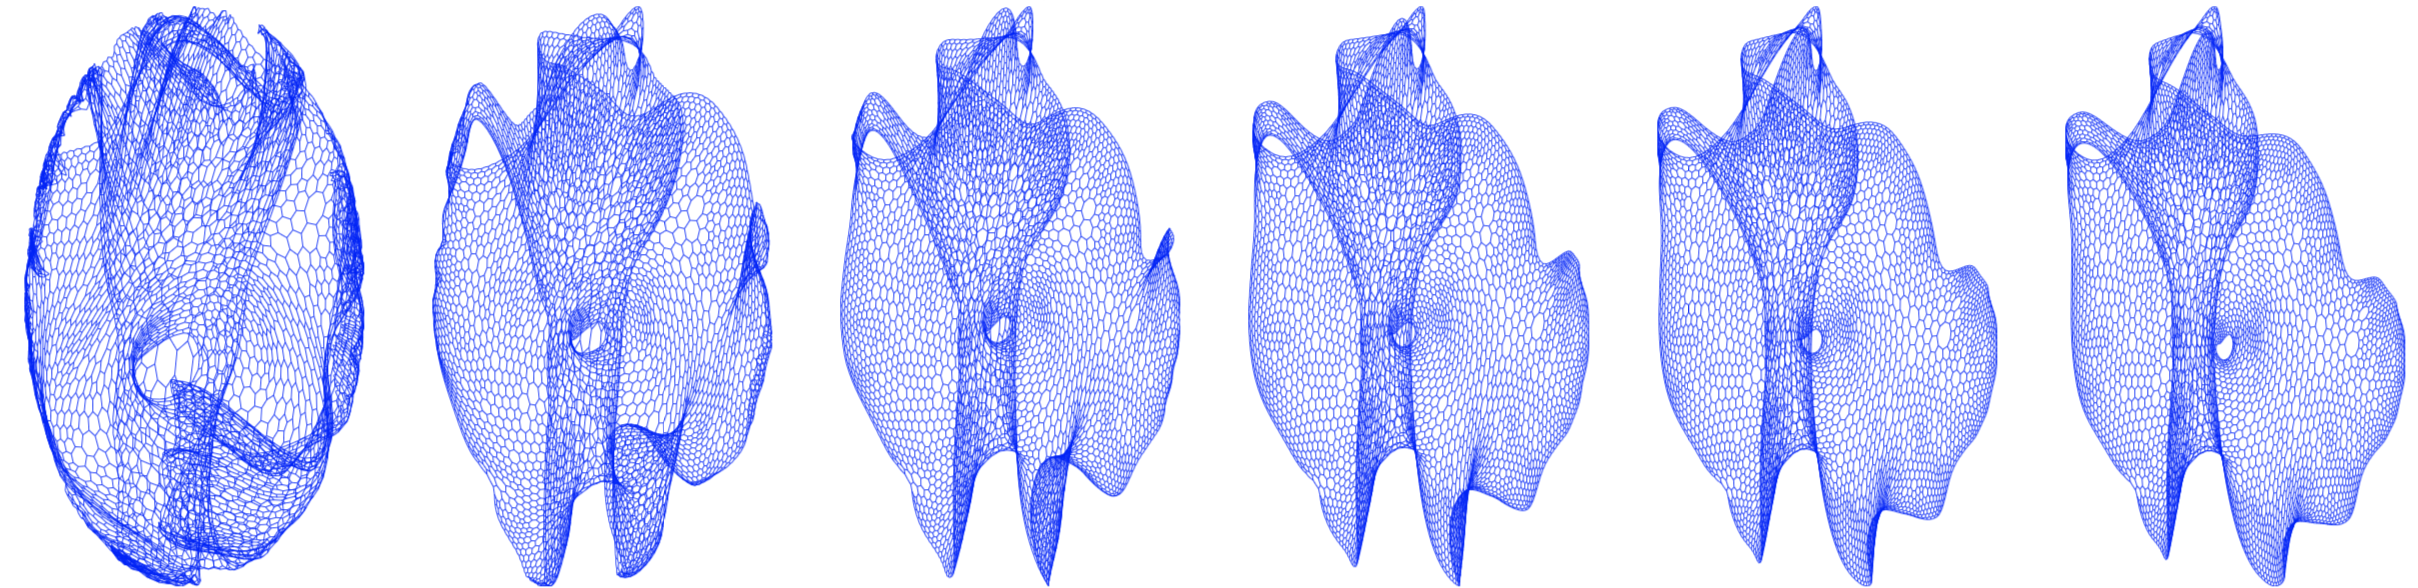
\includegraphics[height=2.2cm,width=0.8\linewidth]{layouts/batches/batch1024.png}}                              \\ \hline
    \textbf{BS=2048} & \multicolumn{6}{|c|}{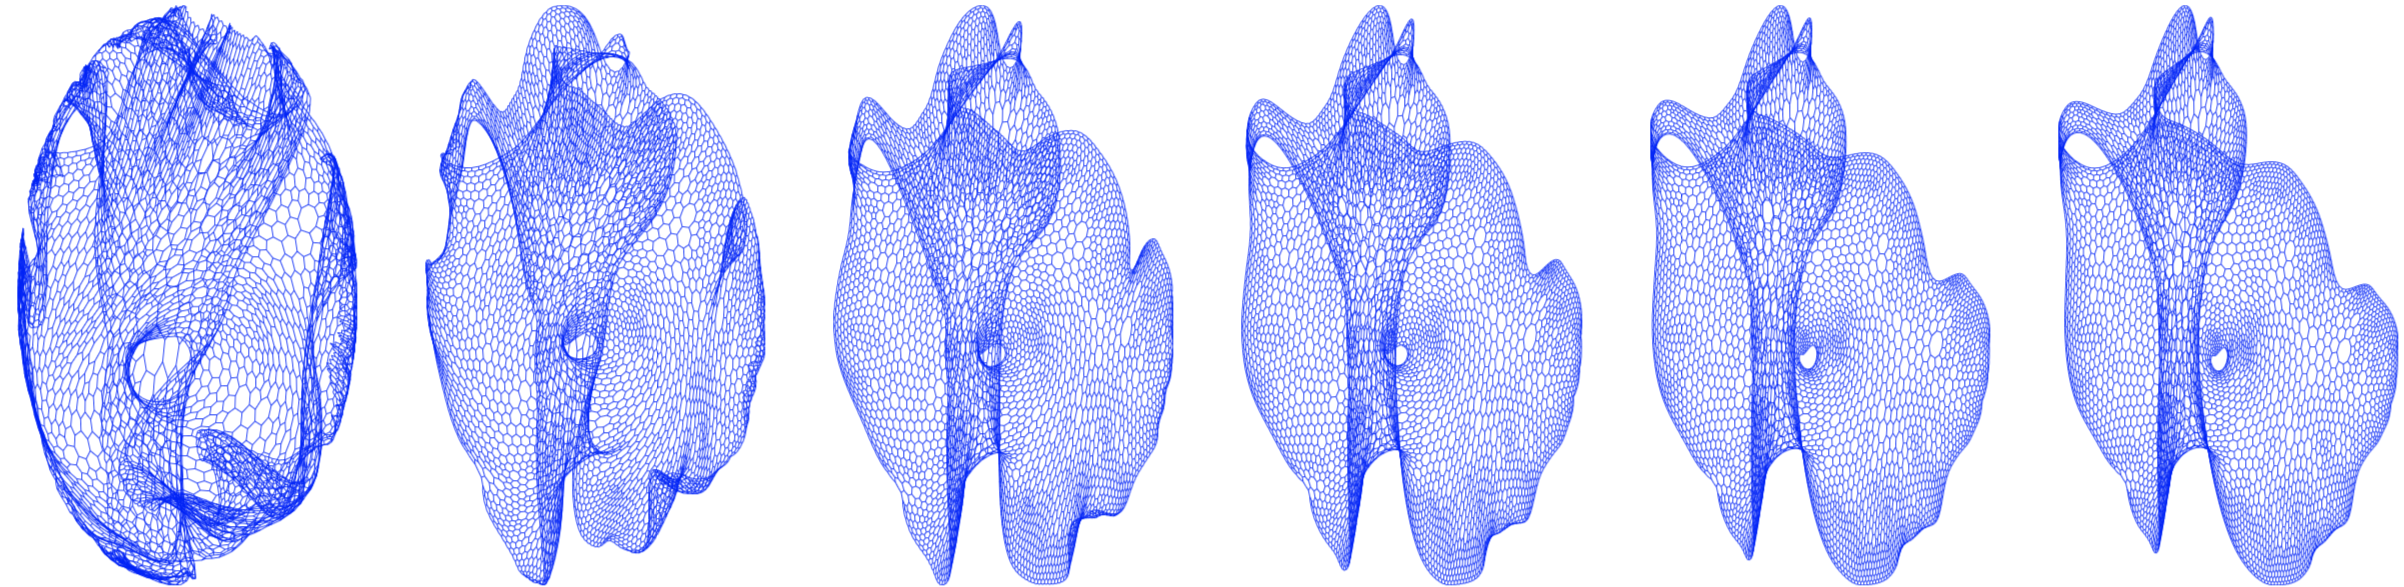
\includegraphics[height=2.2cm,width=0.8\linewidth]{layouts/batches/batch2048.png}}                              \\ \hline
            
\end{tabular}
\end{table}

\section{How to run other tools}

We have used Gephi's toolkit to run ForceAtlas2 and OpenOrd. This integrated tool is available in our repository with proper documentation. Please check out our repository for more details. We have also used OpenOrd tool from authors repository which is written in C++ language using MPI.

\noindent{}\noindent{}\noindent{}To run Gephi's ForceAtlas2, we use commands like following:

\begin{markdown}
```
java -jar othertools/GephiLayouts-1.0.jar forceatlas2 -i 3elt_dual.gml -o 3elt_dual.forceatlas2.gml -threads 8 -maxiters 600
```
\end{markdown}
\newline
\noindent{}\noindent{}\noindent{}To run Gephi's OpenOrd, we use commands like following:

\begin{markdown}
```
java -jar othertools/GephiLayouts-1.0.jar openord -i 3elt_dual.gml -o 3elt_dual.forceatlas2.gml -threads 8 -maxiters 600
```
\end{markdown}
\newline
\noindent{}\noindent{}\noindent{}To run MPI version of OpenOrd, we use commands like following:

\begin{markdown}
```
mpirun --oversubscribe -n 48 ./bin/layout ./input/3elt_dual
```
\end{markdown}
\newline
\noindent{}\noindent{}\noindent{}To run tsNET, we use commands like following:

\begin{markdown}
```
python tsnet.py 3elt_dual.vna --output 3elt_dual.out.vna --perplexity 800 --learning_rate 6000
```
\end{markdown}

\begin{table*}[t]
\caption{Running time of BatchLayout of $O(n^2)$ version for different graphs. We set number of iterations to 500 and enable \emph{-ffast-math -mavx512f -mavx512dq} flags which are available in our Skylake server.}

\centering
\begin{tabular}{|c|c|c|c|}
\hline
\textbf{Graph} & \textbf{Runtime(sec.)} & \textbf{Graph} & \textbf{Runtime(sec.)} \\ \hline

Powergrid &	0.86	 &	add32 &	0.88	\\ \hline
ba\_network  &	1.27 &	3elt\_dual & 2.38 \\ \hline	PGPgiantcompo &	3.27 & pkustk02 &	3.34 \\ \hline
fe\_4elt2 &	3.43	&		bodyy6 &	9.49 \\ \hline	pkustk01 &		12.27 &	OPF\_6000 &		22.37 \\ \hline finance256  & 34.5 &		finan512 & 131.73\\ \hline
\end{tabular}
\label{tab:measures_batchlayout_time}
\end{table*}

\begin{table*}%[t]
\caption{Running time of tsNET for different graphs. tsNET failed to run for finance256 and other graphs which have more vertices than finance256.}

\centering
\begin{tabular}{|c|c|c|c|}
\hline
\textbf{Graph} & \textbf{Runtime(sec.)} & \textbf{Graph} & \textbf{Runtime(sec.)} \\ \hline

Powergrid &	1465.63	 &	add32 &	712.68	\\ \hline
ba\_network  &	2208.14 &	3elt\_dual & 3336.54 \\ \hline	PGPgiantcompo &	7546.79 & pkustk02 &	4195.17 \\ \hline
fe\_4elt2 &	5707.4	&		bodyy6 &	26923.84 \\ \hline	pkustk01 &		26953 &	OPF\_6000 &		60557.65 \\ \hline finance256  & - &		finan512 & -\\ \hline
\end{tabular}
\label{tab:measures_tsnet_time}
\end{table*}



\begin{table*}%[t]
\caption{Comparision of Edge uniformity (EU) measures among random initialized version of \toolname{}. For this measure, lower value means better result.}

\centering
\begin{tabular}{|c|c|c|c|c|c|}
\hline
\multirow{1}{*}{\textbf{Graph}} & \multicolumn{2}{c|}{\textbf{EU}}  &  \multirow{1}{*}{\textbf{Graph}}
& \multicolumn{2}{c|}{\textbf{EU}}            \\ \cline{2-3} \cline{5-6}
                                & BLR       & BLRBH & & BLR & BLRBH  \\ \hline

Powergrid &		0.784 &		0.529 & plustk02	& 	0.844 &		0.699\\ \hline
add32 &	1.354 &		1.029 &	 fe\_4elt2 &		0.404 &		0.51\\ \hline
ba\_network	 &	1.016 &		0.566 & bodyy6 &	0.741 &		0.806 \\ \hline
3elt\_dual &		0.361 &		0.443 &	pkustk01 &	0.76 &		0.659\\ \hline
PGPgiantcompo &	0.812 &		0.704 & - &		- &	-\\ \hline

\end{tabular}
\label{tab:measures_random_init0}
\end{table*}

\begin{table*}%[t]
\caption{Comparision of Stress (ST) and Neighborhood preservation (NP) measures among random initialized version of \toolname{}. For ST, lower value means better result and for NP, higher value represents better result. }
\centering
\begin{tabular}{|c|c|c|c|c|}
\hline
\multirow{1}{*}{\textbf{Graph}} & \multicolumn{2}{c|}{\textbf{ST}}                            & \multicolumn{2}{c|}{\textbf{NP}}            \\ \cline{2-5} 
                                & BLR       & BLRBH & BLR & BLRBH  \\ \hline

Powergrid	&	1.7E+6	&	2.2E+6	&	0.336 &		0.208\\ \hline
add32	&	2.0E+6	&	2.7E+6	&	0.437	&	0.229\\ \hline
ba\_network	&	2.9E+6	&	2.8E+6	&	0.346	&	0.283\\ \hline
3elt\_dual	&	1.0E+7 &	1.3E+7	&	0.168	&	0.112\\ \hline
PGPgiantcompo	&	8.1E+6 &		1.7E+7	&	0.182	&	0.109\\ \hline
plustk02	&	2.7E+7	&	4.7E+7	&	0.412	&	0.211\\ \hline
fe\_4elt2	&	1.6E+7	&	2.1E+7	&	0.268	&	0.165\\ \hline
bodyy6	&	3.9E+7	&	4.2E+7	&	0.171	&	0.177\\ \hline
pkustk01	&	4.6E+6	&	4.2E+6	&	0.626	&	0.599\\ \hline


\end{tabular}
\label{tab:measures_random_init}
\end{table*}

\begin{figure}
    \centering
    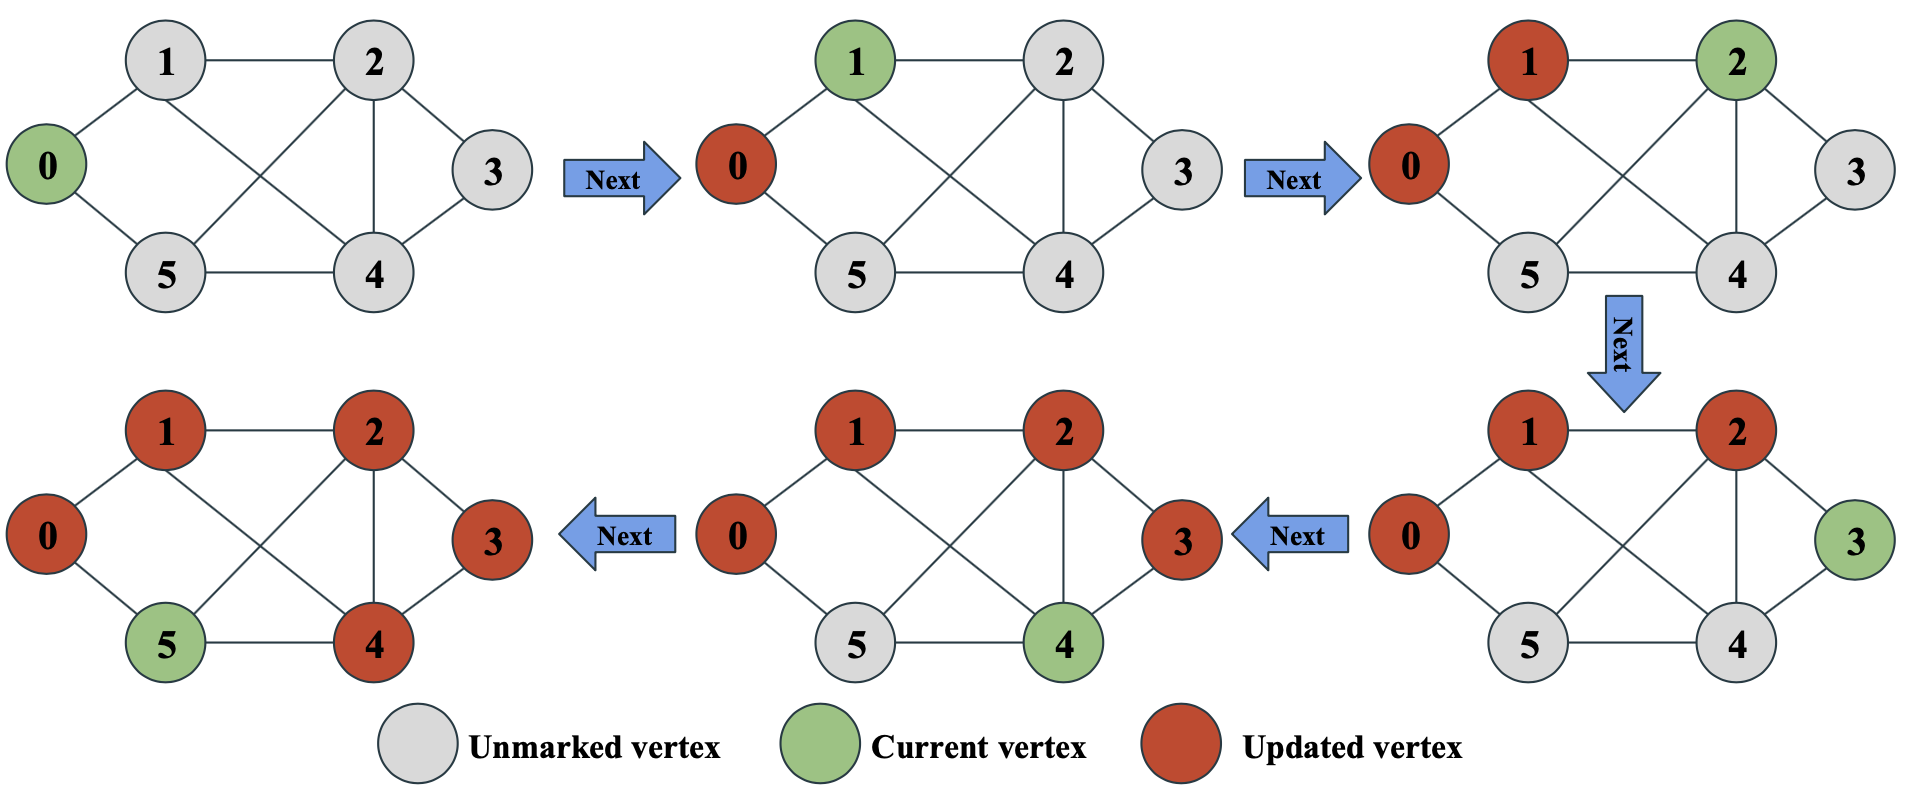
\includegraphics[width=\linewidth]{figures/sgd.png}
    \caption{Example of force calculations in sequential approach. Gray colored vertex represents unmarked vertex whose updated position has neither been calculated nor is being calculated. Green colored vertex represents current vertex whose forces are being calculated with respect to all other vertices. Red colored vertex represents those cases whose forces have already been updated/calculated.}
    \label{fig:sgdfig}
\end{figure}

\begin{figure*}
    \centering
    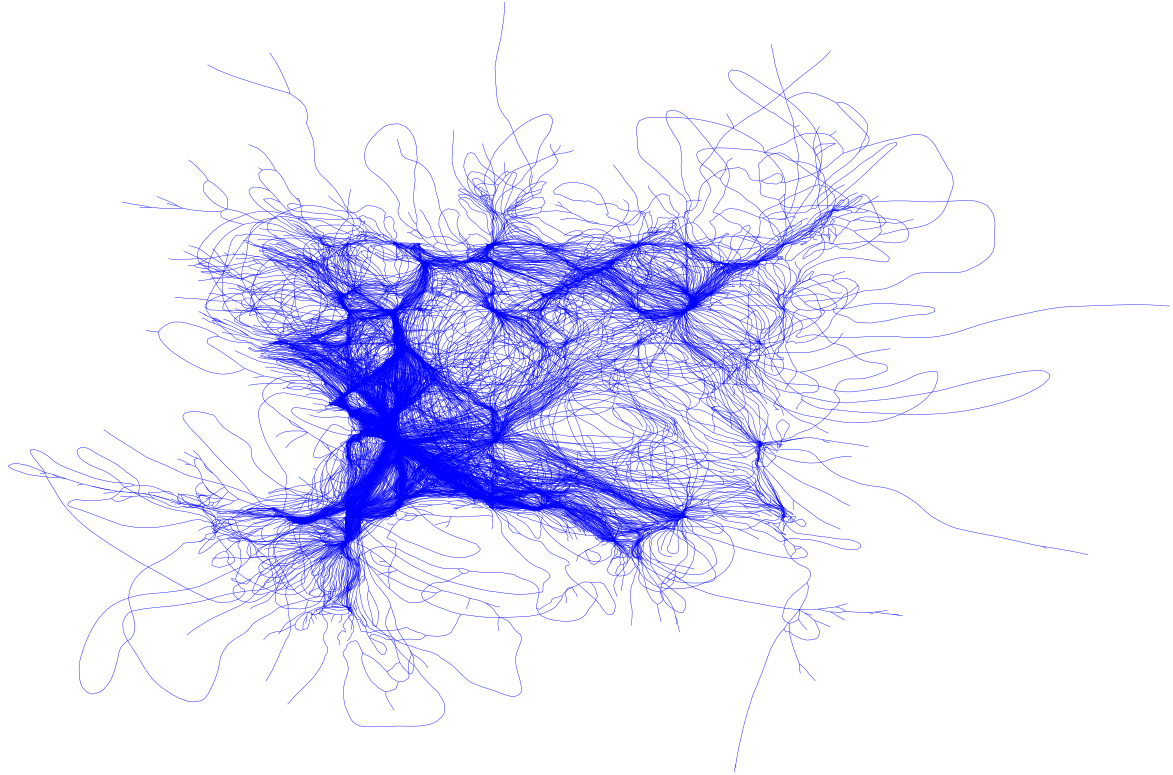
\includegraphics[width=0.32\linewidth]{layouts/BLBHlx750.png}
    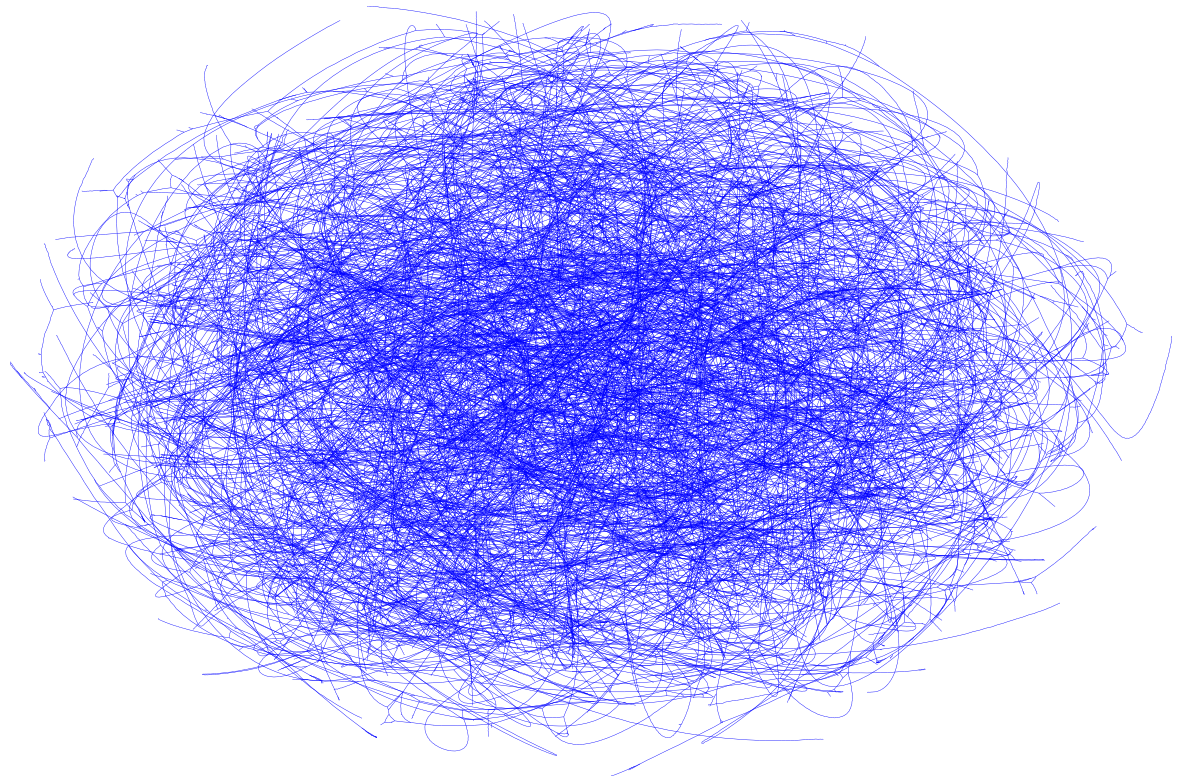
\includegraphics[width=0.32\linewidth]{layouts/FA2BHlx750.png}
    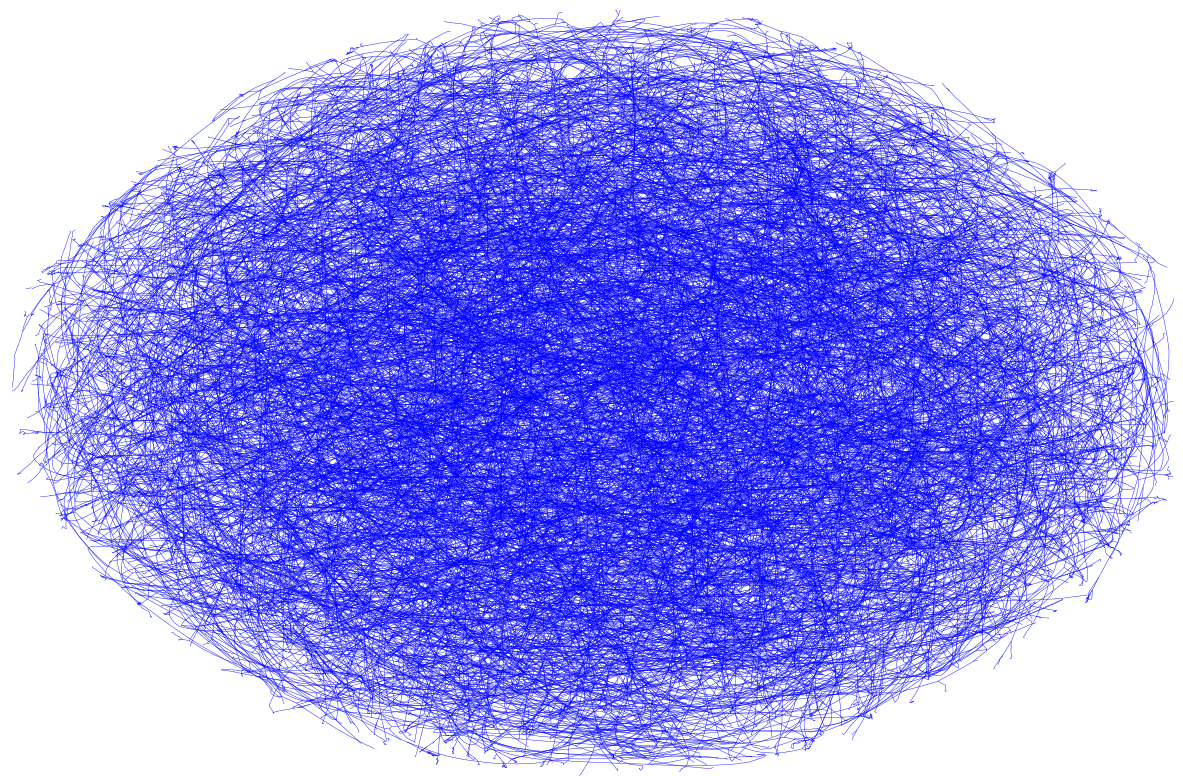
\includegraphics[width=0.32\linewidth]{layouts/OOGHoutput_lxOSM.png}
    \caption{Layouts of lxOSM which has 114,599 vertices and 239,332 edges. BatchLayoutBH (left plot), ForceAtlas2BH (middle plot) and OpenOrd (right plot) took 24.75 seconds, 102.0 seconds and 50.03 seconds, respectively for 750 iterations using 48 threads. \toolnameBH{} is capable of generating readable layout within very short time than other two tools.}
    \label{fig:biggraphs}
\end{figure*}

\begin{figure*}
    \centering
    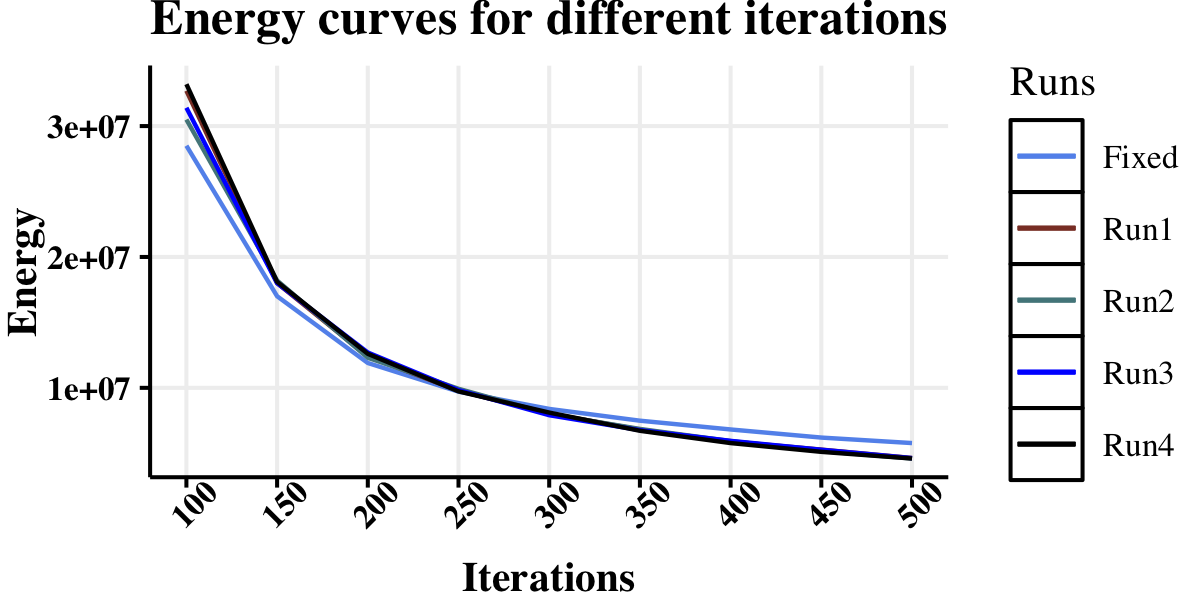
\includegraphics[width=0.48\linewidth]{figures/origrandombatches.png}
     \includegraphics[width=0.48\linewidth]{figures/boxrandombatches.png}
    \caption{Energy curves of random batch selection for different runs with same hyper-parameters (3elt\_dual graph) (left figure). There are differences but due to high value of energy, it is not clearly visible and we demonstrate this difference in right figure.}
    \label{fig:origruns}
\end{figure*}


\begin{figure}
    \centering
    \includegraphics[width=0.7\linewidth]{figures/summary50iterations.pdf}
    \caption{Summary of running time and aesthetic quality of all tools for 500 iterations discussed in the manuscript, Tables II, III and IV. We normalize running time by dividing the maximum running time among all tools for a corresponding graph and subtracting from 1 to feel like higher number is better for quality. We similarly compute other normalized aesthetic measure to set within range 0 to 1 where higher value means better quality. We put normalized running time quality in x-axis and normalized aesthetic measures in y-axis for each corresponding graph. ForceAtlas2 is not shown due to its lower normalized value for running time which is always 0. Obviously, the best tool will touch the right-top corner i.e., better running time as well as better quality. BatchLayout and BatchLayoutBH are shown in same color to distinguish from other tools. We clearly see that BatchLayout and BatchLayoutBH attain better running time and quality.}
    \label{fig:summary500iterations}
\end{figure}

\begin{algorithm}
\caption{constructBHT}
\hspace*{\algorithmicindent} \textbf{Input:} $c$, $D$
\begin{algorithmic}[1]
\State $p_1 \leftarrow$ consecutive $c_i$'s in left top cell
\State $p_2 \leftarrow$ consecutive $c_i$'s in right top cell
\State $p_3 \leftarrow$ consecutive $c_i$'s in left bottom cell
\State $p_4 \leftarrow$ consecutive $c_i$'s in right bottom cell
\State compute diameter $D = \frac{D}{2}$
\State $t_1 \leftarrow$ constructBHT($p_1$, $D$) in parallel
\State $t_2 \leftarrow$ constructBHT($p_2$, $D$) in parallel
\State $t_3 \leftarrow$ constructBHT($p_3$, $D$) in parallel
\State $t_4 \leftarrow$ constructBHT($p_4$, $D$) in parallel
\State check coordinates if any of $t_i$'s is leaf node
\State compute centroid $s$ using $t_1$,$t_2$,$t_3$,and $t_4$
\newline
\Return create tree \emph{node} using $t_1$,$t_2$,$t_3$,$t_4$, $s$, and $D$
\end{algorithmic}
\label{algo:constructbht}
\end{algorithm}


\begin{algorithm}
\caption{calcRepulsiveForce}
\hspace*{\algorithmicindent} \textbf{Input:} $r$, $i$, $f$
\begin{algorithmic}[1]
\State $d = \parallel r_c - i\parallel$ \Comment{Euclidean distance}
\If{$\theta > \frac{D}{d}$} \Comment{MAC condition}
\State $f += f_a(r_c,i)\times \frac{r_c-i}{d}$ \Comment{$r_c$ indicates coordinates of $r$}
\Else 
\For{$child$ of $r$}
\If{$child$ has descendent}
\State calcRepulsiveForce($child$, $i$, $f$)
\Else
\State $f += f_r(child_c,i)\times \frac{child_c-i}{d}$ \Comment{$child_c$ indicates coordinates of $child$}
\EndIf
\EndFor
\EndIf
\end{algorithmic}
\label{algo:queryserve}
\end{algorithm}


\begin{algorithm}
\caption{BatchLayoutBH}
\hspace*{\algorithmicindent} \textbf{Input:} G(c, V, E)
\begin{algorithmic}[1]
\State $Step = 1.0$ \Comment{initial step length}
\State $Loop = 0$
\While {$ Loop < MaxIteration$}
\State $Energy = 0$
\State re-scale $c$ in bounding box
\State sort $c$ in parallel based on morton order
\State $D = max(max(c_x)-min(c_x),max(c_y)-min(c_y))$
\State $BHT = constructBHT(c, D)$ \Comment{call Algorithm \ref{algo:constructbht}}
\ParFor{$i \in V$}
			\State $ct_{i} = 0$
\EndParFor
\For{$b \leftarrow$ 0 to $\frac{n}{BS}-1$}
    \ParFor{$i \leftarrow b * BS$ to $(b + 1) * BS-1$ \textbf{by} $bx$}
        \State $f = (0,0)$
        \For{$j\in G.colids[i]$}
                    \State $f\;+= f_a(i,j)\times \frac{c_j - c_i}{||c_i - c_j||}$
        \EndFor 
        \State $calcRepulsiveForce(BHT, i, rf = (0,0))$ \Comment{call Algorithm \ref{algo:queryserve}}
        \State $f = f - rf$;
        \State $ct_{i+x} += f$
    \EndParFor
    \ParFor{$i \leftarrow b * BS $ to $(b + 1) * BS - 1$}
        \State $c_i\; += Step \times \frac{ct_i}{||ct_i||}$
        \State $Energy\; += ||ct_i||^2$
    \EndParFor
\EndFor
\EndWhile
\newline
\Return the final layout $c$
\end{algorithmic}
\label{algo:cbBatchLayout}
\end{algorithm}



\begin{figure}
    \centering
    \includegraphics[width=0.3\linewidth]{figures/batchlayoutsystem.png}
    \caption{BatchLayout system overview. In BatchLayout, we demonstrate two initialization techniques, several energy models and repulsive force approximation techniques, flexibility of choosing batch size and number of threads, evaluation based on run time and aesthetic metrics, and visualization.}
    \label{fig:blsystem}
\end{figure}


\begin{table*}[t]
\caption{Running time of $FM^3$ of OGDF library for different graphs. We run default option of $FM^3$ by setting number of iterations to 500.}

\centering
\begin{tabular}{|c|c|c|c|}
\hline
\textbf{Graph} & \textbf{Runtime(sec.)} & \textbf{Graph} & \textbf{Runtime(sec.)} \\ \hline

Powergrid &	2.21	 &	add32 &	1.34	\\ \hline
ba\_network  &	2.45 &	3elt\_dual & 3.77 \\ \hline	PGPgiantcompo &	5.90 & pkustk02 &	5.27 \\ \hline
fe\_4elt2 &	4.13	&		bodyy6 &	7.75 \\ \hline	pkustk01 &		9.82 &	OPF\_6000 &		11.68 \\ \hline finance256  & 13.33 &		finan512 & 27.89\\ \hline
comYout.  & 897.17 &		Flan\_1565 & 1105.33\\ \hline
\end{tabular}
\label{tab:measures_fm3_time}
\end{table*}

\begin{table*}[]
\caption{Number of edge crossing in the layouts after running each tool for 500 iterations.}
\centering
\begin{tabular}{|c|c|c|c|c|c|}
\hline
\textbf{Graph} & \textbf{BL} & \textbf{BLBH} & \textbf{FA2} & \textbf{FA2BH} & \textbf{OO} \\ \hline
Powergrid      & 3892        & 8030          & 3300         & 3308           & 6631        \\ \hline
add32          & 5745        & 22466         & 1325         & 1608           & 17145       \\ \hline
ba\_network    & 526         & 7518          & 273          & 334            & 588         \\ \hline
3elt\_dual     & 6208        & 12678         & 13992        & 8385           & 24990       \\ \hline
PGPgiant.      & 909233      & 2096136       & 626802       & 632239         & 722747      \\ \hline
fe\_4elt2      & 51472       & 252197        & 67624        & 73995          & 133574      \\ \hline
bodyy6         & 208077      & 363718        & 153062       & 181133         & 475689      \\ \hline
\end{tabular}
\end{table*}

\end{document}
